
\chapter{Teaching Tech Together}\label{teaching-tech-together}

Hundreds of grassroots groups have sprung up around the world to teach
programming, web design, robotics, and other skills to \protect\hyperlink{g:free-range-learner}{free-range
learners} outside traditional classrooms. These
groups exist so that people don't have to learn these things on their
own, but ironically, their founders and instructors are often teaching
themselves how to teach.

There's a better way. Just as knowing a few basic facts about germs
and nutrition can help you stay healthy, knowing a few things about
psychology, instructional design, inclusivity, and community
organization can help you be a more effective teacher. This book
presents evidence-based practices you can use right now, explains why
we believe they are true, and points you at other resources that will
help you go further. Its four sections cover:

\begin{itemize}
\tightlist
\item
  how people learn;
\item
  how to design lessons that work;
\item
  how to deliver those lessons; and
\item
  how to grow a community of practice around teaching.
\end{itemize}

\begin{quote}\setlength{\parindent}{0pt}
\textbf{This Book Belongs to Everyone}

This book is a community resource. Parts of it were originally
created for \href{http://carpentries.github.io/instructor-training/}{the Software Carpentry instructor training
program}, which has been run several
hundred times over the past six years, and all of it can be freely
distributed and re-used under the \href{https://creativecommons.org/licenses/by/4.0/}{Creative Commons - Attribution 4.0
license} (\protect\hyperlink{APPENDIX}{s:license}). Please see
\url{http://teachtogether.tech/} to download a digital version
or \href{http://www.lulu.com/commerce/index.php?fBuyContent=23123539}{purchase a printed copy} at cost.

Contributions of all kinds are welcome, from errata and minor
improvements to entirely new sections and chapters. All proposed
contributions will be managed in the same way as edits to Wikipedia
or patches to open source software, and all contributors will be
credited for their work each time a new version is released. Please
see \protect\hyperlink{APPENDIX}{s:joining} for details and our code of conduct.
\end{quote}

\textbf{Dedication}

\emph{For my mother, Doris Wilson,}\\
\emph{who taught hundreds of children to read and to believe in themselves.}

\emph{And for my brother Jeff, who did not live to see it finished.}\\
\emph{``Remember, you still have a lot of good times in front of you.''}

\begin{quote}\setlength{\parindent}{0pt}
\textbf{The Rules}

\begin{enumerate}
\item
  Be kind: all else is details.
\item
  Remember that you are not your learners\ldots{}
\item
  \ldots{}that most people would rather fail than change\ldots{}
\item
  \ldots{}and that ninety percent of magic consists of knowing one extra thing.
\item
  Never teach alone.
\item
  Never hesitate to sacrifice truth for clarity.
\item
  Make every mistake a lesson.
\item
  Remember that no lesson survives first contact with learners\ldots{}
\item
  \ldots{}that every lesson is too short from the teacher's point of view and too long from the learner's\ldots{}
\item
  \ldots{}and that nobody will be more excited about the lesson than you are.
\end{enumerate}
\end{quote}

\chapter{Introduction}\label{s:intro}

Hundreds of grassroots groups have sprung up around the world to teach
programming, web design, robotics, and other skills to \protect\hyperlink{g:free-range-learner}{free-range
learners} outside traditional classrooms. These
groups exist so that people don't have to learn these things on their
own, but ironically, their founders and instructors are often teaching
themselves how to teach.

There's a better way. Just as knowing a few basic facts about germs and
nutrition can help you stay healthy, knowing a few things about
psychology, instructional design, inclusivity, and community
organization can help you be a more effective teacher. This book
presents evidence-based practices you can use right now, explains why we
believe they are true, and points you at other resources that will help
you go further. Its four sections cover:

\begin{itemize}
\tightlist
\item
  how people learn;
\item
  how to design lessons that work;
\item
  how to deliver those lessons; and
\item
  how to grow a community of practice around teaching.
\end{itemize}

Throughout, we try to follow our own advice: for example, we start with
ideas that are short, engaging, and actionable in order to motivate you
to read further (\protect\hyperlink{CHAPTER}{s:motivation}), include lots of exercises
that can be used to reinforce learning (\protect\hyperlink{CHAPTER}{s:models}), and
include the original design for this book in \protect\hyperlink{APPENDIX}{s:v3} so that
you can see what a lesson design looks like.

\begin{quote}\setlength{\parindent}{0pt}
\textbf{This Book Belongs to Everyone}

This book is a community resource. Parts of it were originally
created for \href{http://carpentries.github.io/instructor-training/}{the Software Carpentry instructor training
program}, which has been run over several
hundred times over the past six years, and all of it can be freely
distributed and re-used under the \href{https://creativecommons.org/licenses/by/4.0/}{Creative Commons - Attribution
4.0 license} (\protect\hyperlink{APPENDIX}{s:license}). Please see
\url{http://teachtogether.tech/} to download a digital version
or \href{http://www.lulu.com/commerce/index.php?fBuyContent=23123539}{purchase a printed copy} at cost.

Contributions of all kinds are welcome, from errata and minor
improvements to entirely new sections and chapters. All proposed
contributions will be managed in the same way as edits to Wikipedia
or patches to open source software, and all contributors will be
credited for their work each time a new version is released. Please
see \protect\hyperlink{APPENDIX}{s:joining} for details and
\protect\hyperlink{SECTION}{s:joining-covenant} for our code of conduct.
\end{quote}

\section{Who You Are}\label{s:intro-audience}

\protect\hyperlink{SECTION}{s:process-personas} explains how to figure out who your
learners are. The four I had in mind when writing this book are all
\protect\hyperlink{g:end-user-teacher}{end-user teachers}: teaching isn't
their primary occupation, they have little or no background in pedagogy,
and they may work outside institutional classrooms.

\begin{description}
\tightlist
\item[Emily]
trained as a librarian, and now works as a web designer and project
manager in a small consulting company. In her spare time, she helps
run web design classes for women entering tech as a second career.
She is now recruiting colleagues to run more classes in her area
using the lessons that she has created, and wants to know how to
grow a volunteer teaching organization.
\item[Moshe]
is a professional programmer with two teenage children whose school
doesn't offer programming classes. He has volunteered to run a
monthly after-school programming club, and while he frequently gives
presentations to colleagues, he has no experience designing lessons.
He wants to learn how to build effective lessons in collaboration
with others, and is interested in turning his lessons into a
self-paced online course.
\item[Samira]
is an undergraduate in robotics who is thinking about becoming a
full-time teacher after she graduates. She wants to help teach
weekend workshops for undergraduate women, but has never taught an
entire class before, and feels uncomfortable teaching things that
she's not an expert in. She wants to learn more about education in
general in order to decide if it's for her.
\item[Gene]
is a professor of computer science whose research area is operating
systems. They have been teaching undergraduate classes for six
years, and increasingly believe that there has to be a better way.
The only training available through their university's teaching and
learning center relates to posting assignments and grades in the
learning management system, so they want to find out what else they
ought to be asking for.
\end{description}

These people have \emph{a variety of technical backgrounds} and \emph{some
previous teaching experience}, but \emph{no formal training in teaching,
lesson design, or community organization}. Most work with \emph{free-range
learners} and are \emph{focused on teenagers and adults} rather than
children; all \emph{have limited time and resources}.

\protect\hyperlink{SECTION}{s:joining-using} describes different ways people have used
this material. (That discussion is delayed to an appendix because it
refers to some of the ideas introduced later in this book.) We expect
our made-up learners to use this material as follows:

\begin{description}
\tightlist
\item[Emily]
will take part in a weekly online reading group with her volunteers.
\item[Moshe]
will cover part of this book in a two-day weekend workshop and study
the rest on his own.
\item[Samira]
will use this book in a one-semester undergraduate course with
assignments, a project, and a final exam.
\item[Gene]
will read the book on their own in their office or while commuting,
wishing all the while that universities did more to support
high-quality teaching.
\end{description}

\section{What to Read Instead}\label{s:intro-instead}

If you are in a hurry, or want a taste of what this book will cover,
{[}\protect[\hyperlink{b:Brow2018}{Brow2018}]{]} presents ten evidence-based tips for teaching
computing. You can download the paper, or read it online, on \href{https://doi.org/10.1371/journal.pcbi.1006023}{the PLoS
website}.

I also recommend:

\begin{itemize}
\item
  \href{http://carpentries.github.io/instructor-training/}{The Carpentries instructor training}, for
  which most of the first half of this book was originally developed.
\item
  {[}\protect[\hyperlink{b:Lang2016}{Lang2016}]{]} and {[}\protect[\hyperlink{b:Hust2012}{Hust2012}]{]}, which are short,
  approachable, and connect things you can do right now to the
  research that backs them.
\item
  {[}\protect[\hyperlink{b:Majo2015}{Majo2015}]{]}, {[}\protect[\hyperlink{b:Broo2016}{Broo2016}]{]}, {[}\protect[\hyperlink{b:Berg2012}{Berg2012}]{]}, and
  {[}\protect[\hyperlink{b:Rice2018}{Rice2018}]{]}. The first catalogs a hundred different kinds of
  exercises you can do with students; the second describes fifty
  different ways that groups can discuss things productively, while
  the third is a collection of patterns for teaching, and the fourth
  explains why to give learners breaks in class and ways to use them
  productively. These books can be used on their own, but I think they
  make more sense once Huston or Lang have given you a framework for
  understanding them.
\item
  {[}\protect[\hyperlink{b:DeBr2015}{DeBr2015}]{]}, which conveys a lot of what \emph{is} true about
  educational by explaining what \emph{isn't}, and {[}\protect[\hyperlink{b:Dida2016}{Dida2016}]{]},
  which grounds learning theory in cognitive psychology.
\item
  {[}\protect[\hyperlink{b:Pape1993}{Pape1993}]{]}, which remains an inspiring vision of how
  computers could change education.
\item
  {[}\protect[\hyperlink{b:Gree2014}{Gree2014}]{]}, {[}\protect[\hyperlink{b:McMi2017}{McMi2017}]{]} and {[}\protect[\hyperlink{b:Watt2014}{Watt2014}]{]}. These
  three short books explain why so many attempts at educational reform
  have failed over the past forty years, how for-profit colleges are
  exploiting and exacerbating the growing inequality in our society,
  and how technology has repeatedly failed to revolutionize education.
\item
  {[}\protect[\hyperlink{b:Guzd2015a}{Guzd2015a}]{]}, {[}\protect[\hyperlink{b:Hazz2014}{Hazz2014}]{]}, and {[}\protect[\hyperlink{b:Sent2018}{Sent2018}]{]},
  which are academically-oriented books I've found useful about
  teaching computing.
\item
  {[}\protect[\hyperlink{b:Brow2007}{Brow2007}]{]} and {[}\protect[\hyperlink{b:Mann2015}{Mann2015}]{]}, because you can't teach
  computing well without changing the system in which we teach, and
  you can't do that on your own.
\end{itemize}

Of these, {[}\protect[\hyperlink{b:Pape1993}{Pape1993}]{]} is the one that shaped my ideas about
teaching the most. Papert's central argument is that people don't
absorb knowledge; instead, they (re-)construct it for themselves, and
computers are a new and powerful tool for helping them do that. \href{https://medium.com/bits-and-behavior/mindstorms-what-did-papert-argue-and-what-does-it-mean-for-learning-and-education-c8324b58aca4}{Andy
Ko's excellent description} does a better job of
summarizing Papert's ideas than I possibly could, and
{[}\protect[\hyperlink{b:Craw2010}{Craw2010}]{]} is a thought-provoking companion to both.

\section{History}\label{s:intro-history}

\emph{A lot of my stories aren't true, but this is a true
story\ldots{}}

When I started teaching people how to program in the late 1980s, I went
too fast, used too much jargon, and had no idea how much my learners
actually understood. I got better over time, but still felt like I was
stumbling around in a darkened room.

In 2010, I rebooted a project called \href{http://software-carpentry.org}{Software Carpentry} that
teaches basic computing skills to researchers. (The name ``carpentry''
was chosen to distinguish what we taught from software engineering: we
were trying to show people the digital equivalent of painting a
bathroom, not building the Channel Tunnel.) In the years that
followed, I discovered resources like \href{http://computinged.wordpress.com}{Mark Guzdial's
blog} and the book \emph{How Learning Works}
{[}\protect[\hyperlink{b:Ambr2010}{Ambr2010}]{]}. These in turn led me to books like
{[}\protect[\hyperlink{b:Hust2012}{Hust2012}],\protect[\hyperlink{b:Lemo2014}{Lemo2014}],\protect[\hyperlink{b:Lang2016}{Lang2016}]{]} that showed me
how to build and deliver better lessons in less time and with less
effort.

I started using these ideas in \href{http://software-carpentry.org}{Software Carpentry} in 2012. The
results were everything I'd hoped for, so I began running training
sessions to pass on what I'd learned. Those sessions became a
\href{http://carpentries.github.io/instructor-training/}{training program} that dozens of trainers have
now taught to over a thousand people on six continents. Since then, I
have run the course for people who teach programming to children,
librarians, and women re-entering the workforce or changing careers,
and all of those experiences have gone into this book.

\section{Why Learn to Program?}\label{s:intro-why}

Politicians, business leaders, and educators often say that people
should learn to program because the jobs of the future will require it;
for example, {[}\protect[\hyperlink{b:Scaf2017}{Scaf2017}]{]} found that people who aren't software
developers but who still program make higher wages than comparable
workers who do not.

However, as Benjamin Doxtdator has \href{http://www.longviewoneducation.org/field-guide-jobs-dont-exist-yet/}{pointed out}, many
of those claims are built on shaky ground. Even if they were true,
education shouldn't prepare people for the jobs of the future: it
should give them the power to decide what kinds of jobs there are, and
to ensure that those jobs are worth doing. And as \href{https://computinged.wordpress.com/2017/10/18/why-should-we-teach-programming-hint-its-not-to-learn-problem-solving/}{Mark Guzdial points
out}, there are actually many reasons to
learn how to program:

\begin{enumerate}
\item
  To understand our world.
\item
  To study and understand processes.
\item
  To be able to ask questions about the influences on their lives.
\item
  To use an important new form of literacy.
\item
  To have a new way to learn art, music, science, and mathematics.
\item
  As a job skill.
\item
  To use computers better.
\item
  As a medium in which to learn problem-solving.
\end{enumerate}

Part of what motivates me to teach is the hope that if enough people
understand how to make technology work for them, we will be able to
build a society in which \emph{all} of the reasons above are valued and
rewarded (\protect\hyperlink{CHAPTER}{s:finale}).

\section{Have a Code of Conduct}\label{s:intro-code-of-conduct}

The most important thing I've learned about teaching in the last thirty
years is how important it is for everyone to treat everyone else with
respect, both in and out of class. If you use this material in any way,
please adopt a Code of Conduct like the one in \protect\hyperlink{APPENDIX}{s:conduct}
and require everyone who takes part in your classes to abide by it.

A Code of Conduct can't stop people from being offensive, any more than
laws against theft stop people from stealing. What it \emph{can} do is make
expectations and consequences clear. More importantly, having one tells
people that there are rules, and that they can expect a friendly
learning experience.

If someone challenges you about having a Code of Conduct, remind them
that it \emph{isn't} an infringement of free speech. People have a right to
say what they think, but that doesn't mean they have a right to say it
wherever and whenever they want. If they want to make someone feel
unwelcome, they can go and find their own space in which to do it.

\section{Acknowledgments}\label{s:intro-acknowledgments}

This book would not exist without the hard work and feedback of
Erin Becker,
Azalee Bostroem,
Hugo Bowne-Anderson,
Neil Brown,
Gerard Capes,
Francis Castro,
Dav Clark,
Warren Code,
Ben Cotton,
Richie Cotton,
Karen Cranston,
Katie Cunningham,
Natasha Danas,
Matt Davis,
Neal Davis,
Mark Degani,
Tim Dennis,
Michael Deutsch,
Brian Dillingham,
Kathi Fisler,
Auriel Fournier,
Bob Freeman,
Nathan Garrett,
Mark Guzdial,
Rayna Harris,
Ahmed Hasan,
Ian Hawke,
Felienne Hermans,
Kate Hertweck,
Toby Hodges,
Dan Katz,
Christina Koch,
Shriram Krishnamurthi,
Katrin Leinweber,
Colleen Lewis,
Lenny Markus,
Sue McClatchy,
Jessica McKellar,
Ian Milligan,
Lex Nederbragt,
Aleksandra Nenadic,
Jeramia Ory,
Joel Ostblom,
Elizabeth Patitsas,
Aleksandra Pawlik,
Sorawee Porncharoenwase,
Emily Porta,
Alex Pounds,
Thomas Price,
Danielle Quinn,
Ian Ragsdale,
Erin Robinson,
Rosario Robinson,
Ariel Rokem,
Pat Schloss,
Malvika Sharan,
Florian Shkurti,
Juha Sorva,
Tracy Teal,
Tiffany Timbers,
Richard Tomsett,
Preston Tunnell Wilson,
Matt Turk,
Fiona Tweedie,
Anelda van der Walt,
Stéfan van der Walt,
Allegra Via,
Petr Viktorin,
Belinda Weaver,
Hadley Wickham,
Jason Williams,
Simon Willison,
John Wrenn,
and Andromeda Yelton.
I am grateful to them, to Lukas Blakk for the cover image, and to
everyone who has used this material over the years; any mistakes that
remain are mine.

\begin{quote}\setlength{\parindent}{0pt}
\textbf{Breaking the Law}

Much of the research reported in this book was publicly funded, but
despite that, a lot of it is locked away behind paywalls. At a guess,
I broke the law roughly 250 times to download papers from sites like
Sci-Hub. I hope the day is coming when no one will need to do that; if
you are a researcher, please hasten that day by publishing your
research in open access venues, or by posting copies on open preprint
servers.
\end{quote}

\section{Exercises}\label{s:intro-exercises}

Each chapter ends with a variety of exercises that include a suggested
format and an indication of how long they usually take in an in-person
setting. Most can be used in other formats---in particular, if you are
going through this book on your own, you can still do many of the
exercises that are described as being for groups---and you can always
spend more time on them than what's suggested.

The exercises in this chapter can be used as preassessment questions
(\protect\hyperlink{SECTION}{s:classroom-prior}) rather than as in-class exercises. If
you have learners answer them a few days before a class or workshop
starts, they will give you a much clearer idea of who they are and how
best you can help them.

\subsection{Highs and Lows (whole class/5)}\label{highs-and-lows-whole-class5}

Write brief answers to the following questions and share with your
peers. (If you are taking notes together online as described in
\protect\hyperlink{SECTION}{s:classroom-notetaking}, put your answers there.)

\begin{enumerate}
\item
  What is the best class or workshop you ever took? What made it so
  good?
\item
  What was the worst one? What made it so bad?
\end{enumerate}

\subsection{Know Thyself (whole class/5)}\label{know-thyself-whole-class5}

Write brief answers to the following questions and share them as
described above. Keep your answers somewhere so that you can refer to
them as you go through the rest of this book.

\begin{enumerate}
\item
  What do you most want to teach?
\item
  Who do you most want to teach?
\item
  Why do you want to teach?
\item
  How will you know if you're teaching well?
\end{enumerate}

\subsection{Starting Points (individual/5)}\label{starting-points-individual5}

Write brief answers to the following questions and share them as
described above. Keep your answers somewhere so that you can refer to
them as you go through the rest of this book.

\begin{enumerate}
\item
  What do you most want to learn about teaching and learning?
\item
  What is one specific thing you believe is true about teaching and
  learning?
\end{enumerate}

\subsection{Why Learn to Program? (individual/20)}\label{why-learn-to-program-individual20}

Re-read Guzdial's list of reasons to learn to program in
\protect\hyperlink{SECTION}{s:intro-why}, then draw a 3x3 grid whose axes are labelled
``low'', ``medium'', and ``high'' and place each point in one sector
according to how important it is to you (the X axis) and to the people
you plan to teach (the Y axis).

\begin{enumerate}
\item
  Which points are closely aligned in importance (i.e., on the
  diagonal in your grid)?
\item
  Which points are misaligned (i.e., in the off-diagonal corners)?
\item
  How does this change what you teach?
\end{enumerate}

\chapter{Building Mental Models}\label{s:models}

The first task in teaching is to figure out who your learners are and
what they already know. Our approach is based on the work of researchers
like Patricia Benner, who studied how nurses progress from being novices
to being experts {[}\protect[\hyperlink{b:Benn2000}{Benn2000}]{]}. Benner identified five stages of
cognitive development that most people go through in a fairly consistent
way. (We say ``most'' and ``fairly'' because human beings are highly
variable; obsessing over how a few geniuses taught or learned isn't
generally useful.)

For our purposes, we can simplify Benner's progression to three stages:

\begin{itemize}
\item
  \protect\hyperlink{g:novice}{Novices}
  don't know what they don't know, i.e., they don't yet have a usable
  mental model of the problem domain. As a result, they reason by
  analogy and guesswork, borrowing bits and pieces of mental models
  from other domains that seem superficially similar.
\item
  \protect\hyperlink{g:competent-practitioner}{Competent practitioners}
  can do normal tasks with normal effort under normal circumstances
  because they have a mental model that's good enough for everyday
  purposes. That model doesn't have to be complete or accurate, just
  useful.
\item
  \protect\hyperlink{g:expert}{Experts}
  have mental models that include the complexities and special cases
  that competent practitioners' do not. This allows experts to handle
  situations that are out of the ordinary, diagnose the causes of
  problems, and so on. Like competent practitioners, experts know what
  they don't know and how to learn it; we will discuss expertise in
  more detail in \protect\hyperlink{CHAPTER}{s:memory}.
\end{itemize}

So what \emph{is} a \protect\hyperlink{g:mental-model}{mental model}? As you may
have gathered from the way we used the term above, it is a simplified
representation of the most important parts of some problem domain that
is good enough to enable problem solving. One example is the
ball-and-spring models of molecules used in high school chemistry. Atoms
aren't actually balls, and their bonds aren't actually springs, but the
model does a good job of helping people reason about chemical compounds
and their reactions. A more sophisticated model of an atom has a small
central ball (the nucleus) surrounded by orbiting electrons. Again, it's
wrong, but useful.

One sign that someone is a novice is that the things they say are \href{https://en.wikipedia.org/wiki/Not_even_wrong}{not
even wrong}, e.g., they think there's a difference
between programs they type in character by character and identical
ones that they have copied and pasted. As \protect\hyperlink{CHAPTER}{s:motivation}
explains, it is very important not to make novices uncomfortable for
doing this: until they have a better mental model, reasoning by
(inappropriate) borrowing from their knowledge of other subjects is
the best they can do.

Presenting novices with a pile of facts is counter-productive, because
they don't yet have a model to fit those facts into. In fact, presenting
too many facts too soon can actually reinforce the incorrect mental
model they've cobbled together---as {[}\protect[\hyperlink{b:Mull2007a}{Mull2007a}]{]} observed in a
study of video instruction for science students:

\begin{quote}\setlength{\parindent}{0pt}
Students have existing ideas about\ldots{}phenomena before
viewing a video. If the video presents\ldots{}concepts in a
clear, well illustrated way, students believe they are learning but
they do not engage with the media on a deep enough level to realize
that what is presented differs from their prior
knowledge\ldots{} There is hope, however. Presenting students'
common misconceptions in a video alongside the\ldots{}concepts
has been shown to increase learning by increasing the amount of mental
effort students expend while watching it.
\end{quote}

Your goal when teaching novices should therefore be \emph{to help them
construct a mental model} so that they have somewhere to put
facts. For example, Software Carpentry's \href{http://swcarpentry.github.io/shell-novice/}{lesson on the Unix
shell} introduces fifteen commands in three
hours. That's one command every twelve minutes, which seems glacially
slow until you realize that the lesson's real purpose isn't to teach
those fifteen commands: it's to teach paths, history, tab completion,
wildcards, pipes, command-line arguments, and redirection. Until
novices understand those concepts, the commands don't make sense; once
they do understand those concepts, they can quickly assemble a
repertoire of commands.

The cognitive differences between novices and competent practitioners
underpin the differences between two kinds of teaching materials. A
tutorial's purpose is to help newcomers to a field build a mental
model; a manual's role, on the other hand, is to help competent
practitioners fill in the gaps in their knowledge. Tutorials frustrate
competent practitioners because they move too slowly and say things
that are obvious (though they are anything \emph{but} obvious to
novices). Equally, manuals frustrate novices because they use jargon
and \emph{don't} explain things. This phenomenon is called the \protect\hyperlink{g:expertise-reversal}{expertise
reversal effect} {[}\protect[\hyperlink{b:Kaly2003}{Kaly2003}]{]}, and is
another reason you have to decide early on who your lessons are meant
for.

\begin{quote}\setlength{\parindent}{0pt}
\textbf{A Handful of Exceptions}

One of the reasons Unix and C became popular is that Kernighan et
al's trilogy {[}\protect[\hyperlink{b:Kern1978}{Kern1978}],\protect[\hyperlink{b:Kern1983}{Kern1983}],\protect[\hyperlink{b:Kern1988}{Kern1988}]{]}
somehow managed to be good tutorials \emph{and} good manuals at the same
time. Ray and Ray's book on Unix {[}\protect[\hyperlink{b:Ray2014}{Ray2014}]{]} and Fehily's
introduction to SQL {[}\protect[\hyperlink{b:Fehi2008}{Fehi2008}]{]} are among the very few other
books in computing that have accomplished this; even after
re-reading them several times, I don't know how they manage to do
it.
\end{quote}

\section{Are People Learning?}\label{s:models-formative-assessment}

One of the exercises in building a mental model is to clear away things
that \emph{don't} belong. As Mark Twain said, ``It ain't what you don't know
that gets you into trouble. It's what you know for sure that just ain't
so.'' Broadly speaking, novices' misconceptions fall into three
categories:

\begin{description}
\tightlist
\item[Factual errors]
like believing that Vancouver is the capital of British Columbia
(it's Victoria). These are simple to correct, but getting the
facts right is not enough on its own.
\item[Broken models]
like believing that motion and acceleration must be in the same
direction. We can address these by having novices reason through
examples that draw attention to contradictions.
\item[Fundamental beliefs]
such as ``the world is only a few thousand years old'' or ``some kinds
of people are just naturally better at programming than others''
{[}\protect[\hyperlink{b:Guzd2015b}{Guzd2015b}],\protect[\hyperlink{b:Pati2016}{Pati2016}]{]}. These are also broken models, but
often deeply connected to the learner's social identity, so they
resist evidence and reason.
\end{description}

Teaching is most effective when teachers identify and clear up learners'
misconceptions \emph{during the lesson}. This is called
\protect\hyperlink{g:formative-assessment}{formative assessment}; the word
``formative'' means it is used to form or shape the teaching. Learners
don't pass or fail formative assessment; instead, it tells the teacher
and the learner how they are both doing and what they should focus on
next. For example, a music teacher might ask a learner to play a scale
very slowly in order to see if she is breathing correctly, while someone
teaching web design could ask a learner to resize the images in a page
to check if his explanation of CSS made sense.

The counterpoint to formative assessment is
\protect\hyperlink{g:summative-assessment}{summative assessment}, which you do
at the end of the lesson to determine if your teaching was successful,
i.e., whether the learner has understood what you have taught and is
ready to move on. One way of thinking about the difference is that a
chef tasting food as she cooks it is formative assessments, but the
guests tasting it once it's served is summative.

In order to be useful during teaching, a formative assessment has to be
quick to administer (so that it doesn't break the flow of the lesson)
and give a clear result (so that it can be used with groups as well as
individuals). The most widely used kind of formative assessment is
probably the multiple choice question (MCQ). A lot of teachers have a
low opinion of them, but when they are designed well, they can reveal
much more than just whether someone knows specific facts. For example,
suppose you are teaching children how to do multi-digit addition
{[}\protect[\hyperlink{b:Ojos2015}{Ojos2015}]{]}, and you give them this MCQ:

\begin{quote}\setlength{\parindent}{0pt}
What is 37 + 15?

\begin{itemize}
\tightlist
\item
  52
\item
  42
\item
  412
\item
  43
\end{itemize}
\end{quote}

The correct answer is 52, but the other answers provide valuable
insights:

\begin{itemize}
\item
  If the child chooses 42, she is throwing away the carry completely.
\item
  If she chooses 412, she is treating each column of numbers as a
  separate problem unconnected to its neighbors.
\item
  If she chooses 43 then she knows she has to carry the 1, but is
  carrying it back into the column it came from.
\end{itemize}

Each of these incorrect answers is a \protect\hyperlink{g:plausible-distractor}{plausible
distractor} with \protect\hyperlink{g:diagnostic-power}{diagnostic
power}. A distractor is a wrong or less-than-best
answer; ``plausible'' means that it looks like it could be right, while
``diagnostic power'' means that each of the distractors helps us figure
out what to explain next to that particular learner.

In order to come up with plausible distractors, think about the
questions your learners asked or problems they had the last time you
taught this subject. If you haven't taught it before, think about your
own misconceptions, ask colleagues about their experiences, or look at
the history of your field---if everyone misunderstood your subject in
some way fifty years ago, the odds are that a lot of your learners
will still misunderstand it that way today. You can also ask
open-ended questions in class to collect misconceptions about material
to be covered in a later class, or check question and answer sites
like \href{http://www.quora.com}{Quora} or \href{https://stackoverflow.com/}{Stack Overflow} to see what
people learning the subject elsewhere are confused by.

MCQs aren't the only kind of formative assessment you can use: Parsons
Problems (\protect\hyperlink{CHAPTER}{s:load}) and matching problems
(\protect\hyperlink{SECTION}{s:exercises-diagrams}) are also quick and unambiguous.
Short-answer questions are another option: if answers are 2--5 words
long, there are few enough plausible answers to make scalable assessment
possible {[}\protect[\hyperlink{b:Mill2016a}{Mill2016a}]{]}.

Developing formative assessment is useful even if you don't use them in
class because it forces you to think about your learners' mental models
and how they might be broken---in short, to put yourself into your
learners' heads and see the topic from their point of view. Whatever you
pick, you should use something that takes a minute or two every 10--15
minutes to make sure that your learners are actually learning. That way,
if a significant number of people have fallen behind, only a short
portion of the lesson will have to be repeated. This rhythm isn't based
on an intrinsic attentional limit: {[}\protect[\hyperlink{b:Wils2007}{Wils2007}]{]} found little
support for the often-repeated claim that students can only pay
attention for 10--15 minutes. If you are teaching online
(\protect\hyperlink{CHAPTER}{s:online}), you should check in much more often to keep
learners engaged.

Formative assessments can also be used preemptively: if you start a
class with an MCQ and everyone answers it correctly, you can skip the
part of the lecture that was going to explain something your learners
already know. Doing this also shows learners that you respect your
learners' time enough not to waste it, which helps with motivation
(\protect\hyperlink{CHAPTER}{s:motivation}).

If the majority of the class chooses the same wrong answer, you should
go back and work on correcting the misconception that distractor points
to. If their answers are pretty evenly split between several options
they are probably just guessing, so you should back up and re-explain
the idea in a different way.

What if most of the class votes for the right answer, but a few vote for
wrong ones? In that case, you have to decide whether you should spend
time getting the minority caught up, or whether it's more important to
keep the majority engaged. No matter how hard you work or what teaching
practices you use, you won't always be able to give everyone what they
need; it's your responsibility as a teacher to make the call.

\begin{quote}\setlength{\parindent}{0pt}
\textbf{Concept Inventories}

Given enough data, MCQs can be made surprisingly precise. The
best-known example is the Force Concept Inventory {[}\protect[\hyperlink{b:Hest1992}{Hest1992}]{]},
which assesses understanding of basic Newtonian mechanics. By
interviewing a large number of respondents, correlating their
misconceptions with patterns of right and wrong answers, and then
improving the questions, its creators constructed a diagnostic tool
that can pinpoint specific misconceptions. Researchers can then use
that tool to measure how effective changes in teaching methods are
{[}\protect[\hyperlink{b:Hake1998}{Hake1998}]{]}.

Tew and others developed and validated a language-independent
assessment for introductory programming {[}\protect[\hyperlink{b:Tew2011}{Tew2011}]{]};
{[}\protect[\hyperlink{b:Park2016}{Park2016}]{]} has replicated it, and {[}\protect[\hyperlink{b:Hamo2017}{Hamo2017}]{]} is
developing a concept inventory for recursion. However, it's very
costly to build tools like this, and students' ability to search for
answers online is an ever-increasing threat to their validity.
\end{quote}

Working formative assessments into class requires only a little bit of
preparation and practice. Giving students colored or numbered cards so
that they can all answer an MCQ at once (rather than holding up their
hands in turn), having one of the options be, ``I have no idea'', and
encouraging them to talk to their neighbors for a few seconds before
answering will all help ensure that your teaching flow isn't disrupted.
\protect\hyperlink{SECTION}{s:classroom-peer} describes a powerful, evidence-based
teaching method that builds on these simple ideas.

\begin{quote}\setlength{\parindent}{0pt}
\textbf{Humor}

Teachers sometimes put supposedly-silly answers like ``my nose!'' on
MCQs, particularly ones intended for younger students. However, they
don't provide any insight into learners' misconceptions, and most
people don't actually find them funny (especially on re-reading).
\end{quote}

A lesson's formative assessments should prepare learners for its
summative assessment: no one should ever encounter a question on an exam
that the teaching did not prepare them for. This doesn't mean you should
never put new kinds of problems on an exam, but if you do, you should
have given learners practice with (and feedback on) tackling novel
problems beforehand.

\section{Exercises}\label{s:models-exercises}

\subsection{Your Mental Models (think-pair-share/15)}\label{your-mental-models-think-pair-share15}

What is one mental model you use to understand your work? Write a few
sentences describing it, and give feedback on a partner's. Once you have
done that, have a few people share their models with the whole group.
Does everyone agree on what a mental model is? Is it possible to give a
precise definition, or is the concept useful precisely because it is a
bit fuzzy?

\subsection{Symptoms of Being a Novice (whole class/5)}\label{symptoms-of-being-a-novice-whole-class5}

What are the symptoms of being a novice? I.e., what does someone do or
say that leads you to classify them as a novice in some domain?

\subsection{Modelling Novice Mental Models (pairs/20)}\label{modelling-novice-mental-models-pairs20}

Create a multiple choice question related to a topic you have taught or
intend to teach and explain the diagnostic power of each its distractors
(i.e., explain what misconception each distractor is meant to identify).

When you are done, trade MCQs with a partner. Is their question
ambiguous? Are the misconceptions plausible? Do the distractors actually
test for them? Are any likely misconceptions \emph{not} tested for?

\subsection{Other Kinds of Formative Assessment (whole class/20)}\label{other-kinds-of-formative-assessment-whole-class20}

A good formative assessment requires people to think through a problem.
For example, imagine that you have placed a block of ice in a bathtub
and then filled the tub to the rim with water. When the ice melts, does
the water level go up (so that the tub overflows), go down, or stay the
same (\protect\hyperlink{FIGURE}{f:models-bathtub})?


\includegraphics{../../files/bathtub.pdf}

Ice in a Bathtub

The correct answer is that the level stays the same: the ice displaces
its own weight in water, so it exactly fills the ``hole'' it has made when
it melts. Figuring out why helps people build a model of the
relationship between weight, volume, and density {[}\protect[\hyperlink{b:Epst2002}{Epst2002}]{]}.

Describe another kind of formative assessment you have seen or used and
explain how it helps both the instructor and the learner figure out
where they are and what they need to do next.

\subsection{A Different Progression (individual/15)}\label{a-different-progression-individual15}

The model of skill development described at the start of this chapter
is sometimes called the \href{https://en.wikipedia.org/wiki/Dreyfus_model_of_skill_acquisition}{Dreyfus model}. Another
commonly-used progression is the \href{https://en.wikipedia.org/wiki/Four_stages_of_competence}{four stages of
competence}:

\begin{description}
\tightlist
\item[Unconscious incompetence:]
the person doesn't know what they don't know.
\item[Conscious incompetence:]
the person realizes that they don't know something.
\item[Conscious competence:]
the person has learned how to do something, but can only do it while
concentrating, and may still need to break things down into steps.
\item[Unconscious competence:]
the skill has become second nature, and the person can do it
reflexively.
\end{description}

Identify one subject where you are at each level. What level are most of
your learners at? What level are you trying to get them to?

\subsection{What Kind of Book Is This? (small groups/5)}\label{what-kind-of-book-is-this-small-groups5}

What are the chapters in the main body of this book: a tutorial or a
manual? What about the appendices? Why?

\subsection{What Kind of Computing? (individual/10)}\label{what-kind-of-computing-individual10}

{[}\protect[\hyperlink{b:Tedr2008}{Tedr2008}]{]} summarizes three traditions in computing:

\begin{description}
\tightlist
\item[Mathematical:]
Programs are the embodiment of algorithms; they are either correct
or incorrect, as well as more or less efficient.
\item[Scientific:]
Programs are more or less accurate models of information processes
that can be studied using the scientific method.
\item[Engineering:]
Programs are built objects like dams and airplanes, and are more or
less effective and reliable.
\end{description}

Which of these best matches your mental model of computing? If none of
them do, what model do you have?

\chapter{Expertise and Memory}\label{s:memory}

\begin{quote}\setlength{\parindent}{0pt}
Memory is the residue of thought.

--- Dan Willingham
\end{quote}

The previous chapter explained what distinguishes novices from competent
practitioners. This one looks at expertise: what it is, how people
acquire it, and how it can be harmful as well as helpful. It then shows
how concept maps can be used to figure out how to turn knowledge into
lessons.

To start, what do we mean when we say someone is an expert? The usual
answer is that they can solve problems much faster than people who are
``merely competent'', or that they can recognize and deal with cases
where the normal rules don't apply. They also somehow make this look
effortless: in many cases, they instantly know what the right answer is
{[}\protect[\hyperlink{b:Parn2017}{Parn2017}]{]}.

Expertise is more than just knowing more facts: competent practitioners
can memorize a lot of trivia without any noticeable improvement in their
performance. Instead, imagine for a moment that we store knowledge as a
network or graph in which facts are nodes and relationships are arcs.
(This is definitely \emph{not} how our brains work, but it's a useful
metaphor.) The key difference between experts and competent
practitioners is that experts' mental models are much more densely
connected, i.e., they are much more likely to know of a connection
between any two randomly-selected pieces of information.

This metaphor helps explain many observed aspects of expert behavior:

\begin{itemize}
\item
  Experts can jump directly from a problem to its solution because
  there actually is a direct link between the two in their mind. Where
  a competent practitioner would have to reason ``A, B, C, D, E'', the
  expert can go from A to E in a single step. We call this
  \emph{intuition}, and it isn't always a good thing: when asked to explain
  their reasoning, experts often can't, because they didn't actually
  reason their way to the solution---they just recognized it.
\item
  Densely-connected graphs are also the basis for experts'
  \protect\hyperlink{g:fluid-representation}{fluid representations}, i.e.,
  their ability to switch back and forth between different views of a
  problem {[}\protect[\hyperlink{b:Petr2016}{Petr2016}]{]}. For example, when trying to solve a
  problem in mathematics, an expert might switch between tackling it
  geometrically and representing it as a set of equations to be
  solved.
\item
  This metaphor also explains why experts are better at diagnosis than
  competent practitioners: more linkages between facts makes it easier
  to reason backward from symptoms to causes. (And this in turn is why
  asking programmers to debug during job interviews gives a more
  accurate impression of their ability than asking them to program.)
\item
  Finally, experts are often so familiar with their subject that they
  can no longer imagine what it's like to \emph{not} see the world that
  way. As a result, they are often less good at teaching the subject
  than people with less expertise who still remember learning it
  themselves.
\end{itemize}

The last of these points is important enough to have a name of its own:
\protect\hyperlink{g:expert-blind-spot}{expert blind spot}. As originally
defined in {[}\protect[\hyperlink{b:Nath2003}{Nath2003}]{]}, it is the tendency of experts to organize
explanation according to the subject's deep principles, rather than
being guided by what their learners already know. While it can be
overcome with training, it's part of why there is no correlation between
how good someone is at doing research in an area and how good they are
at teaching it {[}\protect[\hyperlink{b:Mars2002}{Mars2002}]{]}.

\begin{quote}\setlength{\parindent}{0pt}
\textbf{The J Word}

Experts often betray their blind spot by using the word ``just'' in
explanations, as in, ``Oh, it's easy, you just fire up a new virtual
machine and then you just install these four patches to Ubuntu and
then you just re-write your entire program in a pure functional
language.'' As we discuss in \protect\hyperlink{CHAPTER}{s:motivation}, doing this
signals that the speaker thinks the problem is trivial and that the
person struggling with it must therefore be stupid.

Don't do this.
\end{quote}

\section{Concept Maps}\label{s:memory-concept-maps}

The graph metaphor explains why helping learners make connections is as
important as introducing them to facts: without those connections, it's
hard for people to recall things that they know. To use another analogy,
the more people you know at a party, the less likely you are to leave
early.

Our tool of choice for representing someone's mental model as a graph is
a \protect\hyperlink{g:concept-map}{concept map}, in which facts are bubbles
and connections are labelled arcs. It is important that they are
labelled: saying ``X and Y are related'' is only helpful if we explain
what the relationship \emph{is}. And yes, different people can have different
concept maps for the same topic, but one of the benefits of concept
mapping is that it makes those differences explicit.

As an example, \protect\hyperlink{FIGURE}{f:memory-seasons} reproduces a concept map
taken from the \href{https://cmap.ihmc.us/}{IHMC CMap site} showing why the
Earth has seasons, and \protect\hyperlink{FIGURE}{f:online-screencasting} uses a concept
map to explain how to create a good screencast.

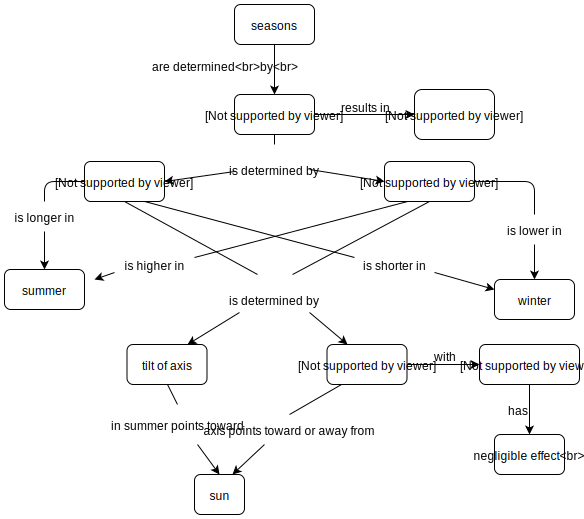
\includegraphics{../../files/seasons.pdf}

Concept Map for Seasons (from https://cmap.ihmc.us/)

To show how concept maps can be using in teaching programming, consider
this \texttt{for} loop in Python:

\begin{lstlisting}[language=python]
for letter in "abc":
    print(letter)
\end{lstlisting}

whose output is:

\begin{lstlisting}[backgroundcolor=\color{verylightgray}]
a
b
c
\end{lstlisting}

The three key ``things'' in this loop are shown in the top of
\protect\hyperlink{FIGURE}{f:memory-loop}, but they are only half the story. The
expanded version in the bottom shows the \emph{relationships} between those
things, which are as important for understanding as the concepts
themselves.

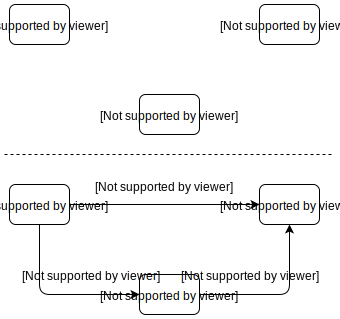
\includegraphics{../../files/for-loop.pdf}

Concept Map for a For Loop

Concept maps can be used in many ways:

\begin{description}
\tightlist
\item[Helping teachers figure out what they're trying to teach.]
Crucially, a concept map separates content from order: in our
experience, people rarely wind up teaching things in the order in
which they first drew them. (In technical terms, they reduce the
teacher's cognitive load---we will discuss this again in
\protect\hyperlink{CHAPTER}{s:load}.)
\item[Aiding communication between lesson designers.]
Teachers with very different ideas of what they're trying to teach
are likely to pull their learners in different directions; drawing
and sharing concept maps isn't guaranteed to prevent this, but it
helps.
\item[Aiding communication with learners.]
While it's possible to give learners a pre-drawn map at the start of
a lesson for them to annotate, it's better to draw it piece by piece
while teaching to reinforce the ties between what's in the map and
what the teacher said. (We will return to this idea in
\protect\hyperlink{SECTION}{s:load-split-attention}.)
\item[For assessment.]
Having learners draw pictures of what they think they just heard
shows the teacher what they missed and what was miscommunicated.
Reviewing learners' concept maps is too time-consuming to do as
in-class formative assessment, but very useful in weekly lectures
\emph{once learners are familiar with the technique}. The qualification
is necessary because any new way of doing things initially slows
people down---if a student is trying to make sense of basic
programming, asking them to figure out how to draw their thoughts at
the same time is an unfair load.
\end{description}

{[}\protect[\hyperlink{b:Kepp2008}{Kepp2008}]{]} looked at the use of concept mapping in computing
education. One of their findings was that, ``\ldots{}concept
mapping is troublesome for many students because it tests personal
understanding rather than knowledge that was merely learned by rote.'' As
someone who values understanding over rote knowledge, I count that as a
benefit.

Some teachers are also skeptical of whether novices can effectively map
their understanding, since introspection and explanation of
understanding are generally more advanced skills than understanding
itself. Like any other new tool or technique, concept maps have to be
taught and practiced if they are to be effective.

\begin{quote}\setlength{\parindent}{0pt}
\textbf{Start Anywhere}

When asked to draw their first concept map, many people will stare at
the blank page in front of them, not knowing where to start. When this
happens, write down two words associated with the topic you're trying
to map, then draw a line between them and add a label explaining how
those two ideas are related. You can then ask what other things are
related in the same way, what parts those things have, or what happens
before or after the concepts already on the page in order to discover
more nodes and arcs. After that, the hard part is often stopping.
\end{quote}

Concept maps are just one way to represent our understanding of a
subject; others include mind maps (which are usually radial and
hierarchical), conceptual diagrams (which use predefined categories and
relationships), and visual metaphors (which are striking images overlaid
with text) {[}\protect[\hyperlink{b:Eppl2006}{Eppl2006}]{]}. Maps, flowcharts, and blueprints can also
be useful in some contexts, as can decision trees like
{[}\protect[\hyperlink{b:Abel2009}{Abel2009}]{]} that shows how to choose the right kind of chart for
different kinds of questions and data.

What each does is \protect\hyperlink{g:externalized-cognition}{externalize cognition},
i.e., make thought processes and mental models visible so that they
can be compared, contrasted, and combined. {[}\protect[\hyperlink{b:Cher2007}{Cher2007}]{]}
suggests that externalizing cognition may be the main reason
developers draw diagrams when they are discussing things. They found
that most developers can't identify the parts of their own diagrams
shortly after having created them---instead of archiving information
for posterity, diagrams are actually a cache for short-term memory
that lets a participant in the discussion point at a wiggly bubble and
say ``that'' to trigger recall of several minutes of debate.

\begin{quote}\setlength{\parindent}{0pt}
\textbf{Rough Work and Honesty}

Many user interface designers believe that it's better to show people
rough sketches of their ideas rather than polished mock-ups because
people are more likely to give honest feedback on something that they
think only took a few minutes to create---if it looks as though what
they're critiquing took hours to create, most will pull their punches.
When drawing concept maps to motivate discussion, you should therefore
use pencils and scrap paper (or pens and a whiteboard) rather than
fancy computer drawing tools.
\end{quote}

\section{Seven Plus or Minus Two}\label{s:memory-seven-plus-or-minus}

While the graph model of knowledge is wrong but useful, another simple
model has a sounder physiological basis. As a rough approximation,
human memory can be divided into two distinct layers. The first,
called \protect\hyperlink{g:long-term-memory}{long-term} or \protect\hyperlink{g:persistent-memory}{persistent
memory}, is where we store things like our
friends' names, our home address, and what the clown did at our eighth
birthday party that scared us so much. It is essentially unbounded:
barring injury or disease, we will die before it fills up. However,
it is also slow to access---too slow to help us handle hungry lions
and disgruntled family members.

Evolution has therefore given us a second system called
\protect\hyperlink{g:short-term-memory}{short-term} or \protect\hyperlink{g:working-memory}{working
memory}. It is much faster, but also much smaller:
{[}\protect[\hyperlink{b:Mill1956}{Mill1956}]{]} estimated that the average adult's working memory
could only hold 7±2 items at a time. This is why \href{https://www.quora.com/Why-did-Bell-Labs-create-phone-numbers-of-7-digits-10-digits-Is-there-a-reason-that-dashes-and-brackets-are-used}{phone
numbers} are typically 7 or 8 digits long: back when
phones had dials instead of keypads, that was the longest string of
numbers most adults could remember accurately for as long as it took
the dial to go around several times. As \protect\hyperlink{SECTION}{s:memory-pattern}
discusses, short-term memory may actually be as small as 4±1 items;
our innate tendency to remember things together gives the illusion of
it being larger.

\begin{quote}\setlength{\parindent}{0pt}
\textbf{Participation}

The size of working memory is sometimes used to explain why sports
teams tend to have about half a dozen members or be broken down into
sub-groups like the forwards and backs in rugby. It is also used to
explain why meetings are only productive up to a certain number of
participants: if twenty people try to discuss something, either three
meetings are going on at once or half a dozen people are talking while
everyone else listens. The argument is that people's ability to keep
track of their peers is constrained by the size of working memory, but
so far as I know, the link has never been proven.
\end{quote}

7±2 is probably the most important number in programming. When
someone is trying to write the next line of a program, or understand
what's already there, they need to keep a bunch of arbitrary facts
straight in their head: what does this variable represent, what value
does it currently hold, etc. If the number of facts grows too large,
their mental model of the program comes crashing down (something we have
all experienced).

7±2 is also the most important number in teaching. A teacher cannot
push information directly into a learner's long-term memory. Instead,
whatever they present is first stored in the learner's short-term
memory, and is only transferred to long-term memory after it has been
held there and rehearsed (\protect\hyperlink{SECTION}{s:individual-strategies}). If the
teacher presents too much information too quickly, the new will
displace the old before it has a chance to consolidate in long-term
memory.

This is one of the reasons to create a concept map for a lesson when
designing it: doing so helps the teacher identify how many pieces of
separate information the learner will need to store in memory as the
lesson unfolds. In practice, I often draw a concept map, realize there's
far too much in it to teach in a single pass, and then carve out
tightly-connected subsections to break the lesson into digestible
pieces, each of which leads to a formative assessment.

\begin{quote}\setlength{\parindent}{0pt}
\textbf{Building Concept Maps Together}

Concept maps can be used as a classroom discussion exercise. Put
learners in small groups (2--4 people each), give each group some
sticky notes on which a few key concepts are written, and have them
build a concept map on a whiteboard by placing those sticky notes,
connecting them with labelled arcs, and adding any other concepts they
think they need.

The next time you have a team meeting, give everyone a sheet of paper
and have them spend a few minutes drawing a concept map of the project
you're all working on---separately. On the count of three, have everyone
reveal their concept maps simultaneously. Once everyone realizes how
different their mental models of the project are, a lot of interesting
discussion will ensue\ldots{}.
\end{quote}

The simple model of memory presented here has largely been replaced by a
more sophisticated one in which short-term memory is broken down into
several modal stores (e.g., for visual vs. linguistic memory), each of
which does some involuntary preprocessing {[}\protect[\hyperlink{b:Mill2016a}{Mill2016a}]{]}. Our
presentation is therefore an example of a mental model that aids
learning and everyday work, but is eventually superseded by something
more complicated.

Research also now indicates that the limiting factor for long-term
memory is not retention, but rather the ability to recall memories that
are present. Studying in short, spaced periods in a variety of contexts
improves recall; the reason may be that doing so creates more cues than
cramming (\protect\hyperlink{SECTION}{s:individual-strategies}).

\section{Pattern Recognition}\label{s:memory-pattern}

The preceding section said that short-term memory can only store
7±2 items at a time, and recent research have suggested that its
actual size might be as low as 4±1 items {[}\protect[\hyperlink{b:Dida2016}{Dida2016}]{]}. In
order to handle larger information sets, our minds create
\protect\hyperlink{g:chunking}{chunks}. For example, most of us remember words
as single items, rather than as sequences of letters. Similarly, the
pattern made by five spots on cards or dice is remembered as a whole
rather than as five separate pieces of information.

One key finding in cognition research is that experts have more and
larger chunks than non-experts, i.e., experts ``see'' larger patterns, and
have more patterns to match things against. This allows them to reason
at a higher level, and to search for information more quickly and more
accurately. However, chunking can also mislead us if we mis-identify
things: newcomers really can sometimes see things that experts have
looked at and missed.

Given how important chunking is to thinking, it is tempting to try to
teach patterns directly. One way to do this is to identify \href{https://en.wikipedia.org/wiki/Software_design_pattern}{design
patterns}, which are reusable solutions to common
problems. Patterns help competent practitioners think and talk to each
other in many domains (including teaching {[}\protect[\hyperlink{b:Berg2012}{Berg2012}]{]}), but
pattern catalogs are too dry and too abstract for novices to make
sense of on their own. That said, giving names to a small number of
patterns does seem to help with teaching, primarily by giving the
learners a richer vocabulary to think and communicate with
{[}\protect[\hyperlink{b:Kuit2004}{Kuit2004}],\protect[\hyperlink{b:Byck2005}{Byck2005}],\protect[\hyperlink{b:Saja2006}{Saja2006}]{]}. We will
return to this in \protect\hyperlink{SECTION}{s:pck-programming}.

\section{Becoming an Expert}\label{s:memory-becoming-expert}

So how does someone become an expert? The idea that ten thousand hours
of practice will do it is widely quoted but \href{http://www.goodlifeproject.com/podcast/anders-ericsson/}{probably not
true}: doing the same thing over and over again is
much more likely to solidify bad habits than improve performance. What
actually works is \protect\hyperlink{g:deliberate-practice}{deliberate practice} (also
sometimes called \protect\hyperlink{g:reflective-practice}{reflective practice}), which
is doing similar but subtly different things, paying attention to what
works and what doesn't, and then changing behavior in response to that
feedback to get cumulatively better.

A common progression is for people to go through three stages:

\begin{description}
\tightlist
\item[Act on feedback from others.]
For example, a student might write an essay about what they did on
their summer holiday and get feedback from a teacher telling them
how to improve it.
\item[Give feedback to others.]
For example, they might critique character development in \emph{The
Catcher in the Rye}. For this to be effective, it's essential that
they get feedback on their feedback, i.e., that the teacher critiques
their analysis.
\item[Give feedback to themselves.]
At some point, they start critiquing their own work in real time (or
nearly so) using the skills they have now built up. Doing this is so
much faster than waiting for feedback from others that proficiency
suddenly starts to take off.
\end{description}

\begin{quote}\setlength{\parindent}{0pt}
\textbf{What Counts as Deliberate Practice?}

{[}\protect[\hyperlink{b:Macn2014}{Macn2014}]{]} found that ``\ldots{}deliberate practice
explained 26\% of the variance in performance for games, 21\% for music,
18\% for sports, 4\% for education, and less than 1\% for professions.''
However, {[}\protect[\hyperlink{b:Eric2016}{Eric2016}]{]} critiqued this finding by saying, ``Summing
up every hour of any type of practice during an individual's career
implies that the impact of all types of practice activity on
performance is equal---an assumption that\ldots{}is inconsistent
with the evidence.'' To be effective, deliberate practice requires both
a clear performance goal and immediate informative feedback.
\end{quote}

\section{Exercises}\label{s:memory-exercises}

\subsection{Concept Mapping (pairs/30)}\label{concept-mapping-pairs30}

Draw a concept map for something you would teach in five minutes. Trade
with a partner, and critique each other's maps. Do they present concepts
or surface detail? Which of the relationships in your partner's map do
you consider concepts and vice versa?

\subsection{Concept Mapping (Again) (small groups/20)}\label{concept-mapping-again-small-groups20}

Working in groups of 3--4, have each person independently draw a concept
map showing their mental model of what goes on in a classroom. When
everyone is done, compare the concept maps. Which concepts and
relationships are common? Which are different? Where do your mental
models agree and disagree?

\subsection{A Concept Map for This Material (individual/30)}\label{a-concept-map-for-this-material-individual30}

After you have finished going through this material (not just this
chapter), pick one small topic, draw a concept map for it, and send it
to us (\protect\hyperlink{APPENDIX}{s:joining}). If we decide to add it to this book, we
will add you to the credits in the introduction.

\subsection{Noticing Your Blind Spot (small groups/10)}\label{noticing-your-blind-spot-small-groups10}

Consider all the things you have to know to understand this one line of
Python source code:

\begin{lstlisting}
answers = ['tuatara', 'tuataras', 'bus', "lick"]
\end{lstlisting}

As \href{https://twitter.com/elliewix/status/981285432922202113}{Elizabeth Wickes points out}:

\begin{itemize}
\item
  The square brackets surrounding the content mean we're working with
  a list (as opposed to square brackets immediately to the right of
  something, which is a data extraction notation).
\item
  The elements are separated by commas, which are outside/between the
  quotes (rather than inside, as they would be for quoted speech).
\item
  Each element is a character string, and we know that because of the
  quotes. We could have number or other data types in here if we
  wanted; we need quotes because we're working with strings.
\item
  We're mixing our use of single and double quotes, and Python doesn't
  care (so long as they balance around the individual strings).
\item
  Each comma is followed by a space, which is not required by Python,
  but we prefer it for readability.
\end{itemize}

Each of these details might be overlooked by an expert. Working in
groups of 3--4, select something equally short from a lesson you have
recently taught or taken and break it down to this level of detail.

\chapter{Cognitive Load}\label{s:load}

In {[}\protect[\hyperlink{b:Kirs2006}{Kirs2006}]{]}, Kirschner, Sweller and Clark wrote:

\begin{quote}\setlength{\parindent}{0pt}
Although unguided or minimally guided instructional approaches are
very popular and intuitively appealing\ldots{}these approaches
ignore both the structures that constitute human cognitive
architecture and evidence from empirical studies over the past
half-century that consistently indicate that minimally guided
instruction is less effective and less efficient than instructional
approaches that place a strong emphasis on guidance of the student
learning process. The advantage of guidance begins to recede only when
learners have sufficiently high prior knowledge to provide ``internal''
guidance.
\end{quote}

Their paper set off a minor academic storm, because beneath the jargon
the authors were claiming that allowing learners to ask their own
questions, set their own goals, and find their own path through a
subject, as they would when solving problems in real life, isn't
effective. This approach---called
\protect\hyperlink{g:inquiry-based-learning}{inquiry-based learning}---is
intuitively appealing, but the authors argued that it overloads learners
by requiring them to master a domain's factual content and its
problem-solving strategies at the same time.

More specifically, \protect\hyperlink{g:cognitive-load-theory}{cognitive load theory}
posited that people have to deal with three things when they're
learning:

\begin{description}
\tightlist
\item[Intrinsic load]
is what people have to keep in mind in order to absorb new material.
In a programming class, this might be understanding what a variable
is, or understanding how assignment in a programming language is
different from creating a reference to a cell in a spreadsheet.
Intrinsic load can't be reduced except by reducing the amount of
content being taught.
\item[Germane load]
is the (desirable) mental effort required to link new information to
old, which is one of the things that distinguishes learning from
memorization. An example might be remembering that a loop variable
is assigned a new value each time the loop executes.
\item[Extraneous load]
is everything else in the instructional material that distracts from
learning, such as matching the highlight colors in the instructor's
examples to the different color scheme used by the learner's own
editor.
\end{description}

Cognitive load theory holds that people have to split a fixed amount of
working memory between these three things. Our goal as instructors is to
maximize the memory available to handle germane load, which means
reducing the intrinsic load at each step and eliminating as much of the
extraneous load as possible.

For example, searching for a solution strategy is an extra burden on top
of actually applying that strategy. We can therefore accelerate learning
by giving learners worked examples that break a solution procedure down
into steps, each of which can be mastered on its own before being
combined with other steps (which is a step in its own right).

One way to do this is to give learners a series of
\protect\hyperlink{g:faded-example}{faded examples}. The first example
presents a nearly-complete use of the same problem-solving strategy just
demonstrated, but with a small number of blanks for the learner to fill
in. The next problem is of the same type, but has more blanks, and so on
until the learner is asked to solve the entire problem. The material
that \emph{isn't} blank is often referred to as
\protect\hyperlink{g:scaffolding}{scaffolding}, since it serves the same
purpose as the scaffolding set up temporarily at a building site.

Faded examples can be used in almost every kind of teaching, from sport
and music to contract law. Someone teaching programming might use them
by first explaining how to calculate the total length of a list of
words:

\begin{lstlisting}
# total_length(["red", "green", "blue"]) => 12
define total_length(list_of_words):
    total = 0
    for each word in list_of_words:
        total = total + word.length()
    return total
\end{lstlisting}

and then asking learners to fill in the blanks in this (which focuses
their attention on control structures):

\begin{lstlisting}
# word_lengths(["red", "green", "blue"]) => [3, 5, 4]
define word_lengths(list_of_words):
    list_of_lengths = []
    for each ____ in ____:
        list_of_lengths.append(____)
    return list_of_lengths
\end{lstlisting}

The next problem might be this (which focuses their attention on
updating the final result):

\begin{lstlisting}
# join_all(["red", "green", "blue"]) => "redgreenblue"
define join_all(list_of_words):
    joined_words = ____
    for each ____ in ____:
        ____
    return joined_words
\end{lstlisting}

Learners would finally be asked to write an entire function on their
own:

\begin{lstlisting}
# make_acronym(["red", "green", "blue"]) => "RGB"
define make_acronym(list_of_words):
    ____
\end{lstlisting}

Faded examples work because they introduce the problem-solving strategy
piece by piece: at each step, learners have one new problem to tackle,
which is less intimidating than a blank screen or a blank sheet of paper
(\protect\hyperlink{SECTION}{s:classroom-practices}). It also encourages learners to
think about the similarities and differences between various approaches,
which helps create the linkages in their mental models that help
retrieval.

\begin{quote}\setlength{\parindent}{0pt}
\textbf{Efficiency vs. Extent}

Seeing worked examples accelerates learning more than having students
write lots of code themselves {[}\protect[\hyperlink{b:Skud2014}{Skud2014}]{]}. As we will see in
\protect\hyperlink{CHAPTER}{s:pck}, deconstructing code by tracing it or debugging it
also increases the efficiency of learning {[}\protect[\hyperlink{b:Grif2016}{Grif2016}]{]}. However,
this isn't the same as saying that people learn more unless they see
additional problems.
\end{quote}

The key to constructing a good faded example is to think about the
problem-solving strategy it is meant to teach. For example, the series
of problems are all examples of the \emph{accumulator pattern}, in which the
results of processing items from a collection are repeatedly added to a
single variable in some way to create the final result.

Critics have sometimes argued that any result can be justified after the
fact by labelling things that hurt performance as extraneous load and
things that don't as intrinsic or germane. However, instruction based on
cognitive load theory is undeniably effective. For example,
{[}\protect[\hyperlink{b:Maso2016}{Maso2016}]{]} redesigned a database course to remove split
attention and redundancy effects, and provide worked examples and
sub-goals. The new course reduced exam failure rate by 34\% on an
identical final exam and increased student satisfaction.

A decade after the publication of {[}\protect[\hyperlink{b:Kirs2006}{Kirs2006}]{]}, a growing number
of people believe that cognitive load theory and inquiry-based
approaches are compatible if viewed in the right way. {[}\protect[\hyperlink{b:Kaly2015}{Kaly2015}]{]}
argues that cognitive load theory is basically micro-management of
learning within a broader context that considers things like motivation,
while {[}\protect[\hyperlink{b:Kirs2018}{Kirs2018}]{]} extends cognitive load theory to include
collaborative aspects of learning. As with {[}\protect[\hyperlink{b:Mark2018}{Mark2018}]{]} (discussed
in \protect\hyperlink{SECTION}{s:individual-strategies}), researchers' perspectives may
differ, but the practical implementation of their theories often wind up
being the same.

\begin{quote}\setlength{\parindent}{0pt}
\textbf{Cognitive Apprenticeship}

An alternative model of learning and instruction that also uses
scaffolding and fading is
\protect\hyperlink{g:cognitive-apprenticeship}{cognitive apprenticeship},
which emphasizes the way in which a master passes on skills and
insights to an apprentice. The master provides models of performance
and outcomes, then coaches novices as they take their first steps by
explaining what they're doing and why {[}\protect[\hyperlink{b:Coll1991}{Coll1991}],\protect[\hyperlink{b:Casp2007}{Casp2007}]{]}. The
apprentice reflects on their own problem solving, e.g., by thinking
aloud or critiquing their own work, and eventually explores problems
of their own choosing.

This model tells us that instructors should present several examples
when presenting a new idea so that learners can see what to
generalize, and that we should vary the form of the problem to make it
clear what are and aren't superficial features. (For a long time, I
believed that the variable holding the value a function was going to
return \emph{had} to be called \texttt{result} because my instructor always used
that name in examples.) Problems should be presented in real-world
contexts, and we should encourage self-explanation, since it helps
learners organize and make sense of what they have just been taught.
This is discussed in more detail in
\protect\hyperlink{SECTION}{s:individual-strategies}.
\end{quote}

\subsection{Parsons Problems}\label{parsons-problems}

Another kind of exercise that can be explained in terms of cognitive
load theory is called a \protect\hyperlink{g:parsons-problem}{Parsons Problem}
(named after one of their creators {[}\protect[\hyperlink{b:Pars2006}{Pars2006}]{]}). If you are
teaching someone to speak a new language, you could ask them a question,
and then give them the words they need to answer the question, but in
jumbled order. Their task is to put the words in the right order to
answer the question grammatically, which frees them from having to think
simultaneously about what to say \emph{and} how to say it.

Similarly, when teaching people to program, you can give them the lines
of code they need to solve a problem, and ask them to put them in the
right order. This allows them to concentrate on control flow and data
dependencies, i.e., on what has to happen before what, without being
distracted by variable naming or trying to remember what functions to
call. Multiple studies have shown that Parsons Problems take less time
for learners to do, but produce equivalent educational outcomes
{[}\protect[\hyperlink{b:Eric2017}{Eric2017}]{]}.

\subsection{Labelled Subgoals}\label{labelled-subgoals}

\protect\hyperlink{g:subgoal-labelling}{Subgoal labelling} means giving names
to the steps in a step-by-step description of a problem-solving process.
{[}\protect[\hyperlink{b:Marg2016}{Marg2016}],\protect[\hyperlink{b:Morr2016}{Morr2016}]{]} all found that students with labelled
subgoals solved Parsons Problems better than students without, and the
same benefit is seen in other problem domains {[}\protect[\hyperlink{b:Marg2012}{Marg2012}]{]}.
Returning to the Python example used earlier, the subgoals in finding
the total length of a list of words or constructing an acronym are:

\begin{enumerate}
\item
  Create an empty value of the type to be returned.
\item
  Get the value to be added to the result from the loop variable.
\item
  Update the result with that value.
\end{enumerate}

Labelling subgoals works because grouping related steps in a chunk
(\protect\hyperlink{SECTION}{s:memory-pattern}) and giving each chunk a name helps
learners distinguish between generic information and information that is
specific to the problem at hand, which reduces cognitive load. It also
helps them build a mental model of that kind of problem, so that they
can solve other problems of that kind, and gives them a natural
opportunity for self-explanation (\protect\hyperlink{SECTION}{s:individual-strategies}).

\section{Split Attention}\label{s:load-split-attention}

Research by Mayer and colleagues on the
\protect\hyperlink{g:split-attention-effect}{split-attention effect} is
closely related to cognitive load theory {[}\protect[\hyperlink{b:Maye2003}{Maye2003}]{]}. Linguistic
and visual input are processed by different parts of the human brain,
and linguistic and visual memories are stored separately as well. This
means that correlating linguistic and visual streams of information
takes cognitive effort: when someone reads something while hearing it
spoken aloud, their brain can't help but check that it's getting the
same information on both channels (a topic we'll return to when
discussing dual coding in \protect\hyperlink{SECTION}{s:individual-strategies}).

Learning is therefore more effective when information is presented
simultaneously in two different channels, but when that information is
complementary rather than redundant. For example, people generally find
it harder to learn from a video that has both narration and on-screen
captions than from one that has either the narration or the captions but
not both, because some of their attention has to be devoted to checking
that the narration and the captions agree with each other. Two notable
exceptions to this are people who do not yet speak the language well and
people with hearing exercises or other special needs, both of whom may
find that the extra effort is a net benefit.

This explains why it's more effective to draw a diagram piece by piece
while teaching rather than to present the whole thing at once. If parts
of the diagram appear at the same time as things are being said, the two
will be correlated in the learner's memory. Pointing at part of the
diagram later is then more likely to trigger recall of what was being
said when that part was being drawn.

The split-attention effect does \emph{not} mean that learners shouldn't try
to reconcile multiple incoming streams of information---after all, this is
something they have to do in the real world {[}\protect[\hyperlink{b:Atki2000}{Atki2000}]{]}. Instead,
it means that instruction shouldn't require it while people are
mastering unit skills; instead, using multiple sources of information
simultaneously should be treated as a separate learning task.

\begin{quote}\setlength{\parindent}{0pt}
\textbf{Not All Graphics Are Created Equal}

{[}\protect[\hyperlink{b:Sung2012}{Sung2012}]{]} presents an elegant study that distinguishes
\emph{seductive} graphics (which are highly interesting but not directly
relevant to the instructional goal), \emph{decorative} graphics (which are
neutral but not directly relevant to the instructional goal), and
\emph{instructive} graphics (directly relevant to the instructional goal).
Students who received any kind of graphic gave significantly higher
satisfaction ratings to material than those who didn't get graphics,
but only students who got instructive graphics actually performed
better.

Similarly, {[}\protect[\hyperlink{b:Stam2013}{Stam2013}],\protect[\hyperlink{b:Stam2014}{Stam2014}]{]} found that having more
information can actually lower performance. They showed children
pictures, pictures and numbers, or just numbers for two tasks:
fraction equivalence and fraction addition. For equivalence, having
pictures or pictures and numbers outperformed having numbers only. For
addition, however, having pictures outperformed pictures and numbers,
which outperformed just having numbers.
\end{quote}

\section{Minimal Manuals}\label{s:load-minimal}

The most extreme use of cognitive load theory may be the ``minimal
manual'' method introduced in {[}\protect[\hyperlink{b:Carr1987}{Carr1987}]{]}. Its starting point is
a quote from a user: ``I want to do something, not learn how to do
everything.'' Carroll and colleagues therefore redesigned training to
present every idea as a single-page self-contained task: a title
describing what the page was about, step-by-step instructions of how to
do something really simple (like how to delete a blank line in a text
editor), and then several notes how to recognize and debug common
problems.

Carroll and colleagues found that rewriting training materials this way
made them shorter overall, and that people using them learned faster.
Later studies like {[}\protect[\hyperlink{b:Lazo1993}{Lazo1993}]{]} confirmed that this approach
outperformed the traditional approach regardless of prior experience
with computers.

Looking back, {[}\protect[\hyperlink{b:Carr2014}{Carr2014}]{]} summarized this work by saying:

\begin{quote}\setlength{\parindent}{0pt}
Our ``minimalist'' designs sought to leverage user initiative and prior
knowledge, instead of controlling it through warnings and ordered
steps. It emphasized that users typically bring much expertise and
insight to this learning, for example, knowledge about the task
domain, and that such knowledge could be a resource to instructional
designers. Minimalism leveraged episodes of error recognition,
diagnosis, and recovery, instead of attempting to merely forestall
error. It framed troubleshooting and recovery as learning
opportunities instead of as aberrations.
\end{quote}

He goes on to say that at the time, instruction decomposed skills into
sub-skills hierarchically and then drilled people on the sub-skills.
However, this meant context was lost: the goals weren't apparent until
people had learned the pieces. Since people want to dive in and do real
tasks, well-designed instruction should help them do that.

\section{Exercises}\label{s:load-exercises}

\subsection{Create a Faded Example (pairs/30)}\label{create-a-faded-example-pairs30}

It's very common for programs to count how many things fall into
different categories: for example, how many times different colors
appear in an image, or how many times different words appear in a
paragraph of text.

\begin{enumerate}
\item
  Create a short example (no more than 10 lines of code) that shows
  people how to do this, and then create a second example that solves
  a similar problem in a similar way, but has a couple of blanks for
  learners to fill in. How did you decide what to fade out? What would
  the next example in the series be?
\item
  Define the audience for your examples. For example, are these
  beginners who only know some basics programming concepts? Or are
  these learners with some experience in programming but not in
  Python?
\item
  Show your example to a partner, but do \emph{not} tell them what level it
  is intended for. Once they have filled in the blanks, ask them what
  level they think it is for.
\end{enumerate}

If there are people among the trainees who don't program at all, try to
place them in different groups, and have them play the part of learners
for those groups. Alternatively, choose a different problem domain and
develop a faded example for it.

\subsection{Classifying Load (small groups/15)}\label{classifying-load-small-groups15}

Working in groups of 3--4, choose a short lesson that one of you has
taught or taken recently, make a point-form list of the ideas,
instructions, and explanations it contains, and then classify each as
intrinsic, germane, or extraneous. (The exercise ``Noticing Your Blind
Spot'' in \protect\hyperlink{SECTION}{s:memory-exercises} will give you an idea of how
detailed your point-form list should be.)

\subsection{Create a Parsons Problem (pairs/20)}\label{create-a-parsons-problem-pairs20}

Write five or six lines of code that does something useful, jumble them,
and ask your partner to put them in order. If you are using an
indentation-based language like Python, do not indent any of the lines;
if you are using a curly-brace language like Java, do not include any of
the curly braces. Again, if your group includes people who aren't
programmers, try using a different problem domain, such as making
guacamole.

\subsection{Minimal Manuals (individual/20)}\label{minimal-manuals-individual20}

Write a one-page guide to doing something simple that your learners
might encounter in one of your classes, such as centering text
horizontally or printing a number with a certain number of digits after
the decimal points. Try to list at least three or four incorrect
behaviors or outcomes the learner might see, and include a one- or
two-line explanation of why each happens and how to correct it (i.e., go
from symptoms to cause to fix).

\subsection{Cognitive Apprenticeship (pairs/15)}\label{cognitive-apprenticeship-pairs15}

Pick a small coding problem (something you can do in two or three
minutes) and think aloud as you work through it while your partner asks
questions about what you're doing and why. As you work, do not just
comment on what you're doing, but also on why you're doing it, how you
know it's the right thing to do, and what alternatives you've considered
but discarded. When you are done, swap roles with your partner and
repeat the exercise.

\subsection{Critiquing Graphics (individual/30)}\label{critiquing-graphics-individual30}

{[}\protect[\hyperlink{b:Maye2009}{Maye2009}]{]} presents six principles for designing good diagrams
for teaching. As summarized in {[}\protect[\hyperlink{b:Mill2016a}{Mill2016a}]{]}, they are:

\begin{description}
\tightlist
\item[Signalling:]
visually highlight the most important points that you want students
to retain so that they stand out from less-critical material.
\item[Spatial contiguity:]
if using captions or other text to accompany graphics, place them as
close to the graphics as practical to offset the cost of shifting
between the two. If using diagrams or animations, place captions
right next to relative components instead of putting them in one big
block of text.
\item[Temporal contiguity:]
present spoken narration and graphics as close in time as
practical---presenting both at once is better than presenting them
one after another.
\item[Segmenting:]
when presenting a long sequence of material or when students are
inexperienced with the subject, break up the presentation into
shorter segments and let students control how quickly they advance
from one part to the next.
\item[Pretraining:]
if students don't know the major concepts and terminology used in
your presentation, set up a module just to teach those concepts and
terms and make sure they complete that module beforehand.
\item[Modality:]
students learn better from pictures plus audio narration than from
pictures plus text, unless there are technical words or symbols, or
the students are non-native speakers.
\end{description}

Choose a video of a lesson or talk online that uses slides or other
static presentations, and rate its graphics as ``poor'', ``average'', or
``good'' according to these six criteria.

\chapter{Individual Learning}\label{s:individual}

The previous three chapters have looked at what instructors can do to
help their learners. This chapter looks at what learners can do for
themselves by changing their study strategies and getting enough rest.

The key to getting more out of learning is
\protect\hyperlink{g:metacognition}{metacognition}, or thinking about one's
own thinking processes. Just as good musicians listen to their own
playing, and good teachers reflect on their teaching
(\protect\hyperlink{CHAPTER}{s:performance}), learners will learn better and faster if
they make plans, set goals, and monitor their progress. It's difficult
for learners to master these skills in the abstract---for example, just
telling them to make plans doesn't have any effect---but lessons can be
designed to encourage certain study practices, and drawing attention to
these practices in class helps them realize that learning is a skill
that can be improved like any other {[}\protect[\hyperlink{b:McGu2015}{McGu2015}],\protect[\hyperlink{b:Miya2018}{Miya2018}]{]}.

The big prize is transfer of learning, which occurs when one thing we
have learned helps us learn something else more quickly. Researchers
distinguish between \protect\hyperlink{g:near-transfer}{near transfer}, which occurs
between similar or related areas like fractions and decimals, or loops
in different programming languages, and \protect\hyperlink{g:far-transfer}{far
transfer}, which occurs between dissimilar
domains---the idea that learning to play chess will help mathematical
reasoning or vice versa.

Near transfer undoubtedly occurs---no kind of learning beyond simple
memorization could occur if it didn't---and instructors leverage it all
the time by giving learners exercises that are close in form or content
to what has just been presented in a lesson. However, {[}\protect[\hyperlink{b:Sala2017}{Sala2017}]{]}
recently analyzed many studies of far transfer and concluded that while
we might \emph{want} to believe in it:

\begin{quote}\setlength{\parindent}{0pt}
\ldots{}the results show small to moderate effects. However, the
effect sizes are inversely related to the quality of the experimental
design\ldots{} We conclude that far transfer of learning rarely
occurs.
\end{quote}

When far transfer \emph{does} occur, it seems to happen only once a subject
has been mastered {[}\protect[\hyperlink{b:Gick1987}{Gick1987}]{]}. In practice, this means that
learning to program won't help you play chess and vice versa.

\section{Six Strategies}\label{s:individual-strategies}

Psychologists study learning in a wide variety of ways, but have
reached similar conclusions about what actually works
{[}\protect[\hyperlink{b:Mark2018}{Mark2018}]{]}. The \href{http://www.learningscientists.org/}{Learning Scientists}
have catalogued six of these strategies and summarized them in \href{http://www.learningscientists.org/downloadable-materials}{a set
of downloadable posters}. Teaching
these strategies to students, and mentioning them by name when you use
them in class, can help them learn how to learn faster and better
{[}\protect[\hyperlink{b:Wein2018}{Wein2018}]{]}.

\subsection{Spaced Practice}\label{spaced-practice}

Ten hours of study spread out over five days is more effective than two
five-hour days, and far better than one ten-hour day. You should
therefore create a study schedule that spreads study activities over
time: block off at least half an hour to study each topic each day
rather than trying to cram everything in the night before an exam
{[}\protect[\hyperlink{b:Kang2016}{Kang2016}]{]}.

You should also review material after each class (but not immediately
after---take at least a half-hour break). When reviewing, be sure to
include at least a little bit of older material: for example, spend 20
minutes looking over notes from that day's class, and then 5 minutes
each looking over material from the previous day and from a week before.
(Doing this also helps you catch any gaps or mistakes in previous sets
of notes while there's still time to correct them or ask questions: it's
painful to realize the night before the exam that you have no idea why
you underlined ``Demodulate!!'' three times.)

When reviewing, make notes about things that you had forgotten: for
example, make a flash card for each fact that you couldn't remember, or
that you remembered incorrectly. This will help you focus the next round
of study on things that most need attention.

\begin{quote}\setlength{\parindent}{0pt}
\textbf{The Value of Lectures}

According to {[}\protect[\hyperlink{b:Mill2016a}{Mill2016a}]{]}, ``The lectures that predominate in
face-to-face courses are relatively ineffective ways to teach, but
they probably contribute to spacing material over time, because they
unfold in a set schedule over time. In contrast, depending on how the
courses are set up, online students can sometimes avoid exposure to
material altogether until an assignment is nigh.''
\end{quote}

\subsection{Retrieval Practice}\label{retrieval-practice}

Researchers now believe that the limiting factor for long-term memory is
not retention (what is stored), but recall (what can be accessed).
Recall of specific information improves with practice, so outcomes in
real situations can be improved by taking practice tests or summarizing
the details of a topic from memory and then checking what was and wasn't
remembered. For example, {[}\protect[\hyperlink{b:Karp2008}{Karp2008}]{]} found that repeated testing
improved recall of word lists from 35\% to 80\%.

Research also shows that recall is better when practice uses
activities similar to those used in testing; for example, writing
personal journal entries helps with multiple-choice quizzes, but less
than doing multiple-choice quizzes {[}\protect[\hyperlink{b:Mill2016a}{Mill2016a}]{]}. This is
called \protect\hyperlink{g:transfer-appropriate-processing}{transfer-appropriate
processing}.

One way to exercise retrieval skills is to solve problems twice. The
first time, do it entirely from memory without notes or discussion with
peers. After grading your own work against a rubric supplied by the
instructor, solve the problem again using whatever resources you want.
The difference between the two shows you how well you were able to
retrieve and apply knowledge.

Another method (mentioned above) is to create flash cards. In physical
form, a question or other prompt is written on one side, and the answer
is written on the other; in digital form, these are ideal for deployment
on mobile devices like phones. If you are studying as part of a group,
you can exchange flash cards with a partner; this also helps you
discover important ideas that you may have missed or misunderstood.

A quicker version of this is
\protect\hyperlink{g:read-cover-retrieve}{read-cover-retrieve}: as you read something,
cover up key terms or sections with small sticky notes. When you are
done, go through it a second time and see how well you can guess
what's under each of those stickies.

Whatever method you use, don't just practice recalling facts and
definitions: make sure you also check your understanding of big ideas
and the connections between them. Sketching a concept map and then
comparing it to your notes or to a previously-drawn concept map is a
quick way to do this.

\begin{quote}\setlength{\parindent}{0pt}
\textbf{Hypercorrection}

One powerful finding in learning research is the \protect\hyperlink{g:hypercorrection}{hypercorrection
effect} {[}\protect[\hyperlink{b:Metc2016}{Metc2016}]{]}. Most people don't
like to be told they're wrong, so it's reasonable to assume that the
more confident someone is that the answer they've given in a test is
correct, the harder it is to change their mind if they were actually
wrong. However, it turns out that the opposite is true: the more
confident someone is that they were right, the more likely they are
not to repeat the error if they are corrected.
\end{quote}

\subsection{Interleaving}\label{interleaving}

One way you can space your practice is to interleave study of different
topics: instead of mastering one subject, then the next, then a third,
shuffle study sessions. Even better, switch up the order: A-B-C-B-A-C is
better than A-B-C-A-B-C, which in turn is better than A-A-B-B-C-C
{[}\protect[\hyperlink{b:Rohrer2015}{Rohrer2015}]{]}. This is effective because interleaving fosters
creation of more links between different topics, which in turn increases
retention and recall.

How long you should spend on each item depends on the subject and how
well you know it, but somewhere between 10 and 30 minutes is long enough
for you to get into a state of flow (\protect\hyperlink{SECTION}{s:individual-time}) but
not for your mind to wander. Interleaving study will initially feel
harder than focusing on one topic at a time, but that's a sign that it's
working. If you are making flash cards for yourself, or doing practice
tests, you should see improvement after only a couple of days.

\subsection{Elaboration}\label{elaboration}

Explaining things to yourself as you go through them helps you
understand and remember them. One way to do this is to follow up each
answer on a practice quiz with an explanation of why that answer is
correct, or conversely with an explanation of why some other plausible
answer isn't. Another is to tell yourself how a new idea is similar to
or different from one that you have seen previously.

Talking to yourself may seem like an odd way to study, but
{[}\protect[\hyperlink{b:Biel1995}{Biel1995}]{]} explicitly trained people in self-explanation, and
yes, they outperformed those who hadn't been trained. An exercise that
builds on this is to go through code line by line with a group, having a
different person to explain each line in turn and say why it is there
and what it accomplishes.

{[}\protect[\hyperlink{b:Chi1989}{Chi1989}]{]} found that some learners simply halt when they hit an
unexplained step (or a step whose explanation they don't understand)
when doing mechanics problems in a physics class. Others who pause their
``execution'' of the example to generate an explanation of what's going on
learn faster. Instructors should therefore demonstrate the latter
strategy to learners.

Explaining things to others even works on exams, though the extent of
the benefits are still being
studied. {[}\protect[\hyperlink{b:Cao2017a}{Cao2017a}],\protect[\hyperlink{b:Cao2017b}{Cao2017b}]{]} looked at two-stage
exams, i.e., a normal (individual) exam which is then immediately
followed by a second exam in which students work in small groups to
solve a set of problems. They found significant short-term gains for
students doing exams collaboratively, but not long-term gains, i.e.,
the benefits visible a couple of weeks after the mid-term had faded by
the final. They also found that students in the middle of the class
benefited strongly, and that homogeneous-ability groups benefited,
while heterogeneous groups did not.

\subsection{Concrete Examples}\label{concrete-examples}

One specific form of elaboration is so useful that it deserves its own
heading, and that is the use of concrete examples. Whenever you have a
statement of a general principle, try to provide one or more examples of
its use, or conversely take each particular problem and list the general
principles it embodies. {[}\protect[\hyperlink{b:Raws2014}{Raws2014}]{]} found that interleaving
examples and definitions made it more likely that learners would
remember the latter correctly.

One structured way to do this is the \href{https://betterexplained.com/articles/adept-method/}{ADEPT method}: give an
\textbf{A}nalogy, draw a \textbf{D}iagram, present an \textbf{E}xample, describe the
idea in \textbf{P}lain language, and then give the \textbf{T}echnical details.
Again, if you are studying with a partner or in a group, you can swap
and check work: see if you agree that other people's examples actually
embody the principle being discussed, or which principles are used in
an example that they haven't listed.

Another useful technique is to teach by contrast, i.e., to show learners
what a solution is \emph{not}, or what kind of problem a technique \emph{won't}
solve. For example, when showing children how to simplify fractions,
it's important to give them a few like 5/7 that can't be simplified so
that they don't become frustrated looking for answers that don't exist.

\subsection{Dual Coding}\label{dual-coding}

The last of the six core strategies that the \href{http://www.learningscientists.org/}{Learning
Scientists} describe is to present words and
images together. As discussed in \protect\hyperlink{SECTION}{s:load-split-attention},
different subsystems in our brains handle and store linguistic and
visual information, and if complementary information is presented
through both channels, then they can reinforce one another. However,
learning is more effective when the same information is \emph{not}
presented simultaneously in two different channels
{[}\protect[\hyperlink{b:Maye2003}{Maye2003}]{]}, because then the brain has to expend effort to
check the channels against each other.

One way to take advantage of dual coding is to draw or label timelines,
maps, family trees, or whatever else seems appropriate to the material.
(I am personally fond of pictures showing which functions call which
other functions in a program.) Drawing a diagram \emph{without} labels, then
coming back later to label it, is excellent retrieval practice.

\section{Time Management}\label{s:individual-time}

I used to brag about the hours I was working. Not in so many words, of
course---I had \emph{some} social skills---but I would show up for class around
noon, unshaven and yawning, and casually mention how I'd been up working
`til 6:00 a.m.

Looking back, I can't remember who I was trying to impress. Instead,
what I remember is how much of the work I did in those all-nighters I
threw away once I'd had some sleep, and how much damage the stuff I
didn't throw away did to my grades.

My mistake was to confuse ``working'' with ``being productive''. You can't
produce software (or anything else) without doing some work, but you can
easily do lots of work without producing anything of value. Convincing
people of this can be hard, especially when they're in their teens or
twenties, but pays tremendous dividends.

Scientific study of overwork and sleep deprivation goes back to at least
the 1890s (see {[}\protect[\hyperlink{b:Robi2005}{Robi2005}]{]} for a short, readable summary). The
most important results for learners are:

\begin{enumerate}
\item
  Working more than eight hours a day for an extended period of time
  lowers your total productivity, not just your hourly
  productivity---i.e., you get less done in total (not just per hour)
  when you're in crunch mode than you do when you work regular hours.
\item
  Working over 21 hours in a stretch increases the odds of you making
  a catastrophic error just as much as being legally drunk.
\item
  Productivity varies over the course of the workday, with the
  greatest productivity occurring in the first four to six hours.
  After enough hours, productivity approaches zero; eventually it
  becomes negative.
\end{enumerate}

These facts have been reproduced and verified for over a century, and
the data behind them is as solid as the data linking smoking to lung
cancer. The catch is that \emph{people usually don't notice their abilities
declining}. Just like drunks who think they're still able to drive,
people who are deprived of sleep don't realize that they're not
finishing their sentences (or thoughts). Five eight-hour days per week
has been proven to maximize long-term total output in every industry
that has ever been studied; studying or programming are no different.

But what about short bursts now and then, like pulling an all-nighter to
meet a deadline? That has been studied too, and the results aren't
pleasant. Your ability to think drops by 25\% for each 24 hours you're
awake. Put it another way, the average person's IQ is only 75 after one
all-nighter, which puts them in the bottom 5\% of the population. Two all
nighters in a row, and their effective IQ is 50, which is the level at
which people are usually judged incapable of independent living.

\begin{quote}\setlength{\parindent}{0pt}
\textbf{When You Just Can't Say No}

Research has shown that our ability to exert willpower runs out,
just like our ability to use muscles: if we have to resist eating
the last donut on the tray when we're hungry, we are less likely to
fold laundry and vice versa. This is called \protect\hyperlink{g:ego-depletion}{ego
depletion} {[}\protect[\hyperlink{b:Mill2016a}{Mill2016a}]{]}, and an effective
counter is to build up habits so that doing the right thing is
automatic.
\end{quote}

``But---but---we have so many assignments to do!'', your learners say. ``And
they're all due at once! We \emph{have} to work extra hours to get them all
done!'' No: in order to be productive, they have to prioritize and
focus, and in order to do that, they have to be taught how. One
widely-used technique is to make a list of things that need to be done,
sort them by priority, and then switch off email and other interruptions
for 30-60 minutes and complete one of those tasks. If any task on a
to-do list is more than an hour long, break it down into smaller pieces
and prioritize those separately.

The most important part of this is switching off
interruptions. Despite what many people want to believe, people are
not good at multi-tasking. What we can become good at is
\protect\hyperlink{g:automaticity}{automaticity}, which is the ability to do something
routine in the background while doing something else
{[}\protect[\hyperlink{b:Mill2016a}{Mill2016a}]{]}. Most of us can talk while chopping onions, or
drink coffee while reading; with practice, we can also take notes
while listening, but we can't study effectively, program, or do other
mentally challenging tasks while paying attention to something else.

The point of all this organization and preparation is to get into the
most productive mental state possible. Psychologists call it
\protect\hyperlink{g:flow}{flow} {[}\protect[\hyperlink{b:Csik2008}{Csik2008}]{]}; athletes call it ``being in the
zone'', while musicians talk about losing themselves in what they're
playing. Whatever name you use, people produce much more per unit of
time in this state than normal.

That's the good news. The bad news is that it takes roughly ten minutes
to get back into a state of flow after an interruption, no matter how
short the interruption was. This means that if you are interrupted half
a dozen times per hour, you are \emph{never} at your productive peak.

\section{Peer Assessment}\label{s:individual-peer}

Asking people on a team to rate their peers is a common practice in
industry. {[}\protect[\hyperlink{b:Sond2012}{Sond2012}]{]} surveyed the literature on student peer
assessment, distinguishing between grading and reviewing. The benefits
they found included increasing the amount, diversity, and timeliness of
feedback, helping students exercise higher-level thinking, encouraging
reflective practice, and supporting development of social skills. The
concerns were predictable: validity and reliability, motivation and
procrastination, trolls, collusion, and plagiarism. However, while these
concerns are legitimate, the evidence shows that they aren't significant
in class. For example, {[}\protect[\hyperlink{b:Kauf2000}{Kauf2000}]{]} compared confidential peer
ratings and grades on several axes for two undergraduate engineering
courses and found that self-rating and peer ratings statistically
agreed, that collusion (i.e., everyone giving their peers the same
grades) wasn't significant, that students didn't inflate their
self-ratings, and crucially, that ratings were not biased by gender or
race.

One important variation on peer assessment and review is \protect\hyperlink{g:contributing-student}{contributing
student pedagogy}, in which students produce
artifacts to contribute to other students' learning. This can be
developing a short lesson and sharing it with the class, adding to a
question bank, or writing up notes from a particular lecture for
in-class publication. For example, {[}\protect[\hyperlink{b:Fran2018}{Fran2018}]{]} found that
students who made short videos to teach concepts to their peers had a
significant increase in their own learning compared to those who only
studied the material or viewed the videos.

Another is \protect\hyperlink{g:calibrated-peer-review}{calibrated peer review}, in
which a student reviews one or more examples using a rubric and
compares their evaluation against the instructor's review of the same
work {[}\protect[\hyperlink{b:Kulk2013}{Kulk2013}]{]}. Only once student's evaluations are close
enough to the instructor's are they allowed to start evaluating peers'
actual work.

As long as evaluation is based on observables, rather than personality
traits, peer assessment can actually be as accurate as assessment by TAs
and other outsiders. ``Observables'' means that instead of asking, ``Is the
person outgoing,'' or ``Does the person have a positive attitude,''
assessments should ask, ``Does the person listen attentively during
meetings,'' or, ``Does the person attempt to solve problems before asking
for help.'' The evaluation form in \protect\hyperlink{APPENDIX}{s:peereval} shows a
sample to get you started. To use it, rank yourself and each of your
teammates, then calculate and compare scores.

\section{Exercises}\label{s:individual-exercises}

\subsection{Learning Strategies (individual/20)}\label{learning-strategies-individual20}

\begin{enumerate}
\item
  Which of the six learning strategies do you regularly use? Which
  ones do you not?
\item
  Write down three general concepts that you want your learners to
  master, and then give two specific examples of each. (This uses the
  ``concrete examples'' practice).
\item
  For each of those concepts, work backward from one of your examples
  to explain how the concept explains it. (This uses the ``elaboration''
  practice).
\end{enumerate}

\subsection{Connecting Ideas (pairs/5)}\label{connecting-ideas-pairs5}

This exercise is an example of using elaboration to improve
retention. Pick a partner, and have each person independently choose an
idea, then announce your ideas and try to find a four-link chain that
leads from one to the other. For example, if the two ideas are
``Saskatchewan'' and ``statistics'', the links might be:

\begin{itemize}
\item
  Saskatchewan is a province of Canada;
\item
  Canada is a country;
\item
  countries have governments;
\item
  governments are elected; and
\item
  people try to predict election results using statistics
\end{itemize}

\subsection{Convergent Evolution (pairs/15)}\label{convergent-evolution-pairs15}

One practice that wasn't covered above is \protect\hyperlink{g:guided-notes}{guided
notes}, which are instructor-prepared notes that cue
students to respond to key information in a lecture or discussion. The
cues can be blank spaces where students add information, asterisks
next to terms students should define, etc.

Create 2--4 guided note cards for a lesson you have recently taught or
are going to teach. Swap cards with your partner: how easy is it to
understand what is being asked for? How long would it take to fill in
the prompts?

\subsection{Changing Minds (pairs/10)}\label{changing-minds-pairs10}

{[}\protect[\hyperlink{b:Kirs2013}{Kirs2013}]{]} argues that myths about digital natives, learning
styles, and self-educators are all reflections of the mistaken belief
that learners know what is best for them, and cautions that we may be in
a downward spiral in which every attempt by education researchers to
rebut these myths confirms their opponents' belief that learning science
is pseudo-science. Pick one thing you have learned about learning so far
in this book that surprised you or contradicted something you previously
believed, and practice explaining it to a partner in 1--2 minutes. How
convincing are you?

\subsection{Flash Cards (individual/15)}\label{flash-cards-individual15}

Use sticky notes or anything else you have at hand to make up a dozen
flash cards for a topic you have recently taught or learned, trade with
a partner, and see how long it takes each of you to achieve 100\% perfect
recall. When you are done, set the cards aside, then come back after an
hour and see what your recall rate is.

\subsection{Using ADEPT (whole class/15)}\label{using-adept-whole-class15}

Pick something you have recently taught or been taught and outline a
short lesson that uses the five-step ADEPT method to introduce it.

\subsection{The Cost of Multi-Tasking (pairs/10)}\label{the-cost-of-multi-tasking-pairs10}

\href{http://www.learningscientists.org/blog/2017/7/28-1}{The Learning Scientists blog}
describes a simple experiment you can do without preparation or
equipment other than a stopwatch to demonstrate the mental cost of
multi-tasking. Working in pairs, measure how long it takes each person
to do each of these three tasks:

\begin{itemize}
\item
  Count from 1 to 26.
\item
  Recite the alphabet from A to Z.
\item
  Interleave the numbers and letters, i.e., say, ``1, A, 2, B,
  \ldots{}'' and so on.
\end{itemize}

Have each pair report their numbers: you will probably find that the
third (in which you are multi-tasking) takes significantly longer than
either of the component tasks.

\subsection{Myths in Computing Education (whole class/20)}\label{myths-in-computing-education-whole-class20}

{[}\protect[\hyperlink{b:Guzd2015b}{Guzd2015b}]{]} presents a list of the top 10 mistaken beliefs
about computing education. His list of things that many people
believe, but which aren't true, includes the following:

\begin{enumerate}
\item
  The lack of women in Computer Science is just like all the other
  STEM fields.
\item
  To get more women in CS, we need more female CS faculty.
\item
  Student evaluations are the best way to evaluate teaching.
\item
  Good teachers personalize education for students' learning styles.
\item
  A good CS teacher should model good software development practice,
  because their job is to produce excellent software engineers.
\item
  Some people are just naturally better programmers than others.
\end{enumerate}

Have everyone vote +1 (agree), -1 (disagree), or 0 (not sure) for each
point, then \href{https://cacm.acm.org/blogs/blog-cacm/189498-top-10-myths-about-teaching-computer-science/fulltext}{read the full explanations in the original
article}) and vote again. Which ones did people change
their minds on? Which ones do they still believe are true, and why?

\subsection{Calibrated Peer Review (pairs/20)}\label{calibrated-peer-review-pairs20}

\begin{enumerate}
\item
  Create a 5--10 point rubric for grading programs of the kind you
  would like your learners to write that has entries like ``good
  variable names'', ``no redundant code'', and ``properly-nested control
  flow''.
\item
  Choose or create a small program that contains 3--4 violations of
  these entries.
\item
  Grade the program according to your rubric.
\item
  Have your partner grade the same program with the same rubric. What
  do they accept that you did not? What do they critique that you did
  not?
\end{enumerate}

\chapter{A Lesson Design Process}\label{s:process}

Most people design lessons like this:

\begin{enumerate}
\item
  Someone asks you to teach something you haven't thought about in
  years.
\item
  You start writing slides to explain what you know about the subject.
\item
  After two or three weeks, you make up an assignment based more or
  less on what you've taught so far.
\item
  You repeat step 3 several times.
\item
  You stay awake into the wee hours of the morning to create a final
  exam and promise yourself that you'll be more organized next time.
\end{enumerate}

There's a better way, but to explain it, we first need to explain how
\protect\hyperlink{g:test-driven-development}{test-driven development} (TDD)
is used in software development. Programmers who are using TDD don't
write software and then write tests to check that the software is
doing the right thing. Instead, they write the tests first, then write
just enough new software to make those tests pass, and then clean up a
bit.

TDD works because writing tests forces programmers to specify exactly
what they're trying to accomplish and what ``done'' looks like. It's
easy to be vague when using a human language like English or Korean;
it's much harder to be vague in Python or R. TDD also reduces the risk
of endless polishing, and the risk of confirmation bias: someone who
hasn't written a program is much more likely to be objective when
testing it than its original author, and someone who hasn't written a
program \emph{yet} is more likely to test it objectively than someone who
has just put in several hours of hard work and really, really wants to
be done.

A similar backward method works very well for lesson design. This
method is something called \protect\hyperlink{g:backward-design}{backward design};
developed independently in
{[}\protect[\hyperlink{b:Wigg2005}{Wigg2005}],\protect[\hyperlink{b:Bigg2011}{Bigg2011}],\protect[\hyperlink{b:Fink2013}{Fink2013}]{]}, it is
summarized in {[}\protect[\hyperlink{b:McTi2013}{McTi2013}]{]}, and in simplified form, its steps
are:

\begin{enumerate}
\item
  Brainstorm to get a rough idea of what you want to cover, how
  you're going to do it, what problems or misconceptions you expect
  to encounter, what's \emph{not} going to be included, and so on. You may
  also want to draw some concept maps at this stage.
\item
  Create or recycle learner personas (discussed in the next section)
  to figure out who you are trying to teach and what will appeal to
  them. (This step can also be done first, before the brainstorming.)
\item
  Create formative assessments that will give the learners a chance
  to practice the things they're trying to learn and tell you and
  them whether they're making progress and where they need to focus
  their work.
\item
  Put the formative assessments in order based on their complexity
  and dependencies to create a course outline.
\item
  Write just enough to get learners from one formative assessment to
  the next. Each hour in the classroom will then consist of three or
  four such episodes.
\end{enumerate}

This method helps to keep teaching focused on its objectives. It also
ensures that learners don't face anything on the final exam that the
course hasn't prepared them for. It is \emph{not} the same thing as
``teaching to the test''. When using backward design, teachers set goals
to aid in lesson design, and may never actually give the final exam
that they wrote. In many school systems, on the other hand, an
external authority defines assessment criteria for all learners,
regardless of their individual situations. The outcomes of those
summative assessments directly affect the teachers' pay and promotion,
which means teachers have an incentive to focus on having learners
pass test rather than on helping them learn.

\begin{quote}\setlength{\parindent}{0pt}
\textbf{Measure\ldots{}And Then?}

{[}\protect[\hyperlink{b:Gree2014}{Gree2014}]{]} argues that this focus on measurement is
appealing to those with the power to set the tests, but unlikely to
improve outcomes unless it is coupled with support for teachers to
make improvements based on test outcomes. The latter is often
missing because large organizations usually value uniformity over
productivity {[}\protect[\hyperlink{b:Scot1998}{Scot1998}]{]}; we will return to this topic in
\protect\hyperlink{CHAPTER}{s:performance}.
\end{quote}

It's important to note that while lesson design is \emph{described} as a
sequence, it's almost never \emph{done} that way: we may, for example,
change our mind about what we want to teach based on something that
occurs to us while we're writing an MCQ, or re-assess who we're trying
to help once we have a lesson outline. However, it's important that
the notes we leave behind present things in the order described above,
because that's the easier way for whoever has to use or maintain the
lesson to retrace our thinking. The same rewriting of history is
useful for the same reasons in software design and many other fields
{[}\protect[\hyperlink{b:Parn1986}{Parn1986}]{]}.

\protect\hyperlink{APPENDIX}{s:v3} presents the design notes for this version of this
book. A few things have been added, dropped, or rearranged, but what
you are reading now matches the plan pretty closely.

\section{Learner Personas}\label{s:process-personas}

A key step in the lesson design process described above is figuring
out who your audience is. One way to do this is to write two or three
\protect\hyperlink{g:learner-persona}{learner personas}. This technique is
borrowed from user interface designers, who create short profiles of
typical users to help them think about their audience.

Learner personas have five parts:

\begin{enumerate}
\tightlist
\item
  the person's general background,
\item
  what they already know,
\item
  what \emph{they} think they want to do (as opposed to what someone who already
  understands the subject thinks),
\item
  how the course will help them, and
\item
  any special needs they might have.
\end{enumerate}

The personas in \protect\hyperlink{SECTION}{s:intro-audience} have the five points listed above,
rearranged to flow more readably; a learner persona for a weekend workshop aimed
at college students might be:

\begin{enumerate}
\item
  Jorge has just moved from Costa Rica to Canada to study
  agricultural engineering. He has joined the college soccer team,
  and is looking forward to learning how to play ice hockey.
\item
  Other than using Excel, Word, and the Internet, Jorge's most
  significant previous experience with computers is helping his
  sister build a WordPress site for the family business back home in
  Costa Rica.
\item
  Jorge needs to measure properties of soil from nearby farms using a
  handheld device that sends logs in a text format to his computer.
  Right now, Jorge has to open each file in Excel, crop the first and
  last points, and calculate an average.
\item
  This workshop will show Jorge how to write a little Python program
  to read the data, select the right values from each file, and
  calculate the required statistics.
\item
  Jorge can read English well, but still struggles sometimes to keep
  up with spoken conversation (especially if it involves a lot of new
  jargon).
\end{enumerate}

\begin{quote}\setlength{\parindent}{0pt}
\textbf{A Gentle Reminder}

When designing lessons, you must always remember that \emph{you are not
your learners}. You may be younger (if you're teaching seniors) or
wealthier (and therefore able to afford to download videos without
foregoing a meal to pay for the bandwidth), but you are almost
certainly more knowledgeable about technology. Don't assume that you
know what they need or will understand: ask them, and pay attention
to their answer. After all, it's only fair that learning should go
both ways.
\end{quote}

Rather than writing new personas for every lesson or course, it's
common for teachers to create and share a handful that cover everyone
they are likely to teach, then pick a few from that set to describe
who particular material is intended for. When personas are used this
way, they become a convenient shorthand for design issues: when
speaking with each other, teachers can say, ``Would Jorge understand
why we're doing this?'' or, ``What installation problems would Jorge
face?''

Brainstorming the broad outlines of what you're going to teach and
then deciding who you're trying to help is one approach; it's equally
valid to pick an audience and then brainstorm their needs. Either way,
{[}\protect[\hyperlink{b:Guzd2016}{Guzd2016}]{]} offers the following guidance:

\begin{enumerate}
\item
  Connect to what learners know.
\item
  Keep cognitive load low.
\item
  Use authentic tasks (see \protect\hyperlink{SECTION}{s:motivation-authentic}).
\item
  Be generative and productive.
\item
  Test your ideas rather than trusting your instincts.
\end{enumerate}

Of course, one size won't fit all. {[}\protect[\hyperlink{b:Alha2018}{Alha2018}]{]} reported
improvement in learning outcomes and student satisfaction in a course
for students from a variety of academic backgrounds which allowed them
to choose between different domain-related assignments. It's extra
work to set up and grade, but that's manageable if the projects are
open-ended (so that they can be used repeatedly) and if the load is
shared with other teachers (\protect\hyperlink{SECTION}{s:process-maintainability}).
Other work has shown that building courses for science students around
topics as diverse as music, data science, and cell biology will also
improve outcomes
{[}\protect[\hyperlink{b:Pete2017}{Pete2017}],\protect[\hyperlink{b:Dahl2018}{Dahl2018}],\protect[\hyperlink{b:Ritz2018}{Ritz2018}]{]}.

\section{Learning Objectives}\label{s:process-objectives}

Formative and summative assessments help teachers figure out what
they're going to teach, but in order to communicate that to learners
and other teachers, a course description should also have \protect\hyperlink{g:learning-objective}{learning
objectives}. These help ensure that
everyone has the same understanding of what a lesson is supposed to
accomplish. For example, a statement like ``understand Git'' could mean
any of the following, each of which would be backed by a very
different lesson:

\begin{itemize}
\item
  Learners can describe three scenarios in which version control
  systems like Git are better than file-sharing tools like Dropbox,
  and two in which they are worse.
\item
  Learners can commit a changed file to a Git repository using a
  desktop GUI tool.
\item
  Learners can explain what a detached HEAD is and recover from it
  using command-line operations.
\end{itemize}

\begin{quote}\setlength{\parindent}{0pt}
\textbf{Objectives vs. Outcomes}

A learning objective is what a lesson strives to achieve. A
\protect\hyperlink{g:learning-outcome}{learning outcome} is what it actually
achieves, i.e., what learners actually take away. The role of
summative assessment is therefore to compare learning outcomes with
learning objectives.
\end{quote}

A learning objective is a single sentence describing how a learner
will demonstrate what they have learned once they have successfully
completed a lesson. More specifically, it has a \emph{measurable or
verifiable verb} that states what the learner will do, and specifies
the \emph{criteria for acceptable performance}. Writing these kinds of
learning objectives may initially seem restrictive or limiting, but
will make you, your fellow teachers, and your learners happier in the
long run. You will end up with clear guidelines for both your teaching
and assessment, and your learners will appreciate the clear
expectations.

One way to understand what makes for a good learning objective is to
see how a poor one can be improved:

\begin{itemize}
\item
  ``The learner will be given opportunities to learn good programming
  practices.'' This describes the lesson's content, not the attributes
  of successful students.
\item
  ``The learner will have a better appreciation for good programming
  practices.'' This doesn't start with an active verb or define the
  level of learning, and the subject of learning has no context and is
  not specific.
\item
  ``The learner will understand how to program in R.'' While this starts
  with an active verb, it doesn't define the level of learning, and
  the subject of learning is still too vague for assessment.
\item
  ``The learner will write one-page data analysis scripts to read,
  filter, summarize, and print results for tabular data using R and
  RStudio.'' This starts with an active verb, defines the level of
  learning, and provides context to ensure that outcomes can be
  assessed.
\end{itemize}

When it comes to choosing verbs, many teachers use \protect\hyperlink{g:blooms-taxonomy}{Bloom's
taxonomy}. First published in 1956, it
was updated at the turn of the century {[}\protect[\hyperlink{b:Ande2001}{Ande2001}]{]}, and is the
most widely used framework for discussing levels of understanding. Its
most recent form has six categories; the list below defines each, and
gives a few of the verbs typically used in learning objectives written
for each:

\begin{description}
\tightlist
\item[Remembering:]
Exhibit memory of previously learned material by recalling facts,
terms, basic concepts, and answers. \emph{(recognize, list, describe,
name, find)}
\item[Understanding:]
Demonstrate understanding of facts and ideas by organizing,
comparing, translating, interpreting, giving descriptions, and
stating main ideas. \emph{(interpret, summarize, paraphrase, classify,
explain)}
\item[Applying:]
Solve new problems by applying acquired knowledge, facts, techniques
and rules in a different way. \emph{(build, identify, use, plan, select)}
\item[Analyzing:]
Examine and break information into parts by identifying motives or
causes. Make inferences and find evidence to support
generalizations. \emph{(compare, contrast, simplify)}
\item[Evaluating:]
Present and defend opinions by making judgments about information,
validity of ideas, or quality of work based on a set of criteria.
\emph{(check, choose, critique, prove, rate)}
\item[Creating:]
Compile information together in a different way by combining
elements in a new pattern or proposing alternative solutions.
\emph{(design, construct, improve, adapt, maximize, solve)}
\end{description}

{[}\protect[\hyperlink{b:Masa2018}{Masa2018}]{]} found that even experienced educators have trouble
agreeing on how to classify a question or idea according to Bloom's
Taxonomy, but the material in most introductory programming courses
fits into the first four of these levels; only once that material has
been mastered can learners start to think about evaluating and
creating. (As Daniel Willingham has said, people can't think without
something to think about {[}\protect[\hyperlink{b:Will2010}{Will2010}]{]}.)

Another way to think about learning objectives comes from
{[}\protect[\hyperlink{b:Fink2013}{Fink2013}]{]}, which defines learning in terms of the change it
is meant to produce in the learner. \protect\hyperlink{g:finks-taxonomy}{Fink's
Taxonomy} also has six categories, but unlike
Bloom's, they are complementary rather than hierarchical:

\begin{description}
\tightlist
\item[Foundational Knowledge:]
understanding and remembering information and ideas. \emph{(remember,
understand, identify)}
\item[Application:]
skills, critical thinking, managing projects. \emph{(use, solve,
calculate, create)}
\item[Integration:]
connecting ideas, learning experiences, and real life. \emph{(connect,
relate, compare)}
\item[Human Dimension:]
learning about oneself and others. \emph{(come to see themselves as,
understand others in terms of, decide to become)}
\item[Caring:]
developing new feelings, interests, and values. \emph{(get excited about,
be ready to, value)}
\item[Learning How to Learn:]
becoming a better student. \emph{(identify source of information for,
frame useful questions about)}
\end{description}

A set of learning objectives based on this taxonomy for an
introductory course on HTML and CSS might be:

\begin{quote}\setlength{\parindent}{0pt}
By the end of this course, learners will be able to:

\begin{itemize}
\item
  Explain the difference between markup and presentation, what CSS
  properties are, and how CSS selectors work.
\item
  Write and style a web page using common tags and CSS properties.
\item
  Compare and contrast authoring with HTML and CSS to authoring with
  desktop publishing tools.
\item
  Identify issues in sample web pages that would make them difficult
  for the visually impaired to interact with and provide appropriate
  corrections.
\item
  Explain the role that JavaScript plays in styling web pages and
  want to learn more about how to use it.
\end{itemize}
\end{quote}

\section{Maintainability}\label{s:process-maintainability}

It takes a lot of effort to create a good lesson, but once it has been
built, someone needs to maintain it, and doing that is a lot easier if
it has been built in a maintainable way. But what exactly does
``maintainable'' mean? The short answer is that a lesson is maintainable
if it's cheaper to update it than to replace it. This equation depends
on three factors. The first is \emph{how well documented the course's
design is.} If the person doing maintenance doesn't know (or doesn't
remember) what the lesson is supposed to accomplish or why topics are
introduced in a particular order, it will take her more time to update
it. One of the reasons to use the design process described earlier in
this chapter is to capture decisions about why each course is the way
it is.

The second factor is \emph{how easy it is for collaborators to collaborate
technically.} Teachers usually share material by mailing PowerPoint
files to each other or putting them in a shared drive. Collaborative
writing tools like \href{http://docs.google.com}{Google Docs} and wikis are
a big improvement, as they allow many people to update the same
document and comment on other people's updates. The version control
systems used by programmers, such as \href{http://github.com}{GitHub}, are
another big advance, since they let any number of people work
independently and then merge their changes back together in a
controlled, reviewable way. Unfortunately, version control systems
have a long, steep learning curve, and (still) don't handle common
office document formats.

The third factor, which is the most important in practice, is \emph{how
willing people are to collaborate.} The tools needed to build a
``Wikipedia for lessons'' have been around for twenty years, but most
teachers still don't write and share lessons the way that they write
and share encyclopedia entries, even though commons-based lesson
development and maintenance actually works very well
(\protect\hyperlink{SECTION}{s:community-governance} and
\protect\hyperlink{SECTION}{s:joining-contributing}).

{[}\protect[\hyperlink{b:Leak2017}{Leak2017}]{]} interviewed 17 computer science teachers to find
out why they don't use resource sharing sites. They found that most of
the reasons were operational. For example, respondents said that sites
need good landing pages that ask ``what is your current role?'' and
``what course and grade level are you interested in?'', and should
display all their resources in context, since visitors may be new
teachers who are struggling to connect the dots themselves. They also
said that sites should allow anonymous posts on discussion forums to
reduce fear of looking foolish in front of peers.

One interesting observation is that while teachers don't collaborate
at scale, they \emph{do} remix by finding other people's materials online
or in textbooks and reworking them. That suggests that the root
problem may be a flawed analogy: rather than lesson development being
like writing a Wikipedia article or some open source software, perhaps
it's more like sampling in music.

If this is true, then lessons may be the wrong granularity for
sharing, and collaboration might be more likely to take hold if the
thing being collaborated on was smaller. This fits well with
Caulfield's theory of \href{https://hapgood.us/2016/05/13/choral-explanations/}{choral explanations}. He
argues that sites like \href{https://stackoverflow.com/}{Stack Overflow} succeed
because they provide a chorus of answers for every question, each of
which is most suitable for a slightly different questioner. If
Caulfield is right, the lessons of tomorrow may include guided tours
of community-curated Q\&A repositories designed to accommodate learners
at widely different levels.

\section{Exercises}\label{s:process-exercises}

\subsection{Create Learner Personas (small groups/30)}\label{create-learner-personas-small-groups30}

Working in small groups, create a five-point persona that describes one
of your typical learners.

\subsection{Classify Learning Objectives (pairs/10)}\label{classify-learning-objectives-pairs10}

Look at the example learning objectives given for an introductory course
on HTML and CSS in \protect\hyperlink{SECTION}{s:process-objectives} and classify each
according to Bloom's Taxonomy. Compare your answers with those of your
partner: where did you agree and disagree, and why?

\subsection{Write Learning Objectives (pairs/20)}\label{write-learning-objectives-pairs20}

Write one or more learning objectives for something you currently teach
or plan to teach using Bloom's Taxonomy. Working with a partner,
critique and improve the objectives.

\subsection{Write More Learning Objectives (pairs/20)}\label{write-more-learning-objectives-pairs20}

Write one or more learning objectives for something you currently teach
or plan to teach using Fink's Taxonomy. Working with a partner, critique
and improve the objectives.

\subsection{Building Lessons by Subtracting Complexity (individual/20)}\label{building-lessons-by-subtracting-complexity-individual20}

One way to build a programming lesson is to write the program you want
learners to finish with, then remove the most complex part that you want
them to write and make it the last exercise. You can then remove the
next most complex part you want them to write and make it the
penultimate exercise, and so on. Anything that's left---i.e., anything you
don't want them to write as an exercise---becomes the starter code that
you give them. This typically includes things like importing libraries
and loading data.

Take a program or web page that you want your learners to be able to
create on their own at the end of a lesson and work backward to break it
into digestible parts. How many are there? What key idea is introduced
by each one?

\subsection{Inessential Weirdness (individual/15)}\label{inessential-weirdness-individual15}

Betsy Leondar-Wright coined the phrase ``\href{http://www.classmatters.org/2006_07/its-not-them.php}{inessential
weirdness}'' to describe things groups do that
aren't really necessary, but which alienate people who aren't members
of that group. Sumana Harihareswara later used this notion as the
basis for a talk on \href{https://www.harihareswara.net/sumana/2016/05/21/0}{inessential weirdnesses in open source
software}, which includes things
like making disparaging comments about Microsoft Windows, command-line
tools with cryptic names, and the command line itself. Take a few
minutes to read these articles, then make a list of inessential
weirdnesses you think your learners might encounter when you first
teach them. How many of these can you avoid with a little effort?

\subsection{PRIMM (individual/15)}\label{primm-individual15}

One approach to introducing new ideas in computing is \href{http://blogs.kcl.ac.uk/cser/2017/09/01/primm-a-structured-approach-to-teaching-programming/}{PRIMM}:
\textbf{P}redict a program's behavior or output, \textbf{R}un it to see what it
actually does, \textbf{I}nvestigate why it does that (e.g., by stepping
through it in a debugger or drawing the flow of control), \textbf{M}odify
it (or its inputs), and then \textbf{M}ake something similar from scratch.
Pick something you have recently taught or been taught and outline a
short lesson that follows these five steps.

\subsection{Evaluating Lessons (pairs/20)}\label{evaluating-lessons-pairs20}

{[}\protect[\hyperlink{b:Mart2017}{Mart2017}]{]} specifies eight dimensions along which lessons can be
evaluated:

\begin{description}
\tightlist
\item[Closed vs. open:]
is there a well-defined path and endpoint, or are learners
exploring?
\item[Cultural relevance:]
how well is the task connected to things they do outside class?
\item[Recognition:]
how easily can the learner share the product of their work?
\item[Space to play:]
seems to overlap closed vs. open
\item[Driver shift:]
how often are learners in control of the learning experience (tight
cycles of ``see then do'' score highly)
\item[Risk reward:]
to what extent is taking risks rewarded or recognized?
\item[Grouping:]
is learning individual, in pairs, or in larger groups?
\item[Session shape:]
theater-style classroom, dinner seating, free space, public space,
etc.
\end{description}

Working with a partner, go through a set of lessons you have recently
taught, or have recently been taught, and rate them as ``low'', ``medium'',
``high'', or ``not applicable'' on each of these criteria. Which two
criteria are most important to you personally as a teacher? As a
learner?

\subsection{Concrete-Representational-Abstract (pairs/15)}\label{concrete-representational-abstract-pairs15}

\href{https://makingeducationfun.wordpress.com/2012/04/29/concrete-representational-abstract-cra/}{Concrete-Representational-Abstract} (CRA) is another approach to
introducing new ideas that is used primarily with younger
learners. The first step is the concrete stage, and involves
physically manipulating objects to solve a problem (e.g., piling
blocks to do addition). In the representational stage, images are
used to represent those objects, and in the final abstract stage, the
learner uses numbers or symbols.

\begin{enumerate}
\item
  Write each of the numbers 2, 7, 5, 10, 6 on a sticky note.
\item
  Simulate a loop that finds the largest value by looking at each in
  turn (concrete).
\item
  Sketch a diagram of the process you used, labelling each step
  (representational).
\item
  Write instructions that someone else could follow to go through the
  same steps you used (abstract).
\item
  Compare your representational and abstract materials with those of
  your partner.
\end{enumerate}

\chapter{Actionable Approximations of the Truth}\label{s:pck}

Every instructor needs three things:

\begin{itemize}
\item
  \protect\hyperlink{g:content-knowledge}{content knowledge}, such as how to
  program;
\item
  \protect\hyperlink{g:general-pedagogical-knowledge}{general pedagogical knowledge},
  such as an understanding of the psychology of learning; and
\item
  \protect\hyperlink{g:pedagogical-content-knowledge}{pedagogical content knowledge}
  (PCK), which is the domain-specific knowledge of how to teach a
  particular concept to a particular audience.
\end{itemize}

In computing, PCK includes things like what examples to use when
teaching how parameters are passed to a function, or what misconceptions
about nesting HTML tags are most common. This chapter summarizes some
results from research into teaching and learning programming that will
add to your store of PCK.

Computing education research is still a young discipline: while the
American Society for Engineering Education was founded in 1893, and
the National Council of Teachers of Mathematics in 1920, the Computer
Science Teachers Association didn't exist until 2005. The simple truth
is that we don't know as much about how people learn to program as we
do about how they learn to read, play a sport, or do basic arithmetic.
However, conferences like \href{http://sigcse.org/}{SIGCSE}, \href{http://iticse.acm.org/}{ITiCSE} and
\href{https://icer.hosting.acm.org}{ICER} are delivering an ever-increasing stream of rigorous,
insightful studies with practical application. (For those interested
in methods these studies rely on, {[}\protect[\hyperlink{b:Ihan2016}{Ihan2016}]{]} summarizes the
ones used most often.)

As with all research, though, some caution is required to interpret
these results. Most studies look at school children and university
undergraduates, both because those are the populations that researchers
have easiest access to {[}\protect[\hyperlink{b:Henr2010}{Henr2010}]{]} and because those are the ages
at which people most often learn to program; less is known about adults
learning to program in free-range settings.

Theories may change as more and better data becomes available, so if
this was an academic treatise, it would preface most claims with
statements like, ``Research may seem to indicate that\ldots{}''
However, since actual teachers in actual classrooms have to make
decisions regardless of whether research has clear answers yet or not,
this chapter presents actionable approximations of the truth rather than
nuanced perhapses.

\begin{quote}\setlength{\parindent}{0pt}
\textbf{Jargon}

Like any specialty, computing education research has its jargon. The
term \protect\hyperlink{g:cs1}{CS1} refers to an introductory semester-long
programming course in which learners meet variables, loops, and
functions for the first time, while \protect\hyperlink{g:cs2}{CS2} refers to
a second course that covers basic data structures like stacks and
queues. The term \protect\hyperlink{g:cs0}{CS0} is also now being used to
refer to an introductory course for people without any prior
experience who aren't intending to continue with computing (at least
not right away).

A CS1 course is often useful for undergraduates in other
disciplines; a CS2 course designed for computer science learners is
usually less relevant for artists, ecologists, and other \protect\hyperlink{g:end-user-programmer}{end-user
programmers}, but is sometimes the only next
step available at their institution. Full definitions for these
terms and others can be found in the \href{https://www.acm.org/education/curricula-recommendations}{ACM Curriculum
Guidelines}.
\end{quote}

\section{How Do Novices Program?}\label{s:pck-programming}

{[}\protect[\hyperlink{b:Solo1984}{Solo1984}],\protect[\hyperlink{b:Solo1986}{Solo1986}]{]} pioneered the exploration of novice and
expert programming strategies. The key finding is that experts know both
``what'' and ``how'', i.e., they understand what to put into programs \emph{and}
they have a set of patterns or plans to guide their construction.
Novices lack both, but most teachers focus solely on the former, even
though bugs are often caused by not having a strategy for solving the
problem rather than to lack of knowledge about the language.

The most important recommendation in this chapter is therefore to \emph{show
learners how to program}. This is consistent with the work on cognitive
load theory presented in \protect\hyperlink{CHAPTER}{s:load}, and {[}\protect[\hyperlink{b:Mull2007b}{Mull2007b}]{]} is
just one of many studies proving its benefits; live coding
(\protect\hyperlink{SECTION}{s:performance-live}) is effective in part because it puts
``how'' front and center.

When demonstrating the act of programming, teachers should emphasize the
importance of small steps with frequent feedback {[}\protect[\hyperlink{b:Blik2014}{Blik2014}]{]}.
They should also emphasize the importance of picking a plan and sticking
to it rather than making more-or-less random changes to the program and
hoping that they'll work---as {[}\protect[\hyperlink{b:Spoh1985}{Spoh1985}]{]} found, merging plans
and/or goals can yield bugs because of goals being dropped or
fragmented.

Another aspect of ``how'' that teachers should present and discuss is the
order in which code is written. {[}\protect[\hyperlink{b:Ihan2011}{Ihan2011}]{]} describes a tool for
solving Parsons Problems. They found that experienced programmers often
drag the method signature to the beginning, then add the majority of the
control flow (i.e., loops and conditionals), and only then add details
like variable initialization and handling of corner cases. This
out-of-order authoring is foreign to novices, who read and write code in
the order it's presented on the page; again, one of the benefits of live
coding (\protect\hyperlink{SECTION}{s:performance-live}) is that it gives them a chance
to see the sequence that more advanced programmers actually use.

\subsection{Roles of Variables}\label{roles-of-variables}

One body of work that I have found very useful in teaching programming
plans to novices is the collection of single-variable design patterns
in {[}\protect[\hyperlink{b:Kuit2004}{Kuit2004}],\protect[\hyperlink{b:Byck2005}{Byck2005}],\protect[\hyperlink{b:Saja2006}{Saja2006}]{]}. Labelling
the parts of novices' programs gives them a vocabulary to think with
and a set of programming plans for constructing code of their own. The
patterns are listed on the \href{http://saja.kapsi.fi/var_roles/}{Roles of Variables
website}, which also includes examples of each:

\begin{description}
\tightlist
\item[Fixed value:]
A data item that does not get a new proper value after its
initialization.
\item[Stepper:]
A data item stepping through a systematic, predictable succession of
values.
\item[Walker:]
A data item traversing in a data structure.
\item[Most-recent holder:]
A data item holding the latest value encountered in going through a
succession of unpredictable values, or simply the latest value
obtained as input.
\item[Most-wanted holder:]
A data item holding the best or otherwise most appropriate value
encountered so far.
\item[Gatherer:]
A data item accumulating the effect of individual values.
\item[Follower:]
A data item that gets its new value always from the old value of
some other data item.
\item[One-way flag:]
A two-valued data item that cannot get its initial value once the
value has been changed.
\item[Temporary:]
A data item holding some value for a very short time only.
\item[Organizer:]
A data structure storing elements that can be rearranged.
\item[Container:]
A data structure storing elements that can be added and removed.
\end{description}

\section{How Do Novices Debug and Test?}\label{s:pck-debug}

A decade ago, {[}\protect[\hyperlink{b:McCa2008}{McCa2008}]{]} wrote, ``It is surprising how little
page space is devoted to bugs and debugging in most introductory
programming textbooks.'' Little has changed since: there are hundreds of
books on compilers and operating systems, but only a handful about
debugging, and I have never seen an undergraduate course on the subject.
One reason is that debugging is a ``how'' rather than a ``what''; again, one
of the benefits of live coding is that it gives teachers a chance to
demonstrate the process in a way that textbooks cannot
(\protect\hyperlink{SECTION}{s:performance-live}).

{[}\protect[\hyperlink{b:List2004}{List2004}],\protect[\hyperlink{b:List2009}{List2009}]{]} found that many novices struggled to predict
the output of short pieces of code and to select the correct completion
of the code from a set of possibilities when told what it was supposed
to do. More recently, {[}\protect[\hyperlink{b:Harr2018}{Harr2018}]{]} found that the gap between
being able to trace code and being able to write it has largely closed
by CS2, but that novices who still have a gap (in either direction) are
likely to do poorly in the course.

Our second recommendation is therefore to \emph{teach novices how to debug}.
{[}\protect[\hyperlink{b:Fitz2008}{Fitz2008}],\protect[\hyperlink{b:Murp2008}{Murp2008}]{]} found that good debuggers were good
programmers, but not all good programmers were good at debugging. Those
who were used a symbolic debugger to step through their programs, traced
execution by hand, wrote tests, and re-read the spec frequently, which
are all teachable habits. However, tracing execution step by step was
sometimes used ineffectively: for example, a novice might put the same
\texttt{print} statement in both parts of an \texttt{if}-\texttt{else}. Novices would also
comment out lines that were actually correct as they tried to isolate a
problem; teachers can make both of these mistakes deliberately, point
them out, and correct them to help novices get past them.

Teaching novices how to debug can also help make classes easier to
manage. {[}\protect[\hyperlink{b:Alqa2017}{Alqa2017}]{]} found that learners with more experience
solved debugging problems significantly faster, but times varied widely:
4--10 minutes was a typical range for individual exercises, which means
that some learners need 2--3 times longer than others to get through the
same exercises. Teaching the slower learners what the faster ones are
doing will help make the group's overall progress more uniform.

Debugging depends on being able to read code, which multiple studies
have shown is the single most effective way to find bugs
{[}\protect[\hyperlink{b:Basi1987}{Basi1987}],\protect[\hyperlink{b:Keme2009}{Keme2009}],\protect[\hyperlink{b:Bacc2013}{Bacc2013}]{]}. The code
quality rubric developed in {[}\protect[\hyperlink{b:Steg2014}{Steg2014}],\protect[\hyperlink{b:Steg2016a}{Steg2016a}]{]},
which is online at {[}\protect[\hyperlink{b:Steg2016b}{Steg2016b}]{]}, is a good checklist of things
to look for, though it is best presented in chunks rather than all at
once.

Having learners read code and summarize its behavior is a good exercise
(\protect\hyperlink{SECTION}{s:individual-strategies}), but often takes too long to be
practical in class. Having them predict a program's output just before
it is run, on the other hand, helps reinforce learning
(\protect\hyperlink{SECTION}{s:classroom-practices}) and also gives them a natural
moment to ask ``what if'' questions. Instructors or learners can also
trace changes to variables as they go along (\protect\hyperlink{FIGURE}{f:pck-sketch}),
which {[}\protect[\hyperlink{b:Cunn2017}{Cunn2017}]{]} found was effective.


\includegraphics{../../files/sketching-variables.pdf}

Tracing the Values of Variables

When it comes to testing, novices seem just as reluctant to do it as
professional programmers. There's no doubt it's
valuable---{[}\protect[\hyperlink{b:Cart2017}{Cart2017}]{]} found that high-performing novices spent a
lot of time testing, while low performers spent much more time working
on code with errors---and many instructors require learners to write tests
for assignments. The question is, how well do they do this?

One answer comes from {[}\protect[\hyperlink{b:Bria2015}{Bria2015}]{]}, which scored learners'
programs by how many teacher-provided test cases those programs passed,
and conversely scores test cases written by learners according to how
many deliberately-seeded bugs they caught. They found that novices'
tests often have low coverage (i.e., they don't test most of the code)
and that they often test many things at once, which makes it hard to
pinpoint the causes of errors.

Another answer comes from {[}\protect[\hyperlink{b:Edwa2014b}{Edwa2014b}]{]}, which looked at all of
the bugs in all novices' code submissions combined and identified those
detected by the novices' test suite. They found that novices' tests only
detected an average of 13.6\% of the faults present in the entire program
population. What's more, 90\% of the novices' tests were very similar,
which indicates that novices mostly write tests to confirm that code is
doing what it's supposed to rather than to find cases where it isn't.

One approach to teaching better testing practices is to define a
programming problem by providing a set of tests to be passed rather than
through a written description (\protect\hyperlink{SECTION}{s:exercises-classics}).
Before doing this, though, take a moment to look at how many tests
you've written for your own code recently, and then decide whether
you're teaching what you believe people should do, or what they (and
you) actually do.

\section{What Misconceptions Do Novices Have?}\label{s:pck-misunderstand}

\protect\hyperlink{CHAPTER}{s:models} explained why clearing up novices' misconceptions
is just as important as teaching them strategies for solving problems.
The biggest misconception novices have---sometimes called the ``superbug''
in coding---is the belief that they can communicate with a computer in the
same way that they would with a human being, i.e., that the computer
understands intention the way that a human being would
{[}\protect[\hyperlink{b:Pea1986}{Pea1986}]{]}. Our third recommendation is therefore to \emph{teach
novices that computers don't understand programs}, i.e., that calling a
variable ``cost'' doesn't guarantee that its value is actually a cost.

{[}\protect[\hyperlink{b:Sorv2018}{Sorv2018}]{]} presents over 40 other misconceptions that
instructors can also try to clear up, many of which are also discussed
in {[}\protect[\hyperlink{b:Qian2017}{Qian2017}]{]}'s survey. One is the belief that variables in
programs work the same way they do in spreadsheets, i.e., that after
executing:

\begin{lstlisting}
grade = 65
total = grade + 10
grade = 80
print(total)
\end{lstlisting}

the value of \texttt{total} will be 90 rather than 75 {[}\protect[\hyperlink{b:Kohn2017}{Kohn2017}]{]}.
(This is an example of the way in which novices construct a
plausible-but-wrong mental model by making analogies.) Other
misconceptions include:

\begin{itemize}
\item
  A variable holds the history of the values it has been assigned,
  i.e., it remembers what its value used to be.
\item
  Two objects with the same value for a \texttt{name} or \texttt{id} attribute are
  guaranteed to be the same object.
\item
  Functions are executed as they are defined, or are executed in the
  order in which they are defined.
\item
  A \texttt{while} loop's condition is constantly evaluated, and the loop
  stops as soon as it becomes false. Conversely, the conditions in
  \texttt{if} statements are also constantly evaluated, and their statements
  are executed as soon as the condition becomes true, no matter where
  the flow of control is at the time.
\item
  Assignment moves values, i.e., after \texttt{a\ =\ b}, the variable \texttt{b} is
  empty.
\end{itemize}

Instead of looking directly at misconceptions, {[}\protect[\hyperlink{b:Muhl2016}{Muhl2016}]{]}
analyzed 350 concept maps and compared those who had done a CS course
and those who had not. Unsurprisingly, they found that the maps drawn by
those with previous experience looked more like the maps experts would
draw, but the details highlighted what exactly learners were taking away
from their lessons: ``program'' was a central concept in both sets of
concept maps, but the next most central for those with prior exposure
were ``class'' (in the object-oriented sense) and ``data structure'', while
for those without, they were ``processor'' and ``data''.

\section{What Mistakes Do Novices Make?}\label{s:pck-mistakes}

The mistakes novices make can tell us what to prioritize in our
teaching, but it turns out that most teachers don't know how common
different kinds of mistakes actually are. The largest study of this is
{[}\protect[\hyperlink{b:Brow2017}{Brow2017}]{]}'s study of novice Java programs, which found that
mismatched quotes and parentheses are the most common type of error, but
also the easiest to fix, while some mistakes (like putting the condition
of an \texttt{if} in \texttt{\{\}} instead of \texttt{()}) are most often made only once.
Unsurprisingly, mistakes that produce compiler errors are fixed much
faster than ones that don't.

Some mistakes, however, are made many times, like invoking methods with
the wrong arguments (e.g., passing a string instead of an integer). One
caution when reading this research is how important it is to distinguish
mistakes from work in progress: for example, an empty \texttt{if} statement or
a method that's defined but not yet used may be a sign of incomplete
code rather than an error.

{[}\protect[\hyperlink{b:Brow2017}{Brow2017}]{]} also compared the mistakes novices actually make with
what their teachers thought they made. They found that,
``\ldots{}educators formed only a weak consensus about which
mistakes are most frequent, that their rankings bore only a moderate
correspondence to the students in the\ldots{}data, and that
educators' experience had no effect on this level of agreement.'' For
example, mistaking \texttt{=} (assignment) and \texttt{==} (equality) in loop
condition tests wasn't nearly as common as most teachers believed.

\begin{quote}\setlength{\parindent}{0pt}
\textbf{Not Just for Code}

{[}\protect[\hyperlink{b:Park2015}{Park2015}]{]} collected data from an online HTML editor during an
introductory web development course. Nearly all learners made syntax
errors that remained unresolved weeks into the course. 20\% of these
errors related to the relatively complex rules that dictate \emph{when} it
is valid for HTML elements to be nested in one another, but 35\%
related to the simpler tag syntax determining \emph{how} HTML elements are
nested. (The tendency of many instructors to say, ``But the rules are
simple,'' is a good example of expert blind spot discussed in
\protect\hyperlink{CHAPTER}{s:memory}\ldots{})
\end{quote}

\section{What Are We Teaching Them Now?}\label{s:pck-now}

Very little is known about what coding bootcamps and other free-range
initiatives teach, in part because many are reluctant to share their
curriculum. We do know more about what is taught in schools:
{[}\protect[\hyperlink{b:Luxt2017}{Luxt2017}]{]} surveyed the topics included in introductory
programming courses, categorized their findings under a dozen headings,
and ranked them by frequency:

\begin{longtable}[]{@{}lll@{}}
\toprule
Topic & Number of Courses & (\%)\tabularnewline
Programming Process & 90 & (87\%)\tabularnewline
Abstract Programming Thinking & 65 & (63\%)\tabularnewline
Data Structures & 41 & (40\%)\tabularnewline
Object-Oriented Concepts & 37 & (36\%)\tabularnewline
Control Structures & 34 & (33\%)\tabularnewline
Operations \& Functions & 27 & (26\%)\tabularnewline
Data Types & 24 & (23\%)\tabularnewline
Input/Output & 18 & (17\%)\tabularnewline
Libraries & 15 & (15\%)\tabularnewline
Variables \& Assignment & 14 & (14\%)\tabularnewline
Recursion & 10 & (10\%)\tabularnewline
Pointers \& Memory Management & 5 & (5\%)\tabularnewline
\bottomrule
\end{longtable}

This paper also showed how concepts are connected. For example, it's
impossible to explain how operator precedence works without first
explaining a few operators, and difficult to explain those in a
meaningful way without first introducing variables (because otherwise
you're comparing constants in expressions like \texttt{5\textless{}3}, which is
confusing).

Similarly, {[}\protect[\hyperlink{b:Rich2017}{Rich2017}]{]} reviewed a hundred articles to find
learning trajectories for computing classes in elementary and middle
schools, and presented results for sequencing, repetition, and
conditionals. These are essentially collective concept maps, as they
combine and rationalize the implicit and explicit thinking of many
different educators. \protect\hyperlink{FIGURE}{f:pck-trajectory} shows the learning
trajectories for conditionals.

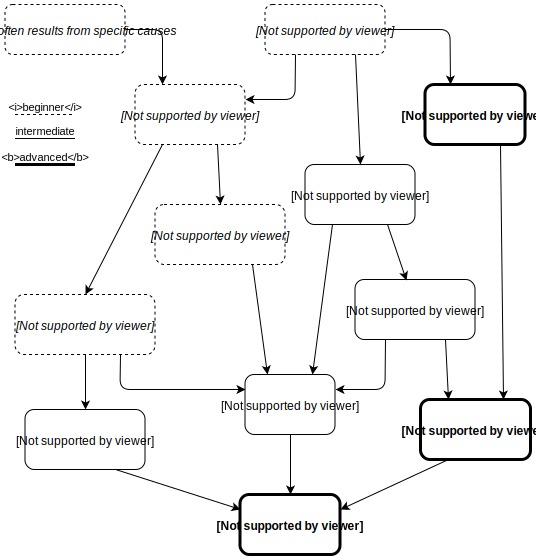
\includegraphics{../../files/conditionals.pdf}

Learning Trajectory for Conditions (from {[}Rich2017{]})

But there can be a world of difference between what instructors teach
and what learners learn, and study after study has shown that teaching
evaluations don't correlate with actual learning outcomes
{[}\protect[\hyperlink{b:Star2014}{Star2014}],\protect[\hyperlink{b:Uttl2017}{Uttl2017}]{]}. To find out how much novices are actually
learning, we therefore have to use other measures or do direct studies.
Taking the former approach, roughly two-thirds of post-secondary
students pass their first computing course, with some variations
depending on class size and so on, but with no significant differences
over time or based on language {[}\protect[\hyperlink{b:Benn2007a}{Benn2007a}],\protect[\hyperlink{b:Wats2014}{Wats2014}]{]}.

How does prior experience affect these results? To find out,
{[}\protect[\hyperlink{b:Wilc2018}{Wilc2018}]{]} compared the performance and confidence of novices
with and without prior programming experience in CS1 and CS2. They found
that novices with prior experience outscored novices without by 10\% in
CS1, but those differences disappeared by the end of CS2. They also
found that women with prior exposure outperformed their male peers in
all areas, but were consistently less confident in their abilities; we
will return to this issue in \protect\hyperlink{SECTION}{s:motivation-inclusivity}.

As for direct studies of how much novices learn, {[}\protect[\hyperlink{b:McCr2001}{McCr2001}]{]}
presented a multi-site international study, which was later replicated
by {[}\protect[\hyperlink{b:Utti2013}{Utti2013}]{]}. According to the first study, ``\ldots{}the
disappointing results suggest that many students do not know how to
program at the conclusion of their introductory courses.'' More
specifically, ``For a combined sample of 216 students from four
universities, the average score was 22.89 out of 110 points on the
general evaluation criteria developed for this study.'' This result may
say as much about teachers' expectations as it does about student
ability, but either way, our fourth recommendation is to \emph{measure and
track results} in ways that can be compared over time, so that you can
tell if your lessons are becoming more or less effective.

\section{Do Languages Matter?}\label{s:pck-language}

The short answer is ``yes'': novices learn to program faster and also
learn more using blocks-based tools like Scratch
(\protect\hyperlink{FIGURE}{f:pck-scratch}) that make syntax errors impossible
{[}\protect[\hyperlink{b:Wein2017b}{Wein2017b}]{]}. And block interfaces encourage exploration in a way
that text does not; like all good tools, Scratch can be learned
accidentally {[}\protect[\hyperlink{b:Malo2010}{Malo2010}]{]}.

Our fifth recommendation is therefore to \emph{start children and teens
with blocks-based interfaces} before moving to text-based systems. The
age qualification is there because Scratch (deliberately) looks like
it's meant for younger users; while imitators like \href{https://developers.google.com/blockly/}{Blockly}
look more grown-up, it can still be hard to convince adults to take
them seriously.

\includegraphics{../../files/scratch.jpg}

Scratch (from https://opensource.com/article/18/4/designing-game-scratch-open-jam)

Scratch has probably been studied more than any other programming tool,
and we know a great deal about how it is used. As just one example,
{[}\protect[\hyperlink{b:Aiva2016}{Aiva2016}]{]} analyzed over 250,000 Scratch projects and found
(among other things) that about 28\% of projects have some blocks that
are never called or triggered. The authors hypothesize that users may be
using them as a scratchpad to keep bits of code they don't (yet) want to
throw away.

{[}\protect[\hyperlink{b:Grov2017}{Grov2017}],\protect[\hyperlink{b:Mlad2017}{Mlad2017}]{]} studied novices learning about loops in
Scratch, Logo, and Python, and found that misconceptions about loops are
minimized when using a block-based language rather than a text-based
language. What's more, as tasks become more complex (such as using
nested loops) the differences become larger.

{[}\protect[\hyperlink{b:Wein2017a}{Wein2017a}]{]} studied people using a tool that allowed them to
switch between blocks and text for programming. They found that
learners tend to migrate from blocks to text over time, but when
learners shifted from text to blocks, their next action was to add a
new type of command. This may be because browsing available commands
is easier with blocks, or because blocks make syntax errors with
unfamiliar new commands impossible. The authors say, ``While it is
often claimed that blocks-based programming environments offer the
advantage of reducing syntax errors, our findings suggest that blocks
also offer information about what is possible in the space and provide
a low-stakes means of exploring unfamiliar code.'' New tools like
\href{https://www.greenfoot.org/frames/}{Stride} are trying to smooth the transition between blocks
and text even further; when combined with programming notebooks like
\href{http://jupyter.org/}{Jupyter} and \href{http://stenci.la/}{Stencila}, they may eventually
eliminate the distinction altogether.

\begin{quote}\setlength{\parindent}{0pt}
\textbf{Harder Than Necessary}

{[}\protect[\hyperlink{b:Stef2013}{Stef2013}]{]} has shown that the creators of programming language
make those languages harder to learn by not doing basic usability
testing. For example, ``\ldots{}the three most common words for
looping in computer science, \texttt{for}, \texttt{while}, and \texttt{foreach}, were rated
as the three most unintuitive choices by non-programmers.'' More
fundamentally, their work shows that C-style syntax (as used in Java
and Perl) is just as hard for novices to learn as a randomly-designed
syntax, but that the syntax of languages such as Python and Ruby is
significantly easier to learn, and the syntax of their own language,
Quorum, is easier still, because they are testing each new feature
before adding it to the language. ({[}\protect[\hyperlink{b:Stef2017}{Stef2017}]{]} is a useful
brief summary of what we actually know about designing programming
languages and why we believe it's true.)
\end{quote}

\subsection{Object-Oriented and Functional Programming}\label{object-oriented-and-functional-programming}

Objects and classes are power tools for experienced programmers, and
many educators advocate an ``objects first'' approach to teaching
programming (though they sometimes disagree on exactly what that means
{[}\protect[\hyperlink{b:Benn2007b}{Benn2007b}]{]}). {[}\protect[\hyperlink{b:Sorv2014}{Sorv2014}]{]} describes and motivates this
approach, and {[}\protect[\hyperlink{b:Koll2015}{Koll2015}]{]} describes three generations of tools
designed to support novice programming in object-oriented environments.

Introducing objects early has a few special challenges.
{[}\protect[\hyperlink{b:Mill2016b}{Mill2016b}]{]} found that most novices using Python struggled to
understand \texttt{self} (which refers to ``this object''): they omitted it in
method definitions, failed to use it when referencing object attributes,
or both. Object reference errors were also more common than other
errors; the authors speculate that this is partly due to the difference
in syntax between \texttt{obj.method(param)} and \texttt{def\ method(self,\ param)}.
{[}\protect[\hyperlink{b:Rago2017}{Rago2017}]{]} found something similar in high school students, and
that high school teachers often weren't clear on the concept either.

Another approach is exemplified by the \href{http://www.bootstrapworld.org/}{Bootstrap project},
which is based on the \protect\hyperlink{g:functional-programming}{functional
programming} paradigm. This work draws on a
rich tradition going back to languages like Scheme and Lisp, and to
classic textbooks like
{[}\protect[\hyperlink{b:Fell2001}{Fell2001}],\protect[\hyperlink{b:Frie1995}{Frie1995}],\protect[\hyperlink{b:Abel1996}{Abel1996}]{]}. If functional
programming continues to gain ground among professional programmers,
this approach may grow more popular for teaching.

On balance, we recommend that instructors \emph{use procedural languages} to
start with, i.e., that defining classes and using higher-order functions
not be taught until learners understand basic control structures and
data types. How quickly these topics should be introduced depends on the
audience: if learners want to build web applications in JavaScript, for
example, they're going to have to master callbacks much earlier than if
they want to generate reports using C\#.

\subsection{Type Declarations}\label{type-declarations}

Programmers have argued for decades about whether variables' data types
should have to be declared or not. One recent empirical finding is
{[}\protect[\hyperlink{b:Gao2017}{Gao2017}]{]}, which found that about 15\% of bugs in JavaScript
programs could be caught by requiring type declarations, which is either
high or low depending on what answer you wanted in the first place.

However, programming and learning to program are different activities,
and results from the former don't necessarily apply to the latter.
{[}\protect[\hyperlink{b:Endr2014}{Endr2014}]{]} found that requiring novices to declare variable
types does add some complexity to programs, but it pays off fairly
quickly by acting as documentation for a method's use---in particular, by
forestalling questions about what's available and how to use it.

We don't know enough yet to recommend typed or untyped languages for
novices. Now that Python allows optional typing, though, it may be
feasible for researchers to explore whether it can or should be
introduced gradually.

\subsection{Does Variable Naming Style Matter?}\label{does-variable-naming-style-matter}

{[}\protect[\hyperlink{b:Kern1999}{Kern1999}]{]} says, ``Programmers are often encouraged to use long
variable names regardless of context. This is a mistake: clarity is
often achieved through brevity.'' Lots of programmers believe this, but
{[}\protect[\hyperlink{b:Hofm2017}{Hofm2017}]{]} found that using full words in variable names led to
an average of 19\% faster comprehension compared to letters and
abbreviations.

In contrast, {[}\protect[\hyperlink{b:Beni2017}{Beni2017}]{]} found that using single-letter variable
names didn't affect novices' ability to modify code. This may be because
their programs are shorter than professionals', or because some
single-letter variable names have implicit types and meanings: most
programmers assume \texttt{i}, \texttt{j}, and \texttt{n} are integers, and \texttt{s} is a string,
while \texttt{x}, \texttt{y}, and \texttt{z} are either floating-point numbers or integers
more or less equally.

How important is this? {[}\protect[\hyperlink{b:Bink2012}{Bink2012}]{]} reported a series of studies
that found that reading and understanding code is fundamentally
different from reading prose: ``\ldots{}the more formal structure
and syntax of source code allows programmers to assimilate and
comprehend parts of the code quite rapidly independent of style. In
particular\ldots{}beacons and program plans play a large role in
comprehension.'' It also found that experienced developers are relatively
unaffected by identifier style, so our recommendation is just to use
consistent style in all examples.

Since most languages have style guides (e.g., \href{https://www.python.org/dev/peps/pep-0008/}{PEP 8} for
Python) and tools to check that code follows these guidelines, our
full recommendation is to \emph{use tools to ensure that all code examples
adhere to a consistent style}.

\section{Does Better Feedback Help?}\label{s:pck-error}

Incomprehensible error messages are a major source of frustration for
novices (and sometimes for experienced programmers as well). Several
researchers have therefore explored whether better error messages would
help alleviate this. For example, {[}\protect[\hyperlink{b:Beck2016}{Beck2016}]{]} rewrote some of the
Java compiler's messages so that instead of:

\begin{lstlisting}
C:\stj\Hello.java:2: error: cannot find symbol
        public static void main(string[ ] args){
^
1 error
Process terminated ... there were problems.
\end{lstlisting}

learners would see:

\begin{lstlisting}
Looks like a problem on line number 2.
If "string" refers to a datatype, capitalize the 's'!
\end{lstlisting}

Sure enough, novices given these messages made fewer repeated errors and
fewer errors overall.

{[}\protect[\hyperlink{b:Bari2017}{Bari2017}]{]} went further and used eye tracking to show that
despite the grumblings of compiler writers, people really do read error
messages---in fact, they spend 13--25\% of their time doing this. However,
reading error messages turns out to be as difficult as reading source
code, and how difficult it is to read the error messages strongly
predicts task performance. Instructors should therefore \emph{give learners
practice in reading and interpreting error messages}. {[}\protect[\hyperlink{b:Marc2011}{Marc2011}]{]}
has a rubric for responses to error messages that can be useful in
grading such exercises.

\subsection{Does Visualization Help?}\label{does-visualization-help}

The idea of visualizing programs is perennially popular, and tools
like {[}\protect[\hyperlink{b:Guo2013}{Guo2013}]{]} (a web-based tool for visualizing the
execution of Python programs) and \href{http://latentflip.com/loupe/}{Loupe} (which shows how
JavaScript's event loop works) are both useful teaching aids.
However, people learn more from constructing visualizations than they
do from viewing visualizations constructed by others
{[}\protect[\hyperlink{b:Stas1998}{Stas1998}],\protect[\hyperlink{b:Ceti2016}{Ceti2016}]{]}, so does visualization actually
help learning?

To answer this, {[}\protect[\hyperlink{b:Cunn2017}{Cunn2017}]{]} replicated an earlier study of the
kinds of sketching students do when tracing code execution. They found
that not sketching at all correlates with lower success, while tracing
changes to variables' values by writing new values near their names as
they change was the most effective strategy (\protect\hyperlink{FIGURE}{f:pck-sketch}).

One possible confounding effect they checked was time: since sketchers
take significantly more time to solve problems, do they do better just
because they think for longer? The answer is no: there was no
correlation between the time taken and the score achieved. Our
recommendation is therefore to \emph{teach students to trace variables'
values when debugging}.

\begin{quote}\setlength{\parindent}{0pt}
\textbf{Flowcharts}

One often-overlooked finding about visualization is that students
understand flowcharts better than pseudocode \emph{if both are equally well
structured} {[}\protect[\hyperlink{b:Scan1989}{Scan1989}]{]}. Earlier work showing that pseudocode
outperformed flowcharts used structured pseudocode and tangled
flowcharts; when the playing field was levelled, novices did better
with the graphical representation.
\end{quote}

\section{What Else Can We Do to Help?}\label{s:pck-help}

{[}\protect[\hyperlink{b:Viha2014}{Viha2014}]{]} examined the average improvement in pass rates of
various kinds of intervention in programming classes. As they themselves
point out, there are many reasons to take their findings with a grain of
salt: the pre-change teaching practices are rarely stated clearly, the
quality of change is not judged, and only 8.3\% of studies reported
negative findings, so either there is positive reporting bias or the way
we're teaching right now is almost the worst way possible and anything
would be an improvement. And like many other studies discussed in this
chapter, they were only looking at university classes, so their findings
may not generalize to other groups.

With all those caveats in mind, they found ten things instructors can do
to improve outcomes (\protect\hyperlink{FIGURE}{f:pck-interventions}):

\begin{description}
\tightlist
\item[Collaboration:]
Activities that encourage student collaboration either in classrooms
or labs.
\item[Content Change:]
Parts of the teaching material were changed or updated.
\item[Contextualization:]
Course content and activities were aligned towards a specific
context such as games or media.
\item[CS0:]
Creation of a preliminary course to be taken before the introductory
programming course; could be organized only for some (e.g., at-risk)
students.
\item[Game Theme:]
A game-themed component was introduced to the course.
\item[Grading Scheme:]
A change in the grading scheme; the most common change was to
increase the amount of points rewarded from programming activities,
while reducing the weight of the course exam.
\item[Group Work:]
Activities with increased group work commitment such as team-based
learning and cooperative learning.
\item[Media Computation:]
Activities explicitly declaring the use of media computation
(\protect\hyperlink{CHAPTER}{s:motivation}).
\item[Peer Support:]
Support by peers in form of pairs, groups, hired peer mentors or
tutors.
\item[Other Support:]
An umbrella term for all support activities, e.g. increased teacher
hours, additional support channels, etc.
\end{description}

\includegraphics{../../files/interventions.png}

Effectiveness of Interventions

This list highlights the importance of cooperative learning.
{[}\protect[\hyperlink{b:Beck2013}{Beck2013}]{]} looked at this specifically over three academic years
in courses taught by two different instructors, and found significant
benefits overall and for many subgroups: they not only had higher
grades, they left fewer questions blank on the final exam, which
indicates greater self-efficacy and willingness to try to debug things.

As noted earlier, writing code isn't the only way to teach people how
to program. {[}\protect[\hyperlink{b:Shel2017}{Shel2017}]{]} reports that having novices work on
computational creativity exercises improves grades at several
levels. A typical exercise is to identify an everyday object (such as
nail clipper, a paper clip, Scotch tape) and describe the object in
terms of its inputs, outputs and functions. This kind of teaching is
sometimes called ``unplugged''; the \href{https://csunplugged.org/en/}{CS Unplugged} site
has a collection of lessons and exercises for doing this.

\section{Exercises}\label{s:pck-exercises}

\subsection{Checking for Common Errors (individual/20)}\label{checking-for-common-errors-individual20}

This list of common errors is taken from {[}\protect[\hyperlink{b:Sirk2012}{Sirk2012}]{]}. Pick three,
and write an exercise for each to check that learners \emph{aren't} making
that mistake.

\begin{description}
\tightlist
\item[Inverted assignment:]
The student assigns the value of the left-hand variable to the
right-hand side variable, rather than the other way around.
\item[Wrong branch:]
Even though the conditional evaluates to \texttt{False}, the student jumps
to the \texttt{then} clause.
\item[Wrong \texttt{False}:]
As soon as the conditional evaluates to \texttt{False} , the student
returns \texttt{False} from the function.
\item[Executing function instead of defining it:]
The student believes that a function is executed as it is defined.
\item[Unevaluated parameters:]
The student believes the function starts running before the
parameters have been evaluated.
\item[Parameter evaluated in the wrong frame:]
The student creates parameter variables in the caller's frame, not
in the callee's.
\item[Failing to store return value:]
The student does not assign the return value in the caller.
\item[Assignment copies object:]
The student creates a new object rather than copying a reference.
\item[Method call without subject:]
The student tries to call a method from a class without first
creating an instance of the class.
\end{description}

\subsection{Mangled Code (pairs/15)}\label{mangled-code-pairs15}

{[}\protect[\hyperlink{b:Chen2017}{Chen2017}]{]} describes exercises in which students reconstruct
code that has been mangled by removing comments, deleting or replacing
lines of code, moving lines, inserting extra unneeded lines, and so on.
Student performance on these correlates strongly with performance on
assessments in which students write code (i.e., whatever traditional
assignments are measuring, these are measuring as well), but these
questions require less (in-person) work to mark. Take the solution to a
programming exercise you've created in the past, mangle it in two
different ways, and swap with a partner.

\subsection{The Rainfall Problem (pairs/10)}\label{the-rainfall-problem-pairs10}

{[}\protect[\hyperlink{b:Solo1986}{Solo1986}]{]} introduced the Rainfall Problem: write a program that
repeatedly reads in positive integers until it reads the integer 99999.
After seeing 99999, the program should print out the average of the
numbers seen. This problem has been used in many subsequent studies of
programming {[}\protect[\hyperlink{b:Fisl2014}{Fisl2014}],\protect[\hyperlink{b:Simo2013}{Simo2013}],\protect[\hyperlink{b:Sepp2015}{Sepp2015}]{]}.

Solve the Rainfall Problem in the programming language of your choice.
Compare your solutions with those of your partner.

\subsection{Roles of Variables (pairs/15)}\label{roles-of-variables-pairs15}

Take a short program you have written (5--15 lines) and classify each of
its variables using the categories defined in
\protect\hyperlink{SECTION}{s:pck-programming}. Compare your classifications with those
of a partner: where did you agree? When you disagreed, did you
understand each other's view?

\subsection{Choose Your Own Adventures (individual/10)}\label{choose-your-own-adventures-individual10}

Which of the three approaches described in {[}\protect[\hyperlink{b:Sorv2014}{Sorv2014}]{]}
(\protect\hyperlink{SECTION}{s:pck-now}) do you use when teaching? Or is your approach
best described in some other way?

\subsection{What Are You Teaching? (individual/10)}\label{what-are-you-teaching-individual10}

Compare the topics you teach to the list developed in {[}\protect[\hyperlink{b:Luxt2017}{Luxt2017}]{]}
(\protect\hyperlink{SECTION}{s:pck-now}). Which topics do you cover? What extra topics
do you cover that aren't in their list?

\subsection{Beneficial Activities (individual/10)}\label{beneficial-activities-individual10}

Look at the list of interventions developed by {[}\protect[\hyperlink{b:Viha2014}{Viha2014}]{]}
(\protect\hyperlink{SECTION}{s:pck-help}). Which of these things do you already do in
your classes? Which ones could you easily add? Which ones are
irrelevant?

\subsection{Visualizations (individual/10)}\label{visualizations-individual10}

What visualization do you most like to use when teaching? Is it a static
image or an animation? Do you show it to your learners, do they discover
it on their own, or something in between?

\subsection{Misconceptions and Challenges (small groups/15)}\label{misconceptions-and-challenges-small-groups15}

The \href{http://www.pd4cs.org/}{Professional Development for CS Principles Teaching} site
includes \href{http://www.pd4cs.org/mc-index/}{a detailed list of student misconceptions and
exercises}. Working in small groups, choose one
section (such as data structures or functions) and go through their
list. Which of these misconceptions do you remember having when you
were a learner? Which do you still have? Which have you seen in your
learners?

\chapter{Teaching as a Performance Art}\label{s:performance}

As \protect\hyperlink{CHAPTER}{s:pck} explained, every teacher needs content knowledge,
general pedagogical knowledge, and pedagogical content knowledge in
order to be effective. We can elaborate this framework by adding
technology to the mix {[}\protect[\hyperlink{b:Koeh2013}{Koeh2013}]{]}, but that doesn't change the
key point: it isn't enough to know the subject, or how to teach---you have
to know how to teach that particular subject {[}\protect[\hyperlink{b:Maye2004}{Maye2004}]{]}.

This chapter therefore focuses on one key aspect of teaching: giving a
lecture or a live demonstration in front of a class. It isn't the only
way to teach, but it is probably the most common, and the techniques
that will make you better at doing it can be applied elsewhere as well.

\begin{quote}\setlength{\parindent}{0pt}
\textbf{Teaching Tips}

The \href{http://csteachingtips.org/}{CS Teaching Tips} site is collecting PCK for
teaching programming, and I hope that one day we will have catalogs
like {[}\protect[\hyperlink{b:Ojos2015}{Ojos2015}]{]}, teacher training materials like
{[}\protect[\hyperlink{b:Hazz2014}{Hazz2014}],\protect[\hyperlink{b:Guzd2015a}{Guzd2015a}],\protect[\hyperlink{b:Sent2018}{Sent2018}]{]}, or more
personal collections like {[}\protect[\hyperlink{b:Gelm2002}{Gelm2002}]{]} to help us all do it
better.
\end{quote}

\section{Lesson Study}\label{s:performance-jugyokenkyu}

From politicians to researchers and teachers themselves, educational
reformers have designed systems to find and promote people who can teach
well and eliminate those who cannot. But the assumption that some people
are born teachers is wrong; instead, like any other performance art, the
keys to better teaching are practice and collaboration. As
{[}\protect[\hyperlink{b:Gree2014}{Gree2014}]{]} explains, the Japanese approach to this is called
\protect\hyperlink{g:jugyokenkyu}{jugyokenkyu}, which means ``lesson study'':

\begin{quote}\setlength{\parindent}{0pt}
\emph{Jugyokenkyu} is a bucket of practices that Japanese teachers use to
hone their craft, from observing each other at work to discussing the
lesson afterward to studying curriculum materials with colleagues. The
practice is so pervasive in Japanese schools that it
is\ldots{}effectively invisible.

In order to graduate, {[}Japanese{]} education majors not only had to
watch their assigned master teacher work, they had to effectively
replace him, installing themselves in his classroom first as
observers and then, by the third week, as a wobbly\ldots{}approximation
of the teacher himself. It worked like a kind of teaching
relay. Each trainee took a subject, planning five days' worth of
lessons\ldots{} {[}and then{]} each took a day. To pass the baton, you had to
teach a day's lesson in every single subject: the one you planned
and the four you did not\ldots{} and you had to do it right under your
master teacher's nose. Afterward, everyone---the teacher, the
college students, and sometimes even another outside
observer---would sit around a formal table to talk about what they
saw.
\end{quote}

Putting work under a microscope in order to improve it is commonplace
in sports and music. A professional musician, for example, will
dissect half a dozen different recordings of ``Body and Soul'' or
``Smells Like Teen Spirit'' before performing it. She would also expect
to get feedback from fellow musicians during practice and after
performances. Many other professions work this way as well: for
example, the Japanese drew inspiration from \href{https://en.wikipedia.org/wiki/W._Edwards_Deming}{Deming's ideas on
continuous improvement in manufacturing}.

But continuous feedback isn't part of teaching culture in most
English-speaking countries. There, what happens in the classroom stays
in the classroom: teachers don't watch each other's lessons on a
regular basis, so they can't borrow each other's good ideas. The
result is that \emph{every teacher has to invent teaching on their
own}. They may get lesson plans and assignments from colleagues, the
school board or a textbook publisher, or go through a few MOOCs on the
Internet, but each teacher has to figure out for herself how to
combine that content with the theory she learned in education school
to deliver an actual lesson in an actual classroom for actual
students.

Writing up new techniques and giving \protect\hyperlink{g:demonstration-lesson}{demonstration
lessons}, in which one person teaches actual
students while other teachers observe, seem like a way to solve
this. However, {[}\protect[\hyperlink{b:Finc2007}{Finc2007}],\protect[\hyperlink{b:Finc2012}{Finc2012}]{]} found that they
are usually ineffective: of the 99 change stories analyzed, teachers
only searched actively for new practices or materials in three cases,
and only consulted published material in eight cases. Most changes
occurred locally, without input from outside sources, or involved only
personal interaction with other educators.

{[}\protect[\hyperlink{b:Bark2015}{Bark2015}]{]} found something similar:

\begin{quote}\setlength{\parindent}{0pt}
Adoption is not a ``rational action,'' however, but an iterative series
of decisions made in a social context, relying on normative
traditions, social cueing, and emotional or intuitive
processes\ldots{} Faculty are not likely to use educational
research findings as the basis for adoption decisions\ldots{}
Positive student feedback is taken as strong evidence by faculty that
they should continue a practice.
\end{quote}

This phenomenon is sometimes called \protect\hyperlink{g:lateral-knowledge-transfer}{lateral knowledge
transfer}: someone sets out to teach X,
but while watching them, their audience actually learns Y as well (or
instead). For example, a teacher might intend to show learners how to
search for email addresses in a text file, but what her audience might
take away is some new keyboard shortcuts in the editor. What
\emph{jugyokenkyu} does is maximize the opportunity for this to happen
between teachers.

\section{Giving and Getting Feedback on Teaching}\label{s:performance-feedback}

Observing someone helps you; giving them feedback helps them. But as the
cartoon in \protect\hyperlink{FIGURE}{f:performance-feedback-feelings} suggests, it can
be hard to receive feedback, especially when it's negative.

\includegraphics{../../files/deathbulge-jerk.jpg}

Feedback Feelings (copyright © Deathbulge 2013)

Feedback is easier to give and receive when both parties share ground
rules and expectations. This is especially important when they have
different backgrounds or cultural expectations about what's appropriate
to say and what isn't. You can get better feedback on your work by using
these techniques:

\begin{description}
\item[Initiate feedback.]
It's better to ask for feedback than to receive it unwillingly.
\item[Choose your own questions,]
i.e., ask for specific feedback. It's a lot harder for someone to
answer, ``What do you think?'' than to answer either, ``What is one
thing I could have done as a teacher to make this lesson more
effective?'' or ``If you could pick one thing from the lesson to go
over again, what would it be?''

Directing feedback like this is also more helpful to you. It's
always better to try to fix one thing at once than to change
everything and hope it's for the better. Directing feedback at
something you have chosen to work on helps you stay focused, which
in turn increases the odds that you'll see progress.
\item[Use a feedback translator.]
Have someone else read over all the feedback and give you a summary.
It can be easier to hear ``It sounds like most people are following,
so you could speed up'' than to read several notes all saying, ``this
is too slow'' or ``this is boring''.
\item[Be kind to yourself.]
Many of us are very critical of ourselves, so it's always helpful to
jot down what we thought of ourselves \emph{before} getting feedback from
others. That allows us to compare what we think of our performance
with what others think, which in turn allows us to scale the former
more accurately. For example, it's very common for people to think
that they're saying ``um'' and ``err'' all the time, when their audience
doesn't notice it. Getting that feedback once allows teachers to
adjust their assessment of themselves the next time they feel that
way.
\end{description}

You can give feedback to others more effectively as well:

\begin{description}
\tightlist
\item[Balance positive and negative feedback.]
A common method is a ``compliment sandwich'' made up of one positive,
one negative, and a second positive observation (though this can get
tiresome after a while).
\item[Organize your feedback using a rubric.]
Most people are more comfortable giving and receiving feedback when
they feel that they understand the social rules governing what they
are allowed to say and how they are allowed to say it. A facilitator
can then transcribe items into a shared document (or onto a
whiteboard) during discussion.
\end{description}

The simplest rubric for feedback on teaching is a 2x2 grid whose
vertical axis is labelled ``what went well'' and ``what can be improved'',
and whose horizontal axis is labelled ``content'' (what was said) and
``presentation'' (how it was said). Observers write their comments on
sticky notes as they watch the demonstration, then post those in the
quadrants of a grid drawn on a whiteboard
(\protect\hyperlink{FIGURE}{f:performance-rubric}).


\includegraphics{../../files/2x2-rubric.pdf}

Teaching Rubric

A more sophisticated rubric developed for assessing 5--10 minute videos
of programming instruction is given in \protect\hyperlink{APPENDIX}{s:teacheval}. A
rubric this detailed is best presented as a checklist with items more or
less in the order that they'll be used (e.g., questions about the
introduction come before questions about the conclusion).

\begin{quote}\setlength{\parindent}{0pt}
\textbf{Question Budgets}

Rubrics like the one in \protect\hyperlink{APPENDIX}{s:teacheval} have a tendency to
grow over time as people think of things they'd like to add. A good
way to keep them manageable is to insist that the total length stay
constant, i.e., that if someone wants to add a question, they have to
identify one that's less important and can be removed.
\end{quote}

If you are interested in giving and getting feedback, {[}\protect[\hyperlink{b:Gorm2014}{Gorm2014}]{]}
has good advice that you can use to make peer-to-peer feedback a routine
part of your teaching, while {[}\protect[\hyperlink{b:Gawa2011}{Gawa2011}]{]} looks at the value of
having a coach. However feedback is collected, remember that it is meant
to be formative: its goal is to help people figure out what they are
doing well and what they still need to work on. Please also remember
that these guidelines are for peer-to-peer feedback on your lesson
delivery; gathering feedback from your learners should be as close to
continuous as you can make it, and you should prompt for questions and
reflections as well as positives and negatives.

\begin{quote}\setlength{\parindent}{0pt}
\textbf{Studio Classes}

Architecture schools often include studio classes, in which students
solve small design problems and get feedback from their peers right
then and there. These classes are most effective when the teacher
critiques both the designs and the peer critiques, so that
participants learn not only how to make buildings, but how to give and
get feedback {[}\protect[\hyperlink{b:Scho1984}{Scho1984}]{]}. Master classes in music serve a
similar purpose.
\end{quote}

\section{How to Practice Performance}\label{s:performance-practice}

The best way to improve your in-person lesson delivery is to watch
yourself do it. This method is borrowed from Warren Code at the
University of British Columbia.

\begin{enumerate}
\item
  Work in groups of three.
\item
  Each person rotates through the roles of teacher, audience, and
  videographer. The teacher has two minutes to explain one key idea
  from their teaching or other work as if they were talking to a class
  of high school students. The person pretending to be the audience is
  there to be attentive, while the videographer records the session
  using a cellphone or other handheld device.
\item
  After everyone has finished teaching, the whole group watches the
  videos together. Everyone gives feedback on all three videos, i.e.,
  people give feedback on themselves as well as on others.
\item
  After the videos have been discussed, they are deleted. (Many people
  are increasingly uncomfortable with the prospect of images of
  themselves appearing online.)
\item
  Finally, return to the main group and add the feedback to a shared
  2x2 grid that separates positive from negative and content from
  presentation.
\end{enumerate}

In order for this exercise to work well:

\begin{itemize}
\item
  Record all three videos and then watch all three. If the cycle is
  teach-review-teach-review, the last person to teach runs out of
  time. Doing all the reviewing after all the teaching also helps put
  a bit of distance between the teaching and the reviewing, which
  makes the exercise slightly less excruciating.
\item
  Let people know at the start of the class that they will be asked to
  teach something so that they have time to choose a topic. (Telling
  them this in advance can be counter-productive, since some people
  will fret over how much they should prepare.)
\item
  Groups must be physically separated to reduce audio cross-talk
  between their recordings. In practice, this means 2--3 groups in a
  normal-sized classroom, with the rest using nearby breakout spaces,
  coffee lounges, offices, or (on one occasion) a janitor's storage
  closet.
\item
  People must give feedback on themselves, as well as giving feedback
  on each other, so that they can calibrate their impressions of their
  own teaching according to the impressions of other people. (Most
  people are harder on themselves than others are, and it's important
  for them to realize this.)
\end{itemize}

The announcement of this exercise is often greeted with groans and
apprehension, since few people enjoy seeing or hearing themselves.
However, those same people consistently rate it as one of the most
valuable parts of workshops based on these notes. It's also good
preparation for co-teaching (\protect\hyperlink{SECTION}{s:classroom-together}):
teachers find it a lot easier to give each other informal feedback if
they have had some practice doing so and have a shared rubric to set
expectations.

\begin{quote}\setlength{\parindent}{0pt}
\textbf{Tells}

Everyone has nervous habits. For example, many of us talk more rapidly
and in a higher-pitched voice than usual, while others play with their
hair or crack their knuckles. Gamblers call nervous habits like this
``tells''. While these are often not as noticeable as you would think,
it's good to know whether you pace, fiddle with your hair, look at
your shoes, or rattle the change in your pocket when you don't know
the answer to a question.

You can't get rid of tells completely, and trying to do so can make
you obsess about them. A better strategy is to try to displace them,
e.g., to train yourself to scrunch your toes inside your shoes instead
of cracking your knuckles.
\end{quote}

\section{Live Coding}\label{s:performance-live}

\begin{quote}\setlength{\parindent}{0pt}
Teaching is theater, not cinema.

--- Neal Davis
\end{quote}

One technique that completely changed the way I teach programming is
\protect\hyperlink{g:live-coding}{live coding}. Instead of using slides,
teachers actually write code in front of their class as their learners
follow along. It's more effective than slides for many reasons:

\begin{itemize}
\item
  Watching a program being written is more compelling than watching
  someone page through slides that present bits and pieces of the same
  code.
\item
  It enables teachers to be more responsive to ``what if?'' questions.
  Where a slide deck is like a railway track, live coding allows
  teachers to go off road and follow their learners' interests.
\item
  It facilitates lateral knowledge transfer: people learn more than we
  realized we were teaching by watching \emph{how} teachers do things.
\item
  It slows the teacher down: if she has to type in the program as she
  goes along, she can only go twice as fast as her learners, rather
  than ten-fold faster as she could with slides.
\item
  It helps to keep the load on short-term memory down because it makes
  the teacher more aware of how much they are throwing at their
  learners. (This isn't true of slides or of copy-and-paste.)
\item
  Learners get to see teachers' mistakes \emph{and how to diagnose and
  correct them}. Novices are going to spend most of their time doing
  this, but it's left out of most textbooks.
\item
  Watching teachers make mistakes shows learners that it's all right
  to make mistakes of their own. Most people model the behavior of
  their teachers: if the teacher isn't embarrassed about making and
  talking about mistakes, learners will be more comfortable doing so
  too.
\end{itemize}

Teachers need a bit of practice to get comfortable with thinking aloud
as they code in front of an audience, but most report that it is then no
more difficult than talking around a deck of slides, and research seems
to back up its effectiveness {[}\protect[\hyperlink{b:Rubi2013}{Rubi2013}],\protect[\hyperlink{b:Haar2017}{Haar2017}]{]}. The sections
below offer tips on how to make your live coding better.

\subsection{Embrace Your Mistakes}\label{embrace-your-mistakes}

\begin{quote}\setlength{\parindent}{0pt}
The typos are the pedagogy.

--- Emily Jane McTavish
\end{quote}

The most important rule of live coding is to embrace your mistakes. No
matter how well you prepare, you will make some; when you do, think
through them with your audience. While data is hard to come by,
professional programmers spend anywhere from 25\% to 60\% of their time
debugging; novices spend much more (\protect\hyperlink{SECTION}{s:pck-debug}), but most
textbooks and tutorials spend little time diagnosing and correct
problems. If you talk aloud while you figure out what you mistyped or
where you took the wrong path, and explain how you've corrected
yourself, you will give your learners a toolbox they can use when they
make their own mistakes.

This is at odds with advice like that in {[}\protect[\hyperlink{b:Kran2015}{Kran2015}]{]}, which
says, ``\ldots{}you should have your material \emph{absolutely mastered} before
you enter the classroom. If\ldots{}you have a proof or example that is not
quite right\ldots{}and stand in front of the group trying to fix it, then
you will lose all but the diehards quickly.'' In contrast, the feedback
we've had in \href{http://software-carpentry.org}{Software Carpentry} workshops and other settings is
that watching the teacher make mistakes actually motivates most
students, since it gives them permission to be less than perfect as
well.

\begin{quote}\setlength{\parindent}{0pt}
\textbf{Deliberate Fumbles}

If you've given a lesson several times, you're unlikely to make
anything other than basic typing mistakes (which can still be
informative). You can try to remember past mistakes and make them
deliberately, but that often feels forced (unless the mistake and
how to correct it is the primary purpose of the lesson). A better
approach is sometimes called \protect\hyperlink{g:twitch-coding}{twitch coding}: ask
learners one by one to tell you what to type next. This is pretty
much guaranteed to get you into the weeds.
\end{quote}

\subsection{Ask For Predictions}\label{ask-for-predictions}

One way to keep students engaged while you are live coding is to ask
them to make predictions, e.g., to say, ``What is going to happen when I
run this code?'' You can then either show them, or write down the first
few suggestions they make, have the whole class vote on which they think
is most likely, and then run the code. As well as keeping their
attention on task, this gives them practice at reasoning about code's
behavior, which is a useful skill in its own right.

\subsection{Take It Slow}\label{take-it-slow}

For every command you type, every word of code you write, every menu
item or website button you click, say out loud what you are doing while
you do it, then point to the command and its output on the screen and go
through it a second time. This not only slows you down, it allows
learners who are following along to copy what you do, or to catch up,
even when they are looking at their screen while doing it. Whatever you
do, \emph{don't} copy and paste code: doing this practically guarantees that
you'll race ahead of your learners. And if you use tab completion, say
it out loud the first few times so that your learners understand what
you're doing: ``Let's use turtle dot `r' `i' and tab to get `right'.''

If the output of your command or code makes what you just typed
disappear from view, scroll back up so learners can see it again. If
that's not practical, execute the same command a second time, or copy
and paste the last command(s) into the workshop's shared notes.

\subsection{Be Seen and Heard}\label{be-seen-and-heard}

If you are physically able to stand up for a couple of hours, do it
while you are teaching. When you sit down, you are hiding yourself
behind others for those sitting in the back rows. Make sure to notify
the workshop organizers of your wish to stand up and ask them to arrange
a high table, standing desk, or lectern.

Regardless of whether you are standing or sitting, make sure to move
around as much as reasonable. You can for example go to the screen to
point something out, or draw something on the white/blackboard (see
below). Moving around makes the teaching more lively, less monotonous.
It draws the learners' attention away from their screens, to you, which
helps get the point you are making across.

Even though you may have a good voice and know how to use it well, it
may be a good idea to use a microphone, especially if the workshop room
is equipped with one. Your voice will be less tired, and you increase
the chance of people with hearing difficulties being able to follow the
workshop.

\subsection{Mirror Your Learner's Environment}\label{mirror-your-learners-environment}

You may have customized your environment with a fancy Unix shell prompt,
a custom color scheme for your development environment, or a plethora of
keyboard shortcuts. Your learners won't have any of this, so try to
create an environment that mirrors what they \emph{do} have. Some teachers
create a separate bare-bones user (login) account on their laptop, or a
separate teaching-only account if they're using an online service like
Scratch or GitHub.

\subsection{Use the Screen Wisely}\label{use-the-screen-wisely}

You will need to enlarge your font considerably in order for people to
read it from the back of the room, which means you can put much less on
the screen than you're used to. You will often be reduced to 60--70
columns and 20--30 rows, which basically means that you're using a 21st
Century supercomputer to emulate an early-1980s VT100 terminal.

To cope with this, maximize your window, and then ask everyone to give
you a thumbs-up or thumbs-down on its readability. Use a black font on a
lightly-tinted background rather than a light font on a dark
background---the light tint will glare less than a pure white
background.

Pay attention to the room lighting as well: it should not be fully dark,
and there should be no lights directly on or above the presenter's
screen. If needed, reposition the tables so all learners can see the
screen.

When the bottom of the projector screen is at the same height, or below,
the heads of the learners, people in the back won't be able to see the
lower parts. Raise the bottom of your window(s) to compensate, but be
aware that this gives you even less space for your typing.

If you can get a second projector and screen, use it: the extra real
estate will allow you to display your code on one side and its output or
behavior on the other. The second screen may require its own PC or
laptop, so you may need to ask a helper to control it.

If you teach using a console window, such as a Unix shell, it's
important to tell people when you run an in-console text editor and when
you return to the console prompt. Most novices have never seen a window
take on multiple personalities in this way, and can quickly become
confused (particularly if the window is hosting an interactive
interpreter prompt for Python or some other language as well as running
shell commands and hosting an editor).

\begin{quote}\setlength{\parindent}{0pt}
\textbf{Accessibility Aids Help Everyone}

Tools like \href{https://boinx.com/mousepose/overview/}{Mouseposé} (for Mac) and
\href{http://www.pointerfocus.com/}{PointerFocus} (for Windows) will highlight the
position of your mouse cursor on the screen, and screen recording
software tools like \href{https://www.techsmith.com/video-editor.html}{Camtasia} will echo invisible keys
like tab and Control-J as you type them. These take a bit of
practice to get used to, but are extremely helpful as you start
teaching more advanced tools.
\end{quote}

\subsection{Double Devices}\label{double-devices}

Some people now use two devices when teaching: a laptop plugged into the
projector for learners to see, and a tablet beside it so that they can
view their own notes and the shared notes that the learners are taking
together (\protect\hyperlink{SECTION}{s:classroom-notetaking}). This is more reliable
than displaying one virtual desktop while flipping back and forth to
another. Of course, printouts of the lesson material are still the most
reliable backup technology\ldots{}

\subsection{Use Diagrams}\label{use-diagrams}

Diagrams are almost always a good idea. Creating them in advance to
bring up on screen is a common practice---I often have a slide deck full
of diagrams in the background when I'm doing live coding---but don't
underestimate the value of sketching on the whiteboard as you go through
your lesson. This allows you to build diagrams step by step, which helps
with retention (\protect\hyperlink{SECTION}{s:load-split-attention}) and allows you to
improvise.

\subsection{Avoid Distractions}\label{avoid-distractions}

Turn off any notifications you may use on your laptop, such as those
from social media, email, etc. Seeing notifications flash by on the
screen distracts you as well as the learners, and it can be awkward when
a message pops up you'd rather not have others see. If you are teaching
frequently, you might want to create a second account on your computer
that doesn't have email or other tools set up at all.

\subsection{Improvise After You Know the Material}\label{improvise-after-you-know-the-material}

The first time you teach a new lesson, stick fairly closely to the
lesson plan you've drawn up or borrowed. It may be tempting to deviate
from the material because you would like to show a neat trick or
demonstrate some alternative way of doing something. Resist: there is a
fair chance you'll run into something unexpected that you then have to
explain.

Once you are more familiar with the material, though, you can and should
start improvising based on the backgrounds of your learners, their
questions in class, and what you find most interesting about the lesson.
This is like playing a new song: the first few times, you stick to the
sheet music, but after you're comfortable with it, you can start to put
your own stamp on it.

If you really want to use something outside of the material, run through
it beforehand as you plan to in class \emph{using the same computer that
you'll be teaching on}. Installing several hundred megabytes of
software updates over high school WiFi in front of increasingly bored
16-year-olds isn't something you want to do twice.

\begin{quote}\setlength{\parindent}{0pt}
\textbf{Direct Instruction}

\protect\hyperlink{g:direct-instruction}{Direct Instruction} is a teaching
method centered around meticulous curriculum design delivered through
a prescribed script---i.e., it's more like an actor reciting lines than
it is like the improvisatory approach we recommend. {[}\protect[\hyperlink{b:Stoc2018}{Stoc2018}]{]}
surveys studies and finds statistically significant positive effect,
even though DI sometimes gets knocked for being mechanical. We still
prefer improvisation because DI requires a far greater up-front
investment than most free-range learning groups can afford.
\end{quote}

\subsection{Face the Screen---Occasionally}\label{face-the-screenoccasionally}

It's OK to face the screen occasionally, particularly when you are
walking through a section of code statement by statement or drawing a
diagram, but you shouldn't do this for more than a few seconds at a
time. Looking at the screen for a few seconds can help lower your
anxiety levels, since it gives you a brief break from being looked at.

A good rule of thumb is to treat the screen as one of your learners: if
it would be uncomfortable to stare at someone for as long as you are
spending looking at the screen, it's time to turn around and face your
audience.

\subsection{Drawbacks}\label{drawbacks}

Live coding does have some drawbacks, but with practice, these can be
avoided or worked around. A common one is going too slowly, either
because you are not a good typist or because you are spending too much
time looking at notes trying to figure out what to type next. The fix
for the first is a bit of typing practice; the fix for the second is to
break the lesson into very short pieces, so that you only ever have to
remember one small step to take next.

A deeper exercise is that typing in library import statements, class
headers, and other boilerplate code increases the extraneous cognitive
load on your learners (\protect\hyperlink{CHAPTER}{s:load}). If you spend a lot of time
doing this, it may be all that learners take away, so give yourself and
your learners skeleton code to start with
(\protect\hyperlink{SECTION}{s:classroom-blank}).

\section{Exercises}\label{s:performance-exercises}

\subsection{Give Feedback on Bad Teaching (whole class/20)}\label{give-feedback-on-bad-teaching-whole-class20}

\begin{enumerate}
\item
  Watch \href{https://www.youtube.com/watch?v=-ApVt04rB4U}{this video of bad teaching} as a group
  and give feedback on it. Organize feedback along two axes: positive
  vs. negative and content vs. presentation.
\item
  Have each person in the class add one point to a 2x2 grid on a
  whiteboard (or in the shared notes) without duplicating any points
  that are already up there.
\end{enumerate}

What did other people see that you missed? What did they think that you
strongly agree or disagree with?

\subsection{Practice Giving Feedback (small groups/45)}\label{practice-giving-feedback-small-groups45}

Use the process described above to practice teaching in groups of
three. When your group is done, the teacher will add one point of
feedback from each participant to a 2x2 grid on the whiteboard or in
the shared notes, without accepting duplicates. Participants should
not say whether the point they offer was made by them, about them, or
neither: the goal at this stage is primarily for people to become
comfortable with giving and receiving feedback, and to establish a
consensus about what sorts of things to look for.

\subsection{The Bad and the Good (whole class/20)}\label{the-bad-and-the-good-whole-class20}

Watch the videos of \href{https://youtu.be/bXxBeNkKmJE}{live coding done poorly}
and \href{https://youtu.be/SkPmwe_WjeY}{live coding done well} and summarize your
feedback on both using the usual 2x2 grid. These videos assume
learners know what a shell variable is, know how to use the \texttt{head}
command, and are familiar with the contents of the data files being
filtered.

\subsection{See Then Do (pairs/30)}\label{see-then-do-pairs30}

Teach 3--4 minutes of a lesson using live coding to a fellow trainee,
then swap and watch while that person live codes for you. Don't bother
trying to record the live coding sessions---we have found that it's
difficult to capture both the person and the screen with a handheld
device---but give feedback the same way you have previously (positive and
negative, content and presentation). Explain in advance to your fellow
trainee what you will be teaching and what the learners you teach it to
are expected to be familiar with.

\begin{itemize}
\item
  What felt different about live coding (versus standing up and
  lecturing)? What was harder/easier?
\item
  Did you make any mistakes? If so, how did you handle them?
\item
  Did you talk and type at the same time, or alternate?
\item
  How often did you point at the screen? How often did you highlight
  with the mouse?
\item
  What will you try to do differently next time?
\end{itemize}

\subsection{Tells (small groups/15)}\label{tells-small-groups15}

\begin{enumerate}
\item
  Read the description of tells at the end of
  \protect\hyperlink{SECTION}{s:performance-feedback}, then make a note of what you
  think your tells are, but do not share them with other people.
\item
  Teach a short (3--5 minute) lesson.
\item
  Ask your audience how they think you betray nervousness. Is their
  list the same as yours?
\end{enumerate}

\subsection{Teaching Tips (small groups/15)}\label{teaching-tips-small-groups15}

The \href{http://csteachingtips.org/}{CS Teaching Tips} site has a large number of
practical tips on teaching computing, as well as a collection of
downloadable tip sheets. In small groups, go through the tip sheets on
their home page and classify each tip as ``use all the time'', ``use
occasionally'', ``never use''. Where do your practice and your peers'
practice differ? Are there any tips you strongly disagree with, or
think would be ineffective?

\chapter{In the Classroom}\label{s:classroom}

The previous chapter described how to practice in-class teaching and
described one method---live coding---that allows teachers to adapt to their
learners' pace and interests. This chapter describes other practices
that have proven helpful in programming classes.

Before describing these practices, it's worth pausing for a moment to
set expectations. The best teaching method we know is individual
tutoring: {[}\protect[\hyperlink{b:Bloo1984}{Bloo1984}]{]} found that students taught one-to-one using
mastery learning techniques performed two standard deviations better
than those who learned through conventional lecture, i.e., that
individually-tutored students did better than 98\% of students who were
lectured to. However, hiring one teacher for every student is impossibly
expensive (and despite the hype, artificial intelligence isn't going to
take the place of human instructors any time soon). Every method is
essentially an attempt to get as much of the value of individual
attention as possible, but at scale.

\section{Enforce the Code of Conduct}\label{s:classroom-enforce}

\protect\hyperlink{CHAPTER}{s:intro} said that every workshop should have and enforce a
Code of Conduct like the one in \protect\hyperlink{APPENDIX}{s:conduct}. If you are a
teacher, and believe that someone has violated it, you may warn them,
ask them to apologize, and/or expel them, depending on the severity of
the violation and whether or not you believe it was intentional.
Whatever you do:

\begin{description}
\tightlist
\item[Do it in front of witnesses.]
Most people will tone down their language and hostility in front of
an audience, and having someone else present ensures that later
discussion doesn't degenerate into conflicting claims about who said
what.
\item[If you expel someone, say so to the rest of the class and explain why.]
This helps prevent exaggerated rumors from taking hold, and
also signals very clearly to everyone that you're serious about
making your class safe and respectful for them.
\item[Contact the host of your class]
as soon as you can and describe what happened.
\end{description}

A Code of Conduct is meaningless without procedures for reporting
violations and enforcing its rules. However much you don't enjoy doing
the latter, remember that the former can be a much greater burden for
people who have been targets.

\section{Peer Instruction}\label{s:classroom-peer}

No matter how good a teacher is, she can only say one thing at a time.
How then can she clear up many different misconceptions in a reasonable
time? The best solution developed so far is a technique called
\protect\hyperlink{g:peer-instruction}{peer instruction}. Originally created
by Eric Mazur at Harvard {[}\protect[\hyperlink{b:Mazu1996}{Mazu1996}]{]}, it has been studied
extensively in a wide variety of contexts, including programming
{[}\protect[\hyperlink{b:Crou2001}{Crou2001}],\protect[\hyperlink{b:Port2013}{Port2013}]{]}, and {[}\protect[\hyperlink{b:Port2016}{Port2016}]{]} found that students
value peer instruction even at first contact.

Peer instruction is essentially a way to provide one-to-one mentorship
in a scalable way. It interleaves formative assessment with student
discussion as follows:

\begin{enumerate}
\item
  Give a brief introduction to the topic.
\item
  Give students a multiple choice question that probes for
  misconceptions (rather than simple factual knowledge).
\item
  Have all the students vote on their answers to the MCQ.

  \begin{itemize}
  \item
    If the students all have the right answer, move on.
  \item
    If they all have the same wrong answer, address that specific
    misconception.
  \item
    If they have a mix of right and wrong answers, give them several
    minutes to discuss those answers with one another in small
    groups (typically 2--4 students) and then reconvene and vote
    again.
  \end{itemize}
\end{enumerate}

As \href{https://www.youtube.com/watch?v=2LbuoxAy56o}{this video from Avanti's learning center in
Kanpur} shows, group discussion significantly
improves students' understanding because it forces them to clarify
their thinking, which can be enough to call out gaps in
reasoning. Re-polling the class then lets the teacher know if they can
move on, or if further explanation is necessary. A final round of
additional explanation and discussion after the correct answer is
presented gives students one more chance to solidify their
understanding.

But could this be a false positive? Are results improving because of
increased understanding during discussion, or simply from a
follow-the-leader effect (``vote like Jane, she's always right'')?
{[}\protect[\hyperlink{b:Smit2009}{Smit2009}]{]} tested this by following the first question with a
second one that students answer individually. Sure enough, peer
discussion actually does enhance understanding, even when none of the
students in a discussion group originally knew the correct answer.

\begin{quote}\setlength{\parindent}{0pt}
\textbf{Taking a Stand}

It is important to have learners vote publicly so that they can't
change their minds afterward and rationalize it by making excuses to
themselves like ``I just misread the question''. Much of the value of
peer instruction comes from the hypercorrection of having their answer
be wrong and having to think through the reasons why
(\protect\hyperlink{SECTION}{s:individual-strategies}).
\end{quote}

\section{Teach Together}\label{s:classroom-together}

\protect\hyperlink{g:co-teaching}{Co-teaching} describes any situation in
which two teachers work together in the same classroom.
{[}\protect[\hyperlink{b:Frie2016}{Frie2016}]{]} describes several ways to do this:

\begin{description}
\tightlist
\item[Team teaching:]
Both teachers deliver a single stream of content in tandem, taking
turns the way that musicians taking solos would.
\item[Teach and assist:]
Teacher A teaches while Teacher B moves around the classroom to help
struggling students.
\item[Alternative teaching:]
Teacher A provides a small set of students with more intensive or
specialized instruction while Teacher B delivers a general lesson to
the main group.
\item[Teach and observe:]
Teacher A teaches while Teacher B observes the students, collecting
data on their understanding to help plan future lessons.
\item[Parallel teaching:]
The class is divided into two equal groups and the teachers present
the same material simultaneously to each.
\item[Station teaching:]
The students are divided into several small groups that rotate from
one station or activity to the next while both teachers supervise
where needed.
\end{description}

All of these models create more opportunities for lateral knowledge
transfer than teaching alone. Team teaching is particularly beneficial
in day-long workshops: not only does it give each teacher's voice a
chance to rest, it reduces the risk that they will be so tired by the
end of the day that they will start snapping at their students or
fumbling at their keyboard.

\begin{quote}\setlength{\parindent}{0pt}
\textbf{Helping}

Many people who aren't comfortable teaching are still willing and able
to provide in-class technical support. They can help learners with
setup and installation, answer technical questions during exercises,
monitor the room to spot people who may need help, or keep an eye on
the shared notes (\protect\hyperlink{SECTION}{s:classroom-notetaking}) and either
answer questions there or remind the instructor to do so during
breaks.

Helpers are sometimes people training to become teachers (i.e.,
they're Teacher B in the teach and assist model), but they can also
be members of the host institution's technical support staff, alumni,
or advanced learners who already know the material well. Using the
latter as helpers is doubly effective: not only are they more likely
to understand the problems their peers are having, it also stops them
from getting bored.
\end{quote}

If you and a partner are co-teaching, try to follow these rules:

\begin{itemize}
\item
  Take 2--3 minutes before the start of each class to confirm who's
  teaching what with your partner. (If you have time to do some
  advance preparation, try drawing a concept map together.)
\item
  Use that time to work out a couple of hand signals as well. ``You're
  going too fast'', ``speak up'', ``that learner needs help'', and, ``It's
  time for a bathroom break'' are all useful.
\item
  Each person should teach for at least 10--15 minutes at a stretch,
  since students may be distracted by more frequent interleaving.
\item
  The person who \emph{isn't} teaching shouldn't interrupt, offer
  corrections, elaborations, or amusing personal anecdotes, or do
  anything else to distract from what the person teaching at the time
  is doing or saying. The one exception is that it's sometimes helpful
  to ask leading questions, particularly if the learners seem unsure
  of themselves.
\item
  Each person should take a couple of minutes before they start
  teaching to see what their partner is going to teach after they're
  done, and then \emph{not} present any of that material.
\item
  The person who isn't teaching should stay engaged with the class,
  not catch up on their email. Monitor the shared notes
  (\protect\hyperlink{SECTION}{s:classroom-notetaking}), keep an eye on the students
  to see who's struggling, jot down some feedback to give your
  teaching partner at the next break---anything that contributes to the
  lesson is better than anything that doesn't.
\end{itemize}

Most importantly, take a few minutes when the class is over to either
congratulate or commiserate with each other. In teaching as in life,
shared misery is lessened and shared joy increased: no one will
understand how pleased you are that you helped someone understand loops
better than the person you just taught with.

\section{Assess Prior Knowledge}\label{s:classroom-prior}

The more you know about your learners before you start teaching, the
more you will be able to help them. If you're working inside a formal
school system, you can probably infer their incoming knowledge by
looking at what's (actually) covered in the prerequisites to your
course. If you're in a free-range setting, though, your learners may be
much more diverse, so you may want to give them a short survey or
questionnaire in advance of your class to find out what they do and
don't already know.

But doing this is risky. School trains people to treat all assessment as
summative, i.e., to believe that anything that looks like an exam is
something they have to pass, rather than a chance to shape instruction.
If they answer ``I don't know'' to even a handful of questions on your
preassessment, they might conclude that your class is too advanced for
them. In short, you might scare off many of the people you most want to
help.

And self-assessment is unreliable because of the \href{https://en.wikipedia.org/wiki/Dunning\%E2\%80\%93Kruger_effect}{Dunning-Kruger
effect} {[}\protect[\hyperlink{b:Krug1999}{Krug1999}]{]}: the less people know
about a subject, the less accurate their estimate of their knowledge
is. Conversely, people who are competent may underrate their skills
because they regard their level of competence as normal.

Rather than asking people to rate their knowledge from 1 to 5, you
should therefore try to ask them how easily they could complete some
specific tasks, but that still runs the risk of scaring them away.
\protect\hyperlink{APPENDIX}{s:preassess} presents a short preassessment questionnaire
that most potential learners are unlikely to find intimidating; if you
use it or anything like it, please be sure to follow up with people who
\emph{don't} respond to find out why not.

\section{Plan for Mixed Abilities}\label{s:classroom-mixed}

If your learners have widely varying levels of prior knowledge, then you
can easily wind up in a situation where a third of your class is lost
and a third is bored. That's unsatisfying for everyone, but there are
some strategies you can use to manage the situation:

\begin{itemize}
\item
  Before running a workshop, communicate its level clearly to everyone
  who's thinking of signing up by listing the topics that will be
  covered and showing a few examples of exercises that they will be
  asked to complete.
\item
  Provide extra self-paced exercises so that more advanced learners
  don't finish early and get bored.
\item
  Ask more advanced learners to help people next to them. They'll
  learn from answering their peers' questions (since it will force
  them to think about things in new ways).
\item
  Keep an eye out for learners who are falling behind and intervene
  early so that they don't become frustrated and give up.
\end{itemize}

The most important thing is to accept that no single lesson can possibly
meet everyone's individual needs. If you slow down to accommodate two
people who are struggling, the other 38 are not being well served.
Equally, if you spend a few minutes talking about an advanced topic to a
learner who is bored, the rest of the class will feel left out.

\begin{quote}\setlength{\parindent}{0pt}
\textbf{False Beginners}

A \protect\hyperlink{g:false-beginner}{false beginner} is someone who has
studied a language before but is learning it again. False beginners
may be indistinguishable from
\protect\hyperlink{g:absolute-beginner}{absolute beginners} on preassessment
tests, but are able to move much more quickly through the material
once they start---in mathematical terms, their intercept is the same,
but their slope is very different. False beginners are common in
free-range programming classes: for example, a child may have taken a
Scratch class a couple of years ago and built a mental model of loops
and conditionals, but do poorly on a pre-test because the material
isn't fresh in their mind. All of the strategies described above can
be used in classes with false beginners.

Being a false beginner is an example of
\protect\hyperlink{g:preparatory-privilege}{preparatory privilege}
{[}\protect[\hyperlink{b:Marg2010}{Marg2010}]{]}. In many cases, it's a result of coming from a home
that's secure enough and affluent enough to have several computers and
parents who are familiar with how to use them. Whether or not this is
fair depends on what you choose to include in your assessment.
\end{quote}

\section{Pair Programming}\label{s:classroom-pair}

\protect\hyperlink{g:pair-programming}{Pair programming} is a software development
practice in which two programmers share one computer. One person (the
driver) does the typing, while the other (the navigator) offers
comments and suggestions. The two switch roles several times per hour;
\href{https://www.youtube.com/watch?v=vgkahOzFH2Q}{this video} is a quick explanation and
demonstration.

Pair programming is an effective practice in professional work
{[}\protect[\hyperlink{b:Hann2009}{Hann2009}]{]}, and is also a good way to teach: benefits include
increased success rate in introductory courses, better software, and
higher student confidence in their solutions; there is also evidence
that students from underrepresented groups benefit even more than
others
{[}\protect[\hyperlink{b:McDo2006}{McDo2006}],\protect[\hyperlink{b:Hank2011}{Hank2011}],\protect[\hyperlink{b:Port2013}{Port2013}],\protect[\hyperlink{b:Cele2018}{Cele2018}]{]}.
Partners can not only help each other out during the practical, but
can also clarify each other's misconceptions when the solution is
presented, and discuss common research interests during breaks. I have
found it particularly helpful with mixed-ability classes, since pairs
are likely to be more homogeneous than individuals.

When you use pairing, put \emph{everyone} in pairs, not just learners who are
struggling, so that no one feels singled out. It's also useful to have
people sit in new places (and hence pair with different partners) on a
regular basis, and to have people switch roles within each pair three or
four times per hour, so that the stronger personality in each pair
doesn't dominate the session.

To facilitate pairing, use a flat (dinner-style) seating rather than
banked (theater-style) seating; this also makes it easier for helpers to
reach learners who need assistance. And take a few minutes to
demonstrate what it actually looks like so that they understand the
person who doesn't have their hands on the keyboard isn't supposed to
just sit and watch. Finally, tell them about {[}\protect[\hyperlink{b:Lewi2015}{Lewi2015}]{]}, who
studied pair programming in a Grade 6 classroom, and found that pairs
that focused on trying to complete the task as quickly as possible were
less fair in their sharing.

\begin{quote}\setlength{\parindent}{0pt}
\textbf{Switching Partners}

Teachers have mixed opinions on whether people should be required to
change partners at regular intervals. On the one hand, it gives
everyone a chance to gain new insights and make new friends. On the
other, moving computers and power adapters to new desks several times
a day is disruptive, and pairing can be uncomfortable for introverts.
That said, {[}\protect[\hyperlink{b:Hann2010}{Hann2010}]{]} found weak correlation between the ``Big
Five'' personality traits and performance in pair programming, although
an earlier study {[}\protect[\hyperlink{b:Wall2009}{Wall2009}]{]} found that pairs whose members had
differing levels of personality traits communicated more often.
\end{quote}

\section{Take Notes\ldots{}Together?}\label{s:classroom-notetaking}

Many studies have shown that taking notes while learning improves
retention {[}\protect[\hyperlink{b:Aike1975}{Aike1975}],\protect[\hyperlink{b:Boha2011}{Boha2011}]{]}. Taking notes is essentially a
form of real-time elaboration (\protect\hyperlink{SECTION}{s:individual-strategies}): it
forces you to organize and reflect on material as it's coming in, which
in turn increases the likelihood that you will transfer it to long-term
memory in a usable way.

Our experience, and some recent research findings, lead us to believe
that taking notes \emph{collaboratively} can is also effective,
{[}\protect[\hyperlink{b:Ornd2015}{Ornd2015}],\protect[\hyperlink{b:Yang2015}{Yang2015}]{]}, even though taking notes on a
computer is generally less effective than taking notes using pen and
paper {[}\protect[\hyperlink{b:Muel2014}{Muel2014}]{]}.

The first time students encounter the practice, they sometimes report
that they find it distracting, as it's one more thing they have to keep
an eye on. Some of the arguments in favor of doing it are:

\begin{itemize}
\item
  It allows people to compare what they think they're hearing with
  what other people are hearing, which helps them fill in gaps and
  correct misconceptions right away.
\item
  It gives the more advanced learners in the class something useful to
  do. Rather than getting bored and checking Twitter during class,
  they can take the lead in recording what's being said, which keeps
  them engaged, and allows less advanced learners to focus more of
  their attention on new material. Keeping the more advanced learners
  busy also helps the whole class stay engaged because boredom is
  infectious: if a handful of people start updating their Facebook
  profiles, the people around them will start checking out too.
\item
  The notes the learners take are usually more helpful \emph{to them} than
  those the teacher would prepare in advance, since the learners are
  more likely to write down what they actually found new, rather than
  what the teacher predicted would be new.
\item
  Glancing at the notes as they're being taken helps the teacher
  discover that the class didn't hear something important, or
  misunderstood it.
\end{itemize}

We usually use \href{http://etherpad.org}{Etherpad} or \href{http://docs.google.com}{Google Docs} for
taking shared notes. The former makes it easy to see who's written
what, while the latter scales better and allows people to add images
to the notes. Whichever is chosen, classes also use it to share
snippets of code and small datasets, and as a way for learners to show
teachers their work (by copying and pasting it in).

If you are going to have a group take notes together, make a list of
everyone's name and paste it into the document each time you want every
person to answer a question or contribute an exercise solution. This
prevents the situation in which everyone is trying to edit the same
couple of lines at the same time.

In my experience, the benefits of shared note-taking outweigh the costs.
If you are only working with a particular group once, though, please
heed the advice in \protect\hyperlink{SECTION}{s:classroom-innovate} and stick to
whatever they are used to.

\section{Sticky Notes}\label{s:classroom-sticky-notes}

Sticky notes are one of my favorite teaching tools, and judging from
{[}\protect[\hyperlink{b:Ward2015}{Ward2015}]{]}, I'm not alone in loving their versatility,
portability, stickability, foldability, and subtle yet alluring aroma.

\subsection{As Status Flags}\label{s:classroom-status-flags}

Give each learner two sticky notes of different colors, e.g., orange and
green. These can be held up for voting, but their real use is as status
flags. If someone has completed an exercise and wants it checked, they
put the green sticky note on their laptop; if they run into a problem
and need help, they put up the orange one. This is better than having
people raise their hands because it's more discreet (which means they're
more likely to actually do it), they can keep working while their flag
is raised, and the teacher can quickly see from the front of the room
what state the class is in.

\subsection{To Distribute Attention}\label{s:classroom-attention}

Sticky notes can also be used to ensure the teacher's attention is
fairly distributed. Have each learner write their name on a sticky note
and put it on their laptop. Each time the teacher calls on them or
answers one of their questions, their sticky note comes down. Once all
the sticky notes are down, everyone puts theirs up again.

This technique makes it easy for the teacher to see who they haven't
spoken with recently, which in turn helps them avoid the unconscious
trap of only interacting with the most extroverted of their learners. It
also shows learners that attention is being distributed fairly, so that
when they \emph{are} called on, they won't feel like they're being picked on.

\subsection{As Minute Cards}\label{s:classroom-minute-cards}

You can use sticky notes as \protect\hyperlink{g:minute-cards}{minute cards}.
Before each break, learners take a minute to write one positive thing on
the green sticky note (e.g., one thing they've learned that they think
will be useful), and one thing they found too fast, too slow, confusing,
or irrelevant on the red one. They can use the red sticky note for
questions that hasn't yet been answered or something that they're still
confused about. While they are enjoying their coffee or lunch, the
teachers review and cluster these to find patterns. It only takes a few
minutes to see what learners are enjoying, what they still find
confusing, what problems they're having, and what questions are still
unanswered.

\section{Never a Blank Page}\label{s:classroom-blank}

Programming workshops (and other kinds of classes) can be built around a
set of independent exercises, develop a single extended example in
stages, or use a mixed strategy. The main advantages of independent
exercises are that people who fall behind can easily re-synchronize, and
that lesson developers can add, remove, and rearrange material at will.
A single extended example, on the other hand, will show learners how the
bits and pieces they're learning fit together: in educational parlance,
it provides more opportunity for them to integrate their knowledge.

Whichever approach you take, novices should never start doing exercises
with a blank page (or screen), since they often find this intimidating
or bewildering. If they have been following along as you do live coding,
you can ask them either to add a few more lines or to modify the example
you have built up. Alternatively, if there is a shared note-taking
space, you can paste in a few lines of starter code for them to extend
or modify.

Modifying existing code instead of writing new code from scratch doesn't
just give learners structure: it is also closer to what they will do in
real life. Keep in mind, however, that starter code may increase
cognitive load, since learners can be distracted by trying to understand
it all before they start their own work. Java's \texttt{public\ static\ void\ main()} or a handful of \texttt{import} statements at the top of a Python
program may make sense to you, but is extraneous load to them
(\protect\hyperlink{CHAPTER}{s:load}).

\section{Setting Up Your Learners}\label{s:classroom-setup}

Adult learners tell us that it is important to them to leave programming
classes with their own computers set up to do real work. We therefore
strongly recommend that teachers be prepared to teach on all three major
platforms (Linux, Mac OS, and Windows), even though it would be simpler
to require learners to use just one.

To do this, put detailed setup instructions for all three platforms on
your class website, and email learners a couple of days before the
workshop starts to remind them to do the setup. Even with this, a few
people will always show up without the right software, either because
their other commitments didn't allow them to go through the setup or
because they ran into problems. To detect this, have everyone run some
simple command as soon as they arrive and show the teachers the result,
and then have helpers and other learners assist people who have run into
trouble.

\begin{quote}\setlength{\parindent}{0pt}
\textbf{Common Denominators}

If you have participants using several different operating systems,
avoid using features which are OS-specific, and point out any that you
\emph{do} use. For example, some shell commands take different options on
Mac OS than on Linux, while the ``minimize window'' controls and
behavior on Windows are different from those on other platforms.
\end{quote}

You can try using tools like \href{http://docker.com}{Docker} to put virtual machines
on learners' computers to reduce installation problems, but those
introduce problems of their own. Older or smaller machines simply
aren't fast enough to run them, learners often struggle to switch back
and forth between two different sets of keyboard shortcuts for things
like copying and pasting, and even competent practitioners will become
confused about what exactly is happening where.

All of this is so complicated that many teachers now use browser-based
tools instead. This solves the installation issues, but makes the
class dependent on institutional WiFi (which can be of highly variable
quality). It also doesn't satisfy adult learners' desire to leave with
their own machines ready for real-world use, but as cloud-native
development tools like \href{https://glitch.com/}{Glitch} enter widespread use, that is
less and less important.

\section{Other Teaching Practices}\label{s:classroom-practices}

None of the smaller practices described below are essential, but all
will improve lesson delivery. As with chess and marriage, success in
teaching is often a matter of slow, steady progress.

\subsection{Start With Introductions}\label{start-with-introductions}

To begin your class, the teachers should give a brief introduction that
will convey their capacity to teach the material, accessibility and
approachability, desire for student success, and enthusiasm. Tailor your
introduction to the students' skill level so that you convey competence
(without seeming too advanced) and demonstrate that you can relate to
the students. Throughout the workshop, continually demonstrate that you
are interested in student progress and that you are enthusiastic about
the topics.

Students should also introduce themselves (preferably verbally). At the
very least, everyone should add their name to the shared notes, but it's
also good for everyone at a given site to know who all is in the group.
(This can be done while setting up before the start of the class.)

\subsection{Set Up Your Own Environment}\label{set-up-your-own-environment}

Setting up your environment is just as important as setting up your
learners', but more involved. As well as having all the software that
they need, and network access to the tool they're using to take notes,
you should also have a glass of water, or a cup of tea or coffee. This
helps keep your throat lubricated, but its real purpose is to give you
an excuse to pause for a couple of seconds and think when someone asks a
hard question or you lose track of what you were going to say next. You
will probably also want some whiteboard pens and a few of the other
things described in the travel kit checklist in \protect\hyperlink{APPENDIX}{s:events}.

\subsection{Avoid Homework in All-Day Formats}\label{avoid-homework-in-all-day-formats}

Learners who have spent an entire day programming will be tired. If you
give them homework to do after hours, they'll start the next day tired
as well, so don't do this.

\subsection{Don't Touch the Learner's Keyboard}\label{dont-touch-the-learners-keyboard}

It's often tempting to fix things for learners, but when you do, it can
easily seem like magic (even if you narrate every step). Instead, talk
your learners through whatever they need to do. It will take longer, but
it's more likely to stick.

\subsection{Repeat the Question}\label{repeat-the-question}

Whenever someone asks a question in class, repeat it back to them before
answering it to check that you've understood it, and to give people who
might not have heard it a chance to do so. This is particularly
important when presentations are being recorded or broadcast, since your
microphone will usually not pick up what other people are saying.
Repeating questions back also gives you a chance to redirect the
question to something you're more comfortable answering if need
be\ldots{}

\subsection{One Up, One Down}\label{one-up-one-down}

We frequently ask for summary feedback at the end of each day. The
teachers ask the learners to alternately give one positive and one
negative point about the day, without repeating anything that has
already been said. This requirement forces people to say things they
otherwise might not: once all the ``safe'' feedback has been given,
participants will start saying what they really think.

Minute cards are anonymous; the alternating up-and-down feedback is not.
Each mode has its strengths and weaknesses, and by providing both, we
hope to get the best of both worlds.

\subsection{Have Learners Make Predictions}\label{have-learners-make-predictions}

Research has shown that people learn more from demonstrations if they
are asked to predict what's going to happen {[}\protect[\hyperlink{b:Mill2013}{Mill2013}]{]}. Doing
this fits naturally into live coding: after adding or changing a few
lines of a program, ask someone what is going to happen when it's run.

\subsection{Setting Up Tables}\label{setting-up-tables}

You may not have any control over the layout of the desks or tables in
the room in which your programming workshop takes place, but if you do,
we find it's best to have flat (dinner-style) seating rather than banked
(theater-style) seating, so that you can reach learners who need help
more easily, and so that learners can pair with one another
(\protect\hyperlink{SECTION}{s:classroom-mixed}). In-floor power outlets so that you
don't have to run power cords across the floor make life easier as
well as safer, but are still the exception.

Whatever layout you have, try to make sure the seats have good back
support, since people are going to be in them for an extended period,
and check that every seat has an unobstructed view of the screen.

\subsection{Cough Drops}\label{cough-drops}

If you talk all day to a room full of people, your throat gets raw
because you are irritating the epithelial cells in your larynx and
pharynx. This doesn't just make you hoarse---it also makes you more
vulnerable to infection (which is part of the reason people often come
down with colds after teaching).

The best way to protect yourself against this is to keep your throat
lined, and the best way to do that is to use cough drops early and
often. Good ones will also mask the onset of coffee breath, for which
your learners will probably be grateful.

\subsection{Think-Pair-Share}\label{think-pair-share}

\protect\hyperlink{g:think-pair-share}{Think-pair-share} is a lightweight technique
that helps people refine their ideas and compare them with
others'. Each person starts by thinking individually about a question
or problem and jotting down a few notes. Participants are then paired
to explain their ideas to each another, and possibly to merge them or
select the more interesting ones. Finally, a few pairs present their
ideas to the whole group.

Think-pair-share works because, to paraphrase Oscar Wilde's Lady
Windermere, people often can't know what they're thinking until they've
heard themselves say it. Pairing gives people new insight into their own
thinking, and forces them to think through and resolve any gaps or
contradictions \emph{before} exposing their ideas to a larger group.

\subsection{Morning, Noon, and Night}\label{morning-noon-and-night}

{[}\protect[\hyperlink{b:Smar2018}{Smar2018}]{]} found that if students' classes and other work is
scheduled at times that don't line up with their natural body clocks,
they do less well---i.e., that if a morning person takes night classes or
vice versa, their grades suffer. It's usually not possible to
accommodate this in small groups, but larger ones should try to stagger
start times. This can also help people with childcare responsibilities
and other constraints on their time.

\subsection{Humor}\label{humor}

Humor should be used sparingly when teaching: most jokes are less funny
when written down, and become even less funny with each re-reading.
Being spontaneously funny while teaching usually works better, but can
easily go wrong: what's a joke to your circle of friends may turn out to
be a serious political issue to your audience. If you do make jokes when
teaching, don't make them at the expense of any group, or of anyone
except possibly yourself.

\section{Limit Innovation}\label{s:classroom-innovate}

Each of the techniques presented in this chapter will make your classes
better, but you shouldn't try to adopt them all at once. In fact, it may
be best for your students if you don't use \emph{any} of them, particularly
in situations where you and the students are only together for brief
periods. The reason is that every new practice increases the student's
cognitive load: as well as absorbing what you're trying to teach them
about programming, they're also having to learn a new way to learn. If
you are working with them repeatedly, you can introduce one new
technique every few lessons; if you only have them for a one-day
workshop, it's probably best to be conservative in your approach.

\section{Exercises}\label{s:classroom-exercises}

\subsection{Create a Questionnaire (individual/20)}\label{create-a-questionnaire-individual20}

Using the questionnaire in \protect\hyperlink{APPENDIX}{s:preassess} as a template,
create a short questionnaire you could give learners before teaching a
class of your own. What do you most want to know about their background?

\subsection{One of Your Own (whole class/15)}\label{one-of-your-own-whole-class15}

Think of one teaching practice that hasn't been described so far.
Present your idea to a partner, listen to theirs, and select one to
present to the group as a whole. (This exercise is an example of
think-pair-share.)

\subsection{May I Drive? (pairs/10)}\label{may-i-drive-pairs10}

Swap computers with a partner (preferably one who uses a different
operating system than you) and work through a simple programming
exercise. How frustrating is it? How much insight does it give you into
what novices have to go through all the time?

\subsection{Pairing (pairs/15)}\label{pairing-pairs15}

Watch \href{https://www.youtube.com/watch?v=vgkahOzFH2Q}{this video} of pair programming, then
practice doing it with a partner. Remember to switch roles between
driver and navigator every few minutes. How long does it take you to
fall into a working rhythm?

\subsection{Compare Notes (small groups/15)}\label{compare-notes-small-groups15}

From groups of 3--4 people and compare the notes that each person has
taken while reading this material or following along with it in class.
What did you think was noteworthy that your peers missed and vice versa?
What did you understand differently?

\subsection{Credibility (individual/15)}\label{credibility-individual15}

{[}\protect[\hyperlink{b:Fink2013}{Fink2013}]{]} describes three things that make teachers credible in
their learners' eyes:

\begin{description}
\tightlist
\item[Competence:]
knowledge of the subject as shown by the ability to explain complex
ideas or reference the work of others.
\item[Trustworthiness:]
having the student's best interests in mind. This can be shown by
giving individualized feedback, offering a rational explanation for
grading decisions, and treating all students the same.
\item[Dynamism:]
excitement about the subject (\protect\hyperlink{CHAPTER}{s:performance}).
\end{description}

Describe one thing you do when teaching that fits into each category,
and then describe one thing you \emph{don't} do but should for each category
as well.

\subsection{Measuring Effectiveness (individual/15)}\label{measuring-effectiveness-individual15}

{[}\protect[\hyperlink{b:Kirk1994}{Kirk1994}]{]} defines four levels at which to evaluate training:

\begin{description}
\tightlist
\item[Reaction:]
how did the learners feel about the training?
\item[Learning:]
how much did they actually learn?
\item[Behavior:]
how much have they changed their behavior as a result?
\item[Results:]
how have those changes in behavior affected their output or the
output of their group?
\end{description}

What are you doing at each level to evaluate what and how you teach?
What could you do that you're not doing?

\subsection{Objections and Counter-Objections (think-pair-share/15)}\label{objections-and-counter-objections-think-pair-share15}

You have decided not to ask your learners if your class was useful,
because you know that there is no correlation between their answers and
how much they actually learn (\protect\hyperlink{SECTION}{s:pck-now}). Instead, you have
put forward four proposals, each of which your colleagues have shot
down:

\begin{description}
\tightlist
\item[See if they recommend the class to friends.]
Why would this be any more meaningful than asking them how they feel
about the class?
\item[Give them an exam at the end.]
But how much learners know at the end of the day is a poor predictor
of how much they will remember two or three months later, and any
kind of final exam will change the feel of the class, because school
has conditioned learners to believe that exams are always
high-stakes affairs.
\item[Give them an exam two or three months later.]
But that's practically impossible with free-range learners, and the
people who didn't get anything out of the workshop are probably less
likely to take part in follow-up, so feedback gathered this way will
be skewed.
\item[See if they keep using what they learned.]
Again, since installing spyware on learners' computers is frowned
upon, how will this be implemented?
\end{description}

Working on your own, come up with answers to these objections, then swap
responses with a partner and discuss the approaches you have come up
with. When you are done, share your best counter-argument with the
entire class.

\chapter{Motivation and Demotivation}\label{s:motivation}

Learners need encouragement to step out into unfamiliar terrain, so this
chapter discusses ways teachers can motivate them. More importantly, it
talks about ways teachers can accidentally \emph{demotivate} them, and how to
avoid doing that.

Our starting point is the difference between \protect\hyperlink{g:extrinsic-motivation}{extrinsic
motivation}, which we feel when we do
something to avoid punishment or earn a reward, and \protect\hyperlink{g:intrinsic-motivation}{intrinsic
motivation}, which is what we feel when we
find something personally rewarding. Both affect most situations---for
example, people teach because they enjoy it and because they get
paid---but we learn best when we are intrinsically motivated
{[}\protect[\hyperlink{b:Wlod2017}{Wlod2017}]{]}. According to \href{https://en.wikipedia.org/wiki/Self-determination_theory}{self-determination
theory}, the three drivers of intrinsic
motivation are:

\begin{description}
\tightlist
\item[Competence:]
the feeling that you know what you're doing.
\item[Autonomy:]
the feeling of being in control of your own destiny.
\item[Relatedness:]
the feeling of being connected to others.
\end{description}

A well-designed lesson encourages all three. For example, a programming
exercise would give students practice with all the tools they need to
use to solve a larger problem (competence), let them tackle the parts of
that problem in whatever order they want (autonomy), and allow them to
talk to their peers (relatedness).

\begin{quote}\setlength{\parindent}{0pt}
\textbf{The Problem of Grades}

I've never had an audience in my life. My audience is a rubric.

-- quoted by \href{https://twitter.com/figuralities/status/987330064571387906}{Matt Tierney}

Grades and the way they distort learning are often used as an
example in discussion of extrinsic motivation, but as
{[}\protect[\hyperlink{b:Mill2016a}{Mill2016a}]{]} observes, they aren't going to go away any time
soon, so it's pointless to try to build a system that ignores
them. Instead, {[}\protect[\hyperlink{b:Lang2013}{Lang2013}]{]} explores how courses that
emphasize grades can incentivize students to cheat, and offers some
tips on how to diminish this effect, while {[}\protect[\hyperlink{b:Covi2017}{Covi2017}]{]} looks
at the larger problem of balancing intrinsic and extrinsic
motivation in institutional education, and the \href{https://en.wikipedia.org/wiki/Constructive_alignment}{constructive
alignment} approach advocated in
{[}\protect[\hyperlink{b:Bigg2011}{Bigg2011}]{]} seeks to bring learning activities and learning
outcomes into line with each other.
\end{quote}

{[}\protect[\hyperlink{b:Ambr2010}{Ambr2010}]{]} contains a list of evidence-based methods to motivate
learners. None of them are surprising---it's hard to imagine someone
saying that we \emph{shouldn't} identify and reward what we value---but it's
useful to check lessons against these points to make sure they're doing
at least a few of these things. One strategy I particularly like is to
have students who struggled but succeeded come in and tell their stories
to the rest of the class. Learners are far more likely to believe
stories from people like themselves {[}\protect[\hyperlink{b:Mill2016a}{Mill2016a}]{]}, and people who
have been through your course will always have advice that you would
never have thought of.

\begin{quote}\setlength{\parindent}{0pt}
\textbf{Not Just for Students}

Discussions of motivation in education often overlook the need to
motivate the \emph{teacher}. Learners respond to a teacher's enthusiasm,
and teachers need to care about a topic in order to keep teaching it,
particularly when they are volunteers. This is another powerful reason
to co-teach (\protect\hyperlink{SECTION}{s:classroom-together}): just as having a
running partner makes it more likely that you'll keep running, having
a teaching partner helps get you up and going on those days when you
have a cold and the projector bulb has burned out and nobody knows
where to find a replacement and why are they doing construction work
today of all days\ldots{}
\end{quote}

Teachers can do other positive things as well. {[}\protect[\hyperlink{b:Bark2014}{Bark2014}]{]} found
three things that drove retention for all students: meaningful
assignments, faculty interaction with students, and student
collaboration on assignments. Pace and workload (relative to
expectations) were also significant drivers, but primarily for male
students. Things that \emph{didn't} drive retention were interactions with
teaching assistants and interactions with peers in extracurricular
activities. These results may seem obvious, but the reverse would seem
obvious too: if the study had found that extracurricular activities
drove retention, we would also say ``of course''. Noticeably, two of the
four retention drivers (faculty interaction and student collaboration)
take extra effort to replicate online (\protect\hyperlink{CHAPTER}{s:online}).

\section{Authentic Tasks}\label{s:motivation-authentic}

As Dylan Wiliam points out in {[}\protect[\hyperlink{b:Hend2017}{Hend2017}]{]}, motivation doesn't
always lead to achievement, but achievement almost always leads to
motivation: helping students succeed motivates them far more than
telling them how wonderful they are. We can use this idea in teaching by
creating a grid whose axes are ``mean time to master'' and ``usefulness
once mastered'' (\protect\hyperlink{FIGURE}{f:motivation-what}).


\includegraphics{../../files/what-to-teach.pdf}

What to Teach

Things that are quick to master and immediately useful should be taught
first, even if they aren't considered fundamental by people who are
already competent practitioners, because a few early wins will build
learners' confidence in their own ability and their teacher's judgment.
Conversely, things that are hard to learn and have little near-term
application should be skipped entirely, while topics along the diagonal
need to be weighed against each other.

Many of the foundational concepts of computer science, such as recursion
and computability, inhabit the ``useful but hard to learn'' corner of this
grid. This doesn't mean that they aren't worth learning, but if our aim
is to convince people that they \emph{can} learn to program, and that doing
so will help them do things that they care about, these big ideas can
and should be deferred. Remember, people often don't want to program for
its own sake: they want to make music or explore changes to family
incomes over time, and (rightly) regard programming as a tax they have
to pay in order to do so.

A well-studied instance of prioritizing what's useful without
sacrificing what's fundamental is the media computation approach
developed at Georgia Tech {[}\protect[\hyperlink{b:Guzd2013}{Guzd2013}]{]}. Instead of printing ``hello
world'' or summing the first ten integers, a student's first program
might open an image, resize it to create a thumbnail, and save the
result. This is an \protect\hyperlink{g:authentic-task}{authentic task}, i.e.,
something that learners believe they would actually do in real life. It
also has a \protect\hyperlink{g:tangible-artifact}{tangible artifact}: if the
image comes out the wrong size, learners have a concrete starting point
for debugging. {[}\protect[\hyperlink{b:Lee2013}{Lee2013}]{]} describes an adaption of this approach
from Python to MATLAB, while others are building similar courses around
data science, image processing, and biology
{[}\protect[\hyperlink{b:Dahl2018}{Dahl2018}],\protect[\hyperlink{b:Meys2018}{Meys2018}],\protect[\hyperlink{b:Ritz2018}{Ritz2018}]{]}.

There will always be tension between giving learners authentic problems
and exercising the individual skills that they will need to solve those
problems. People don't answer multiple choice questions or do Parsons
Problems outside of a classroom, any more than most musicians play
scales over and over again in front of an audience. Finding the balance
is hard, but one easy first step is to make sure that exercises don't
include anything arbitrary or meaningless. For example, programming
examples shouldn't use variables called \texttt{foo} and \texttt{bar}, and if you're
going to have learners sort lines of text, give them album titles or
people's names or something relatable.

\section{Demotivation}\label{s:motivation-demotivation}

\begin{quote}\setlength{\parindent}{0pt}
Women aren't leaving computing because they don't know what it's like;
they're leaving because they \emph{do} know.

--- variously attributed
\end{quote}

If you are teaching in a free-range setting, your learners are probably
volunteers, and probably want to be in your classroom. The exercise
therefore isn't how to motivate them, but how to not demotivate them.
Unfortunately, you can do this by accident much more easily than you
might think. For example, {[}\protect[\hyperlink{b:Cher2009}{Cher2009}]{]} reported four studies
showing that subtle environmental clues have a measurable difference on
the interest that people of different genders have in computing:
changing objects in a CS classroom from those considered stereotypical
of computer science (e.g., Star Trek posters and video games) to objects
not considered stereotypical (e.g., nature poster, phone books) boosted
female undergraduates' interest in CS to the level of their male peers.
Similarly, {[}\protect[\hyperlink{b:Gauc2011}{Gauc2011}]{]} reports a trio of studies showing that
gendered wording commonly employed in job recruitment materials can
maintain gender inequality in traditionally male-dominated occupations.

The three most powerful demotivators for adult learners are
\emph{unpredictability}, \emph{indifference}, and \emph{unfairness}. Unpredictability
demotivates people because if there's no reliable connection between
what they do and what outcome they achieve, there's no reason for them
to try to do anything. Indifference demotivates because learners who
believe that the teacher or educational system doesn't care about them
or the material won't care about it either. And people are also
demotivated if they believe something is unfair, even if it is unfair in
their favor, because they will worry (consciously or unconsciously) that
they will some day find themselves in the group on the losing end
{[}\protect[\hyperlink{b:Wilk2011}{Wilk2011}]{]}. In extreme situations, learners may develop
\protect\hyperlink{g:learned-helplessness}{learned helplessness}: when
repeatedly subjected to negative feedback in a situation that they can't
change, they may learn not to even try to change the things they could.

Here are a few specific things that will demotivate your learners:

\begin{description}
\tightlist
\item[A holier-than-thou or contemptuous attitude]
from a teacher or a fellow learner.
\item[Telling them that their existing skills are rubbish.]
Unix users sneer at Windows, programmers of all kinds make jokes
about Excel, and no matter what web application framework you
already know, some programmer will tell you that it's out of date.
Learners have often invested a lot of time and effort into acquiring
the skills they have; disparaging them is a good way to guarantee
that they won't listen to anything else you have to say.
\item[Diving into complex or detailed technical discussion]
with the most advanced learners in the class.
\item[Pretending that you know more than you do.]
Learners will trust you more if you are frank about the limitations
of your knowledge, and will be more likely to ask questions and seek
help.
\item[Using the J word (``just'') or feigning surprise]
(i.e., saying things like ``I can't believe you don't know X'' or
``you've never heard of Y?''). As discussed in
\protect\hyperlink{CHAPTER}{s:memory}, this signals to the learner that the teacher
thinks their problem is trivial and by extension that they must be
stupid for not being able to figure it out.
\item[Software installation headaches.]
People's first contact with new programming tools, or programming in
general, is often demoralizing, and believing that something is hard
to learn is a self-fulfilling prophecy. It isn't just the time it
takes to get set up, or the feeling that it's unfair to have to
debug something that depends on precisely the knowledge they don't
yet have; the real problem is that every such failure reinforces
their belief that they'd have a better chance of making next
Thursday's deadline if they kept doing things the way they always
have.
\end{description}

It is even easier to demotivate people online than in person, but
there are now evidence-based strategies for dealing with this.
{[}\protect[\hyperlink{b:Ford2016}{Ford2016}]{]} found that five barriers to contribution on \href{https://stackoverflow.com/}{Stack
Overflow} are seen as significantly more problematic
by women than men: lack of awareness of site features, feeling
unqualified to answer questions, intimidating community size,
discomfort interacting with or relying on strangers, and the
perception that they shouldn't be slacking (i.e., the feeling that
searching for things online wasn't ``real work''). Fear of negative
feedback didn't quite make this list, but would have been the next one
added if the authors weren't quite so strict about their statistical
cutoffs. All of these factors can and should be addressed in both
in-person and online settings using methods like those in
\protect\hyperlink{SECTION}{s:motivation-inclusivity}, and doing so improves outcomes
for everyone {[}\protect[\hyperlink{b:Sved2016}{Sved2016}]{]}.

\begin{quote}\setlength{\parindent}{0pt}
\textbf{Productive Failure and Privilege}

Some recent work has explored the notion of productive failure, where
learners are deliberately given problems that can't be solved with the
knowledge they have, and have to go out and acquire new information in
order to make progress {[}\protect[\hyperlink{b:Kapu2016}{Kapu2016}]{]}. Ensuring that learners are
blocked but not frustrated depends more on classroom culture and
expectations than it does on the details of particular exercises.

Productive failure is superficially reminiscent of tech's ``fail fast,
fail often'' mantra, but the latter is more a sign of privilege than of
understanding. People can only afford to celebrate failure if they're
sure they'll get a chance to try again; many of your learners, and
many people from marginalized or underprivileged groups, can't be sure
of that, and talking otherwise is a great way to turn them off.
\end{quote}

\subsection{Impostor Syndrome}\label{impostor-syndrome}

\protect\hyperlink{g:impostor-syndrome}{Impostor syndrome} is the belief that
you aren't really good enough for a job or position---that your
achievements are lucky flukes---and an accompanying fear of someone
finding out. Impostor syndrome is common among high achievers who
undertake publicly visible work, but most people suffer from it
occasionally to some extent. It disproportionately affects members of
under-represented groups: as discussed in \protect\hyperlink{SECTION}{s:pck-now},
{[}\protect[\hyperlink{b:Wilc2018}{Wilc2018}]{]} found that female students with prior exposure to
computing outperformed their male peers in all areas in introductory
programming courses, but were consistently less confident in their
abilities, in part because society keeps signalling in subtle and
not-so-subtle ways that they don't really belong.

Traditional classrooms can fuel impostor syndrome. Schoolwork is
frequently undertaken alone or in small groups, but the results are
shared and criticized publicly; as a result, we rarely see the struggles
of others, only their finished work, which can feed the belief that
everyone else finds it easy. Members of underrepresented groups who
already feel additional pressure to prove themselves may be particularly
affected.

The Ada Initiative has created some \href{https://www.usenix.org/blog/impostor-syndrome-proof-yourself-and-your-community}{guidelines} for
fighting your own impostor syndrome, which include:

\begin{description}
\tightlist
\item[Talk about the issue with people you trust.]
When you hear from others that impostor syndrome is a common
problem, it becomes harder to believe your feelings of being a fraud
are real.
\item[Go to an in-person impostor syndrome session.]
There's nothing like being in a room full of people you respect and
discovering that 90\% of them have impostor syndrome.
\item[Watch your words, because they influence how you think.]
Saying things like, ``I'm not an expert in this, but\ldots{}''
takes away from the knowledge you actually possess.
\item[Teach others about your field.]
You will gain confidence in your own knowledge and skill, and you
will help others avoid some impostor syndrome shoals.
\item[Ask questions.]
Asking questions can be intimidating if you think you should know
the answer, but getting answers eliminates the extended agony of
uncertainty and fear of failure.
\item[Build alliances.]
Reassure and build up your friends, who will reassure and build you
up in return. (And if they don't, find new friends.)
\item[Own your accomplishments.]
Keep actively recording and reviewing what you have done, what you
have built, and what successes you've had.
\end{description}

As a teacher, you can help people with their impostor syndrome by
sharing stories of mistakes that you have made or things you struggled
to learn. This reassures the class that it's OK to find topics hard.
Being open with the group makes it easier to build trust and make
students confident to ask questions. (Live coding is great for this: as
noted in \protect\hyperlink{SECTION}{s:performance-live}, your typos show your class
that you're human.) You can also emphasize that you want questions: you
are not succeeding as a teacher if no one can follow your class, so
you're asking students for their help to help you learn and improve.

\subsection{Stereotype Threat}\label{stereotype-threat}

Reminding people of negative stereotypes, even in subtle ways, can make
them anxious about the risk of confirming those stereotypes, which in
turn reduces their performance. This is called
\protect\hyperlink{g:stereotype-threat}{stereotype threat}; {[}\protect[\hyperlink{b:Stee2011}{Stee2011}]{]}
summarizes what we know about stereotype threat in general and presents
some strategies for mitigating it in the classroom.

Unwelcoming climates demotivate everyone, particularly members of
under-represented groups, but it's less clear that stereotype threat
is the primary cause. Part of the problem is that the term has been
used in many ways {[}\protect[\hyperlink{b:Shap2007}{Shap2007}]{]}; another is
\href{https://www.psychologytoday.com/blog/rabble-rouser/201512/is-stereotype-threat-overcooked-overstated-and-oversold}{questions} about the replicability of
key studies. What \emph{is} clear is that both instructors and learners
must avoid using language that suggests that some people are natural
programmers and others aren't. Guzdial has called this \href{https://cacm.acm.org/blogs/blog-cacm/189498-top-10-myths-about-teaching-computer-science/fulltext}{the biggest
myth about teaching computer science}, and
{[}\protect[\hyperlink{b:Pati2016}{Pati2016}]{]} backed this up by showing that people see evidence
for a ``geek gene'' where none exists:

\begin{quote}\setlength{\parindent}{0pt}
Although it has never been rigorously demonstrated, there is a common
belief that CS grades are bimodal. We statistically analyzed 778
distributions of final course grades from a large research university,
and found only 5.8\% of the distributions passed tests of
multimodality. We then devised a psychology experiment to understand
why CS educators believe their grades to be bimodal. We showed 53 CS
professors a series of histograms displaying ambiguous distributions
and asked them to categorize the distributions. A random half of
participants were primed to think about the fact that CS grades are
commonly thought to be bimodal; these participants were more likely to
label ambiguous distributions as ``bimodal''. Participants were also
more likely to label distributions as bimodal if they believed that
some students are innately predisposed to do better at CS. These
results suggest that bimodal grades are instructional folklore in CS,
caused by confirmation bias and instructors' beliefs about their
students.
\end{quote}

Belief that some people get it and some don't is particularly damaging
because of feedback effects. Consciously or unconsciously, teachers tend
to focus their attention on learners who seem to be doing well. That
extra attention increases the odds that they will, while the
corresponding neglect of other learners leaves them further and further
behind {[}\protect[\hyperlink{b:Alvi1999}{Alvi1999}],\protect[\hyperlink{b:Brop1983}{Brop1983}],\protect[\hyperlink{b:Juss2005}{Juss2005}]{]}.

\subsection{Mindset}\label{mindset}

Carol Dweck and others have studied the differences of
\protect\hyperlink{g:fixed-mindset}{fixed mindset} and
\protect\hyperlink{g:growth-mindset}{growth mindset}. If people believe that
competence in some area is intrinsic (i.e., that you either ``have the
gene'' for it or you don't), \emph{everyone} does worse, including the
supposedly advantaged. The reason is that if they don't get it at first,
they figure they just don't have that aptitude, which biases future
performance. On the other hand, if people believe that a skill is
learned and can be improved, they do better on average.

As with stereotype threat, \href{https://educhatter.wordpress.com/2017/03/26/growth-mindset-is-the-theory-flawed-or-has-gm-been-debased-in-the-classroom/}{there are concerns}
that growth mindset has been oversold, or that research is much more
difficult to put into practice than its more enthusiastic advocates
have implied. {[}\protect[\hyperlink{b:Sisk2018}{Sisk2018}]{]} reported two meta-analyses, one
looking at the strength of the relationship between mindset and
academic achievement, the other at the effectiveness of mindset
interventions on academic achievement. The overall effects for both
were weak, but some results supported specific tenets of the theory,
namely, that students with low socioeconomic status or who are
academically at risk might benefit from mindset interventions.

\section{Accessibility}\label{s:motivation-accessibility}

Not providing equal access to lessons and exercises is about as
demotivating as it gets. This is often inadvertent: for example, my
old online programming lessons presented the full script of the
narration beside the slides---but none of the Python source
code. Someone using a \href{https://en.wikipedia.org/wiki/Screen_reader}{screen reader} would therefore
be able to hear what was being said about the program, but wouldn't
know what the program actually was.

It isn't always possible to accommodate everyone's needs, but it \emph{is}
possible to get a good working structure in place without any specific
knowledge of what specific disabilities people might have. Having at
least some accommodations prepared in advance also makes it clear that
hosts and instructors care enough to have thought about problems in
advance, and that any additional concerns are likely to be addressed.

\begin{quote}\setlength{\parindent}{0pt}
\textbf{It Helps Everyone}

\href{https://en.wikipedia.org/wiki/Curb_cut}{Curb cuts} (the small sloped ramps joining a sidewalk to
the street) were originally created to make it easier for the
physically disabled to move around, but proved to be equally helpful
to people with strollers and grocery carts. Similarly, steps taken
to make lessons more accessible to people with various disabilities
also help everyone else. Proper captioning of images, for example,
doesn't just give screen readers something to say: it also makes the
images more findable by exposing their content to search engines.
\end{quote}

The first and most important step in making lessons accessible is to
\emph{involve people with disabilities in decision-making}: the slogan
\emph{\href{https://en.wikipedia.org/wiki/Nothing_About_Us_Without_Us}{nihil de nobis, sine nobis}} (literally, ``nothing
for us without us'') predates accessibility rights, but is always the
right place to start. A few specific recommendations are:

\begin{description}
\tightlist
\item[Find out what you need to do.]
Each of \href{https://accessibility.blog.gov.uk/2016/09/02/dos-and-donts-on-designing-for-accessibility/}{these posters} offers do's and
don'ts for people on the autistic spectrum, users of screen readers,
and people with low vision, physical or motor disabilities, hearing
exercises, and dyslexia.
\item[Know how well you're doing.]
For example, sites like \href{http://webaim.org/}{WebAIM} allow you to check how
accessible your online materials are to visually impaired users.
\item[Don't do everything at once.]
We don't ask learners in our workshops to adopt all our best
practices or tools in one go, but instead to work things in
gradually at whatever rate they can manage. Similarly, try to build
in accessibility habits when preparing for workshops by adding
something new each time.
\item[Do the easy things first.]
There are plenty of ways to make workshops more accessible that are
both easy and don't create extra cognitive load for anyone: font
choices, general text size, checking in advance that your room is
accessible via an elevator or ramp, etc.
\end{description}

{[}\protect[\hyperlink{b:Coom2012}{Coom2012}],\protect[\hyperlink{b:Burg2015}{Burg2015}]{]} are good guides to visual design for
accessibility. Their recommendations include:

\begin{description}
\tightlist
\item[Format documents with actual headings and other landmarks,]
rather than just changing font sizes and styles.
\item[Avoid using color alone to convey meaning in text or graphics:]
use color plus cross-hatching or colors that are noticeably
different in grayscale.
\item[Remove all unnecessary elements]
rather than just making them invisible, because screen readers will
still often say them aloud.
\item[Allow self-pacing and repetition]
for people with reading or hearing issues.
\item[Include narration of on-screen action]
in videos.
\end{description}

\subsection{Conduct Revisited}\label{conduct-revisited}

We said in \protect\hyperlink{SECTION}{s:intro-code-of-conduct} that classes should
enforce a Code of Conduct like the one in \protect\hyperlink{APPENDIX}{s:conduct}. This
is a form of accessibility: while closed captions make video accessible
to people with hearing disabilities, a Code of Conduct makes lessons
accessible to people who would otherwise be marginalized.

As discussed in \protect\hyperlink{SECTION}{s:classroom-enforce}, the details of the
Code of Conduct are important, but the most important thing about it is
that it exists and is enforced. Knowing that there are rules tells
people a great deal about your values and about what kind of learning
experience they can expect.

\begin{quote}\setlength{\parindent}{0pt}
\textbf{Group Signup}

One way to support learners from marginalized groups is to have people
sign up for workshops in groups rather than individually. That way,
everyone in the room will know in advance that they will be with at
least a few people they trust, which increases the chances of them
actually coming. It also helps after the workshop: if people come with
their friends or colleagues, they can work together to use what
they've learned.
\end{quote}

\section{Inclusivity}\label{s:motivation-inclusivity}

\protect\hyperlink{g:inclusivity}{Inclusivity} is a policy of including people
who might otherwise be excluded or marginalized. In computing, it means
making a positive effort to be more welcoming to women,
under-represented racial or ethnic groups, people with various sexual
orientations, the elderly, the physically exercised, the formerly
incarcerated, the economically disadvantaged, and everyone else who
doesn't fit Silicon Valley's white/Asian male demographic.
{[}\protect[\hyperlink{b:Lee2017}{Lee2017}]{]} is a brief, practical guide to doing that with
references to the research literature. The practices it describes help
learners who belong to one or more marginalized or excluded groups, but
help motivate everyone else as well; while they are phrased in terms of
term-long courses, many can be applied in our workshops:

\begin{description}
\tightlist
\item[Ask learners to email you before the workshop]
to explain how they believe the training could help them achieve
their goals.
\item[Review your notes]
to make sure they are free from gendered pronouns, include
culturally diverse names, etc.
\item[Emphasize that what matters is the rate at which they are learning,]
not the advantages or disadvantages they had when they started.
\item[Encourage pair programming,]
but demonstrate it first so that learners understand the roles
of driver and navigator.
\item[Actively mitigate behavior that some learners may find intimidating,]
e.g., use of jargon or ``questions'' that are actually asked to
display knowledge.
\end{description}

At a higher level, committing to inclusive teaching may mean
fundamentally rethinking content. This is a lot of work, but the rewards
can be significant. For example, {[}\protect[\hyperlink{b:DiSa2014a}{DiSa2014a}]{]} found that 65\% of
male African-American participants in a game testing program went on to
study computing, in part because the gaming aspect of the program was
something their peers respected.

Work like this has to be done carefully. {[}\protect[\hyperlink{b:Lach2018}{Lach2018}]{]} explored two
strategies:

\begin{description}
\tightlist
\item[{\protect\hyperlink{g:community-representation}{Community representation}}]
highlights students' social identities, histories, and community
networks using after-school mentors or role models from students'
neighborhoods, or activities that use community narratives and
histories as a foundation for a computing project.
\item[{\protect\hyperlink{g:computational-integration}{Computational integration}}]
incorporates ideas from the learner's community, e.g., reverse
engineering indigenous graphic designs in a visual programming
environment.
\end{description}

The major risks of these approaches are shallowness (for community
representation), e.g., using computers to build slideshows rather than
do any real computing, and cultural appropriation (for computational
integration), e.g., using practices without acknowledging origins. When
in doubt, ask your learners and members of their community what they
think you ought to do and give them control over content and direction.
We return to this in \protect\hyperlink{CHAPTER}{s:community}.

\subsection{Spoons}\label{spoons}

In 2003, Christine Miserandino started using
\href{https://butyoudontlooksick.com/articles/written-by-christine/the-spoon-theory/}{spoons} as a way to explain what it's like to
live with chronic illness. Healthy people start each day with an
unlimited supply of spoons, but people with lupus or other
debilitating conditions only have a few, and everything they do costs
them one. Getting out of bed? That's a spoon. Making a meal? That's
another spoon, and pretty soon, you've run out.

\begin{quote}\setlength{\parindent}{0pt}
You cannot simply just throw clothes on when you are
sick\ldots{} If my hands hurt that day buttons are out of the
question. If I have bruises that day, I need to wear long sleeves, and
if I have a fever I need a sweater to stay warm and so on. If my hair
is falling out I need to spend more time to look presentable, and then
you need to factor in another 5 minutes for feeling badly that it took
you 2 hours to do all this.
\end{quote}

Spoons are often invisible, but as \href{https://patitsas.blogspot.com/2018/03/spoons-are-form-of-capital.html}{Elizabeth Patitsas has
argued}, people who have a lot can accumulate more,
but people whose supply of spoons is limited may struggle to get ahead
of the game. When you are designing classes and exercises, try to take
into account the fact that some of your learners may have physical or
mental obstacles that aren't obvious. Again, when in doubt, ask your
learners: they almost certainly have more experience with what works
and what doesn't than anyone else.

\subsection{Moving Past the Deficit Model}\label{s:motivation-deficit}

Depending on whose numbers you trust, only 12--18\% of people getting
computer science degrees are women, which is less than half the
percentage seen in the mid-1980s (\protect\hyperlink{FIGURE}{f:motivation-gender}). And
western countries are the odd ones for having such low percentage of
women in computing: women are still often 30--40\% of computer science
students elsewhere {[}\protect[\hyperlink{b:Galp2002}{Galp2002}],\protect[\hyperlink{b:Varm2015}{Varm2015}]{]}.

\includegraphics{../../files/enrollment.png}

Degrees Awarded and Female Enrollment ({[}\protect\hyperlink{Robe2017}{Robe2017}{]})

Since it's unlikely that women have changed drastically in the last
thirty years, we have to look for structural causes to understand what's
gone wrong and how to fix it. One reason is the way that home computers
were marketed as ``boys' toys'' starting in the 1980s {[}\protect[\hyperlink{b:Marg2003}{Marg2003}]{]};
another is the way that computer science departments responded to
explosive growth in enrollment in the 1980s and again in the 2000s by
changing admission requirements {[}\protect[\hyperlink{b:Robe2017}{Robe2017}]{]}, and as noted at the
start of this section, these factors have excluded many other people as
well. None of these factors may seem dramatic to people who aren't
affected by them, but they act like the steady drip of water on a stone:
over time, they erode motivation, and with it, participation.

The first and most important step toward fixing this is to stop thinking
in terms of a ``leaky pipeline'' {[}\protect[\hyperlink{b:Mill2015}{Mill2015}]{]}. More generally, we need to
move past a \protect\hyperlink{g:deficit-model}{deficit model} i.e., to stop
thinking that the members of under-represented groups lack something and
are therefore responsible for not getting ahead. Believing that puts the
burden on people who already have to work harder because of the
inequities they face, and (not coincidentally) gives those who benefit
from the current arrangements an excuse not to look at themselves too
closely.

\begin{quote}\setlength{\parindent}{0pt}
\textbf{Rewriting History}

{[}\protect[\hyperlink{b:Abba2012}{Abba2012}]{]} describes the careers and accomplishments of the
women who shaped the early history of computing, but have all too
often been written out of that history; {[}\protect[\hyperlink{b:Ensm2003}{Ensm2003}],\protect[\hyperlink{b:Ensm2012}{Ensm2012}]{]}
describes how programming was turned from a female into a male
profession in the 1960s, while {[}\protect[\hyperlink{b:Hick2018}{Hick2018}]{]} looks at how Britain
lost its early dominance in computing by systematically discriminating
against its most qualified workers: women. {[}\protect[\hyperlink{b:Milt2018}{Milt2018}]{]} is a
good review of all three books. Discussing this can make some men in
computing very uncomfortable; in my opinion, that's a good reason to
do it more often.
\end{quote}

Misogyny in video games, the use of ``cultural fit'' in hiring to excuse
conscious or unconscious bias, a culture of silence around harassment,
and the growing inequality in society that produces preparatory
privilege (\protect\hyperlink{SECTION}{s:classroom-mixed}) may not be any one person's
fault, but they are everyone's responsibility. \href{https://frameshiftconsulting.com/ally-skills-workshop/}{This
workshop} has excellent practical advice on how to be
a good ally in tech; we will return to this topic in
\protect\hyperlink{CHAPTER}{s:community}.

\section{Exercises}\label{s:motivation-exercises}

\subsection{Authentic Tasks (pairs/15)}\label{authentic-tasks-pairs15}

Think about something you did this week that uses one or more of the
skills you teach, (e.g., wrote a function, bulk downloaded data, did
some stats in R, forked a repo) and explain how you would use it (or a
simplified version of it) as an exercise or example in class.

\begin{enumerate}
\item
  Pair up with your neighbor and decide where this exercise fits on a
  2x2 grid of ``short/long time to master'' and ``low/high
  usefulness''.
\item
  Write the task and where it fits on the grid.
\item
  Discuss how these relate back to the ``teach most immediately useful
  first'' approach.
\end{enumerate}

\subsection{Core Needs (whole class/10)}\label{core-needs-whole-class10}

Paloma Medina identifies \href{https://www.palomamedina.com/biceps}{six core needs} for people at
work: belonging, improvement (i.e., making progress), choice,
equality, predictability, and significance. After reading her
description of these, order them from most to least significant for
you personally, then compare rankings with your class using 6 points
for most important, 5 for next, and so on down to 1 for least
important. How do you think your rankings compare with those of your
learners?

\subsection{Implement One Strategy for Inclusivity (individual/5)}\label{implement-one-strategy-for-inclusivity-individual5}

Pick one activity or change in practice from {[}\protect[\hyperlink{b:Lee2017}{Lee2017}]{]} that you
would like to work on. Put a reminder in your calendar three months in
the future to self-check whether you have done something about it.

\subsection{Brainstorming Motivational Strategies (think-pair-share/20)}\label{brainstorming-motivational-strategies-think-pair-share20}

\begin{enumerate}
\item
  Think back to a programming course (or any other) that you took in
  the past, and identify one thing the instructor did that demotivated
  you, and describe what could have been done afterward to correct the
  situation.
\item
  Pair up with your neighbor and discuss your stories, then add your
  comments to the shared notes.
\item
  Review the comments in the shared notes as a group. Rather than read
  them all out loud, highlight and discuss a few of the things that
  could have been done differently. This will give everyone some
  confidence in how to handle these situations in the future.
\end{enumerate}

\subsection{Demotivational Experiences (think-pair-share/15)}\label{demotivational-experiences-think-pair-share15}

Think back to a time when you demotivated a student (or when you were
demotivated as a student). Pair up with your neighbor and discuss what
you could have done differently in the situation, and then share the
story and what could have been done in the group notes.

\subsection{Walk the Route (whole class/15)}\label{walk-the-route-whole-class15}

Find the nearest public transportation drop-off point to your building
and walk from there to your office and then to the nearest washroom,
making notes about things you think would be difficult for someone with
mobility issues. Now borrow a wheelchair and repeat the journey. How
complete was your list of exercises? And did you notice that the first
sentence in this exercise assumed you could actually walk?

\subsection{Who Decides? (whole class/15)}\label{who-decides-whole-class15}

In {[}\protect[\hyperlink{b:Litt2004}{Litt2004}]{]}, Kenneth Wesson wrote, ``If poor inner-city
children consistently outscored children from wealthy suburban homes
on standardized tests, is anyone naive enough to believe that we would
still insist on using these tests as indicators of success?'' Read
\href{https://mobile.nytimes.com/2016/04/10/upshot/why-talented-black-and-hispanic-students-can-go-undiscovered.html}{this article} by Cameron Cottrill, and then
describe an example from your own experience of ``objective''
assessments that reinforced the status quo.

\subsection{Common Stereotypes (pairs/10)}\label{common-stereotypes-pairs10}

You will (still) sometimes hear people say, ``It's so simple that even
your grandmother could use it.'' In pairs, list two or three other
phrases that reinforce stereotypes about computing.

\subsection{Not Being a Jerk (individual/15)}\label{not-being-a-jerk-individual15}

\href{https://www.destroyallsoftware.com/blog/2018/a-case-study-in-not-being-a-jerk-in-open-source}{This short article} by Gary Bernhardt rewrites an
unnecessarily hostile message to be less rude. Using it as a model,
find something unpleasant on \href{https://stackoverflow.com/}{Stack Overflow} or some
other public discussion forum and rewrite it to be less repellant.

\subsection{Saving Face (individual/10)}\label{saving-face-individual10}

Are there any aspects of what you want to teach that members of your
hoped-for audience might be embarrassed to admit to not knowing already?
Are there any that they would rather their peers didn't know they were
learning? If so, what can you do to help them save face?

\subsection{After the Fact (whole class/15)}\label{after-the-fact-whole-class15}

{[}\protect[\hyperlink{b:Cutt2017}{Cutt2017}]{]} surveyed adult computer users about their childhood
activities and found that the strongest correlation between confidence
and computer use were based on reading on one's own and playing with
construction toys with no moving parts (like Lego). Spend a few minutes
searching online for ideas programmers have about how to tell if someone
is going to be a good coder, or what non-coding activities correlate
with programming ability, and see if these two ever come up.

\subsection{How Accessible Are Your Lessons? (pairs/30)}\label{how-accessible-are-your-lessons-pairs30}

In pairs, choose a lesson whose materials are online and independently
rank it according to the do's and don'ts in \href{https://accessibility.blog.gov.uk/2016/09/02/dos-and-donts-on-designing-for-accessibility/}{these
posters}. Where did you and your partner
agree? Where did you disagree? How well did the lesson do for each of
the six categories of user?

\subsection{Tracing the Cycle (small groups/15)}\label{tracing-the-cycle-small-groups15}

{[}\protect[\hyperlink{b:Coco2018}{Coco2018}]{]} traces a depressingly common pattern in which good
intentions are undermined by an organization's leadership being
unwilling to actually change. Working in groups of 4--6, write brief
emails that you imagine each of the parties involved would send to the
other at each stage in this cycle.

\chapter{Teaching Online}\label{s:online}

\begin{quote}\setlength{\parindent}{0pt}
If you use robots to teach, you teach people to be robots.

--- variously attributed
\end{quote}

Technology has changed teaching and learning many times. Before
blackboards were introduced into schools in the early 1800s, for
example, there was no way for teachers to share an improvised example,
diagram, or exercise with an entire class at once. Combining low cost,
low maintenance, reliability, ease of use, and flexibility, blackboards
enabled teachers to do things quickly and at scale that they had only
been able to do slowly and piecemeal before. Similarly, the hand-held
video camera revolutionized athletics training, just as the tape
recorder revolutionized music instruction a decade earlier.

Many of the people pushing the Internet into classrooms don't know
this history, and don't realize that it is just the latest in \href{http://teachingmachin.es/timeline.html}{a long
series of attempts} to use machines to teach
{[}\protect[\hyperlink{b:Watt2014}{Watt2014}]{]}. From the printing press through radio and
television to desktop computers and mobile devices, every new way to
share knowledge has produced a wave of aggressive optimists who
believe that education is broken and that technology can fix
it. However, ed tech's strongest advocates have often known less about
``ed'' than they do about ``tech'', and have often been driven more by the
prospect of profit than by the desire to improve learning.

Today's debate is often muddied by the fact that ``online'' and
``automated'' don't have to be the same thing. Live online teaching
can be a lot like leading a small-group discussion. Conversely, the only
way to teach several hundred people at a time is to standardize and
automate assessment; the learner's experience is largely the same from
whether the automation uses software or a squad of teaching assistants
working to a tightly-defined rubric.

This chapter therefore looks at how the Internet can and should be used
to deliver automated instruction, i.e., to teach with recorded videos
and assess via automatically-graded exercises. The next chapter will
then explore ways of combining automated instruction with live teaching
delivered either online or in person.

\section{MOOCs}\label{s:online-moocs}

The highest-profile effort to reinvent education using the Internet is
the Massive Open Online Course, or MOOC. The term was invented by
David Cormier in 2008 to describe a course organized by George Siemens
and Stephen Downes. That course was based on a
\protect\hyperlink{g:connectivism}{connectivist} view of learning, which holds that
knowledge is distributed and learning is the process of finding,
creating, and pruning connections.

The term ``MOOC'' was quickly co-opted by creators of courses that kept
more closely to the hub-and-spoke model of a traditional classroom, with
the instructor at the center defining goals and the learners seen as
recipients or replicators of knowledge. Classes that use the original
connectivist model are now sometimes referred to as ``cMOOCs'', while
classes that centralize control are called ``xMOOCs''. (The latter kind of
course is also sometimes called a ``MESS'', for Massively Enhanced Sage on
the Stage.)

Two strengths of the MOOC model are that learners can work when it's
convenient for them, and that they have access to a wider range of
courses, both because the Internet brings them all next door and because
online courses typically have lower direct and indirect costs than
in-person courses. Five years ago, you couldn't cross the street on a
major university campus without hearing some talking about how MOOCs
would revolutionize education, destroy it, or possibly both.

But MOOCs haven't been nearly as effective as their more enthusiastic
proponents claimed they would be {[}\protect[\hyperlink{b:Ubel2017}{Ubel2017}]{]}. One reason is that
recorded content is ineffective for many novices because it cannot clear
up their individual misconceptions (\protect\hyperlink{CHAPTER}{s:models}): if they
don't understand an explanation the first time around, there usually
isn't a different one on offer. Another is that the automated assessment
necessary in order to put the ``massive'' in MOOC only works well at the
lower levels of Bloom's Taxonomy. It's also now clear that learners have
to shoulder much more of the burden of staying focused in a MOOC, and
that the impersonality of working online can demotivate people and
encourage uncivil behavior.

{[}\protect[\hyperlink{b:Marg2015}{Marg2015}]{]} examined 76 MOOCs on various subjects, and found that
the quality of lesson design was poor, though organization and
presentation of material was good. Closer to home, {[}\protect[\hyperlink{b:Kim2017}{Kim2017}]{]}
studied 30 popular online coding tutorials, and found that they largely
teach the same content the same way: bottom-up, starting with low-level
programming concepts and building up to high-level goals. Most require
learners to write programs, and provide some form of immediate feedback,
but this feedback is typically very shallow. Few explain when and why
concepts are useful (i.e., they don't show how to transfer knowledge) or
provide guidance for common errors, and other than rudimentary age-based
differentiation, none personalize lessons based on prior coding
experience or learner goals.

\begin{quote}\setlength{\parindent}{0pt}
\textbf{Personalized Learning}

Few terms have been used and abused in as many ways as
\protect\hyperlink{g:personalized-learning}{personalized learning}. To most
ed tech proponents, it means dynamically adjusting the pace or focus
of lessons based on learner performance, which in practice means that
if someone answers several questions in a row correctly, the computer
will skip some of the subsequent questions.

Doing this can produce \href{https://www.rand.org/pubs/research_briefs/RB9994.html}{modest
improvements} in outcomes, but
better is possible. For example, if many learners find a particular
topic difficult, the teacher can prepare multiple alternative
explanations of that point---essentially, multiple paths forward
through the lesson rather than accelerating a single path---so that
if one explanation doesn't resonate, others are available. However,
this requires a lot more design work on the teacher's part, which
may be why it's a less popular approach with the tech crowd.

And even if it does work, the effects are likely to be much less
than some of its advocates believe. A good teacher makes a
difference of 0.1--0.15 standard deviations in end-of-year
performance in grade school {[}\protect[\hyperlink{b:Chet2014}{Chet2014}]{]} (see \href{http://educationnext.org/in-schools-teacher-quality-matters-most-coleman/}{this
article} for a brief summary). It's simply
unrealistic to believe that any kind of automation can outdo this
any time soon.
\end{quote}

So how should the web be used in teaching and learning tech skills? From
an educational point of view, its pros and cons are:

\begin{description}
\tightlist
\item[Learners can access more lessons, more quickly, than ever before.]
Provided, of course, that a search engine considers those lessons
worth indexing, that their internet service provider and government
don't block it, that the truth isn't drowned in a sea of
attention-sapping disinformation.
\item[Learners can access \emph{better} lessons than ever before,]
unless they are being steered toward second-rate material in order
to redistribute wealth from the have-nots to the haves
{[}\protect[\hyperlink{b:McMi2017}{McMi2017}]{]}. (It's worth remembering that scarcity increases
perceived value, so as online education becomes cheaper, it will be
seen as being worth less.)
\item[Learners can access far more people than ever before as well.]
But only if those learners actually have access to the required
technology, can afford to use it, and aren't driven offline by
harassment or marginalized because they don't conform to the social
norms of whichever group is talking loudest. In practice, most MOOC
users come from secure, affluent backgrounds {[}\protect[\hyperlink{b:Hansen2015}{Hansen2015}]{]}.
\item[Teachers can get far more detailed insight into how learners work.]
So long as learners are doing things that are amenable to
large-scale automated analysis and either don't object to the use of
ubiquitous surveillance in the classroom, or aren't powerful enough
for their objections to matter.
\end{description}

{[}\protect[\hyperlink{b:Marg2015}{Marg2015}],\protect[\hyperlink{b:Mill2016a}{Mill2016a}],\protect[\hyperlink{b:Nils2017}{Nils2017}]{]} describe ways to accentuate the
positives in the list above while avoiding the negatives:

\begin{description}
\tightlist
\item[Make deadlines frequent and well-publicized,]
and enforce them, so that learners will get into a work rhythm.
\item[Keep synchronous all-class activities like live lectures to a minimum]
so that people don't miss things because of scheduling conflicts.
\item[Have learners contribute to collective knowledge,]
e.g., take notes together (\protect\hyperlink{SECTION}{s:classroom-notetaking}),
serve as classroom scribes, or contribute problems to shared problem
sets (\protect\hyperlink{SECTION}{s:individual-peer}).
\item[Encourage or require learners to do some of their work in small groups]
that \emph{do} have synchronous online activities such as a weekly online
discussion to help learners stay engaged and motivated without
creating too many scheduling headaches. (See
\protect\hyperlink{APPENDIX}{s:meetings} for some tips on how to make these
discussions fair and productive.)
\item[Create, publicize, and enforce a code of conduct]
so that everyone can actually (as opposed to theoretically) take
part in online discussions (\protect\hyperlink{SECTION}{s:intro-code-of-conduct}).
\item[Use lots of short lesson episodes rather than a handful of lecture-length chunks]
in order to minimize cognitive load and provide lots of
opportunities for formative assessment. This also helps with
maintenance: if all of your videos are short, you can simply
re-record any that need maintenance, which is often cheaper than
trying to patch longer ones.
\item[Use video to engage rather than instruct,]
since, disabilities aside, learners can read faster than you can
talk. The exception to this rule is that video is actually the best
way to teach people verbs (actions): short screencasts that show
people how to use an editor, step through code in a debugger, and so
on are more effective than screenshots with text.
\item[Identify and clear up misconceptions early]
(\protect\hyperlink{CHAPTER}{s:models}). If data shows that learners are struggling
with some parts of a lesson, create alternative explanations of
those points and extra exercises for them to practice on.
\end{description}

All of this has to be implemented somehow, which means that you need
some kind of teaching platform. You can either use an all-in-one
learning management system like \href{http://moodle.org}{Moodle} or \href{https://www.sakaiproject.org/}{Sakai}, or
assemble something yourself using \href{http://slack.com}{Slack} or \href{https://zulipchat.com/}{Zulip} for
chat, \href{http://hangouts.google.com}{Google Hangouts} or \href{https://appear.in/}{appear.in} for
video conversations, and \href{https://wordpress.org/}{WordPress}, \href{http://docs.google.com}{Google
Docs}, or any number of wiki systems for collaborative
authoring. If you are just starting out, then use whatever requires
the least installation and administration on your side, and the least
extra learning effort on your learners' side. (I once ran a half-day
class using group text messages because that was the only tool
everyone was already familiar with.)

The most important thing when choosing technology is to \emph{ask your
learners what they are already using}. Normal people don't use
\href{https://en.wikipedia.org/wiki/Internet_Relay_Chat}{IRC}, and find its arcane conventions and interface
offputting. Similarly, while this book lives in a \href{http://github.com}{GitHub}
repository, requiring non-experts to submit pull requests has been an
unmitigated disaster, even with GitHub's online editing tools. As a
teacher, you're asking people to learn a lot; the least you can do in
return is learn how to use the tools they prefer.

\begin{quote}\setlength{\parindent}{0pt}
\textbf{Points for Improvement}

One way to demonstrate to learners that they are learning \emph{with} you,
not just \emph{from} you, is to allow them to edit your course notes. In
live courses, we recommend that you enable them to do this as you
lecture (\protect\hyperlink{SECTION}{s:classroom-notetaking}); in online courses, you
can put your notes into a wiki, a Google Doc, or anything else that
allows you to review and comment on changes. Giving people credit for
fixing mistakes, clarifying explanations, adding new examples, and
writing new exercises doesn't reduce your workload, but increases
engagement and the lesson's lifetime
(\protect\hyperlink{SECTION}{s:process-maintainability}).
\end{quote}

A major concern with any online community, learning or otherwise, is how
to actually make it a community. Hundreds of books and presentations
discuss this, but most are based on their authors' personal experiences.
{[}\protect[\hyperlink{b:Krau2016}{Krau2016}]{]} is a welcome exception: while it predates the
accelerating descent of Twitter and Facebook into weaponized abuse and
misinformation, most of what was true then is true now.
{[}\protect[\hyperlink{b:Foge2005}{Foge2005}]{]} is also full of useful tips for the community of
practice that learners may hope to join.

\begin{quote}\setlength{\parindent}{0pt}
\textbf{Freedom To and Freedom From}

Isaiah Berlin's 1958 essay ``\href{https://en.wikipedia.org/wiki/Two_Concepts_of_Liberty}{Two Concepts of
Liberty}'' made a distinction between positive
liberty, which is the ability to actually do something, and negative
liberty, which is the absence of rules saying that you can't do
it. Unchecked, online discussions usually offer negative liberty
(nobody's stopping you from saying what you think) but not positive
liberty (many people can't actually be heard). One way to address
this is to introduce some kind of throttling, such as only allowing
each learner to contribute one message per discussion thread per
day. Doing this gives those with something to say a chance to say
it, while clearing space for others to say things as well.
\end{quote}

One other concern people have about teaching online is cheating.
Day-to-day dishonesty is no more common in online classes than in
face-to-face settings {[}\protect[\hyperlink{b:Beck2014}{Beck2014}]{]}, but the temptation to have
someone else write the final exam, and the difficulty of checking
whether this happened, is one of the reasons educational institutions
have been reluctant to offer credit for pure online classes. Remote exam
proctoring is possible, usually by using a webcam to watch the learner
take the exam. Before investing in this, read {[}\protect[\hyperlink{b:Lang2013}{Lang2013}]{]}, which
explores why and how learners cheat, and how courses can be structured
to avoid giving them a reason to do so.

\section{Video}\label{s:online-video}

A core element of cMOOCs is their reliance on recorded video lectures.
As mentioned in \protect\hyperlink{CHAPTER}{s:performance}, a teaching technique called
Direct Instruction that is based on precise delivery of a well-designed
script has repeatedly been shown to be effective {[}\protect[\hyperlink{b:Stoc2018}{Stoc2018}]{]}, so
recorded videos can in principle be effective. However, scripts for
direct instruction have to be designed, tested, and refined very
carefully, which is an investment that many MOOC authors have been
unwilling or unable to make. Making a small change to a web page or a
slide deck only takes a few minutes; making even a small change to a
short video takes an hour or more, so the cost to the teacher of acting
on feedback can be unsupportable. And even when they're well made,
videos have to be combined with activities to be beneficial:
{[}\protect[\hyperlink{b:Koed2015}{Koed2015}]{]} estimated, ``\ldots{}the learning benefit from
extra doing\ldots{}to be more than six times that of extra
watching or reading.''

If you are teaching programming, you may use screencasts instead of
slides, since they offer some of the same advantages as live coding
(\protect\hyperlink{SECTION}{s:performance-live}). {[}\protect[\hyperlink{b:Chen2009}{Chen2009}]{]} offers useful tips
for creating and critiquing screencasts and other videos;
\protect\hyperlink{FIGURE}{f:online-screencasting} reproduces the patterns that paper
presents and the relationships between them, and is also a good example
of a concept map (\protect\hyperlink{SECTION}{s:memory-concept-maps}).

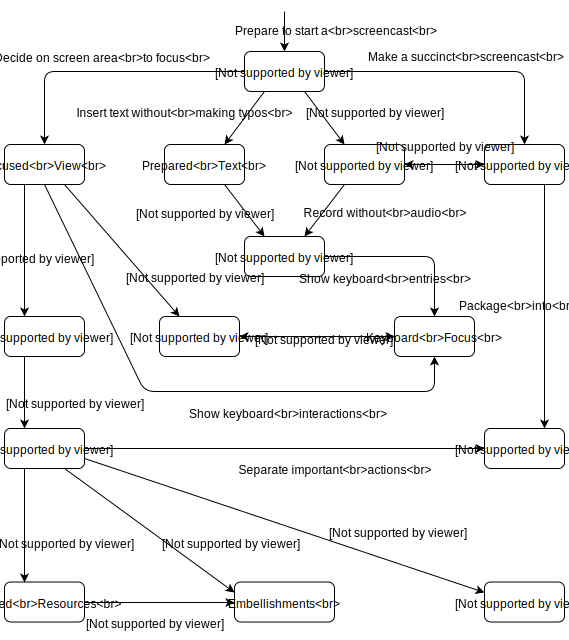
\includegraphics{../../files/screencast.pdf}

Patterns for Screencasting ({[}\protect\hyperlink{Chen2009}{Chen2009}{]})

{[}\protect[\hyperlink{b:Guo2014}{Guo2014}]{]} measured engagement by looking at how long learners
watched MOOC videos. Some of its key findings were:

\begin{itemize}
\item
  Shorter videos are much more engaging---videos should be no more than
  six minutes long.
\item
  A talking head superimposed on slides is more engaging than voice
  over slides alone.
\item
  Videos that felt personal could be more engaging than high-quality
  studio recordings, so filming in informal settings could work better
  than professional studio work for lower cost.
\item
  Drawing on a tablet is more engaging than PowerPoint slides or code
  screencasts, though it's not clear whether this is because of the
  motion and informality, or because it reduces the amount of text on
  the screen.
\item
  It's OK for teachers to speak fairly fast as long as they are
  enthusiastic.
\end{itemize}

One thing {[}\protect[\hyperlink{b:Guo2014}{Guo2014}]{]} didn't address is the chicken-and-egg
problem: do learners find a certain kind of video engaging because
they're used to it, so producing more videos of that kind will
increase engagement simply because of a feedback loop? Or do these
recommendations reflect some deeper cognitive processes? Another thing
this paper didn't look at is learning outcomes: we know that learner
evaluations of courses don't correlate with learning
{[}\protect[\hyperlink{b:Star2014}{Star2014}],\protect[\hyperlink{b:Uttl2017}{Uttl2017}]{]}, and while it's plausible that
learners won't learn from things they don't watch, it remains to be
proven that they \emph{do} learn from things they \emph{do} watch.

\begin{quote}\setlength{\parindent}{0pt}
\textbf{I'm a Little Uncomfortable}

{[}\protect[\hyperlink{b:Guo2014}{Guo2014}]{]}'s research was approved by a university research
ethics board, the learners whose viewing habits were monitored almost
certainly clicked ``agree'' on a terms of service agreement at some
point, and I'm glad to have these insights. On the other hand, I
attended the conference at which this paper was published, and the
word ``privacy'' didn't appear in the title or abstract of \emph{any} of the
dozens of papers or posters presented. Given a choice, I'd rather not
know how engaged learners are than see privacy become obsolete.
\end{quote}

There are many different ways to record video lessons; to find out which
are most effective, {[}\protect[\hyperlink{b:Mull2007a}{Mull2007a}]{]} assigned 364 first-year physics
learners to online multimedia treatments of Newton's First and Second
Laws in one of four styles:

\begin{description}
\tightlist
\item[Exposition:]
concise lecture-style presentation.
\item[Extended Exposition:]
as above with additional interesting information.
\item[Refutation:]
Exposition with common misconceptions explicitly stated and refuted.
\item[Dialog:]
Learner-tutor discussion of the same material as in the Refutation.
\end{description}

Refutation and Dialogue produced the greatest learning gains compared to
Exposition; learners with low prior knowledge benefited most, and those
with high prior knowledge were not disadvantaged.

\section{Flipped Classrooms}\label{s:online-flipped}

Fully automated teaching is one way to use the web in teaching; in
practice, almost all learning in affluent societies has an online
component: sometimes officially, and if not, through peer-to-peer back
channels and surreptitious searches for answers to homework questions.
Combining live and automated instruction allows instructors to use the
strengths of both. In a classroom, the instructor can answer questions
immediately, but it takes time for learners to get feedback on their
coding exercises (sometimes days or weeks). Online, it can take a long
time to get an answer, but learners can get immediate feedback on their
coding (at least for those kinds of exercises we can auto-grade).

Similarly, online exercises have to be more detailed because they're
anticipating questions. I find that in-person lessons start with the
intersection of what everyone needs to know and expands on demand, while
online lessons have to include the union of what everyone needs to know
because you aren't there to do the expanding.

The most popular hybrid teaching strategy today is the
\protect\hyperlink{g:flipped-classroom}{flipped classroom}, in which learners
watch recorded lessons on their own, and class time is used for
discussion and to work through problem sets. Originally proposed in
{[}\protect[\hyperlink{b:King1993}{King1993}]{]}, the idea was popularized as part of peer instruction
(\protect\hyperlink{SECTION}{s:classroom-peer}), and has been studied intensively over
the past decade. For example, {[}\protect[\hyperlink{b:Camp2016}{Camp2016}]{]} compared students who
chose to take a CS1 class online with those who took it in person in a
flipped classroom. Completion of (unmarked) practice exercises
correlated with exam scores for both, but the completion rate of
rehearsal exercises by online students was significantly lower than
lecture attendance rates for in-person students. Looking at what did
affect the grade, they found that the students' perception of the
material's intrinsic value was only a factor for the flipped section
(and only once results were controlled for prior programming
experience). Conversely, test anxiety and self-efficacy were factors
only for the online section; the authors recommend trying to improve
self-efficacy by increasing instructor presence online.

But are lectures worth attending at all? Or should we just provide
recordings? {[}\protect[\hyperlink{b:Nord2017}{Nord2017}]{]} examined the impact of recordings on both
lecture attendance and students' performance at different levels. In
most cases the study found no negative consequences of making recordings
available; in particular, students don't skip lectures when recordings
are available (at least, not any more than they usually do). The
benefits of providing recordings are greatest for students early in
their careers, but diminish as students become more mature.

\section{Life Online}\label{s:online-engagement}

{[}\protect[\hyperlink{b:Nuth2007}{Nuth2007}]{]} found that there are three overlapping worlds in
every classroom: the public (what the teacher is saying and doing), the
social (peer-to-peer interactions between learners), and the private
(inside each learner's head). Of these, the most important is usually
the social: learners pick up as much via cues from their peers as they
do from formal instruction.

The key to making any form of online teaching effective is therefore to
facilitate peer-to-peer interactions. To aid this, courses almost always
have some kind of discussion forum. {[}\protect[\hyperlink{b:Vell2017}{Vell2017}]{]} analyzes
discussion forum posts from 395 CS2 students at two universities by
dividing them into four categories:

\begin{description}
\tightlist
\item[Active:]
request for help that does not display reasoning and doesn't display
what the student has already tried or already knows.
\item[Constructive:]
reflect students' reasoning or attempts to construct a solution to
the problem.
\item[Logistical:]
course policies, schedules, assignment submission, etc.
\item[Content clarification:]
request for additional information that doesn't reveal the student's
own thinking.
\end{description}

They found that constructive and logistical questions dominated, and
that constructive questions correlated with grades. They also found that
students rarely ask more than one active question in a course, and that
these \emph{don't} correlate with grades. While this is disappointing,
knowing it helps set instructors' expectations: while we might all want
our courses to have lively online communities, most won't.

Learners use forums in very different ways, and with very different
results. {[}\protect[\hyperlink{b:Mill2016a}{Mill2016a}]{]} observed that, ``\ldots{}procrastinators are
particularly unlikely to participate in online discussion forums, and
this reduced participation, in turn, is correlated with worse
grades. A possible explanation for this correlation is that
procrastinators are especially hesitant to join in once the discussion
is under way, perhaps because they worry about being perceived as
newcomers in an established conversation. This aversion to jump in
late causes them to miss out on the important learning and motivation
benefits of peer-to-peer interaction.''

\begin{quote}\setlength{\parindent}{0pt}
\textbf{Co-opetition}

{[}\protect[\hyperlink{b:Gull2004}{Gull2004}]{]} describes an innovative online coding contest that
combines collaboration and competition. The contest starts when a
problem description is posted along with a correct, but inefficient,
solution. When it ends, the winner is the person who has made the
greatest overall contribution to improving the performance of the
overall solution. All submissions are in the open, so that
participants can see one another's work and borrow ideas from each
other; as the paper shows, the final solution is almost always a
hybrid borrowing ideas from many people.

{[}\protect[\hyperlink{b:Batt2018}{Batt2018}]{]} described a small-scale variation of this used in
an introductory computing class. In stage one, each student submitted
a programming project individually. In stage two, students were paired
to create an improved solution to the same problem. The assessment
indicates that two-stage projects tend to improve students'
understanding, and that they enjoyed the process.
\end{quote}

Discussion isn't the only way to get students to work together online.
{[}\protect[\hyperlink{b:Pare2008}{Pare2008}]{]} and {[}\protect[\hyperlink{b:Kulk2013}{Kulk2013}]{]} report experiments in which
learners grade each other's work, and the grades they assign are then
compared with grades given by graduate-level teaching assistants or
other experts. Both found that student-assigned grades agreed with
expert-assigned grades as often as the experts' grades agreed with each
other, and that a few simple steps (such as filtering out obviously
unconsidered responses or structuring rubrics) decreased disagreement
even further. And as discussed in \protect\hyperlink{SECTION}{s:individual-peer},
collusion and bias are \emph{not} significant factors in peer grading.

{[}\protect[\hyperlink{b:Cumm2011}{Cumm2011}]{]} looked at the use of shareable feedback tags on
homework; students could attach tags to specific locations in coding
assignments (like code review) so that there's no navigational cost for
the reader, and they controlled whether to share their work and feedback
anonymously. Students found tag clouds of feedback on their own work
useful, but that the tags were really only meaningful in context. This
is unsurprising: the greater the separation between action and feedback,
the greater the cognitive load. What wasn't expected was that the best
and worst students were more likely to share than middling students.

\begin{quote}\setlength{\parindent}{0pt}
\textbf{Trust, but Educate}

The most common way to measure the validity of feedback is to compare
students' grades to experts' grades, but calibrated peer review
(\protect\hyperlink{SECTION}{s:individual-peer}) can be equally effective. Before
asking learners to grade each others' work, they are asked to grade
samples and compare their results with the grades assigned by the
teacher. Once the two align, the learner is allowed to start giving
grades to peers. Given that critical reading is an effective way to
learn, this result may point to a future in which learners use
technology to make judgments, rather than being judged by technology.
\end{quote}

One technique we will definitely see more of in coming years is online
streaming of live coding sessions {[}\protect[\hyperlink{b:Haar2017}{Haar2017}]{]}. This has most of
the benefits discussed in \protect\hyperlink{SECTION}{s:performance-live}, and when
combined with collaborative note-taking
(\protect\hyperlink{SECTION}{s:classroom-notetaking}) it can come pretty close to
approximating an in-class experience.

Looking even further ahead, {[}\protect[\hyperlink{b:Ijss2000}{Ijss2000}]{]} identified four levels of
online presence, from realism (we can't tell the difference) through
immersion (we forget the difference) and involvement (we're engaged but
aware of the difference) to suspension of disbelief (we are doing most
of the work). Crucially, they distinguish physical presence, which is
the sense of actually being somewhere, and social presence, which is the
sense of being with others. In most learning situations, the latter is
more important, and one way to foster it is to bring the technology
learners use every day into the classroom. For example,
{[}\protect[\hyperlink{b:Deb2018}{Deb2018}]{]} found that doing in-class exercises with realtime
feedback using mobile devices improved concept retention and student
engagement while reducing failure rates.

\begin{quote}\setlength{\parindent}{0pt}
\textbf{Hybrid Presence}

Combining online and in-person instruction can be more effective than
either on its own. I have delivered very successful classes using
real-time remote instruction, in which the learners are co-located at
2--6 sites, with helpers present, while I taught via streaming video
(\protect\hyperlink{SECTION}{s:joining-using}). This scales well, saves on travel
costs, and is less disruptive for learners (particularly those with
family responsibilities). What \emph{doesn't} work is having one group in
person and one or more groups remotely: with the best will in the
world, the local participants get far more attention.
\end{quote}

Online teaching is still in its infancy: {[}\protect[\hyperlink{b:Luxt2009}{Luxt2009}]{]} surveyed
peer assessment tools that could be useful in computing education, and
{[}\protect[\hyperlink{b:Broo2016}{Broo2016}]{]} describes many other ways groups can discuss things,
but only a handful of these ideas are widely known or used.

\begin{quote}\setlength{\parindent}{0pt}
I think that our grandchildren will probably regard the distinction we
make between what we call the real world and what they think of as
simply the world as the quaintest and most incomprehensible thing
about us.

--- William Gibson
\end{quote}

\section{Exercises}\label{s:online-exercises}

\subsection{Give Feedback on a Bad Screencast (whole class/20)}\label{give-feedback-on-a-bad-screencast-whole-class20}

Watch \href{https://youtu.be/xcnoHaxXvdQ}{this screencast} as a group and give
feedback on it. Organize feedback along two axes: positive
vs. negative and content vs. presentation. When you are done, have
each person in the class add one point to a 2x2 grid on a whiteboard
(or in the shared notes) without duplicating any points that are
already up there. What did other people see that you missed? What did
they think that you strongly agree or disagree with? (You can compare
your answers with the checklist in \protect\hyperlink{APPENDIX}{s:teacheval}.)

\subsection{Two-Way Video (pairs/10)}\label{two-way-video-pairs10}

Record a 2--3 minute video of yourself doing something, then swap
machines with a partner so that each of you can watch the other's video
at 4X speed. How easy is it to follow what's going on? What if anything
did you miss?

\subsection{Viewpoints (individual/10)}\label{viewpoints-individual10}

According to {[}\protect[\hyperlink{b:Irib2009}{Irib2009}]{]}, different disciplines focus on
different factors affecting the success or otherwise of online
communities:

\begin{description}
\tightlist
\item[Business:]
customer loyalty, brand management, extrinsic motivation.
\item[Psychology:]
sense of community, intrinsic motivation.
\item[Sociology:]
group identity, physical community, social capital, collective
action.
\item[Computer Science:]
technological implementation.
\end{description}

Which of these perspectives most closely corresponds to your own? Which
are you least aligned with?

\subsection{Helping or Harming (small groups/30)}\label{helping-or-harming-small-groups30}

\href{https://www.nytimes.com/2018/01/19/business/online-courses-are-harming-the-students-who-need-the-most-help.html}{Susan Dynarski's article in the \emph{New York
Times}} explains how and why schools are
putting students who fail in-person courses into online courses, and
how this sets them up for even further failure.

\begin{enumerate}
\item
  Working in small groups, read the article, come up with 2--3 things
  that schools could do to compensate for these negative effects, and
  create rough estimates of their per-student costs.
\item
  Compare your suggestions and costs with those of other groups. How
  many full-time teaching positions do you think would have to be cut
  in order to free up resources to implement the most popular ideas
  for 100 students?
\item
  As a class, do you think that would be a net benefit for the
  students or not?
\end{enumerate}

Budgeting exercises like this are a good way to tell who's serious about
educational change. Everyone can think of things they'd like to do; far
fewer are willing to talk about the tradeoffs needed to make change
happen.

\chapter{Exercise Types}\label{s:exercises}

Every good carpenter has a set of screwdrivers, and every good teacher
has different kinds of formative assessment exercises to check what
learners are actually learning, help them practice their new skills, and
keep them engaged. This chapter starts by describing several kinds of
exercises you can use to check if your teaching has been effective. It
then looks at the state of the art in automated grading, and closes by
exploring discussion, projects, and other important kinds of work that
require more human attention to assess. Our discussion draws in part on
the \href{http://web-cat.org/questionbank/}{Canterbury Question Bank}
{[}\protect[\hyperlink{b:Sand2013}{Sand2013}]{]}, which has entries for various languages and topics
in introductory computing.

\section{The Classics}\label{s:exercises-classics}

As \protect\hyperlink{SECTION}{s:models-formative-assessment} discussed, \emph{multiple
choice questions} (MCQs) are most effective when the wrong answers probe
for specific misconceptions. In terms of Bloom's Taxonomy
(\protect\hyperlink{SECTION}{s:process-objectives}), MCQs are usually designed to test
recall and understanding (``What is the capital of Saskatchewan?''), but
they can also require learners to exercise judgment.

\begin{quote}\setlength{\parindent}{0pt}
\textbf{A Multiple Choice Question}

In what order do operations occur when the computer evaluates the
expression \texttt{price\ =\ addTaxes(cost\ -\ discount)}?

\begin{enumerate}
\tightlist
\item
  subtraction, function call, assignment
\item
  function call, subtraction, assignment
\item
  function call, then assignment and subtraction simultaneously
\item
  none of the above
\end{enumerate}
\end{quote}

The second classic type of programming exercise is \emph{code and run}
(C\&R), in which the learner writes code that produces a specified
output. C\&R exercises can be as simple or as complex as the teacher
wants, but for in-class use, they should be brief and have only one or
two plausible correct answers. For novices, it's often enough to ask
them to call a specific function: experienced teachers often forget how
hard it can be to figure out which parameters go where. For more
advanced learners, figuring out which function to call is more engaging
and a better gauge of their understanding.

\begin{quote}\setlength{\parindent}{0pt}
\textbf{Code \& Run}

The variable \texttt{picture} contains a full-color image read from a file.
Using one function, create a black and white version of the image and
assign it to a new variable called \texttt{monochrome}.
\end{quote}

Write and run exercises can be combined with MCQs. For example, this MCQ
can only be answered by running the Unix \texttt{ls} command:

\begin{quote}\setlength{\parindent}{0pt}
\textbf{Combining MCQ with Code \& Run}

You are in the directory \texttt{/home/greg}. Which of the following files is
\emph{not} in that directory?

\begin{enumerate}
\tightlist
\item
  \texttt{autumn.csv}
\item
  \texttt{fall.csv}
\item
  \texttt{spring.csv}
\item
  \texttt{winter.csv}
\end{enumerate}
\end{quote}

C\&Rs help learners practice the skills they most want to learn, but
they can be hard to assess: learners can find lots of unexpected ways to
get the right answer, and are demoralized if an automatic grading system
rejects their code because it doesn't match the instructor's. One way to
reduce how often this occurs is to assess only their output, but that
doesn't give them feedback on how they are programming. Another is to
give them a small test suite they can run their code against before they
submit it (at which point it is run against a more comprehensive set of
tests). Doing this helps them figure out if they have completely
misunderstood the intent of the exercise before they do anything that
they think might cost them grades.

Instead of writing code that satisfies some specification, learners can
be asked to write tests to determine whether a piece of code conforms to
a spec. This is a useful skill in its own right, and doing it may give
students a bit more sympathy for how hard their teachers work.

\begin{quote}\setlength{\parindent}{0pt}
\textbf{Inverting Code \& Run}

The function \texttt{monotonic\_sum} calculates the sum of each section of a
list of numbers in which the values are strictly increasing. For
example, given the input \texttt{{[}1,\ 3,\ 3,\ 4,\ 5,\ 1{]}}, the output is
\texttt{{[}4,\ 12,\ 1{]}}. Write and run unit tests to determine which of the
following bugs the function contains:

\begin{itemize}
\item
  Considers every negative number the start of a new sub-sequence.
\item
  Does not include the first value of each sub-sequence in the
  sub-sum.
\item
  Does not include the last value of each sub-sequence in the
  sub-sum.
\item
  Only re-starts the sum when values decrease rather than fail to
  increase.
\end{itemize}
\end{quote}

\emph{Fill in the blanks} is a refinement of C\&R in which the learner is
given some starter code and has to complete it. (In practice, most C\&R
exercises are actually fill in the blanks because the teacher will
provide comments to remind the learners of the steps they should take.)
As discussed in \protect\hyperlink{CHAPTER}{s:load}, novices often find filling in the
blanks less intimidating than writing all the code from scratch, and
since the teacher has provided most of the answer's structure,
submissions are much more predictable and therefore easier to check.

\begin{quote}\setlength{\parindent}{0pt}
\textbf{Fill in the Blanks}

Fill in the blanks so that the code below prints the string \texttt{\textquotesingle{}hat\textquotesingle{}}.

\begin{lstlisting}
text = 'all that it is'
slice = text[____:____]
print(slice)
\end{lstlisting}
\end{quote}

As described in \protect\hyperlink{CHAPTER}{s:load}, \protect\hyperlink{g:parsons-problem}{Parsons
Problems} also avoid the ``blank screen of terror''
problem. The learner is given the lines of code needed to solve a
problem, but has to put them in the right order. Research over the
past few years has shown that Parsons Problems are effective because
they allow learners to concentrate on control flow separately from
vocabulary
{[}\protect[\hyperlink{b:Pars2006}{Pars2006}],\protect[\hyperlink{b:Eric2015}{Eric2015}],\protect[\hyperlink{b:Morr2016}{Morr2016}],\protect[\hyperlink{b:Eric2017}{Eric2017}]{]}. The
same research shows that giving the learner more lines than she needs,
or asking her to rearrange some lines and add a few more, makes this
kind of problem significantly harder {[}\protect[\hyperlink{b:Harm2016}{Harm2016}]{]}. Tools for
building and doing Parsons Problems online exist {[}\protect[\hyperlink{b:Ihan2011}{Ihan2011}]{]},
but they can be emulated (albeit somewhat clumsily) by asking learners
to rearrange lines of code in an editor.

\begin{quote}\setlength{\parindent}{0pt}
\textbf{Parsons Problem}

Rearrange and indent these lines to sum the positive values in a list.
(You will need to add colons in appropriate places as well.)

\begin{lstlisting}
total = 0
if v > 0
total += v
for v in values
\end{lstlisting}
\end{quote}

\section{Tracing}\label{s:exercises-tracing}

\emph{Tracing execution} is the inverse of a Parsons Problem: given a few
lines of code, the learner has to trace the order in which those lines
are executed. This is an essential debugging skill, and is a good way to
solidify learners' understanding of loops, conditionals, and the
evaluation order of function and method calls. The easiest way to
implement it is to have learners write out a sequence of labelled steps.
Having them choose the correct sequence from a set (i.e., presenting
this as an MCQ) adds cognitive load without adding value, since they
have to do all the work of figuring out the correct sequence, then
search for it in the list of options.

\begin{quote}\setlength{\parindent}{0pt}
\textbf{Tracing Execution Order}

In what order are the labelled lines in this block of code executed?

\begin{lstlisting}
A)     vals = [-1, 0, 1]
B)     inverse_sum = 0
       try:
           for v in vals:
C)             inverse_sum += 1/v
       except:
D)         pass
\end{lstlisting}
\end{quote}

\emph{Tracing values} is similar to tracing execution, but instead of
spelling out the order in which code is executed, the learner has to
list the values that one or more variables take on as the program runs.
It can also be implemented by having learners provide a list of values,
but another approach is to give the learner a table whose columns are
labelled with variable names and whose rows are labelled with line
numbers, and asking them to fill in all of the values taken on by all of
the variables.

\begin{quote}\setlength{\parindent}{0pt}
\textbf{Tracing Values}

What values do \texttt{left} and \texttt{right} take on as this program executes?

\begin{lstlisting}
left = 24
right = 6
while right:
    left, right = right, left % right
\end{lstlisting}
\end{quote}

You can also require learners to trace code backwards, e.g., to figure
out what the input must have been if the code produced a particular
result {[}\protect[\hyperlink{b:Armo2008}{Armo2008}]{]}. These \emph{reverse execution} problems require
search and deductive reasoning, but they are particularly useful when
the ``output'' is an error message, and help learners develop valuable
debugging skills.

\begin{quote}\setlength{\parindent}{0pt}
\textbf{Reverse Execution}

Fill in the missing number in \texttt{values} that caused this function to
crash.

\begin{lstlisting}
values = [ [1.0, -0.5], [3.0, 1.5], [2.5, ___] ]
runningTotal = 0.0
for (reading, scaling) in values:
    runningTotal += reading / scaling
\end{lstlisting}
\end{quote}

\emph{Minimal fix} exercises also help learners develop debugging skills.
Given a few lines of code that contain a bug, the learner must either
make or identify the smallest change that will produce the correct
output. Making the change can be done using C\&R, while identifying it
can be done as a multiple choice question.

\begin{quote}\setlength{\parindent}{0pt}
\textbf{Minimal Fix}

This function is supposed to test whether a number lies within a
range. Make one small change so that it actually does so.

\begin{lstlisting}
def inside(point, lower, higher):
    if (point <= lower):
        return false
    elif (point <= higher):
        return false
    else:
        return true
\end{lstlisting}
\end{quote}

\emph{Theme and variation} exercises are similar, but instead of making a
change to fix a bug, the learner is asked to make a small alteration
that changes the output in some specific way. Allowed changes can
include replacing one function call with another, changing one
variable's initial value, swapping an inner and outer loop, changing
the order of tests in a chain of conditionals, or changing the nesting
of function calls or the order in which methods are chained. Again, this
kind of exercise gives learners a chance to practice a useful real-world
skill: the fastest way to produce a working program is often to tweak
one that already does something useful.

\begin{quote}\setlength{\parindent}{0pt}
\textbf{Theme and Variations}

Change the inner loop in the function below so that it fills the upper
left triangle of an image with a specified color.

\begin{lstlisting}
function fillTriangle(picture, color) is
    for x := 1 to picture.width do
        for y := 1 to picture.height do
            picture[x, y] = color
        end
    end
end
\end{lstlisting}
\end{quote}

\emph{Refactoring exercises} are the complement of theme and variation
exercises: given a working piece of code, the learner has to modify it
in some way \emph{without} changing its output. For example, the learner
could be asked to replace loops with vectorized expressions, to simplify
the condition in a while loop, etc. The exercise here is that there are
often so many ways to refactor a piece of code that grading requires
human intervention.

\begin{quote}\setlength{\parindent}{0pt}
\textbf{Refactoring}

Write a single list comprehension that has the same effect as this
loop.

\begin{lstlisting}
result = []
for v in values:
    if len(v) > threshold:
        result.append(v)
\end{lstlisting}
\end{quote}

\section{Diagrams}\label{s:exercises-diagrams}

Having students draw concept maps and other diagrams gives insight into
how they're thinking (\protect\hyperlink{SECTION}{s:memory-concept-maps}), but free-form
diagrams take human time and judgment to assess. \emph{Labelling diagrams},
on the other hand, is almost as useful from a pedagogical point of view
but much easier to scale.

Rather than having learners create diagrams from scratch, provide them
with a diagram and a set of labels and have them put the latter in the
right places on the former. The diagram can be a complex data structure
(``after this code is executed, which variables point to which parts of
this structure?''), the graph that a program produces (``match each of
these pieces of code with the part of the graph it generated''), the code
itself (``match each term to an example of that program element''), or
many other things; the key is that constraining the set of solutions
makes this usable in class and at scale.

\begin{quote}\setlength{\parindent}{0pt}
\textbf{Labelling a Diagram}

The tree below shows how a small fragment of HTML is represented in
memory. Put the labels 1--10 on the elements of the tree to show the
order in which they are reached in a depth-first traversal.

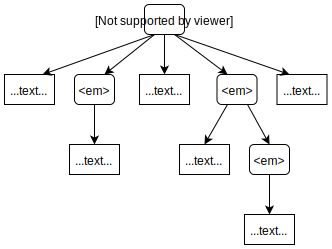
\includegraphics{../../files/labelling.pdf}
\end{quote}

Another way to use diagrams for formative assessment is to give learners
the pieces of the diagram and ask them to arrange them correctly. This
is a visual equivalent of a Parsons Problem, and you can provide as much
or as little of a skeleton to help them with placement as you think
they're ready for. (I have fond memories of trying to place resistors
and capacitors in a circuit diagram in order to get the right voltage at
a certain point, and have often seen teachers give learners a fixed set
of Scratch blocks and ask them to create a particular drawing using only
those blocks.)

\emph{Matching problems} can be thought of as a special case of labelling in
which the ``diagram'' is a column of text and the labels are taken from
the other column. \emph{One-to-one matching} gives the learner two lists of
equal length and asks her to pair corresponding items, e.g., ``match each
piece of code with the output it produces''.

\begin{quote}\setlength{\parindent}{0pt}
\textbf{Matching}

Match each regular expression operator with what it does.

\begin{longtable}[]{@{}ll@{}}
\toprule
\texttt{?} & start of line\tabularnewline
\texttt{*} & zero or one occurrences\tabularnewline
\texttt{+} & end of line\tabularnewline
\texttt{\$} & one or more occurrences\tabularnewline
\texttt{\^{}} & zero or more occurrences\tabularnewline
\bottomrule
\end{longtable}
\end{quote}

\emph{Many-to-many matching} is similar, but the lists aren't the same
length, so some items may be matched to several others, while others may
not be matched at all. Both kinds require learners to use higher-order
thinking skills, but many-to-many are more difficult because learners
can't do easy matches first to reduce their search space (i.e., there is
a higher cognitive load.)

Matching problems can be implemented by having learners submit lists of
matching pairs as text (such as ``A3, B1, C2''), but that's clumsy and
error-prone. Having them recognize a set of correct pairs in an MCQ is
even worse, as it's painfully easy to misread.

\emph{Ranking} is a special case of matching that is (slightly) more amenable
to answering via lists, since our minds are pretty good at detecting
errors or anomalies in sequences. Give the learner several items and ask
them to order them from fastest to slowest, most robust to most brittle,
and so on. The former tends toward recall (e.g., recognizing the names
of various sorting algorithms and knowing their properties), while the
latter tends more toward reasoning and judgment.

\emph{Summarization} also requires learners to use higher-order thinking, and
gives them a chance to practice a skill that is very useful when
reporting bugs rather than fixing them. For example, learners can be
asked, ``Which sentence best describes how the output of f changes as x
varies from 0 to 10?'' and then given several options as a multiple
choice question.

You can also ask for very short free-form answers to questions in
constrained domains, e.g., ``What is the key feature of a stable sorting
algorithm?'' We still can't fully automate checks for these without a
frustrating number of false positives (accepting wrong answers) and
false negatives (rejecting correct ones), but they lend themselves well
to peer grading (\protect\hyperlink{SECTION}{s:individual-peer}).

\section{Automatic Grading}\label{s:exercises-grading}

Automatic program grading tools have been around longer than I've been
alive: the earliest published mention dates from 1960
{[}\protect[\hyperlink{b:Holl1960}{Holl1960}]{]}, and the surveys published in
{[}\protect[\hyperlink{b:Douc2005}{Douc2005}],\protect[\hyperlink{b:Ihan2010}{Ihan2010}]{]} mention many specific tools by name.
Building such tools is a lot more complex than it might first seem. How
are assignments represented? How are submissions tracked and reported?
Can learners co-operate? How can submissions be executed safely?
{[}\protect[\hyperlink{b:Edwa2014a}{Edwa2014a}]{]} is an entire paper devoted to an adaptive scheme for
detecting and managing infinite loops and other non-terminating code
submissions, and that's just one of the many issues that comes up.

As elsewhere, it's important to distinguish learner satisfaction from
learning outcomes. {[}\protect[\hyperlink{b:Magu2018}{Magu2018}]{]} switched informal programming labs
to a weekly machine-evaluated test for a second-year CS course using an
auto-grading tool originally developed for programming competitions.
Learners didn't like the automated system, but the overall failure rate
for the course was halved, and the number of learners gaining first
class honors tripled. In contrast, {[}\protect[\hyperlink{b:Rubi2014}{Rubi2014}]{]} also began to use
an auto-grader designed for competitions, but saw no significant
decrease in their learners' dropout rates; once again, learners made
some negative comments about the tool, which the authors attribute to
its feedback messages rather than to dislike of auto-grading.

{[}\protect[\hyperlink{b:Srid2016}{Srid2016}]{]} took a different approach. They used
\protect\hyperlink{g:fuzz-testing}{fuzz testing} (i.e., randomly-generated
test cases) to check whether learner code does the same thing as a
reference implementation supplied by the teacher. In the first project
of a 1400-learner introductory course, fuzz testing caught errors that
were missed by a suite of hand-written test cases for more than 48\% of
learners, which clearly demonstrates its value.

{[}\protect[\hyperlink{b:Basu2015}{Basu2015}]{]} gave learners a suite of solution test cases, but
learners had to unlock each one by answering questions about its
expected behavior before they were allowed to apply it to their proposed
solution. For example, suppose learners are writing a function to find
the largest adjacent pair of numbers in a list; before being allowed to
use the tests associated with this question, they have to choose the
right answer to, ``What does \texttt{largestPair(4,\ 3,\ -1,\ 5,\ 3,\ 3)} produce?''
(The correct answer is \texttt{(5,\ 3)}.) In a 1300-person university course,
the vast majority of learners chose to validate their understanding of
test cases this way before attempting to solve problems, and then asked
fewer questions and expressed less confusion about assignments.

It's tempting to use off-the-shelf style checking tools to grade
learners' code. However, {[}\protect[\hyperlink{b:Nutb2016}{Nutb2016}]{]} initially found no
correlation between human-provided marks and style-checker rule
violations. Sometimes this was because learners violated one rule many
times (thereby losing more points than they should have), and other
times it was because they submitted the assignment starter code with few
alterations and got more points than they should have.

{[}\protect[\hyperlink{b:Buff2015}{Buff2015}]{]} presents a well-informed reflection on
the whole idea of providing automated feedback. Their starting point
is that, ``Automated grading systems help learners identify bugs in
their code, {[}but{]} may inadvertently discourage learners from thinking
critically and testing thoroughly and instead encourage dependence on
the teacher's tests.'' One of the key issues they identified is that a
learner may thoroughly test their code, but the feature may still not
be implemented according to the teacher's specifications. In this
case, the ``failure'' is not caused by a lack of testing, but by a
misunderstanding of the requirements, and it is unlikely that more
testing will expose the problem. If the auto-grading system doesn't
provide insightful, actionable feedback, this experience will only
frustrate the learner.

In order to provide that feedback, {[}\protect[\hyperlink{b:Buff2015}{Buff2015}]{]}'s system
identifies which method or methods of the learner's code are executed by
failing tests, so that the system can associate failed tests with
particular features within the learner's submission. The system decides
whether specific hints have been ``earned'' by seeing whether the learner
has tested the associated feature enough, so learners cannot rely on
hints instead of doing tests.

{[}\protect[\hyperlink{b:Keun2016a}{Keun2016a}],\protect[\hyperlink{b:Keun2016b}{Keun2016b}]{]} classified the messages produced by 69
auto-grading tools. They found that these often do not give feedback on
how to fix problems and take the next step. They also found that most
teachers cannot easily adapt most of the tools to their needs; like many
workflow tools, they tend to enforce their creators' unrecognized
assumptions about how institutions work. Their work is ongoing, and
their detailed classification scheme is a useful shopping list when
looking at tools of this kind.

{[}\protect[\hyperlink{b:Srid2016}{Srid2016}]{]} discussed strategies for sharing feedback with
learners when automatically testing their code. The first is to provide
the expected output for the tests---but then learners hard-code output for
those inputs (because anything that can be gamed, will be). An
alternative is to report the pass/fail results for the learners' code,
but only supply the actual inputs and outputs of the tests after the
submission date. This can be frustrating, because it tells learners they
are wrong, but not why.

A third option is to use a technique called \protect\hyperlink{g:hashing}{hashing} to
generate a value that depends on the output, but doesn't reveal it. If
the user produces exactly the same output, its hash will be the same
as the hash of the correct output, which will unlock the solution, but
it is impossible to work backward from the hash to figure out what the
output is supposed to be. Hashing is used to create digital signatures
for documents, and requires a bit more work and explanation to set up,
but strikes a good balance between revealing answers prematurely and
not revealing them when it would help.

\section{Higher-Level Thinking}\label{s:exercises-higher}

Many other kinds of programming exercises are hard for teachers to
assess in a class with more than few dozen learners, and equally hard
for automated platforms to assess at all. Larger programming projects,
or projects in which learners set their own goals, are (hopefully) what
classes are building toward. Free-form discussion or twitch coding
(\protect\hyperlink{SECTION}{s:performance-live}) is also valuable, but also doesn't
scale.

\emph{Code review}, on the other hand, is hard to grade automatically in the
general case, but can be tackled if learners are given a rubric (e.g., a
list of faults to look for) and asked to match particular comments
against particular lines of code. For example, the learner can be told
that there are two indentation errors and one bad variable name, and
asked to point them out; if she is more advanced, she could be given
half a dozen kinds of remarks she could make about the code without
guidance as to how many of each she should find.

{[}\protect[\hyperlink{b:Steg2016b}{Steg2016b}]{]} is a good starting point for a code style rubric,
while {[}\protect[\hyperlink{b:Luxt2009}{Luxt2009}]{]} looks at peer review in programming classes
more generally. If you are going to have students do reviews, use
calibrated peer review (\protect\hyperlink{SECTION}{s:individual-peer}) so that they
have models of what good feedback should look like.

\begin{quote}\setlength{\parindent}{0pt}
\textbf{Code Review}

Using the rubric provided, mark each line of the code below.

\begin{lstlisting}
01)  def addem(f):
02)      x1 = open(f).readlines()
03)      x2 = [x for x in x1 if x.strip()]
04)      changes = 0
05)      for v in x2:
06)          print('total', total)
07)          tot = tot + int(v)
08)      print('total')
\end{lstlisting}

\begin{enumerate}
\tightlist
\item
  poor variable name
\item
  unused variable
\item
  use of undefined variable
\item
  missing return value
\end{enumerate}
\end{quote}

\section{Exercises}\label{s:exercises-exercises}

\subsection{Code and Run (pairs/10)}\label{code-and-run-pairs10}

Create a short C\&R exercise; trade with a partner, and see how long it
takes each of you to understand and do the other's exercise. Were there
any ambiguities or misunderstandings in the exercise description?

\subsection{Inverting Code and Run (small groups/15)}\label{inverting-code-and-run-small-groups15}

Form groups of 4--6 people. Have each member of the group create an
inverted C\&R exercise that requires people to figure out what input
produces a particular output. Pick two at random, and see how many
different inputs the group can find that satisfy the requirements.

\subsection{Tracing Values (pairs/10)}\label{tracing-values-pairs10}

Write a short program (10--15 lines); trade with a partner, and trace how
the variables in the program change value over time. What differences
are there in how you and your partner wrote down your traces?

\subsection{Refactoring (small groups/15)}\label{refactoring-small-groups15}

Form groups of 3--4 people. Have each person select a short piece of code
(10--30 lines long) that they have written that isn't as tidy as it could
be. Choose one at random, and have everyone in the group tidy it up
independently. How do your cleaned-up versions differ? How well or how
poorly would you be able to accommodate all of these variations if
marking automatically or in a large class?

\subsection{Labelling a Diagram (pairs/10)}\label{labelling-a-diagram-pairs10}

Draw a diagram showing something that you have explained recently: how
browsers fetch data from servers, the relationship between objects and
classes, or how data frames are indexed in R. Put the labels on the
side, and ask your partner to place them.

\subsection{Pencil-and-Paper Puzzles (whole class/15)}\label{pencil-and-paper-puzzles-whole-class15}

{[}\protect[\hyperlink{b:Butl2017}{Butl2017}]{]} describes a set of pencil-and-paper puzzles that can
be turned into introductory programming assignments, and found that
these assignments are enjoyed by students and encourage meta-cognition.
Think of a simple pencil-and-paper puzzle or game you played as a child,
and describe how you would turn it into a programming exercise.

\subsection{Counting Failures (pairs/15)}\label{counting-failures-pairs15}

Any useful estimate of how much time an exercise needs must take into
account how frequent failures are and how much time is lost to them. For
example, editing text files seems like a simple task, but what about
finding those files? Most GUI editors save things to the user's desktop
or home directory; if the files used in a course are stored somewhere
else, a substantial fraction won't be able to navigate to the right
directory without help. (If this seems like a small problem to you,
please revisit the discussion of expert blind spot in
\protect\hyperlink{CHAPTER}{s:memory}.)

Working with a partner, make a list of ``simple'' things you have seen go
wrong in exercises you have used or taken. How often do they come up?
How long do they take learners to fix on their own, or with help? How
much time do you currently budget in class to deal with them?

\chapter{Building Community}\label{s:community}

Many well-intentioned people want the world to be a better place, but
don't actually want anything important to change. A lot of grassroots
efforts to teach programming fall into this category: they want to teach
children and adults how to program so that they can get good jobs,
rather than empower them to change the system that has shut them (and
people like them) out of those jobs in the past.

If you are going to build a community, the first and most important
thing you have to decide is what \emph{you} want: to help people succeed in
the world we have, or to give them a way to make a better one. Either
way, you have to accept that one person can only do so much. Just as we
learn best together, we teach best when we are teaching with other
people, and the best way to achieve that is to build a community.

And as Anu Partanen \href{https://www.theatlantic.com/national/archive/2011/12/what-americans-keep-ignoring-about-finlands-school-success/250564/}{pointed out}, sometimes
you need to fix several things in order to fix one. Finland's teachers
aren't successful in isolation: they are able to achieve outstanding
results because their country's citizens truly value equality of
opportunity. People (and countries) that try to adopt their teaching
methods without ensuring that children (and parents) are well
nourished, safe, and treated fairly by the courts will have a more
difficult time. This doesn't mean you have to fix all of society's
ills in order to teach programming, but it \emph{does} mean that you have
to understand and be involved in what happens to your learners outside
of your class if you want that class to work.

A framework in which to think about educational communities is
\protect\hyperlink{g:situated-learning}{situated learning}, which focuses on how
\protect\hyperlink{g:legitimate-peripheral-participation}{legitimate peripheral
participation} leads to people
becoming members of a \protect\hyperlink{g:community-of-practice}{community of
practice} {[}\protect[\hyperlink{b:Weng2015}{Weng2015}]{]}. Unpacking
those terms, a community of practice is a group of people bound
together by interest in some activity, such as knitting or particle
physics. Legitimate peripheral participation means doing simple,
low-risk tasks that community nevertheless recognizes as valid
contributions: making your first scarf, stuffing envelopes during an
election campaign, or proof-reading documentation for open source
software.

Situated learning focuses on the transition from being a newcomer to
being accepted as a peer by those who are already community members.
This typically means starting with simplified tasks and tools, then
doing similar tasks with more complex tools, and finally tackling the
exercises of advanced practitioners. For example, children learning
music may start by playing nursery rhymes on a recorder or ukulele, then
play other simple songs on a trumpet or saxophone in a band, and finally
start exploring their own musical tastes. Healthy communities of
practice understand and support these progressions, and recognize that
each step is meant to give people a ramp rather than a cliff. Some of
the ways they do this include:

\begin{description}
\tightlist
\item[Problem solving:]
``I'm stuck---Can we work on this design and brainstorm some ideas?''
\item[Requests for information:]
``Where can I find the code to connect to the server?''
\item[Seeking experience:]
``Has anyone dealt with a customer in this situation?''
\item[Reusing assets:]
``I have a proposal for an event website that I wrote for a client
last year you can use as a starting point.''
\item[Coordination and synergy:]
``Can we combine our purchases of web hosting to get a discount?''
\item[Building an argument:]
``How do people in other companies do this? Armed with this
information it will be easier to convince my CEO to make some
changes.''
\item[Growing confidence:]
``Before I do it, I'll run it through my community first to see what
they think.''
\item[Discussing developments:]
``What do you think of the new work tracking system? Does it really
help?''
\item[Documenting projects:]
``We have faced this problem five times now. Let us write it down
once and for all.''
\item[Visits:]
``Can we come and see your after-school program? We need to establish
one in our city.''
\item[Mapping knowledge and identifying gaps:]
``Who knows what, and what are we missing? What other groups should
we connect with?''
\end{description}

Whatever the domain, situated learning emphasizes that learning is a
social activity. In order to be effective and sustainable, teaching
therefore needs to be rooted in a community; if one doesn't exist, you
need to build one. There are at least \href{https://www.feverbee.com/types-of-community-and-activity-within-the-community/}{four types}:

\begin{description}
\tightlist
\item[Community of action:]
people focused on a shared goal, such as getting someone elected.
\item[Community of concern:]
members are brought together by a shared exercise, such as dealing
with depression.
\item[Community of interest:]
focused on a shared love of something like backgammon or knitting.
\item[Community of place:]
of people who happen to live or work side by side.
\end{description}

Most real communities are mixes of these, such as people in Toronto who
like teaching tech; what matters is that you pick something and stick
with it.

\section{Learn, Then Do}\label{s:community-learn-then-do}

The first step in building a community is to decide if you really need
to, or whether you would be more effective joining an existing
organization. Thousands of groups are already teaching people tech
skills, from the \href{http://www.4-h-canada.ca/}{4-H Club} and \href{https://www.frontiercollege.ca/}{literacy
programs} to get-into-coding non-profits like \href{http://www.blackgirlscode.com/}{Black
Girls Code} and \href{http://bridgeschool.io/}{Bridge}. Joining an
existing group will give you a head start on teaching, an immediate
set of colleagues, and a chance to learn more about how to run things;
hopefully, learning those skills will be more important than being
able to say that you're the founder or leader of something new.

Whether you join an existing group or set up one of your own, you owe
it to yourself and everyone who's going to work with you to find out
what's been done before. People have been writing about grassroots
organizing for decades; {[}\protect[\hyperlink{b:Alin1989}{Alin1989}]{]} is probably the best-known
work on the subject, while {[}\protect[\hyperlink{b:Brow2007}{Brow2007}],\protect[\hyperlink{b:Midw2010}{Midw2010}]{]} are
practical manuals rooted in decades of practice. If you want to read
more deeply, {[}\protect[\hyperlink{b:Adam1975}{Adam1975}]{]} is a history of the Highlander Folk
School, whose approach has been emulated by many successful groups,
while {[}\protect[\hyperlink{b:Spal2014}{Spal2014}]{]} is a guide to teaching adults written by
someone with deep personal roots in organizing, and
\href{https://www.nonprofitready.org/}{NonprofitReady.org} offers free professional
development training.

\section{Three Steps}\label{s:community-three-steps}

Everyone who gets involved with your organization, including you, goes
through three phases: recruitment, retention, and retirement (from the
organization). You don't need to worry about this cycle when you're just
getting started, but it \emph{is} worth thinking about as soon as you have
more than a couple of non-founders involved.

The first step is recruiting volunteers. Your marketing should help you
with this by making your organization findable, and by making its
mission and its value to volunteers clear to people who might want to
get involved. Share stories that exemplify the kind of help you want as
well as stories about the people you're helping, and make it clear that
there are many ways to get involved. (We discuss this in more detail in
the next section.)

Your best source of new recruits is your own classes: ``see one, do one,
teach one'' has worked well for volunteer organizations for as long as
there have \emph{been} volunteer organizations. Make sure that every class or
other encounter ends with two sentences explaining how people can help,
and that help is welcome. People who come to you this way will know what
you do, and will have recent experience of being on the receiving end of
what you offer that they can draw on, which helps your organization
avoid collective \protect\hyperlink{g:expert-blind-spot}{expert blind spot}.

\begin{quote}\setlength{\parindent}{0pt}
\textbf{Start Small}

As \href{https://en.wikipedia.org/wiki/Ben_Franklin_effect}{Ben Franklin} observed, a person who has
performed a favor for someone is more likely to do another favor for
that person than they would be if they had received a favor from
that person. Asking people to do something small for you is
therefore a good step toward getting them to do something
larger. One natural way to do this when teaching is to ask people to
submit fixes for your lesson materials for typos or unclear wording,
or to suggest new exercises or examples. If your materials are
written in a maintainable way
(\protect\hyperlink{SECTION}{s:process-maintainability}), this gives them a chance to
practice some useful skills, and gives you an opportunity to start a
conversation that might lead to a new recruit.
\end{quote}

Recruiting doesn't end when someone first shows up: if you don't follow
through, people will come out once or twice, then decide that what
you're doing isn't for them and disappear. One thing you can do to get
newcomers over this initial hump is to have them take part in group
activities before they do anything on their own, both so that they get a
sense of how your organization does things, and so that they build
social ties that will keep them involved.

Another thing you can do is give newcomers a mentor, and make sure the
mentors actually do some proactive mentoring. The most important things
a mentor can do are make introductions and explain the unwritten rules,
so make it clear to mentors that these are their primary
responsibilities, and they are to report back to you every few weeks to
tell you what they've done.

The second part of the volunteer lifecycle is retention, which is a
large enough topic to deserve a long discussion in
\protect\hyperlink{SECTION}{s:community-retention}. The third and final part is
retirement. Sooner or later, everyone moves on (including you). When
this happens:

\begin{description}
\tightlist
\item[Ask people to be explicit about their departure]
so that everyone knows they've actually left.
\item[Make sure they don't feel embarrassed or ashamed about leaving]
or about anything else.
\item[Give them an opportunity to pass on their knowledge.]
For example, you can ask them to mentor someone for a few weeks as
their last contribution, or to be interviewed by someone who's
staying with the organization to collect any stories that are worth
re-telling.
\item[Make sure they hand over the keys.]
It's awkward to discover six months after someone has left that
they're the only person who knows how to book a playing field for
the annual softball game.
\item[Follow up 2--3 months after they leave]
to see if they have any further thoughts about what worked and what
didn't while they were with you, or any advice to offer that they
either didn't think to give or were uncomfortable giving on their
way out the door.
\item[Thank them,]
both when they leave and the next time your group gets together.
\end{description}

\section{Retention}\label{s:community-retention}

Saul Alinsky once said, ``If your people aren't having a ball doing it,
there is something very wrong.'' {[}\protect[\hyperlink{b:Alin1989}{Alin1989}]{]} Community members
shouldn't expect to enjoy every moment of their work with your
organization, but if they don't enjoy any of it, they won't stay.

Enjoyment doesn't necessarily mean having an annual party: people may
enjoy cooking, coaching, or just working quietly beside others. There
are several things every organization should do to ensure that people
are getting something they value out of their work:

\begin{description}
\tightlist
\item[Ask people what they want rather than guessing.]
Just as you are not your learners (\protect\hyperlink{SECTION}{s:process-personas}),
you are probably different from other members of your organization.
Ask people what they want to do, what they're comfortable doing
(which may not be the same thing), what constraints there are on
their time, and so on. They might start by saying, ``I don't
know---anything!'' but even a short conversation will probably
uncover the fact that they like interacting with people but would
rather not be managing the group's finances, or vice versa.
\item[Provide many ways to contribute.]
The more ways there are for people to help, the more people will be
able to help. Someone who doesn't like standing in front of an
audience may be able to maintain your organization's website or
handle its accounts; someone who doesn't know how to do anything
else may be able to proof-read lessons, and so on. The more kinds of
tasks you do yourself, the fewer opportunities there are for others
to get involved.
\item[Recognize contributions.]
Everyone likes to be appreciated, so communities should acknowledge
their members' contributions both publicly and privately by
mentioning them in presentations, putting them on the website, and
so on.
\item[Make space.]
Micromanaging or trying to control everything centrally means people
won't feel they have the autonomy to act, which will probably cause
them to drift away. In particular, if you're too engaged or too
quick on the reply button, people have less opportunity to grow as
members and to create horizontal collaborations. As a result, the
community will continue to be focused around one or two individuals,
rather than a highly-connected network in which others feel
comfortable participating.
\end{description}

Another way to make participation rewarding is to provide training.
Organizations require committees, meetings, budgets, grant proposals,
and dispute resolution; most people are never taught how to do any of
this, any more than they are taught how to teach, but training people to
do these things helps your organization run more smoothly, and the
opportunity to gain transferable skills is a powerful reason for people
to get and stay involved. If you are going to do this, don't try to
provide the training yourself (unless it's what you specialize in). Many
civic and community groups have programs of this kind, and you can
probably make a deal with one of them.

Other groups may be useful in other ways as well, and you may be useful
to them---if not immediately, then tomorrow or next year. You should
therefore set aside an hour or two every month to find allies and
maintain your relationships with them. One way to do this is to ask them
for advice: how do they think you ought to raise awareness of what
you're doing? Where have they found space to run classes? What needs
do they think aren't being met, and would you be able to meet them
(either on your own, or in partnership with them)? Any group that has
been around for a few years will have useful advice; they will also be
flattered to be asked, and will know who you are the next time you call.

\begin{quote}\setlength{\parindent}{0pt}
\textbf{Government Matters}

It's fashionable in tech circles to disparage government institutions
as slow-moving dinosaurs, but in my experience they are no worse than
companies of similar size. Your local school board, library, and your
city councillor's office may be able to offer space, funding,
publicity, connections with other groups that you may not have met
yet, help with red tape, and a host of other useful things.
\end{quote}

\begin{quote}\setlength{\parindent}{0pt}
\textbf{Soup, Then Hymns}

Manifestos are fun to write, but most people join a volunteer
community to help and be helped rather than to argue over the wording
of a grand vision statement. (Most people who prefer the latter are
\emph{only} interested in arguing\ldots{}) To be effective you should
therefore focus on things that are immediately useful, e.g., on what
people can create that will be used by other community members right
away. Once your organization shows that it can actually achieve small
things, people will be more confident that it's worth investing in
bigger ones. That's the time to worry about manifestos, since that's
the point at which it's important to define values that will guide
your growth and operations.
\end{quote}

One important special case of making things rewarding is to pay people.
Volunteers can do a lot, but eventually tasks like system administration
and accounting need full-time paid staff. When this time comes, you
should either pay people nothing or pay them a proper wage, but not do
anything in between. If you pay them nothing, their actual reward for
their work is the satisfaction of doing good. If you pay them a token
amount, you take that away without giving them the satisfaction of
earning a living.

\subsection{Impostor Syndrome}\label{impostor-syndrome}

Impostor syndrome thrives in communities with arbitrary, unnecessary
standards, where harsh criticism is the norm, and where secrecy
surrounds the actual process of getting work done, so the Ada
Initiative has \href{https://www.usenix.org/blog/impostor-syndrome-proof-yourself-and-your-community}{guidelines} for communities to go with
those given in \protect\hyperlink{SECTION}{s:motivation-demotivation} for individuals:

\begin{description}
\tightlist
\item[Encourage people.]
This is as simple as it is effective.
\item[Discourage hostility and bickering.]
Public, hostile, personal arguments are a natural breeding ground
for impostor syndrome.
\item[Eliminate hidden barriers to participation.]
Be explicit about welcoming new students and colleagues, and
thoroughly document how someone can participate in projects and
events in your research group and at your institution.
\item[As a leader, show your own uncertainties]
and demonstrate your own learning process. When people see leaders
whom they respect struggling or admitting they didn't already know
everything when they started, having realistic opinions of their own
work becomes easier.
\item[Reward and encourage people for mentoring newcomers.]
Officially enshrine mentoring as an important criterion in your
career advancement process.
\item[Don't make it personal when someone's work isn't up to snuff.]
When enforcing necessary quality standards, don't make the issue
about the person. They aren't wrong or stupid or a waste of space;
they've simply done one piece of work that didn't meet your
expectations.
\end{description}

\section{Governance}\label{s:community-governance}

As {[}\protect[\hyperlink{b:Free1972}{Free1972}]{]} pointed out, every organization has a power
structure: the only question is whether it's formal and accountable, or
informal and unaccountable. Make yours one of the first kind: write and
publish the rules governing everything from who's allowed to use the
name and logo to who gets to decide whether people are allowed to charge
money to teach with whatever materials your group has worked up.

Organizations can govern themselves in many different ways, and a full
discussion of the options is outside the scope of this book. For-profit
corporations and incorporated non-profits are the two most popular models;
the mechanics vary from jurisdiction to jurisdiction, so you should seek
advice locally before doing anything. (This is one of the times when
having ties with local government or other like-minded organizations
pays off.)

The model I prefer is that of a commons, which is ``something managed
jointly by a community according to rules they themselves have evolved
and adopted''. As {[}\protect[\hyperlink{b:Boll2014}{Boll2014}]{]} emphasizes, all three parts of that
definition are essential: a commons isn't just a shared pasture, but
also includes the community that shares it and the rules they use to do
so.

Most resources, throughout most of human history, have been commons: it
is only in the last few hundred years that impersonal markets have
pushed them to the margins. In order to do so, free-market advocates
have had to convince us we're something we're not (dispassionate
calculators of individual advantage) and erase or devalue local
knowledge and custom with tragic consequences for us individually and
collectively.

Since society has difficulty recognizing commons organizations, and
since most of the people you will want to recruit don't have experience
with them, you will probably wind up having some sort of board, a
director, and other staff. Broadly speaking, your organization can have
either a \emph{service board}, whose members also take on other roles in the
organization, or a \emph{governance board} whose primary responsibility is to
hire, monitor, and if need be fire the director. Board members can be
elected by the community or appointed; in either case, it's important to
prioritize competence over passion (the latter being more important for
the rank and file), and to try to recruit for particular skills such as
accounting, marketing, and so on.

Don't worry about drafting a constitution when you first get started: it
will only result in endless wrangling about what we're going to do
rather than formalization of what you're already doing. When the time
does come to formalize your rules, though, make your organization a
democracy: sooner or later (usually sooner), every appointed board turns
into a mutual agreement society and loses sight of what the community
it's meant to serve actually needs. Giving the community power is
messy, but is the only way invented so far to ensure that an
organization continues to meet people's actual needs.

\section{Final Thoughts}\label{s:community-final}

As {[}\protect[\hyperlink{b:Pign2016}{Pign2016}]{]} discusses, burnout is a chronic risk in any
community activity. If you don't take care of yourself, you won't be
able to take care of your community.

Every organization eventually needs fresh ideas and fresh leadership.
When that time comes, train your successors and then move on. They will
undoubtedly do things you wouldn't have, but the same is true of every
generation. Few things in life are as satisfying as watching something
you helped build take on a life of its own. Celebrate that---you won't
have any trouble finding something else to keep you busy.

\section{Exercises}\label{s:community-exercises}

Several of these exercises are taken from {[}\protect[\hyperlink{b:Brow2007}{Brow2007}]{]}, which is
an exceptionally useful book on building community organizations.

\subsection{What Kind of Community? (individual/15)}\label{what-kind-of-community-individual15}

Re-read the discussion in the introduction of types of communities and
decide which type or types your group is, or aspires to be.

\subsection{People You May Meet (small groups/30)}\label{people-you-may-meet-small-groups30}

As an organizer, part of your job is sometimes to help people find a way
to contribute despite themselves. In small groups, pick three of the
people below and discuss how you would help them become a better
contributor to your organization.

\begin{description}
\tightlist
\item[Anna]
knows more about every subject than everyone else put together---at
least, she thinks she does. No matter what you say, she'll correct
you; no matter what you know, she knows better.
\item[Catherine]
has so little confidence in her own ability that she won't make any
decision, no matter how small, until she has checked with someone
else.
\item[Frank]
believes that knowledge is power, and enjoys knowing things that
other people don't. He can make things work, but when asked how he
did it, he'll grin and say, ``Oh, I'm sure you can figure it out.''
\item[Hediyeh]
is quiet. She never speaks up in meetings, even when she knows that
what other people are saying is wrong. She might contribute to the
mailing list, but she's very sensitive to criticism, and will always
back down rather than defending her point of view.
\item[Kenny]
has discovered that most people would rather shoulder his share of
the work than complain about him, and he takes advantage of it at
every turn. The frustrating thing is that he's so damn \emph{plausible}
when someone finally does confront him. ``There have been mistakes on
all sides,'' he says, or, ``Well, I think you're nit-picking.''
\item[Melissa]
means well, but somehow something always comes up, and her tasks are
never finished until the last possible moment. Of course, that means
that everyone who is depending on her can't do their work until
\emph{after} the last possible moment\ldots{}
\item[Raj]
is rude. ``It's just the way I talk,'' he says, ``If you can't hack it,
maybe you should find another team.'' His favorite phrase is, ``That's
stupid,'' and he uses obscenity in every second sentence.
\end{description}

\subsection{Values (small groups/45)}\label{values-small-groups45}

Answer the following questions on your own, and then compare your
answers to those given by other members of your group.

\begin{enumerate}
\item
  What are the values your organization expresses?
\item
  Are these the values you want the organization to express?
\item
  If not, what values would you like it to express?
\item
  What are the specific behaviors that demonstrate those values?
\item
  What are some key behaviors that would demonstrate the values you
  would like for your group?
\item
  What are the behaviors that would demonstrate the opposite of those
  values?
\item
  What are some key behaviors that would demonstrate the opposite of
  the values you want to have?
\end{enumerate}

\subsection{Meeting Procedures (small groups/30)}\label{meeting-procedures-small-groups30}

Answer the following questions on your own, and then compare your
answers to those given by other members of your group.

\begin{enumerate}
\item
  How are your meetings run?
\item
  Is this how you want your meetings to be run?
\item
  Are the rules for running meetings explicit or just assumed?
\item
  Are these the rules you want?
\item
  Who is eligible to vote/make decisions?
\item
  Is this who you want to be vested with decision-making authority?
\item
  Do you use majority rule, make decisions by consensus, or use some
  other method?
\item
  Is this the way you want to make decisions?
\item
  How do people in a meeting know when a decision has been made?
\item
  How do people who weren't at a meeting know what decisions were
  made?
\item
  Is this working for your group?
\end{enumerate}

\subsection{Size (small groups/20)}\label{size-small-groups20}

Answer the following questions on your own, and then compare your
answers to those given by other members of your group.

\begin{enumerate}
\item
  How big is your group?
\item
  Is this the size you want for your organization?
\item
  If not, what size would you like it to be?
\item
  Do you have any limits on the size of membership?
\item
  Would you benefit from setting such a limit?
\end{enumerate}

\subsection{Staffing (small groups/30)}\label{staffing-small-groups30}

Answer the following questions on your own, and then compare your
answers to those given by other members of your group.

\begin{enumerate}
\item
  Do you have paid staff in your organization?
\item
  Or is it all-volunteer?
\item
  Should you have paid staff?
\item
  Do you want/need more or less staff?
\item
  What do you call the staff (e.g., organizer, director, coordinator,
  etc.)?
\item
  What do the staff members do?
\item
  Are these the primary roles and functions that you want the staff to
  be filling?
\item
  Who supervises your staff?
\item
  Is this the supervision process and responsibility chain that you
  want for your group?
\item
  What is your staff paid?
\item
  Is this the right salary to get the needed work done and to fit
  within your resource constraints?
\item
  What benefits does your group provide to its staff (health, dental,
  pension, short and long-term disability, vacation, comp time, etc.)?
\item
  Are these the benefits that you want to give?
\end{enumerate}

\subsection{Money (small groups/30)}\label{money-small-groups30}

Answer the following questions on your own, and then compare your
answers to those given by other members of your group.

\begin{enumerate}
\item
  Who pays for what?
\item
  Is this who you want to be paying?
\item
  Where do you get your money?
\item
  Is this how you want to get your money?
\item
  If not, do you have any plans to get it another way?
\item
  If so, what are they?
\item
  Who is following up to make sure that happens?
\item
  How much money do you have?
\item
  How much do you need?
\item
  What do you spend most of your money on?
\item
  Is this how you want to spend your money?
\end{enumerate}

\subsection{Becoming a Member (small groups/45)}\label{becoming-a-member-small-groups45}

Answer the following questions on your own, and then compare your
answers to those given by other members of your group.

\begin{enumerate}
\item
  How does someone join?
\item
  Does this process work for your organization?
\item
  What are the membership criteria?
\item
  Are these the membership criteria you want?
\item
  Are people required to agree to any rules of behavior upon joining?
\item
  Are these the rules for behavior you want?
\item
  Are there membership dues?
\end{enumerate}

\subsection{Borrowing Ideas (whole class/15)}\label{borrowing-ideas-whole-class15}

Many of our ideas about how to build a community have been shaped by
our experience of working in open source software development.
{[}\protect[\hyperlink{b:Foge2005}{Foge2005}]{]} (which is \href{http://producingoss.com/}{available online}) is a
good guide to what has and hasn't worked for those communities, and
the \href{https://opensource.guide/}{Open Source Guides site} has a wealth of
useful information as well. Choose one section of the latter, such as
``Finding Users for Your Project'' or ``Leadership and Governance'', read
it through, and give a two-minute presentation to the group of one
idea from it that you found useful or that you strongly disagreed
with.

\subsection{Who Are You? (small groups/20)}\label{who-are-you-small-groups20}

The National Oceanic and Atmospheric Administration (NOAA) has
published a short, amusing, and above all useful guide to \href{https://coast.noaa.gov/ddb/story_html5.html}{dealing
with disruptive behaviors}. It categorizes those
behaviors under labels like ``talkative'', ``indecisive'', and ``shy'', and
outlines strategies for handling each. In groups of 3--6, read the
guide and decide which of these descriptions best fits you. Do you
think the strategies described for handling people like you are
effective? Are other strategies equally or more effective?

\chapter{Marketing}\label{s:marketing}

It's hard to get people with academic or technical backgrounds to take
\protect\hyperlink{g:marketing}{marketing} seriously, not least because it's perceived
as being about spin and misdirection. In reality, it is the craft of
seeing things from other people's perspective, understanding their
wants and needs, and finding ways to meet them. This should sound
familiar: many of the techniques introduced in \protect\hyperlink{CHAPTER}{s:process}
do exactly this for lessons. This chapter will look at how to apply
similar ideas to the larger problem of getting people to understand
and support what you're doing.

\section{What Are You Offering to Whom?}\label{s:marketing-what-whom}

The first step is to figure out what you are offering to whom, i.e.,
what actually brings in the volunteers, funding, and other support you
need to keep going. As {[}\protect[\hyperlink{b:Kuch2011}{Kuch2011}]{]} points out, the answer is
often counter-intuitive. For example, most scientists think their papers
are their product, but it's actually their grant proposals, because
those are what brings in money. Their papers are the advertising that
persuades people to fund those proposals, just as albums are now what
persuades people to buy musicians' concert tickets and t-shirts.

You may not be a scientist, so suppose instead that your group is
offering weekend programming workshops to people who are re-entering the
workforce after taking several years out to look after young children.
If your learners are paying enough for your workshops to cover your
costs, then the learners are your customers and the workshops are the
product. If, on the other hand, the workshops are free, or the learners
are only paying a token amount (to cut the no-show rate), then your
actual product may be some mix of:

\begin{itemize}
\item
  your grant proposals,
\item
  the alumni of your workshops that the companies sponsoring you would
  like to hire,
\item
  the half page summary of your work in the mayor's annual report to
  city council that shows how she's supporting the local tech sector,
  or
\item
  the personal satisfaction that your volunteer instructors get from
  teaching.
\end{itemize}

As with the lesson design process in \protect\hyperlink{CHAPTER}{s:process}, you should
try to create personas to describe people who might be interested in
what you're doing and figure out which of their needs your program
will meet. You should also write a set of \protect\hyperlink{g:elevator-pitch}{elevator
pitches}, each aimed at a different potential
stakeholder. A widely-used template for these pitches looks like this:

\begin{enumerate}
\item
  For \emph{target audience}
\item
  who \emph{dissatisfaction with what's currently available}
\item
  our \emph{category}
\item
  provide \emph{key benefit}.
\item
  Unlike \emph{alternatives}
\item
  our program \emph{key distinguishing feature.}
\end{enumerate}

Continuing with the weekend workshop example, we could use this pitch
for participants:

\begin{quote}\setlength{\parindent}{0pt}
For \emph{people re-entering the workforce after taking time out to raise
children} who \emph{still have regular childcare responsibilities}, our
\emph{introductory programming workshops} provide \emph{weekend classes with
on-site childcare}. Unlike \emph{online classes}, our program \emph{gives
participants a chance to meet people who are at the same stage of
life}.
\end{quote}

but this one for companies that we want to donate staff time for
teaching:

\begin{quote}\setlength{\parindent}{0pt}
For \emph{a company that wants to recruit entry-level software developers}
that \emph{is struggling to find mature, diverse candidates} our
\emph{introductory programming workshops} provide \emph{a pool of potential
recruits in their thirties that includes large numbers of people from
underrepresented groups}. Unlike \emph{college recruiting fairs}, our
program \emph{connects companies directly with a diverse audience}.
\end{quote}

If you don't know why different potential stakeholders might be
interested in what you're doing, ask them. If you do know, ask them
anyway: answers can change over time, and it's a good way to discover
things that you might have missed.

Once you have written these pitches, you should use them to drive what
you put on your organization's web site and in other publicity material,
since it will help people figure out as quickly as possible whether you
and they have something to talk about. (You probably \emph{shouldn't} copy
them verbatim, since many people in tech have seen this template so
often that their eyes will glaze over if they encounter it again.)

As you are writing these pitches, remember that people are not just
economic animals. A sense of accomplishment, control over their own
lives, and being part of a community motivates them just as much as
money. People may volunteer to teach with you because their friends are
doing it; similarly, a company may say that they're sponsoring classes
for economically disadvantaged high school students because they want a
larger pool of potential employees further down the road, but the CEO
might actually be doing it simply because it's the right thing to do.

\section{Branding and Positioning}\label{s:marketing-branding}

A \protect\hyperlink{g:brand}{brand} is someone's first reaction to a mention
of a product; if the reaction is ``what's that?'', you don't have a brand
yet. Branding is important because people aren't going to help with
something they don't know about or don't care about.

Most discussion of branding today focuses on ways to build awareness
online. Mailing lists, blogs, and Twitter all give you ways to reach
people, but as the volume of (mis)information steadily increases, the
attention people pay to each interruption decreases. As this happens,
\protect\hyperlink{g:positioning}{positioning} becomes more important.
Sometimes called ``differentiation'', it is what sets your offering apart
from others, i.e., it's the ``unlike'' section of your elevator pitches.
When you reach out to people who are already familiar with your field,
you should emphasize your positioning, since it's what will catch their
attention.

There are other things you can do to help build your brand. One is to
use props: a robot car that one of your students made from scraps she
found around the house, the website another student made for his
parents' retirement home, or anything else that makes what you're
doing seem real. Another is to make a short video---no more than a few
minutes long---showcasing the backgrounds and accomplishments of your
students. The aim of both is to tell a story: while people always ask
for data, stories are what they believe.

Notice, though that these examples assume people have access to the
money, materials, and/or technology needed to create these products.
Many don't---in fact, those serving economically disadvantaged groups
almost certainly don't. As Rosario Robinson says, ``Free works for those
that can afford free.'' In those situations, stories become even more
important, because they can be shared and re-shared without limit.

\begin{quote}\setlength{\parindent}{0pt}
\textbf{Foundational Myths}

One of the most compelling stories a person or organization can tell
is why and how they got started. Are you teaching what you wish
someone had taught you but didn't? Was there one particular person you
wanted to help, and that opened the floodgates? If there isn't a
section on your website starting, ``Once upon a time,'' think about
adding one.
\end{quote}

Whatever else you do, make your organization findable in online
searches: {[}\protect[\hyperlink{b:DiSa2014b}{DiSa2014b}]{]} discovered that the search terms parents
were likely to use for out-of-school computing classes didn't actually
find those classes. There's a lot of folklore about how to make things
findable under the label ``SEO'' (for ``search engine optimization''); given
Google's near-monopoly powers and lack of transparency, most of it boils
down to trying to stay one step ahead of algorithms designed to prevent
people from gaming rankings.

Unless you're very well funded, the best you can do is to search for
yourself and your organization on a regular basis and see what comes
up, then read \href{https://moz.com/learn/seo/on-page-factors}{these guidelines from Moz} and do what
you can to improve your site. Keep \href{https://xkcd.com/773/}{this cartoon} in
mind: people don't (initially) want to know about your org chart or
get a virtual tour of your site; they want your address, parking
information, and above all, some idea of what you teach, when you
teach it, how to get in touch, and how it's going to change their
life.

Offline findability is equally important for new organizations. Many of
the people you hope to reach might not be online as often as you, and
some won't be online at all. Notice boards in schools, local libraries,
drop-in centers, and grocery stores are still an effective way to reach
them.

\begin{quote}\setlength{\parindent}{0pt}
\textbf{Build Alliances}

As discussed in \protect\hyperlink{CHAPTER}{s:community}, building alliances with
other groups that are doing things related to what you're doing pays
off in many ways. One of those is referrals: if someone approaches you
for help, but would be better served by some other organization, take
a moment to make an introduction. If you've done this several times,
add something to your website to help the next person find what they
need. The organizations you are helping will soon start to help you in
return.
\end{quote}

\section{The Art of the Cold Call}\label{s:marketing-cold-call}

Building a web site and hoping that people find it is one thing; calling
people up or knocking on their door without any sort of prior
introduction is another. As with standing up and teaching, though, it's
a craft that can be learned like any other, and there are a few simple
rules you can follow:

\begin{description}
\tightlist
\item[Establish a point of connection]
such as ``I was speaking to X'' or ``You attended bootcamp Y''. This
must be specific: spammers and headhunters have trained us all to
ignore anything that starts, ``I recently read your website''.
\item[Create a slight sense of urgency]
by saying something like, ``We're booking workshops right now.'' Be
cautious with this, though; as with the previous recommendation, the
web's race to the bottom has conditioned people to discount anything
that sounds like a hustle.
\item[Explain how you are going to help make their lives better.]
A pitch like ``Your students will be able to do their math homework
much faster if you let us tutor them'' is a good attention-getter.
\item[Be specific about what you are offering.]
``Our usual two-day curriculum includes\ldots{}'' helps
listeners figure out right away whether a conversation is worth
pursuing.
\item[Make yourself credible]
by mentioning your backers, your size, how long you've been around,
or your instructors's backgrounds.
\item[Tell them what your terms are.]
Do you charge money? Do they need to cover instructors' travel
costs? Can they reserve seats for their own staff?
\item[Write a good subject line.]
Keep it short, avoid ALL CAPS, words like ``sale'' or ``free'' (which
increase the odds that your message will be treated as spam), and
never! use! exclamation! marks!
\item[Keep it short,]
since the purest form of respect is to treat other people as if
their time was as valuable as your own.
\end{description}

The email template below puts all of these points in action. It has
worked pretty well: we found that about half of emails were answered,
about half of those wanted to talk more, and about half of those led to
workshops, which means that 10--15\% of targeted emails turned into
workshops. That's much better than the 2--3\% response rate most
organizations expect with cold calls, but can still be pretty
demoralizing if you're not used to it.

\begin{quote}\setlength{\parindent}{0pt}
\textbf{Mail Out of the Blue}

Hi NAME,

I hope you don't mind mail out of the blue, but I wanted to follow up
on our conversation at the tech showcase last week to see if you would
be interested having us run an instructor training workshop - we're
scheduling the next batch over the next couple of weeks.

This one-day class will introduce your volunteer teachers to a handful
of key practices that are grounded in education research and proven
useful in practice. The class has been delivered dozens of times on
four continents, and will be hands-on: short lessons will alternate
with individual and group practical exercises, including practice
teaching sessions.

If this sounds interesting, please give me a shout - I'd welcome a
chance to talk ways and means.

Thanks,

NAME
\end{quote}

\section{A Final Thought}\label{s:marketing-final}

As {[}\protect[\hyperlink{b:Kuch2011}{Kuch2011}]{]} says, if you can't be first in a category, create
a new category that you can be first in; if you can't do that, join an
existing group or think about doing something else entirely. This isn't
defeatist: if someone else is already doing what you're doing better
than you, there are probably lots of other equally useful things you
could be doing instead.

\section{Exercises}\label{s:marketing-exercises}

\subsection{Write an Elevator Pitch for a City Councillor (individual/10)}\label{write-an-elevator-pitch-for-a-city-councillor-individual10}

This chapter described an organization that offers weekend programming
workshops for people re-entering the workforce after taking a break to
raise children. Write an elevator pitch for that organization aimed at a
city councillor whose support the organization needs.

\subsection{Write Elevator Pitches for Your Organization (individual/30)}\label{write-elevator-pitches-for-your-organization-individual30}

Identify two groups of people your organization needs support from, and
write an elevator pitch aimed at each one.

\subsection{Email Subjects (pairs/10)}\label{email-subjects-pairs10}

Write the subject lines (and only the subject lines) for three email
messages: one announcing a new course, one announcing a new sponsor, and
one announcing a change in project leadership. Compare your subject
lines to a partner's and see if you can merge the best features of each
while also shortening them.

\subsection{Identify Causes of Passive Resistance (small groups/30)}\label{identify-causes-of-passive-resistance-small-groups30}

People who don't want change will sometimes say so out loud, but will
also often use various forms of passive resistance, such as just not
getting around to it over and over again, or raising one possible
problem after another to make the change seem riskier and more expensive
than it's actually likely to be. Working in small groups, list three or
four reasons why people might not want your teaching initiative to go
ahead, and explain what you can do with the time and resources you have
to counteract each.

\subsection{Why Learn to Program? (individual/15)}\label{why-learn-to-program-individual15}

Revisit the ``Why Learn to Program?'' exercise in
\protect\hyperlink{SECTION}{s:intro-exercises}. Where do your reasons for teaching and
your learners' reasons for learning align? Where are they not aligned?
How does that affect your marketing?

\subsection{Appealing to Your Learners (think-pair-share/15)}\label{appealing-to-your-learners-think-pair-share15}

Adult learners are different from children and teens: in general, they
are better at managing their time, they're learning because they want to
or need to, and they bring a lot of previous experience of learning into
the room, so they tend to be better at knowing when they're struggling
productively and when they're just struggling.

Working in pairs, write a one-paragraph pitch for a class on web design
that touches on these points, and then compare your pair's pitch with
those of other pairs.

\subsection{Conversational Programmers (think-pair-share/15)}\label{conversational-programmers-think-pair-share15}

A \protect\hyperlink{g:conversational-programmer}{conversational programmer}
is someone who needs to know enough about computing to have a meaningful
conversation with a programmer, but isn't going to program themselves.
{[}\protect[\hyperlink{b:Wang2018}{Wang2018}]{]} found that most learning resources don't address this
group's needs. Working in pairs, write a pitch for a half-day workshop
intended to help people that fit this description, and then share your
pair's pitch with the rest of the class.

\chapter{Partnerships}\label{s:partner}

\protect\hyperlink{SECTION}{s:community-learn-then-do} said that the first step in
building a community is to decide if you really need to, or whether you
would be more effective joining an existing organization. Either way,
the organization you're part of will eventually need to work with other,
more established groups: schools, community programs, churches, the
courts, and companies. This chapter presents a handful of strategies for
figuring out how to do that, and when it's worthwhile.

Unlike most of the rest of this book, this chapter is drawn more from
things I have seen than from things I have done. Most of my attempts
to get large institutions to change have been unproductive (which is
part of why I left a university position to re-start \href{http://software-carpentry.org}{Software
Carpentry} in 2010). While contributions to any part of this book
are welcome, I would be particularly grateful to hear what you have to
say about the issues discussed below.

\section{Working With Schools}\label{s:partner-schools}

Everyone is afraid of the unknown and of embarrassing themselves. As a
result, most people would rather fail than change. For example, Lauren
Herckis looked at \href{https://www.insidehighered.com/news/2017/07/06/anthropologist-studies-why-professors-dont-adopt-innovative-teaching-methods}{why university faculty don't adopt better teaching
methods}. She found that the main
reason is a fear of looking stupid in front of their students;
secondary reasons were concern that the inevitable bumps in changing
teaching methods would affect course evaluations, and a desire to
continue emulating the lecturers who had inspired them. It's pointless
to argue about whether these issues are ``real'' or not: faculty believe
they are, so any plan to work with faculty needs to address them.

{[}\protect[\hyperlink{b:Bark2015}{Bark2015}]{]} did a two-part study of how computer science
educators adopt new teaching practices as individuals, organizationally,
and in society as a whole. They asked and answered three key questions:

\begin{enumerate}
\item
  \emph{How do faculty hear about new teaching practices?} They
  intentionally seek them out because they're motivated to solve a
  problem (particularly student engagement), are made aware through
  deliberate initiatives by their institutions, pick them up from
  colleagues, or get them from expected \emph{and unexpected} interactions
  at conferences (either teaching-related or technical).
\item
  \emph{Why do they try them out?} Sometimes because of institutional
  incentives (e.g., they innovate to improve their chances of
  promotion), but there is often tension at research institutions
  where rhetoric about the importance of teaching is largely
  disbelieved. Another important reason is their own cost/benefit
  analysis: will the innovation save them time? A third is that they
  are inspired by role models---again, this largely affects innovations
  aimed to improve engagement and motivation rather than learning
  outcomes---and a fourth is trusted sources, e.g., people they meet at
  conferences who are in the same situation that they are and reported
  successful adoption.

  But faculty had concerns, and those concerns were often not
  addressed by people advocating changes. The first was Glass's Law:
  any new tool or practice initially slows you down. Another is that
  the physical layout of classrooms makes many new practices hard:
  discussion groups just don't work in theater-style seating.

  But the most telling result was this: ``Despite being researchers
  themselves, the CS faculty we spoke to for the most part did not
  believe that results from educational studies were credible reasons
  to try out teaching practices.'' This is consistent with other
  findings: even people whose entire careers are devoted to research
  will disregard education research.
\item
  \emph{Why do they keep using them?} As {[}\protect[\hyperlink{b:Bark2015}{Bark2015}]{]} says, ``Student
  feedback is critical,'' and is often the strongest reason to continue
  using a practice, even though we know that students' self-reports
  don't correlate strongly with learning outcomes. (Note that student
  attendance in lectures is seen as an indicator of engagement.)
  Another reason to retaining a practice is institutional
  requirements, although if this is the motivation, people will often
  drop the practice and regress to whatever they were doing before
  when the explicit incentive or monitoring is removed.
\end{enumerate}

The good news is, you can tackle these problems systematically.
{[}\protect[\hyperlink{b:Baue2015}{Baue2015}]{]} looked at adoption of new medical
techniques within the US Veterans Administration. They found that
evidence-based practices in medicine take an average of 17 years to be
incorporated into routine general practice, and that only about half
of such practices are ever widely adopted. This depressing finding and
others like it spurred the growth of \protect\hyperlink{g:implementation-science}{implementation
science}, which is the
scientific study of ways to get people to actually adopt better
evidence-based practices.

As \protect\hyperlink{CHAPTER}{s:community} said, the starting point is to find out what
the people you're trying to help believe they need. For example,
{[}\protect[\hyperlink{b:Yada2016}{Yada2016}]{]} summarizes feedback from K-12 teachers on the
preparation and support they want; while it may not all be applicable to
your setting, having a cup of tea with a few people and listening before
you speak can make a world of difference.

Once you know what people need, the next step is to make changes
incrementally, within institutions' own frameworks. {[}\protect[\hyperlink{b:Nara2018}{Nara2018}]{]}
describes an intensive three-year bachelor's program based on tight-knit
cohorts and administrative support that tripled graduation rates.
Elsewhere, {[}\protect[\hyperlink{b:Hu2017}{Hu2017}]{]} describes impact of introducing a six-month
certification program for existing high school teachers who want to
teach computing (as opposed to the older two-year/five-course program).
The number of computing teachers had been stable from 2007 to 2013, but
quadrupled after introduction of the new certification program, without
diluting quality: new-to-computing teachers seemed to be as effective as
teachers with more computing training at teaching the introductory
Exploring Computer Science course. The authors report, ``How much CS
content students self-reported learning in ECS appears to be based on
how much they believed they knew before taking ECS, and appears to have
no correlation to their teacher's CS background.''

More broadly, {[}\protect[\hyperlink{b:Borr2014}{Borr2014}]{]} categorizes ways to make change happen
in higher education. The categories are defined by whether the change is
individual or to the system as a whole, and whether it is prescribed
(top-down) or emergent (bottom-up). The person trying to make the
changes---and make them stick---has a different role in each situation, and
should pursue different strategies accordingly.

The paper goes on to explain each of the methods in detail, while
{[}\protect[\hyperlink{b:Hend2015a}{Hend2015a}],\protect[\hyperlink{b:Hend2015b}{Hend2015b}]{]} present the same ideas in more actionable
form. Coming in from outside, you will probably fall into the
Individual/Emergent category to start with, since you will be
approaching teachers one by one and trying to make change happen
bottom-up. If this is the case, the strategies Borrego and Henderson
recommend center around having teachers reflect on their teaching
individually or in groups. Since they may know more about teaching than
you do, this often comes down to doing live coding sessions with them so
that they know how to program themselves, and to demonstrate whatever
curriculum you may already have.

\section{Working Outside Schools}\label{s:partner-outside}

Schools and universities aren't the only places people go to learn
programming; over the past few years, a growing number have turned to
intensive bootcamp programs. These are typically one to six months long,
run by private firms for profit, and target people who are retraining to
get into tech. Some are very high quality, but others exist primarily to
separate people (often from low-income backgrounds) from their money
{[}\protect[\hyperlink{b:McMi2017}{McMi2017}]{]}.

{[}\protect[\hyperlink{b:Thay2017}{Thay2017}]{]} interviewed 26 alumni of such bootcamps that provide
a second chance for those who missed computing education opportunities
earlier (though the authors phrasing this as ``missed earlier
opportunities'' makes some pretty big assumptions when it comes to people
from underrepresented groups). Bootcamp students face great personal
costs and risks: significant time, money, and effort spent before,
during, and after bootcamps, and career change could take students a
year or more. Several interviewees felt that their certificates were
looked down on by employers; as some said, getting a job means passing
an interview, but interviewers often won't share their reasons for
rejection, so it's hard to know what to fix or what else to learn. Many
resorted to internships (paid or otherwise) and spent a lot of time
building their portfolios and networking. The three informal barriers
they most clearly identified were knowledge (or rather, jargon),
impostor syndrome, and a sense of not fitting in.

{[}\protect[\hyperlink{b:Burk2018}{Burk2018}]{]} dug into this a bit deeper by comparing the skills
and credentials that tech industry recruiters are looking for to those
provided by 4-year degrees and bootcamps. They interviewed 15 hiring
managers from firms of various sizes and ran some focus groups, and
found that recruiters uniformly emphasized soft skills (especially
teamwork, communication, and the ability to continue learning). Many
companies required a 4-year degree (though not necessarily in computer
science), but many also praised bootcamp graduates for being older or
more mature and having more up-to-date knowledge.

If you are approaching one of these groups, your best strategy could
well be to emphasize what you know about teaching rather than what you
know about tech, since many of their founders and staff have programming
backgrounds but little or no training in education. The first few
chapters of this book have played well with this audience in the past,
and {[}\protect[\hyperlink{b:Lang2016}{Lang2016}]{]} describes evidence-based teaching practices that
can be put in place with minimal effort and at low cost. These may not
have the most impact, but scoring a few early wins helps build support
for larger and riskier efforts.

\section{Final Thoughts}\label{s:partner-final}

It is impossible to change large institutions on your own: you need
allies, and to get allies, you need tactics. The most useful guide I
have found is {[}\protect[\hyperlink{b:Mann2015}{Mann2015}]{]}, which catalogs more than four dozen
methods you can use, and organizes them according to whether they're
best deployed early on, later, throughout the change cycle, or when you
encounter resistance. A handful of their patterns include:

\begin{description}
\tightlist
\item[Small Successes:]
To avoid becoming overwhelmed by the exercises and all the things
you have to do when you're involved in an organizational change
effort, celebrate even small successes.
\item[In Your Space:]
Keep the new idea visible by placing reminders throughout the
organization.
\item[Token:]
To keep a new idea alive in a person's memory, hand out tokens that
can be identified with the topic being introduced.
\item[Champion Skeptic:]
Ask strong opinion leaders who are skeptical of your new idea to
play the role of ``official skeptic''. Use their comments to improve
your effort, even if you don't change their minds.
\end{description}

Conversely, {[}\protect[\hyperlink{b:Farm2006}{Farm2006}]{]} has ten tongue-in-cheek rules for
ensuring that a new tool isn't adopted, all of which apply to new
teaching practices as well:

\begin{enumerate}
\item
  Make it optional.
\item
  Economize on training.
\item
  Don't use it in a real project.
\item
  Never integrate it.
\item
  Use it sporadically.
\item
  Make it part of a quality initiative.
\item
  Marginalize the champion.
\item
  Capitalize on early missteps.
\item
  Make a small investment.
\item
  Exploit fear, uncertainty, doubt, laziness, and inertia.
\end{enumerate}

The most important strategy is to be willing to change your goals based
on what you learn from the people you are trying to help. It could well
be that tutorials showing them how to use a spreadsheet will help them
more quickly and more reliably than an introduction to JavaScript. I
have often made the mistake of confusing things I was passionate about
with things that other people ought to know; if you truly want to be a
partner, always remember that learning and change have to go both ways.

\section{Exercises}\label{s:partner-exercises}

\subsection{Collaborations (small groups/30)}\label{collaborations-small-groups30}

Answer the following questions on your own, and then compare your
answers to those given by other members of your group.

\begin{enumerate}
\item
  Do you have any agreements or relationships with other groups?
\item
  Do you want to have relationships with any other groups?
\item
  How would having (or not having) collaborations help you to achieve
  your goals?
\item
  What are your key collaborative relationships?
\item
  Are these the right collaborators for achieving your goals?
\item
  With what groups or entities would you like your organization to
  have agreements or relationships?
\end{enumerate}

\subsection{Educationalization (whole class/10)}\label{educationalization-whole-class10}

{[}\protect[\hyperlink{b:Laba2008}{Laba2008}]{]} explores why the United States and other countries
keep pushing the solution of social problems onto educational
institutions, and why that continues not to work. As he points out,
``{[}Education{]} has done very little to promote equality of race,
class, and gender; to enhance public health, economic productivity, and
good citizenship; or to reduce teenage sex, traffic deaths, obesity, and
environmental destruction. In fact, in many ways it has had a negative
effect on these problems by draining money and energy away from social
reforms that might have had a more substantial impact.'' He goes on to
write:

\begin{quote}\setlength{\parindent}{0pt}
So how are we to understand the success of this institution in light
of its failure to do what we asked of it? One way of thinking about
this is that education may not be doing what we ask, but it is doing
what we want. We want an institution that will pursue our social goals
in a way that is in line with the individualism at the heart of the
liberal ideal, aiming to solve social problems by seeking to change
the hearts, minds, and capacities of individual students. Another way
of putting this is that we want an institution through which we can
express our social goals without violating the principle of individual
choice that lies at the center of the social structure, even if this
comes at the cost of failing to achieve these goals. So education can
serve as a point of civic pride, a showplace for our ideals, and a
medium for engaging in uplifting but ultimately inconsequential
disputes about alternative visions of the good life. At the same time,
it can also serve as a convenient whipping boy that we can blame for
its failure to achieve our highest aspirations for ourselves as a
society.
\end{quote}

How do efforts to teach computational thinking and digital citizenship
in schools fit into this framework?

\subsection{Institutional Adoption (whole class/15)}\label{institutional-adoption-whole-class15}

Re-read the list of motivations to adopt new practices given in
\protect\hyperlink{SECTION}{s:partner-schools}. Which of these apply to you and your
colleagues? Which are irrelevant to your context? Which do you emphasize
if and when you interact with people working in formal educational
institutions?

\subsection{Making It Fail (small groups/15)}\label{making-it-fail-small-groups15}

Working in small groups, re-read the list of ways to ensure new tools
aren't adopted given in \protect\hyperlink{SECTION}{s:partner-final}. Which of these
have you seen done recently? Which have you done yourself? What form did
they take?

\subsection{Mentoring (whole class/15)}\label{mentoring-whole-class15}

The Institute for African-American Mentoring in Computer Science has
published a brief set of guidelines for mentoring doctoral students,
which you can download from \url{http://iaamcs.org/guidelines}. Take a few
minutes to read the guidelines individually, and then go through them as
a class and rate your efforts for your own group as +1 (definitely
doing), -1 (definitely not doing), and 0 (not sure or not applicable).

\chapter{Why I Teach}\label{s:finale}

When I first started teaching at the University of Toronto, some of my
students asked me why I was doing it. This was my answer:

\begin{quote}\setlength{\parindent}{0pt}
When I was your age, I thought universities existed to teach people
how to learn. Later, in grad school, I thought universities were about
doing research and creating new knowledge. Now that I'm in my forties,
though, I've realized that what we're really teaching you is how to
take over the world, because you're going to have to whether you want
to or not.

My parents are in their seventies. They don't run the world any more;
it's people my age who pass laws, set interest rates, and make
life-and-death decisions in hospitals. As scary as it is, \emph{we} are the
grownups.

Twenty years from now, though, we'll be heading for retirement and
\emph{you} will be in charge. That may sound like a long time when you're
nineteen, but take three breaths and it's gone. That's why we give you
problems whose answers can't be cribbed from last year's notes. That's
why we put you in situations where you have to figure out what needs
to be done right now, what can be left for later, and what you can
simply ignore. It's because if you don't learn how to do these things
now, you won't be ready to do them when you have to.
\end{quote}

It was all true, but it wasn't the whole story. I don't want people to
make the world a better place so that I can retire in comfort. I want
them to do it because it's the greatest adventure of our time. A
hundred and fifty years ago, most societies practiced slavery. A
hundred years ago, my grandmother \href{https://en.wikipedia.org/wiki/The_Famous_Five_(Canada)}{wasn't legally a
person} in Canada. Fifty years ago, most of the world's
people suffered under totalitarian rule; in the year I was born,
judges were still ordering electroshock therapy to ``cure''
homosexuals. There's still a lot wrong with the world, but look at how
many more choices we have than our grandparents did. Look at how many
more things we can know, and be, and enjoy.

This didn't happen by chance. It happened because millions of people
made millions of little decisions, the sum of which was a better world.
We don't think of these day-to-day decisions as political, but every
time we buy one brand of running shoe instead of another or shout an
anatomical insult instead of a racial one at a cab driver, we're
choosing one vision of the world instead of another.

In his 1947 essay ``\href{http://www.resort.com/~prime8/Orwell/whywrite.html}{Why I Write}'', George Orwell wrote:

\begin{quote}\setlength{\parindent}{0pt}
In a peaceful age I might have written ornate or merely descriptive
books, and might have remained almost unaware of my political
loyalties. As it is I have been forced into becoming a sort of
pamphleteer\ldots{} Every line of serious work that I have
written since 1936 has been written, directly or indirectly, against
totalitarianism\ldots{} It seems to me nonsense, in a period
like our own, to think that one can avoid writing of such subjects.
Everyone writes of them in one guise or another. It is simply a
question of which side one takes\ldots{}
\end{quote}

Replace ``writing'' with ``teaching'' and you'll have the reason I do what I
do. The world doesn't get better on its own. It gets better because
people make it better: penny by penny, vote by vote, and one lesson at a
time. So:

\begin{quote}\setlength{\parindent}{0pt}
Start where you are.\\
Use what you have.\\
Help who you can.
\end{quote}

Thank you for reading. I hope we can learn something together some day.

\chapter{Bibliography}\label{s:bib}

\textbf{\hypertarget{b:Abba2012}{Abba2012}\label{b:Abba2012}}: Janet Abbate: \emph{Recoding Gender: Women's Changing Participation in Computing}. MIT Press, 2012, \url{https://isbndb.com/book/9780262534536}. \emph{Describes the careers and accomplishments of the women who shaped the early history of computing, but have all too often been written out of that history.}

\textbf{\hypertarget{b:Abel1996}{Abel1996}\label{b:Abel1996}}: Harold Abelson, Gerald Jay Sussman, and Julie Sussman: \emph{Structure and Interpretation of Computer Programs}. MIT Press, 1996, \url{https://isbndb.com/book/0262510871}. \emph{One of the most widely cited introductions to programming ever written.}

\textbf{\hypertarget{b:Abel2009}{Abel2009}\label{b:Abel2009}}: Andrew Abela: ``Chart Suggestions - A Thought Starter''. \url{http://extremepresentation.typepad.com/files/choosing-a-good-chart-09.pdf}2009. \emph{A graphical decision tree for choosing the right type of chart.}

\textbf{\hypertarget{b:Adam1975}{Adam1975}\label{b:Adam1975}}: Frank Adams and Myles Horton: \emph{Unearthing Seeds of Fire: The Idea of Highlander}. Blair, 1975, \url{https://isbndb.com/book/0895870193}. \emph{A history of the Highlander Folk School and its founder, Myles Horton.}

\textbf{\hypertarget{b:Aike1975}{Aike1975}\label{b:Aike1975}}: Edwin G. Aiken, Gary S. Thomas, and William A. Shennum: ``Memory for a Lecture: Effects of Notes, Lecture Rate, and Informational Density''. \emph{Journal of Educational Psychology}, 67(3), 1975, \url{https://doi.org/10.1037/h0076613}. \emph{An early landmark study showing that taking notes improved retention.}

\textbf{\hypertarget{b:Aiva2016}{Aiva2016}\label{b:Aiva2016}}: Efthimia Aivaloglou and Felienne Hermans: ``How Kids Code and How We Know''. \emph{Proc.\ 2016 International Computing Education Research Conference (ICER'16)}, 2016, \url{https://doi.org/10.1145/2960310.2960325}. \emph{Presents an analysis of 250,000 Scratch projects.}

\textbf{\hypertarget{b:Alha2018}{Alha2018}\label{b:Alha2018}}: Sohail Alhazmi, Margaret Hamilton, and Charles Thevathayan: ``CS for All: Catering to Diversity of Master's Students Through Assignment Choices''. \emph{Proc.\ 2018 Technical Symposium on Computer Science Education (SIGCSE'18)}, 2018, \url{https://doi.org/10.1145/3159450.3159464}. \emph{Reports improvement in learning outcomes and student satisfaction in a course for students from a variety of academic backgrounds which allowed them to choose -related assignments.}

\textbf{\hypertarget{b:Alin1989}{Alin1989}\label{b:Alin1989}}: Saul D. Alinsky: \emph{Rules for Radicals: A Practical Primer for Realistic Radicals}. Vintage, 1989, \url{https://isbndb.com/book/0679721134}. \emph{A widely-read guide to community organization written by one of the 20th Century's great organizers.}

\textbf{\hypertarget{b:Alqa2017}{Alqa2017}\label{b:Alqa2017}}: Basma S. Alqadi and Jonathan I. Maletic: ``An Empirical Study of Debugging Patterns Among Novice Programmers''. \emph{Proc.\ 2017 Technical Symposium on Computer Science Education (SIGCSE'17)}, 2017, \url{https://doi.org/10.1145/3017680.3017761}. \emph{Reports patterns in the debugging activities and success rates of novice programmers.}

\textbf{\hypertarget{b:Alvi1999}{Alvi1999}\label{b:Alvi1999}}: Jennifer Alvidrez and Rhona S. Weinstein: ``Early Teacher Perceptions and Later Student Academic Achievement''. \emph{Journal of Educational Psychology}, 91(4), 1999, \url{https://doi.org/10.1037/0022-0663.91.4.731}. \emph{An influential study of the effects of teachers' perceptions of students on their later achievements.}

\textbf{\hypertarget{b:Ambr2010}{Ambr2010}\label{b:Ambr2010}}: Susan A. Ambrose, Michael W. Bridges, Michele DiPietro, Marsha C. Lovett, and Marie K. Norman: \emph{How Learning Works: Seven Research-Based Principles for Smart Teaching}. Jossey-Bass, 2010, \url{https://isbndb.com/book/0470484101}. \emph{Summarizes what we know about education and why we believe it's true, from cognitive psychology to social factors.}

\textbf{\hypertarget{b:Ande2001}{Ande2001}\label{b:Ande2001}}: Lorin W. Anderson and David R. Krathwohl (eds.): \emph{A Taxonomy for Learning, Teaching, And Assessing: A Revision of Bloom's Taxonomy of Educational Objectives}. Longman, 2001. \emph{A widely-used revision to Bloom's Taxonomy.}

\textbf{\hypertarget{b:Armo2008}{Armo2008}\label{b:Armo2008}}: Michal Armoni and David Ginat: ``Reversing: A Fundamental Idea in Computer Science''. \emph{Computer Science Education}, 18(3), Sep 2008, \url{https://doi.org/10.1080/08993400802332670}. \emph{Argues that the notion of reversing things is an unrecognized fundamental concept in computing education.}

\textbf{\hypertarget{b:Atki2000}{Atki2000}\label{b:Atki2000}}: Robert K. Atkinson, Sharon J. Derry, Alexander Renkl, and Donald Wortham: ``Learning from Examples: Instructional Principles from the Worked Examples Research''. \emph{Review of Educational Research}, 70(2), Jun 2000, \url{https://doi.org/10.3102/00346543070002181}. \emph{A comprehensive survey of worked examples research at the time.}

\textbf{\hypertarget{b:Avel2013}{Avel2013}\label{b:Avel2013}}: Emma-Louise Aveling, Peter McCulloch, and Mary Dixon-Woods: ``A Qualitative Study Comparing Experiences of the Surgical Safety Checklist in Hospitals in High-Income and Low-Income Countries''. \emph{BMJ Open}, 3(8), Aug 2013, \url{https://doi.org/10.1136/bmjopen-2013-003039}. \emph{Reports the effectiveness of surgical checklist implementations in the UK and Africa.}

\textbf{\hypertarget{b:Bacc2013}{Bacc2013}\label{b:Bacc2013}}: Alberto Bacchelli and Christian Bird: ``Expectations, Outcomes, and Challenges of Modern Code Review''. \emph{Proc.\ 2013 International Conference on Software Engineering (ICSE'13)}, May 2013. \emph{A summary of work on code review.}

\textbf{\hypertarget{b:Bari2017}{Bari2017}\label{b:Bari2017}}: Titus Barik, Justin Smith, Kevin Lubick, Elisabeth Holmes, Jing Feng, Emerson Murphy-Hill, and Chris Parnin: ``Do Developers Read Compiler Error Messages?''. \emph{Proc.\ 2017 International Conference on Software Engineering (ICSE'17)}, May 2017, \url{https://doi.org/10.1109/icse.2017.59}. \emph{Reports that developers do read error messages and doing so is as hard as reading source code: it takes 13-25\% of total task time.}

\textbf{\hypertarget{b:Bark2014}{Bark2014}\label{b:Bark2014}}: Lecia Barker, Christopher Lynnly Hovey, and Leisa D. Thompson: ``Results of a Large-Scale, Multi-Institutional Study of Undergraduate Retention in Computing''. \emph{Proc.\ 2014 Frontiers in Education Conference (FIE'14)}, Oct 2014, \url{https://doi.org/10.1109/fie.2014.7044267}. \emph{Reports that meaningful assignments, faculty interaction with students, student collaboration on assignments, and (for male students) pace and workload relative to expectations drive retention in computing classes, while interactions with teaching assistants or with peers in extracurricular activities have little impact.}

\textbf{\hypertarget{b:Bark2015}{Bark2015}\label{b:Bark2015}}: Lecia Barker, Christopher Lynnly Hovey, and Jane Gruning: ``What Influences CS Faculty to Adopt Teaching Practices?''. \emph{Proc.\ 2015 Technical Symposium on Computer Science Education (SIGCSE'15)}, 2015, \url{https://doi.org/10.1145/2676723.2677282}. \emph{Describes how computer science educators adopt new teaching practices.}

\textbf{\hypertarget{b:Basi1987}{Basi1987}\label{b:Basi1987}}: Victor R. Basili and Richard W. Selby: ``Comparing the Effectiveness of Software Testing Strategies''. \emph{IEEE Transactions on Software Engineering}, SE-13(12), Dec 1987, \url{https://doi.org/10.1109/tse.1987.232881}. \emph{An early and influential summary of the effectiveness of code review.}

\textbf{\hypertarget{b:Basu2015}{Basu2015}\label{b:Basu2015}}: Soumya Basu, Albert Wu, Brian Hou, and John DeNero: ``Problems Before Solutions: Automated Problem Clarification at Scale''. \emph{Proc.\ 2015 Conference on Learning @ Scale (L@S'15)}, 2015, \url{https://doi.org/10.1145/2724660.2724679}. \emph{Describes a system in which students have to unlock test cases for their code by answering MCQs, and presents data showing that this is effective.}

\textbf{\hypertarget{b:Batt2018}{Batt2018}\label{b:Batt2018}}: Lina Battestilli, Apeksha Awasthi, and Yingjun Cao: ``Two-Stage Programming Projects: Individual Work Followed by Peer Collaboration''. \emph{Proc.\ 2018 Technical Symposium on Computer Science Education (SIGCSE'18)}, 2018, \url{https://doi.org/10.1145/3159450.3159486}. \emph{Reports that learning outcomes were improved by two-stage projects in which students work individually, then re-work the same problem in pairs.}

\textbf{\hypertarget{b:Baue2015}{Baue2015}\label{b:Baue2015}}: Mark S. Bauer, Laura Damschroder, Hildi Hagedorn, Jeffrey Smith, and Amy M. Kilbourne: ``An Introduction to Implementation Science for the Non-Specialist''. \emph{BMC Psychology}, 3(1), Sep 2015, \url{https://doi.org/10.1186/s40359-015-0089-9}. \emph{Explains what implementation science is, using examples from the US Veterans Administration to illustrate.}

\textbf{\hypertarget{b:Beck2013}{Beck2013}\label{b:Beck2013}}: Leland Beck and Alexander Chizhik: ``Cooperative Learning Instructional methods for CS1: Design, Implementation, and Evaluation''. \emph{ACM Transactions on Computing Education}, 13(3), Aug 2013, \url{https://doi.acm.org/10.1145/2492686}. \emph{Reports that cooperative learning enhances learning outcomes and self-efficacy in CS1.}

\textbf{\hypertarget{b:Beck2014}{Beck2014}\label{b:Beck2014}}: Victoria Beck: ``Testing a Model to Predict Online Cheating---Much Ado About Nothing''. \emph{Active Learning in Higher Education}, 15(1), Jan 2014, \url{https://doi.org/10.1177/1469787413514646}. \emph{Reports that cheating is no more likely in online courses than in face-to-face courses.}

\textbf{\hypertarget{b:Beck2016}{Beck2016}\label{b:Beck2016}}: Brett A. Becker, Graham Glanville, Ricardo Iwashima, Claire McDonnell, Kyle Goslin, and Catherine Mooney: ``Effective Compiler Error Message Enhancement for Novice Programming Students''. \emph{Computer Science Education}, 26(2-3), Jul 2016, \url{https://doi.org/10.1080/08993408.2016.1225464}. \emph{Reports that improved error messages helped novices learn faster.}

\textbf{\hypertarget{b:Beni2017}{Beni2017}\label{b:Beni2017}}: Gal Beniamini, Sarah Gingichashvili, Alon Klein Orbach, and Dror G. Feitelson: ``Meaningful Identifier Names: The Case of Single-Letter Variables''. \emph{Proc.\ 2017 International Conference on Program Comprehension (ICPC'17)}, May 2017, \url{https://doi.org/10.1109/icpc.2017.18}. \emph{Reports that use of single-letter variable names doesn't affect ability to modify code, and that some single-letter variable names have implicit types and meanings.}

\textbf{\hypertarget{b:Benn2007a}{Benn2007a}\label{b:Benn2007a}}: Jens Bennedsen and Michael E. Caspersen: ``Failure Rates in Introductory Programming''. \emph{ACM SIGCSE Bulletin}, 39(2), Jun 2007, \url{https://doi.org/10.1145/1272848.1272879}. \emph{Reports that 67\% of students pass CS1, with variation from 5\% to 100\%.}

\textbf{\hypertarget{b:Benn2007b}{Benn2007b}\label{b:Benn2007b}}: Jens Bennedsen and Carsten Schulte: ``What Does \texttt{Objects-first\textquotesingle{}\textquotesingle{}\ Mean?:\ An\ International\ Study\ of\ Teachers\textquotesingle{}\ Perceptions\ of\ Objects-first".\ *Proc.\\ 2007\ Koli\ Calling\ Conference\ on\ Computing\ Education\ Research\ (Koli\textquotesingle{}07)*,\ 2007,\ \textless{}http://dl.acm.org/citation.cfm?id=2449323.2449327\textgreater{}.\ *Teases\ out\ three\ meanings\ of}objects first'' in computing education.*

\textbf{\hypertarget{b:Benn2000}{Benn2000}\label{b:Benn2000}}: Patricia Benner: \emph{From Novice to Expert: Excellence and Power in Clinical Nursing Practice}. Pearson, 2000, \url{https://isbndb.com/book/0130325228}. \emph{A classic study of clinical judgment and the development of expertise.}

\textbf{\hypertarget{b:Berg2012}{Berg2012}\label{b:Berg2012}}: Joseph Bergin, Jane Chandler, Jutta Eckstein, Helen Sharp, Mary Lynn Manns, Klaus Marquardt, Marianna Sipos, Markus Völter, and Eugene Wallingford: \emph{Pedagogical Patterns: Advice for Educators}. CreateSpace, 2012, \url{https://isbndb.com/book/9781479171828}. \emph{A catalog of design patterns for teaching.}

\textbf{\hypertarget{b:Biel1995}{Biel1995}\label{b:Biel1995}}: Katerine Bielaczyc, Peter L. Pirolli, and Ann L. Brown: ``Training in Self-Explanation and Self-Regulation Strategies: Investigating the Effects of Knowledge Acquisition Activities on Problem Solving''. \emph{Cognition and Instruction}, 13(2), Jun 1995, \url{https://doi.org/10.1207/s1532690xci1302_3}. \emph{Reports that training learners in self-explanation accelerates their learning.}

\textbf{\hypertarget{b:Bigg2011}{Bigg2011}\label{b:Bigg2011}}: John Biggs and Catherine Tang: \emph{Teaching for Quality Learning at University}. Open University Press, 2011, \url{https://isbndb.com/book/0335242758}. \emph{A step-by-step guide to lesson development, delivery, and evaluation for people working in higher education.}

\textbf{\hypertarget{b:Bink2012}{Bink2012}\label{b:Bink2012}}: Dave Binkley, Marcia Davis, Dawn Lawrie, Jonathan I. Maletic, Christopher Morrell, and Bonita Sharif: ``The Impact of Identifier Style on Effort and Comprehension''. \emph{Empirical Software Engineering}, 18(2), May 2012, \url{https://doi.org/10.1007/s10664-012-9201-4}. \emph{Reports that reading and understanding code is fundamentally different from reading prose, and that experienced developers are relatively unaffected by identifier style, but beginners benefit from the use of camel case (versus pothole case).}

\textbf{\hypertarget{b:Blik2014}{Blik2014}\label{b:Blik2014}}: Paulo Blikstein, Marcelo Worsley, Chris Piech, Mehran Sahami, Steven Cooper, and Daphne Koller: ``Programming Pluralism: Using Learning Analytics to Detect Patterns in the Learning of Computer Programming''. \emph{Journal of the Learning Sciences}, 23(4), Oct 2014, \url{https://doi.org/10.1080/10508406.2014.954750}. \emph{Reports an attempt to categorize novice programmer behavior using machine learning that found interesting patterns on individual assignments.}

\textbf{\hypertarget{b:Bloo1984}{Bloo1984}\label{b:Bloo1984}}: Benjamin S. Bloom: ``The 2 Sigma Problem: The Search for Methods of Group Instruction as Effective as One-to-One Tutoring''. \emph{Educational Researcher}, 13(6), Jun 1984, \url{https://doi.org/10.3102/0013189x013006004}. \emph{Reports that students tutored one-to-one using mastery learning techniques perform two standard deviations better than those who learned through conventional lecture.}

\textbf{\hypertarget{b:Boll2014}{Boll2014}\label{b:Boll2014}}: David Bollier: \emph{Think Like a Commoner: A Short Introduction to the Life of the Commons}. New Society Publishers, 2014, \url{https://isbndb.com/book/0865717680}. \emph{A short introduction to a widely-used model of governance.}

\textbf{\hypertarget{b:Boha2011}{Boha2011}\label{b:Boha2011}}: Mark Bohay, Daniel P. Blakely, Andrea K. Tamplin, and Gabriel A. Radvansky: ``Note Taking, Review, Memory, and Comprehension''. \emph{American Journal of Psychology}, 124(1), 2011, \url{https://doi.org/10.5406/amerjpsyc.124.1.0063}. \emph{Reports that note-taking improves retention most at deeper levels of understanding.}

\textbf{\hypertarget{b:Borr2014}{Borr2014}\label{b:Borr2014}}: Maura Borrego and Charles Henderson: ``Increasing the Use of Evidence-Based Teaching in STEM Higher Education: A Comparison of Eight Change Strategies''. \emph{Journal of Engineering Education}, 103(2), Apr 2014, \url{https://doi.org/10.1002/jee.20040}. \emph{Categorizes different approaches to effecting change in higher education.}

\textbf{\hypertarget{b:Bria2015}{Bria2015}\label{b:Bria2015}}: Samuel A. Brian, Richard N. Thomas, James M. Hogan, and Colin Fidge: ``Planting Bugs: A System for Testing Students' Unit Tests''. \emph{Proc.\ 2015 Conference on Innovation and Technology in Computer Science Education (ITiCSE'15)}, 2015, \url{https://doi.org/10.1145/2729094.2742631}. \emph{Describes a tool for assessing students' programs and unit tests and finds that students often write weak tests and misunderstand the role of unit testing.}

\textbf{\hypertarget{b:Broo2016}{Broo2016}\label{b:Broo2016}}: Stephen D. Brookfield and Stephen Preskill: \emph{The Discussion Book: 50 Great Ways to Get People Talking}. Jossey-Bass, 2016, \url{https://isbndb.com/book/9781119049715}. \emph{Describes fifty different ways to get groups talking productively.}

\textbf{\hypertarget{b:Brop1983}{Brop1983}\label{b:Brop1983}}: Jere E. Brophy: ``Research on the Self-Fulfilling Prophecy and Teacher Expectations''. \emph{Journal of Educational Psychology}, 75(5), 1983, \url{https://doi.org/10.1037/0022-0663.75.5.631}. \emph{A early, influential study of the effects of teachers' perceptions on students' achievements.}

\textbf{\hypertarget{b:Brow2007}{Brow2007}\label{b:Brow2007}}: Michael Jacoby Brown: \emph{Building Powerful Community Organizations: A Personal Guide to Creating Groups that Can Solve Problems and Change the World}. Long Haul Press, 2007, \url{https://isbndb.com/book/0977151808}. \emph{A practical guide to creating effective organizations in and for communities.}

\textbf{\hypertarget{b:Brow2017}{Brow2017}\label{b:Brow2017}}: Neil C. C. Brown and Amjad Altadmri: ``Novice Java Programming Mistakes''. \emph{ACM Transactions on Computing Education}, 17(2), May 2017, \url{https://doi.org/10.1145/2994154}. \emph{Summarizes the authors' analysis of novice programming mistakes.}

\textbf{\hypertarget{b:Brow2018}{Brow2018}\label{b:Brow2018}}: Neil C. C. Brown and Greg Wilson: ``Ten Quick Tips for Teaching Programming''. \emph{PLoS Computational Biology}, 14(4), April 2018, \url{https://doi.org/10.1371/journal.pcbi.1006023}. \emph{A short summary of what we actually know about teaching programming and why we believe it's true.}

\textbf{\hypertarget{b:Buff2015}{Buff2015}\label{b:Buff2015}}: Kevin Buffardi and Stephen H. Edwards: ``Reconsidering Automated Feedback: A Test-Driven Approach''. \emph{Proc.\ 2015 Technical Symposium on Computer Science Education (SIGCSE'15)}, 2015, \url{https://doi.org/10.1145/2676723.2677313}. \emph{Describes a system that associates failed tests with particular features in a learner's code so that learners cannot game the system.}

\textbf{\hypertarget{b:Burg2015}{Burg2015}\label{b:Burg2015}}: Sheryl E. Burgstahler: \emph{Universal Design in Higher Education: From Principles to Practice}. Harvard Education Press, 2015, \url{https://isbndb.com/book/9781612508160}. \emph{Describes how to make online teaching materials accessible to everyone.}

\textbf{\hypertarget{b:Burk2018}{Burk2018}\label{b:Burk2018}}: Quinn Burke, Cinamon Bailey, Louise Ann Lyon, and Emily Greeen: ``Understanding the Software Development Industry's Perspective on Coding Boot Camps Versus Traditional 4-Year Colleges''. \emph{Proc.\ 2018 Technical Symposium on Computer Science Education (SIGCSE'18)}, 2018, \url{https://doi.org/10.1145/3159450.3159485}. \emph{Compares the skills and credentials that tech industry recruiters are looking for to those provided by 4-year degrees and bootcamps.}

\textbf{\hypertarget{b:Butl2017}{Butl2017}\label{b:Butl2017}}: Zack Butler, Ivona Bezakova, and Kimberly Fluet: ``Pencil Puzzles for Introductory Computer Science''. \emph{Proc.\ 2017 Technical Symposium on Computer Science Education (SIGCSE'17)}, 2017, \url{https://doi.org/10.1145/3017680.3017765}. \emph{Describes pencil-and-paper puzzles that can be turned into CS1/CS2 assignments, and reports that they are enjoyed by students and encourage meta-cognition.}

\textbf{\hypertarget{b:Byck2005}{Byck2005}\label{b:Byck2005}}: Pauli Byckling, Petri Gerdt, and Jorma Sajaniemi: ``Roles of Variables in Object-Oriented Programming''. \emph{Proc.\ 2005 Conference on Object-Oriented Programming, Systems, Languages, and Applications (OOPSLA'05)}, 2005, \url{https://doi.org/10.1145/1094855.1094972}. \emph{Presents single-variable design patterns common in novice programs.}

\textbf{\hypertarget{b:Camp2016}{Camp2016}\label{b:Camp2016}}: Jennifer Campbell, Diane Horton, and Michelle Craig: ``Factors for Success in Online CS1''. \emph{Proc.\ 2016 Conference on Innovation and Technology in Computer Science Education (ITiCSE'16)}, 2016, \url{https://doi.org/10.1145/2899415.2899457}. \emph{Compares students who opted in to an online CS1 class online with those who took it in person in a flipped classroom.}

\textbf{\hypertarget{b:Cao2017a}{Cao2017a}\label{b:Cao2017a}}: Yingjun Cao and Leo Porter: ``Evaluating Student Learning from Collaborative Group Tests in Introductory Computing''. \emph{Proc.\ 2017 Technical Symposium on Computer Science Education (SIGCSE'17)}, 2017, \url{https://doi.org/10.1145/3017680.3017729}. \emph{Reports significant short-term gains but no long-term gains for students doing exams collaboratively.}

\textbf{\hypertarget{b:Cao2017b}{Cao2017b}\label{b:Cao2017b}}: Yingjun Cao and Leo Porter: ``Impact of Performance Level and Group Composition on Student Learning During Collaborative Exams''. \emph{Proc.\ 2017 Conference on Innovation and Technology in Computer Science Education (ITiCSE'17)}, 2017, \url{https://doi.org/10.1145/3059009.3059024}. \emph{Reports that collaborative exams benefit middling students more than high or low-performing students, and that homogeneous groups benefit more than heterogeneous ones.}

\textbf{\hypertarget{b:Carr1987}{Carr1987}\label{b:Carr1987}}: John Carroll, Penny Smith-Kerker, James Ford, and Sandra Mazur-Rimetz: ``The Minimal Manual''. \emph{Human-Computer Interaction}, 3(2), Jun 1987, \url{https://doi.org/10.1207/s15327051hci0302_2}. \emph{The foundational paper on minimalist instruction.}

\textbf{\hypertarget{b:Carr2014}{Carr2014}\label{b:Carr2014}}: John Carroll: ``Creating Minimalist Instruction''. \emph{International Journal of Designs for Learning}, 5(2), Nov 2014, \url{https://doi.org/10.14434/ijdl.v5i2.12887}. \emph{A look back on the author's work on minimalist instruction.}

\textbf{\hypertarget{b:Cart2017}{Cart2017}\label{b:Cart2017}}: Adam Scott Carter and Christopher David Hundhausen: ``Using Programming Process Data to Detect Differences in Students' Patterns of Programming''. \emph{Proc.\ 2017 Technical Symposium on Computer Science Education (SIGCSE'17)}, 2017, \url{https://doi.org/10.1145/3017680.3017785}. \emph{Shows that students of different levels approach programming tasks differently, and that these differences can be detected automatically.}

\textbf{\hypertarget{b:Casp2007}{Casp2007}\label{b:Casp2007}}: Michael E. Caspersen and Jens Bennedsen: ``Instructional Design of a Programming Course''. \emph{Proc.\ 2007 International Computing Education Research Conference (ICER'07)}, 2007, \url{https://doi.org/10.1145/1288580.1288595}. \emph{Goes from a model of human cognition to three learning theories, and from there to the design of an introductory object-oriented programming course.}

\textbf{\hypertarget{b:Cele2018}{Cele2018}\label{b:Cele2018}}: Mehmet Celepkolu and Kristy Elizabeth Boyer: ``Thematic Analysis of Students' Reflections on Pair Programming in CS1''. \emph{Proc.\ 2018 Technical Symposium on Computer Science Education (SIGCSE'18)}, 2018, \url{https://doi.org/10.1145/3159450.3159516}. \emph{Reports that pair programming has the same learning gains side-by-side programming but higher student satisfaction.}

\textbf{\hypertarget{b:Ceti2016}{Ceti2016}\label{b:Ceti2016}}: Ibrahim Cetin and Christine Andrews-Larson: ``Learning Sorting Algorithms Through Visualization Construction''. \emph{Computer Science Education}, 26(1), Jan 2016, \url{https://doi.org/10.1080/08993408.2016.1160664}. \emph{Reports that people learn more from constructing algorithm visualizations than they do from viewing visualizations constructed by others.}

\textbf{\hypertarget{b:Chen2009}{Chen2009}\label{b:Chen2009}}: Nicholas Chen and Maurice Rabb: ``A Pattern Language for Screencasting''. \emph{Proc.\ 2009 Conference on Pattern Languages of Programs (PLoP'09)}, 2009, \url{https://doi.org/10.1145/1943226.1943234}. \emph{A brief, well-organized collection of tips for making screencasts.}

\textbf{\hypertarget{b:Chen2017}{Chen2017}\label{b:Chen2017}}: Nick Cheng and Brian Harrington: ``The Code Mangler: Evaluating Coding Ability Without Writing Any Code''. \emph{Proc.\ 2017 Technical Symposium on Computer Science Education (SIGCSE'17)}, 2017, \url{https://doi.org/10.1145/3017680.3017704}. \emph{Reports that student performance on exercises in which they undo code mangling correlates strongly with performance on traditional assessments.}

\textbf{\hypertarget{b:Cher2007}{Cher2007}\label{b:Cher2007}}: Mauro Cherubini, Gina Venolia, Rob DeLine, and Andrew J. Ko: ``Let's Go to the Whiteboard: How and Why Software Developers Use Drawings''. \emph{Proc.\ 2007 Conference on Human Factors in Computing Systems (CHI'07)}, 2007, \url{https://doi.org/10.1145/1240624.1240714}. \emph{Reports that developers draw diagrams to aid discussion rather than to document designs.}

\textbf{\hypertarget{b:Cher2009}{Cher2009}\label{b:Cher2009}}: Sapna Cheryan, Victoria C. Plaut, Paul G. Davies, and Claude M. Steele: ``Ambient Belonging: How Stereotypical Cues Impact Gender Participation in Computer Science''. \emph{Journal of Personality and Social Psychology}, 97(6), 2009, \url{https://doi.org/10.1037/a0016239}. \emph{Reports that subtle environmental clues have a measurable impact on the interest that people of different genders have in computing.}

\textbf{\hypertarget{b:Chet2014}{Chet2014}\label{b:Chet2014}}: Raj Chetty, John N. Friedman, and Jonah E. Rockoff: ``Measuring the Impacts of Teachers II: Teacher Value-Added and Student Outcomes in Adulthood''. \emph{American Economic Review}, 104(9), Sep 2014, \url{https://doi.org/10.1257/aer.104.9.2633}. \emph{Reports that good teachers have a small but measurable impact on student outcomes.}

\textbf{\hypertarget{b:Chi1989}{Chi1989}\label{b:Chi1989}}: Michelene T. H. Chi, Miriam Bassok, Matthew W. Lewis, Peter Reimann, and Robert Glaser: ``Self-Explanations: How Students Study and Use Examples in Learning to Solve Problems''. \emph{Cognitive Science}, 13(2), Apr 1989, \url{https://doi.org/10.1207/s15516709cog1302_1}. \emph{A seminal paper on the power of self-explanation.}

\textbf{\hypertarget{b:Coco2018}{Coco2018}\label{b:Coco2018}}: Center for Community Organizations: ``The ``Problem'' Woman of Colour in the Workplace''. \url{https://coco-net.org/problem-woman-colour-nonprofit-organizations/}2018. \emph{Outlines the experience of many women of color in the workplace.}

\textbf{\hypertarget{b:Coll1991}{Coll1991}\label{b:Coll1991}}: Allan Collins, John Seely Brown, and Ann Holum: ``Cognitive Apprenticeship: Making Thinking Visible''. \emph{American Educator}, 6, 1991. \emph{Describes an educational model based on the notion of apprenticeship and master guidance.}

\textbf{\hypertarget{b:Coom2012}{Coom2012}\label{b:Coom2012}}: Norman Coombs: \emph{Making Online Teaching Accessible}. Jossey-Bass, 2012, \url{https://isbndb.com/book/9781458725288}. \emph{An accessible guide to making online lessons accessible.}

\textbf{\hypertarget{b:Covi2017}{Covi2017}\label{b:Covi2017}}: Martin V. Covington, Linda M. von Hoene, and Dominic J. Voge: \emph{Life Beyond Grades: Designing College Courses to Promote Intrinsic Motivation}. Cambridge University Press, 2017, \url{https://isbndb.com/book/9780521805230}. \emph{Explores ways of balancing intrinsic and extrinsic motivation in institutional education.}

\textbf{\hypertarget{b:Craw2010}{Craw2010}\label{b:Craw2010}}: Matthew B. Crawford: \emph{Shop Class as Soulcraft: An Inquiry into the Value of Work}. Penguin, 2010, \url{https://isbndb.com/book/9780143117469}. \emph{A deep analysis of what we learn about ourselves by doing certain kinds of work.}

\textbf{\hypertarget{b:Crou2001}{Crou2001}\label{b:Crou2001}}: Catherine H. Crouch and Eric Mazur: ``Peer Instruction: Ten Years of Experience and Results''. \emph{American Journal of Physics}, 69(9), Sep 2001, \url{https://doi.org/10.1119/1.1374249}. \emph{Reports results from the first ten years of peer instruction in undergraduate physics classes, and describes ways in which its implementation changed during that time.}

\textbf{\hypertarget{b:Csik2008}{Csik2008}\label{b:Csik2008}}: Mihaly Csikszentmihaly: \emph{Flow: The Psychology of Optimal Experience}. Harper, 2008, \url{https://isbndb.com/book/0061339202}. \emph{An influential discussion of what it means to be fully immersed in a task.}

\textbf{\hypertarget{b:Cumm2011}{Cumm2011}\label{b:Cumm2011}}: Stephen Cummins, Liz Burd, and Andrew Hatch: ``Investigating Shareable Feedback Tags for Programming Assignments''. \emph{Computer Science Education}, 21(1), Mar 2011, \url{https://doi.org/10.1080/08993408.2011.557584}. \emph{Describes the use of tagging for peer feedback in introductory programming courses.}

\textbf{\hypertarget{b:Cunn2017}{Cunn2017}\label{b:Cunn2017}}: Kathryn Cunningham, Sarah Blanchard, Barbara J. Ericson, and Mark Guzdial: ``Using Tracing and Sketching to Solve Programming Problems''. \emph{Proc.\ 2017 Conference on International Computing Education Research (ICER'17)}, 2017, \url{https://doi.org/10.1145/3105726.3106190}. \emph{Found that writing new values near variables' names as they change is the most effective tracing technique.}

\textbf{\hypertarget{b:Cutt2017}{Cutt2017}\label{b:Cutt2017}}: Quintin Cutts, Charles Riedesel, Elizabeth Patitsas, Elizabeth Cole, Peter Donaldson, Bedour Alshaigy, Mirela Gutica, Arto Hellas, Edurne Larraza-Mendiluze, and Robert McCartney: ``Early Developmental Activities and Computing Proficiency''. \emph{Proc.\ 2017 Conference on Innovation and Technology in Computer Science Education (ITiCSE'17)}, 2017, \url{https://doi.org/10.1145/3174781.3174789}. \emph{Surveyed adult computer users about childhood activities and found strong correlation between confidence and computer use based on reading on one's own and playing with construction toys with no moving parts (like Lego).}

\textbf{\hypertarget{b:Dahl2018}{Dahl2018}\label{b:Dahl2018}}: Sarah Dahlby Albright, Titus H. Klinge, and Samuel A. Rebelsky: ``A Functional Approach to Data Science in CS1''. \emph{Proc.\ 2018 Technical Symposium on Computer Science Education (SIGCSE'18)}, 2018, \url{https://doi.org/10.1145/3159450.3159550}. \emph{Describes the design of a CS1 class built around data science.}

\textbf{\hypertarget{b:Deb2018}{Deb2018}\label{b:Deb2018}}: Debzani Deb, Muztaba Fuad, James Etim, and Clay Gloster: ``MRS: Automated Assessment of Interactive Classroom Exercises''. \emph{Proc.\ 2018 Technical Symposium on Computer Science Education (SIGCSE'18)}, 2018, \url{https://doi.org/10.1145/3159450.3159607}. \emph{Reports that doing in-class exercises with realtime feedback using mobile devices improved concept retention and student engagement while reducing failure rates.}

\textbf{\hypertarget{b:DeBr2015}{DeBr2015}\label{b:DeBr2015}}: Pedro De Bruyckere, Paul A. Kirschner, and Casper D. Hulshof: \emph{Urban Myths about Learning and Education}. Academic Press, 2015, \url{https://isbndb.com/book/9780128015377}. \emph{Describes and debunks some widely-held myths about how people learn.}

\textbf{\hypertarget{b:Derb2006}{Derb2006}\label{b:Derb2006}}: Esther Derby and Diana Larsen: \emph{Agile Retrospectives: Making Good Teams Great}. Pragmatic Bookshelf, 2006, \url{https://isbndb.com/book/0977616649}. \emph{Describes how to run a good project retrospective.}

\textbf{\hypertarget{b:Dida2016}{Dida2016}\label{b:Dida2016}}: David Didau and Nick Rose: \emph{What Every Teacher Needs to Know About Psychology}. John Catt Educational, 2016, \url{https://isbndb.com/book/1909717851}. \emph{An informative, opinionated explanation of what modern psychology has to say about teaching.}

\textbf{\hypertarget{b:DiSa2014a}{DiSa2014a}\label{b:DiSa2014a}}: Betsy DiSalvo, Mark Guzdial, Amy Bruckman, and Tom McKlin: ``Saving Face While Geeking Out: Video Game Testing as a Justification for Learning Computer Science''. \emph{Journal of the Learning Sciences}, 23(3), Jul 2014, \url{https://doi.org/10.1080/10508406.2014.893434}. \emph{Found that 65\% of male African-American participants in a game testing program went on to study computing.}

\textbf{\hypertarget{b:DiSa2014b}{DiSa2014b}\label{b:DiSa2014b}}: Betsy DiSalvo, Cecili Reid, and Parisa Khanipour Roshan: ``They Can't Find Us''. \emph{Proc.\ 2014 Technical Symposium on Computer Science Education (SIGCSE'14)}, 2014, \url{https://doi.org/10.1145/2538862.2538933}. \emph{Reports that the search terms parents were likely to use for out-of-school CS classes didn't actually find those classes.}

\textbf{\hypertarget{b:Douc2005}{Douc2005}\label{b:Douc2005}}: Christopher Douce, David Livingstone, and James Orwell: ``Automatic Test-Based Assessment of Programming''. \emph{Journal on Educational Resources in Computing}, 5(3), Sep 2005, \url{https://doi.org/10.1145/1163405.1163409}. \emph{Reviews the state of auto-graders at the time.}

\textbf{\hypertarget{b:DuBo1986}{DuBo1986}\label{b:DuBo1986}}: Benedict Du Boulay: ``Some Difficulties of Learning to Program''. \emph{Journal of Educational Computing Research}, 2(1), Feb 1986, \url{https://doi.org/10.2190/3lfx-9rrf-67t8-uvk9}. \emph{Introduces the idea of a notional machine.}

\textbf{\hypertarget{b:Edwa2014a}{Edwa2014a}\label{b:Edwa2014a}}: Stephen H. Edwards, Zalia Shams, and Craig Estep: ``Adaptively Identifying Non-Terminating Code when Testing Student Programs''. \emph{Proc.\ 2014 Technical Symposium on Computer Science Education (SIGCSE'14)}, 2014, \url{https://doi.org/10.1145/2538862.2538926}. \emph{Describes an adaptive scheme for detecting non-terminating student coding submissions.}

\textbf{\hypertarget{b:Edwa2014b}{Edwa2014b}\label{b:Edwa2014b}}: Stephen H. Edwards and Zalia Shams: ``Do Student Programmers All Tend to Write the Same Software Tests?''. \emph{Proc.\ 2014 Conference on Innovation and Technology in Computer Science Education (ITiCSE'14)}, 2014, \url{https://doi.org/10.1145/2591708.2591757}. \emph{Reports that students wrote tests for the happy path rather than to detect hidden bugs.}

\textbf{\hypertarget{b:Endr2014}{Endr2014}\label{b:Endr2014}}: Stefan Endrikat, Stefan Hanenberg, Romain Robbes, and Andreas Stefik: ``How Do API Documentation and Static Typing Affect API Usability?''. \emph{Proc.\ 2014 International Conference on Software Engineering (ICSE'14)}, 2014, \url{https://doi.org/10.1145/2568225.2568299}. \emph{Shows that types do add complexity to programs, but it pays off fairly quickly by acting as documentation hints for a method's use.}

\textbf{\hypertarget{b:Ensm2003}{Ensm2003}\label{b:Ensm2003}}: Nathan L. Ensmenger: ``Letting the ``Computer Boys'' Take Over: Technology and the Politics of Organizational Transformation''. \emph{International Review of Social History}, 48(S11), Dec 2003, \url{https://doi.org/10.1017/s0020859003001305}. \emph{Describes how programming was turned from a female into a male profession in the 1960s.}

\textbf{\hypertarget{b:Ensm2012}{Ensm2012}\label{b:Ensm2012}}: Nathan L. Ensmenger: \emph{The Computer Boys Take Over: Computers, Programmers, and the Politics of Technical Expertise}. MIT Press, 2012, \url{https://isbndb.com/book/9780262517966}. \emph{Traces the emergence and rise of computer experts in the 20th Century, and particularly the way that computing became male-gendered.}

\textbf{\hypertarget{b:Eppl2006}{Eppl2006}\label{b:Eppl2006}}: Martin J. Eppler: ``A Comparison Between Concept Maps, Mind Maps, Conceptual Diagrams, and Visual Metaphors as Complementary Tools for Knowledge Construction and Sharing''. \emph{Information Visualization}, 5(3), Jun 2006, \url{https://doi.org/10.1057/palgrave.ivs.9500131}. \emph{Compares concept maps, mind maps, conceptual diagrams, and visual metaphors as learning tools.}

\textbf{\hypertarget{b:Epst2002}{Epst2002}\label{b:Epst2002}}: Lewis Carroll Epstein: \emph{Thinking Physics: Understandable Practical Reality}. Insight Press, 2002, \url{https://isbndb.com/book/0935218084}. \emph{An entertaining problem-based introduction to thinking like a physicist.}

\textbf{\hypertarget{b:Eric2015}{Eric2015}\label{b:Eric2015}}: Barbara J. Ericson, Steven Moore, Briana B. Morrison, and Mark Guzdial: ``Usability and Usage of Interactive Features in an Online Ebook for CS Teachers''. \emph{Proc.\ 2015 Workshop in Primary and Secondary Computing Education (WiPSCE'15)}, 2015, \url{http://doi.acm.org/10.1145/2818314.2818335}. \emph{Reports that learners are more likely to attempt Parsons Problems than nearby multiple choice questions in an ebook.}

\textbf{\hypertarget{b:Eric2016}{Eric2016}\label{b:Eric2016}}: K. Anders Ericsson: ``Summing Up Hours of Any Type of Practice Versus Identifying Optimal Practice Activities''. \emph{Perspectives on Psychological Science}, 11(3), May 2016, \url{https://doi.org/10.1177/1745691616635600}. \emph{A critique of a meta-study of deliberate practice based on the latter's overly-broad inclusion of activities.}

\textbf{\hypertarget{b:Eric2017}{Eric2017}\label{b:Eric2017}}: Barbara J. Ericson, Lauren E. Margulieux, and Jochen Rick: ``Solving Parsons Problems versus Fixing and Writing Code''. \emph{Proc.\ 2017 Koli Calling Conference on Computing Education Research (Koli'17)}, 2017, \url{https://doi.org/10.1145/3141880.3141895}. \emph{Reports that solving 2D Parsons problems with distractors takes less time than writing or fixing code but has equivalent learning outcomes.}

\textbf{\hypertarget{b:Farm2006}{Farm2006}\label{b:Farm2006}}: Eugene Farmer: ``The Gatekeeper's Guide, or How to Kill a Tool''. \emph{IEEE Software}, 23(6), Nov 2006, \url{https://doi.org/10.1109/ms.2006.174}. \emph{Ten tongue-in-cheek rules for making sure that a new software tool doesn't get adopted.}

\textbf{\hypertarget{b:Fehi2008}{Fehi2008}\label{b:Fehi2008}}: Chris Fehily: \emph{SQL: Visual QuickStart Guide}. Peachpit Press, 2008, \url{https://isbndb.com/book/0321553578}. \emph{An introduction to SQL that is both a good tutorial and a good reference guide.}

\textbf{\hypertarget{b:Fell2001}{Fell2001}\label{b:Fell2001}}: Matthias Felleisen, Robert Bruce Findler, Matthew Flatt, and Shriram Krishnamurthi: \emph{How to Design Programs: An Introduction to Programming and Computing}. MIT Press, 2001, \url{https://isbndb.com/book/0262062186}. \emph{An introduction to computing that focuses on the program design process.}

\textbf{\hypertarget{b:Finc2007}{Finc2007}\label{b:Finc2007}}: Sally Fincher and Josh Tenenberg: ``Warren's Question''. \emph{Proc.\ 2007 International Computing Education Research Conference (ICER'07)}, 2007, \url{https://doi.org/10.1145/1288580.1288588}. \emph{A detailed look at a particular instance of transferring a teaching practice.}

\textbf{\hypertarget{b:Finc2012}{Finc2012}\label{b:Finc2012}}: Sally Fincher, Brad Richards, Janet Finlay, Helen Sharp, and Isobel Falconer: ``Stories of Change: How Educators Change Their Practice''. \emph{Proc.\ 2012 Frontiers in Education Conference (FIE'12)}, Oct 2012, \url{https://doi.org/10.1109/fie.2012.6462317}. \emph{A detailed look at how educators actually adopt new teaching practices.}

\textbf{\hypertarget{b:Fink2013}{Fink2013}\label{b:Fink2013}}: L. Dee Fink: \emph{Creating Significant Learning Experiences: An Integrated Approach to Designing College Courses}. Jossey-Bass, 2013, \url{https://isbndb.com/book/1118124251}. \emph{A step-by-step guide to a systematic lesson design process.}

\textbf{\hypertarget{b:Fisl2014}{Fisl2014}\label{b:Fisl2014}}: Kathi Fisler: ``The Recurring Rainfall Problem''. \emph{Proc.\ 2014 International Computing Education Research Conference (ICER'14)}, 2014, \url{https://doi.org/10.1145/2632320.2632346}. \emph{Reports that students made fewer low-level errors when solving the Rainfall Problem in a functional language.}

\textbf{\hypertarget{b:Fitz2008}{Fitz2008}\label{b:Fitz2008}}: Sue Fitzgerald, Gary Lewandowski, Renée McCauley, Laurie Murphy, Beth Simon, Lynda Thomas, and Carol Zander: ``Debugging: Finding, Fixing and Flailing, a Multi-Institutional Study of Novice Debuggers''. \emph{Computer Science Education}, 18(2), Jun 2008, \url{https://doi.org/10.1080/08993400802114508}. \emph{Reports that good undergraduate debuggers are good programmers but not necessarily vice versa, and that novices use tracing and testing rather than causal reasoning.}

\textbf{\hypertarget{b:Foor1998}{Foor1998}\label{b:Foor1998}}: Barbara R. Foorman, David J. Francis, Jack M. Fletcher, Christopher Schatschneider, and Paras Mehta: ``The Role of Instruction in Learning to Read: Preventing Reading Failure in At-Risk Children''. \emph{Journal of Educational Psychology}, 90(1), 1998, \url{https://doi.org/10.1037/0022-0663.90.1.37}. \emph{Reports that children learn to read faster when taught with phonics rather than other approaches.}

\textbf{\hypertarget{b:Ford2016}{Ford2016}\label{b:Ford2016}}: Denae Ford, Justin Smith, Philip J. Guo, and Chris Parnin: ``Paradise Unplugged: Identifying Barriers for Female Participation on Stack Overflow''. \emph{Proc.\ 2016 International Symposium on Foundations of Software Engineering (FSE'16)}, 2016, \url{https://doi.org/10.1145/2950290.2950331}. \emph{Reports that lack of awareness of site features, feeling unqualified to answer questions, intimidating community size, discomfort interacting with or relying on strangers, and perception that they shouldn't be slacking were seen as significantly more problematic by female Stack Overflow contributors rather than male ones.}

\textbf{\hypertarget{b:Foge2005}{Foge2005}\label{b:Foge2005}}: Karl Fogel: \emph{Producing Open Source Software: How to Run a Successful Free Software Project}. O'Reilly Media, 2005, \url{http://producingoss.com/}. \emph{The definite guide to managing open source software development projects.}

\textbf{\hypertarget{b:Fran2018}{Fran2018}\label{b:Fran2018}}: Pablo Frank-Bolton and Rahul Simha: ``Docendo Discimus: Students Learn by Teaching Peers Through Video''. \emph{Proc.\ 2018 Technical Symposium on Computer Science Education (SIGCSE'18)}, 2018, \url{https://doi.org/10.1145/3159450.3159466}. \emph{Reports that students who make short videos to teach concepts to their peers have a significant increase in their own learning compared to those who only study the material or view videos.}

\textbf{\hypertarget{b:Free1972}{Free1972}\label{b:Free1972}}: Jo Freeman: ``The Tyranny of Structurelessness''. \emph{The Second Wave}, 2(1), 1972, \url{https://www.jofreeman.com/joreen/tyranny.htm}. \emph{Points out that every organization has a power structure: the only question is whether it's accountable or not.}

\textbf{\hypertarget{b:Frie1995}{Frie1995}\label{b:Frie1995}}: Daniel P. Friedman and Matthias Felleisen: \emph{The Little Schemer}. MIT Press, 1995, \url{https://isbndb.com/book/0262560992}. \emph{An introduction to programming using Scheme.}

\textbf{\hypertarget{b:Frie2016}{Frie2016}\label{b:Frie2016}}: Marilyn Friend and Lynne Cook: \emph{Interactions: Collaboration Skills for School Professionals}. Pearson, 2016. \emph{A textbook on how teachers can work with other teachers.}

\textbf{\hypertarget{b:Galp2002}{Galp2002}\label{b:Galp2002}}: Vashti Galpin: ``Women in Computing Around the World''. \emph{ACM SIGCSE Bulletin}, 34(2), Jun 2002, \url{https://doi.org/10.1145/543812.543839}. \emph{Looks at female participation in computing in 35 countries.}

\textbf{\hypertarget{b:Gao2017}{Gao2017}\label{b:Gao2017}}: Zheng Gao, Christian Bird, and Earl T. Barr: ``To Type or Not to Type: Quantifying Detectable Bugs in JavaScript''. \emph{Proc.\ 2017 International Conference on Software Engineering (ICSE'17)}, May 2017, \url{https://doi.org/10.1109/icse.2017.75}. \emph{Reports that static typing would catch about 15\% of errors in JavaScript packages.}

\textbf{\hypertarget{b:Gauc2011}{Gauc2011}\label{b:Gauc2011}}: Danielle Gaucher, Justin Friesen, and Aaron C. Kay: ``Evidence that Gendered Wording in Job Advertisements Exists and Sustains Gender Inequality''. \emph{Journal of Personality and Social Psychology}, 101(1), 2011, \url{https://doi.org/10.1037/a0022530}. \emph{Reports that gendered wording in job recruitment materials can maintain gender inequality in traditionally male-dominated occupations.}

\textbf{\hypertarget{b:Gawa2007}{Gawa2007}\label{b:Gawa2007}}: Atul Gawande: ``The Checklist''. \emph{The New Yorker}, Dec 2007, \url{https://www.newyorker.com/magazine/2007/12/10/the-checklist}. \emph{Describes the life-saving effects of simple checklists.}

\textbf{\hypertarget{b:Gawa2011}{Gawa2011}\label{b:Gawa2011}}: Atul Gawande: ``Personal Best''. \emph{The New Yorker}, Oct 2011, \url{https://www.newyorker.com/magazine/2011/10/03/personal-best}. \emph{Describes how having a coach can improve practice in a variety of fields.}

\textbf{\hypertarget{b:Gelm2002}{Gelm2002}\label{b:Gelm2002}}: Andrew Gelman and Deborah Nolan: \emph{Teaching Statistics: A Bag of Tricks}. Oxford University Press, 2002, \url{https://isbndb.com/book/0198572247}. \emph{A collection of tips and examples for teaching statistics.}

\textbf{\hypertarget{b:Gick1987}{Gick1987}\label{b:Gick1987}}: Mary L. Gick and Keith J. Holyoak: ``The Cognitive Basis of Knowledge Transfer'', in\emph{Transfer of Learning: Contemporary Research and Applications}. Elsevier, 1987, \url{https://doi.org/10.1016/b978-0-12-188950-0.50008-4}. \emph{Finds that transference only comes with mastery.}

\textbf{\hypertarget{b:Gorm2014}{Gorm2014}\label{b:Gorm2014}}: Cara Gormally, Mara Evans, and Peggy Brickman: ``Feedback About Teaching in Higher Ed: Neglected Opportunities to Promote Change''. \emph{Cell Biology Education}, 13(2), Jun 2014, \url{https://doi.org/10.1187/cbe.13-12-0235}. \emph{Summarizes best practices for providing instructional feedback, and recommends some specific strategies.}

\textbf{\hypertarget{b:Gree2014}{Gree2014}\label{b:Gree2014}}: Elizabeth Green: \emph{Building a Better Teacher: How Teaching Works (and How to Teach It to Everyone)}. W. W. Norton \& Company, 2014, \url{https://isbndb.com/book/9780393351088}. \emph{Explains why educational reforms in the past fifty years has mostly missed the mark, and what we should do instead.}

\textbf{\hypertarget{b:Grif2016}{Grif2016}\label{b:Grif2016}}: Jean M. Griffin: ``Learning by Taking Apart''. \emph{Proc.\ 2016 Conference on Information Technology Education (SIGITE'16)}, 2016, \url{https://doi.org/10.1145/2978192.2978231}. \emph{Reports that people learn to program more quickly by deconstructing code than by writing it.}

\textbf{\hypertarget{b:Grov2017}{Grov2017}\label{b:Grov2017}}: Shuchi Grover and Satabdi Basu: ``Measuring Student Learning in Introductory Block-Based Programming''. \emph{Proc.\ 2017 Technical Symposium on Computer Science Education (SIGCSE'17)}, 2017, \url{https://doi.org/10.1145/3017680.3017723}. \emph{Reports that middle-school children using blocks-based programming find loops, variables, and Boolean operators difficult to understand.}

\textbf{\hypertarget{b:Gull2004}{Gull2004}\label{b:Gull2004}}: Ned Gulley: ``In Praise of Tweaking''. \emph{interactions}, 11(3), May 2004, \url{https://doi.org/10.1145/986253.986264}. \emph{Describes an innovative collaborative coding contest.}

\textbf{\hypertarget{b:Guo2013}{Guo2013}\label{b:Guo2013}}: Philip J. Guo: ``Online Python Tutor''. \emph{Proc.\ 2013 Technical Symposium on Computer Science Education (SIGCSE'13)}, 2013, \url{https://doi.org/10.1145/2445196.2445368}. \emph{Describes the design and use of a web-based execution visualization tool.}

\textbf{\hypertarget{b:Guo2014}{Guo2014}\label{b:Guo2014}}: Philip J. Guo, Juho Kim, and Rob Rubin: ``How Video Production Affects Student Engagement''. \emph{Proc.\ 2014 Conference on Learning @ Scale (L@S'14)}, 2014, \url{https://doi.org/10.1145/2556325.2566239}. \emph{Measured learner engagement with MOOC videos and reports that short videos are more engaging than long ones and that talking heads are more engaging than tablet drawings.}

\textbf{\hypertarget{b:Guzd2013}{Guzd2013}\label{b:Guzd2013}}: Mark Guzdial: ``Exploring Hypotheses about Media Computation''. \emph{Proc.\ 2013 International Computing Education Research Conference (ICER'13)}, 2013, \url{https://doi.org/10.1145/2493394.2493397}. \emph{A look back on ten years of media computation research.}

\textbf{\hypertarget{b:Guzd2015a}{Guzd2015a}\label{b:Guzd2015a}}: Mark Guzdial: \emph{Learner-Centered Design of Computing Education: Research on Computing for Everyone}. Morgan \& Claypool Publishers, 2015, \url{https://isbndb.com/book/9781627053518}. \emph{Argues that we must design computing education for everyone, not just people who think they are going to become professional programmers.}

\textbf{\hypertarget{b:Guzd2015b}{Guzd2015b}\label{b:Guzd2015b}}: Mark Guzdial: ``Top 10 Myths About Teaching Computer Science''. \url{https://cacm.acm.org/blogs/blog-cacm/189498-top-10-myths-about-teaching-computer-science/fulltext}2015. \emph{Ten things many people believe about teaching computing that simply aren't true.}

\textbf{\hypertarget{b:Guzd2016}{Guzd2016}\label{b:Guzd2016}}: Mark Guzdial: ``Five Principles for Programming Languages for Learners''. \url{https://cacm.acm.org/blogs/blog-cacm/203554-five-principles-for-programming-languages-for-learners/fulltext}2016. \emph{Explains how to choose a programming language for people who are new to programming.}

\textbf{\hypertarget{b:Haar2017}{Haar2017}\label{b:Haar2017}}: Lassi Haaranen: ``Programming as a Performance - Live-streaming and Its Implications for Computer Science Education''. \emph{Proc.\ 2017 Conference on Innovation and Technology in Computer Science Education (ITiCSE'17)}, 2017, \url{https://doi.org/10.1145/3059009.3059035}. \emph{An early look at live streaming of coding as a teaching technique.}

\textbf{\hypertarget{b:Hake1998}{Hake1998}\label{b:Hake1998}}: Richard R. Hake: ``Interactive Engagement versus Traditional Methods: A Six-Thousand-Student Survey of Mechanics Test Data for Introductory Physics Courses''. \emph{American Journal of Physics}, 66(1), Jan 1998, \url{https://doi.org/10.1119/1.18809}. \emph{Reports the use of a concept inventory to measure the benefits of interactive engagement as a teaching technique.}

\textbf{\hypertarget{b:Hamo2017}{Hamo2017}\label{b:Hamo2017}}: Sally Hamouda, Stephen H. Edwards, Hicham G. Elmongui, Jeremy V. Ernst, and Clifford A. Shaffer: ``A Basic Recursion Concept Inventory''. \emph{Computer Science Education}, 27(2), Apr 2017, \url{https://doi.org/10.1080/08993408.2017.1414728}. \emph{Reports early work on developing a concept inventory for recursion.}

\textbf{\hypertarget{b:Hank2011}{Hank2011}\label{b:Hank2011}}: Brian Hanks, Sue Fitzgerald, Renée McCauley, Laurie Murphy, and Carol Zander: ``Pair Programming in Education: a Literature Review''. \emph{Computer Science Education}, 21(2), Jun 2011, \url{https://doi.org/10.1080/08993408.2011.579808}. \emph{Reports increased success rates and retention with pair programming, with some evidence that it is particularly beneficial for women, but finds that scheduling and partner compatibility can be problematic.}

\textbf{\hypertarget{b:Hann2009}{Hann2009}\label{b:Hann2009}}: Jo Erskine Hannay, Tore Dybå, Erik Arisholm, and Dag I. K. Sjøberg: ``The Effectiveness of Pair Programming: A Meta-analysis''. \emph{Information and Software Technology}, 51(7), Jul 2009, \url{https://doi.org/10.1016/j.infsof.2009.02.001}. \emph{A comprehensive meta-analysis of research on pair programming.}

\textbf{\hypertarget{b:Hann2010}{Hann2010}\label{b:Hann2010}}: Jo Erskine Hannay, Erik Arisholm, Harald Engvik, and Dag I. K. Sjøberg: ``Effects of Personality on Pair Programming''. \emph{IEEE Transactions on Software Engineering}, 36(1), Jan 2010, \url{https://doi.org/10.1109/tse.2009.41}. \emph{Reports weak correlation between the ``Big Five'' personality traits and performance in pair programming.}

\textbf{\hypertarget{b:Hansen2015}{Hansen2015}\label{b:Hansen2015}}: John D. Hansen and Justin Reich: ``Democratizing education? Examining access and usage patterns in massive open online courses''. \emph{Science}, 350(6265), Dec 2015, \url{https://doi.org/10.1126/science.aab3782}. \emph{Reports that MOOCs are mostly used by the affluent.}

\textbf{\hypertarget{b:Harm2016}{Harm2016}\label{b:Harm2016}}: Kyle James Harms, Jason Chen, and Caitlin L. Kelleher: ``Distractors in Parsons Problems Decrease Learning Efficiency for Young Novice Programmers''. \emph{Proc.\ 2016 International Computing Education Research Conference (ICER'16)}, 2016, \url{https://doi.org/10.1145/2960310.2960314}. \emph{Shows that adding distractors to Parsons Problems does not improve learning outcomes but increases solution times.}

\textbf{\hypertarget{b:Harr2018}{Harr2018}\label{b:Harr2018}}: Brian Harrington and Nick Cheng: ``Tracing vs. Writing Code: Beyond the Learning Hierarchy''. \emph{Proc.\ 2018 Technical Symposium on Computer Science Education (SIGCSE'18)}, 2018, \url{https://doi.org/10.1145/3159450.3159530}. \emph{Finds that the gap between being able to trace code and being able to write it has largely closed by CS2, and that students who still have a gap (in either direction) are likely to do poorly in the course.}

\textbf{\hypertarget{b:Hazz2014}{Hazz2014}\label{b:Hazz2014}}: Orit Hazzan, Tami Lapidot, and Noa Ragonis: \emph{Guide to Teaching Computer Science: An Activity-Based Approach}. Springer, 2014, \url{https://isbndb.com/book/9781447166290}. \emph{A textbook for teaching computer science at the K-12 level with dozens of activities.}

\textbf{\hypertarget{b:Hend2015a}{Hend2015a}\label{b:Hend2015a}}: Charles Henderson, Renée Cole, Jeff Froyd, Debra Friedrichsen, Raina Khatri, and Courtney Stanford: \emph{Designing Educational Innovations for Sustained Adoption}. Increase the Impact, 2015, \url{https://isbndb.com/book/0996835210}. \emph{A detailed analysis of strategies for getting institutions in higher education to make changes.}

\textbf{\hypertarget{b:Hend2015b}{Hend2015b}\label{b:Hend2015b}}: Charles Henderson, Renée Cole, Jeff Froyd, Debra Friedrichsen, Raina Khatri, and Courtney Stanford: ``Designing Educational Innovations for Sustained Adoption (Executive Summary)''. \url{http://www.increasetheimpact.com/resources.html}2015. \emph{A short summary of key points from the authors' work on effecting change in higher education.}

\textbf{\hypertarget{b:Hend2017}{Hend2017}\label{b:Hend2017}}: Carl Hendrick and Robin Macpherson: \emph{What Does This Look Like In The Classroom?: Bridging The Gap Between Research And Practice}. John Catt Educational, 2017, \url{https://isbndb.com/book/9781911382379}. \emph{A collection of responses by educational experts to questions asked by classroom teachers, with prefaces by the authors.}

\textbf{\hypertarget{b:Henr2010}{Henr2010}\label{b:Henr2010}}: Joseph Henrich, Steven J. Heine, and Ara Norenzayan: ``The Weirdest People in the World?''. \emph{Behavioral and Brain Sciences}, 33(2-3), Jun 2010, \url{https://doi.org/10.1017/s0140525x0999152x}. \emph{Points out that the subjects of most published psychological studies are Western, educated, industrialized, rich, and democratic.}

\textbf{\hypertarget{b:Hest1992}{Hest1992}\label{b:Hest1992}}: David Hestenes, Malcolm Wells, and Gregg Swackhamer: ``Force Concept Inventory''. \emph{The Physics Teacher}, 30(3), Mar 1992, \url{https://doi.org/10.1119/1.2343497}. \emph{Describes the Force Concept Inventory's motivation, design, and impact.}

\textbf{\hypertarget{b:Hick2018}{Hick2018}\label{b:Hick2018}}: Marie Hicks: \emph{Programmed Inequality: How Britain Discarded Women Technologists and Lost Its Edge in Computing}. MIT Press, 2018, \url{https://isbndb.com/book/9780262535182}. \emph{Describes how Britain lost its early dominance in computing by systematically discriminating against its most qualified workers: women.}

\textbf{\hypertarget{b:Hofm2017}{Hofm2017}\label{b:Hofm2017}}: Johannes Hofmeister, Janet Siegmund, and Daniel V. Holt: ``Shorter Identifier Names Take Longer to Comprehend''. \emph{Proc.\ 2017 Conference on Software Analysis, Evolution and Reengineering (SANER'17)}, Feb 2017, \url{https://doi.org/10.1109/saner.2017.7884623}. \emph{Reports that using words for variable names makes comprehension faster than using abbreviations or single-letter names for variables.}

\textbf{\hypertarget{b:Holl1960}{Holl1960}\label{b:Holl1960}}: Jack Hollingsworth: ``Automatic Graders for Programming Classes''. \emph{Communications of the ACM}, 3(10), Oct 1960, \url{https://doi.org/10.1145/367415.367422}. \emph{A brief note describing what may have been the world's first auto-grader.}

\textbf{\hypertarget{b:Hu2017}{Hu2017}\label{b:Hu2017}}: Helen H. Hu, Cecily Heiner, Thomas Gagne, and Carl Lyman: ``Building a Statewide Computer Science Teacher Pipeline''. \emph{Proc.\ 2017 Technical Symposium on Computer Science Education (SIGCSE'17)}, 2017, \url{https://doi.org/10.1145/3017680.3017788}. \emph{Reports that a six-month program for high school teachers converting to teach CS quadruples the number of teachers without noticeable reduction of student outcomes and increases teachers' belief that anyone can program.}

\textbf{\hypertarget{b:Hust2012}{Hust2012}\label{b:Hust2012}}: Therese Huston: \emph{Teaching What You Don't Know}. Harvard University Press, 2012, \url{https://isbndb.com/book/0674066170}. \emph{A pointed, funny, and very useful exploration of exactly what the title says.}

\textbf{\hypertarget{b:Ihan2010}{Ihan2010}\label{b:Ihan2010}}: Petri Ihantola, Tuukka Ahoniemi, Ville Karavirta, and Otto Seppälä: ``Review of Recent Systems for Automatic Assessment of Programming Assignments''. \emph{Proc.\ 2010 Koli Calling Conference on Computing Education Research (Koli'10)}, 2010, \url{https://doi.org/10.1145/1930464.1930480}. \emph{Reviews auto-grading tools of the time.}

\textbf{\hypertarget{b:Ihan2011}{Ihan2011}\label{b:Ihan2011}}: Petri Ihantola and Ville Karavirta: ``Two-dimensional Parson's Puzzles: The Concept, Tools, and First Observations''. \emph{Journal of Information Technology Education: Innovations in Practice}, 10, 2011, \url{https://doi.org/10.28945/1394}. \emph{Describes a 2D Parsons Problem tool and early experiences with it that confirm that experts solve outside-in rather than line-by-line.}

\textbf{\hypertarget{b:Ihan2016}{Ihan2016}\label{b:Ihan2016}}: Petri Ihantola, Kelly Rivers, Miguel Ángel Rubio, Judy Sheard, Bronius Skupas, Jaime Spacco, Claudia Szabo, Daniel Toll, Arto Vihavainen, Alireza Ahadi, Matthew Butler, Jürgen Börstler, Stephen H. Edwards, Essi Isohanni, Ari Korhonen, and Andrew Petersen: ``Educational Data Mining and Learning Analytics in Programming: Literature Review and Case Studies''. \emph{Proc.\ 2016 Conference on Innovation and Technology in Computer Science Education (ITiCSE'16)}, 2016, \url{https://doi.org/10.1145/2858796.2858798}. \emph{A survey of methods used in mining and analyzing programming data.}

\textbf{\hypertarget{b:Ijss2000}{Ijss2000}\label{b:Ijss2000}}: Wijnand A. IJsselsteijn, Huib de Ridder, Jonathan Freeman, and Steve E. Avons: ``Presence: Concept, Determinants, and Measurement''. \emph{Proc.\ 2000 Conference on Human Vision and Electronic Imaging}, Jun 2000, \url{https://doi.org/10.1117/12.387188}. \emph{Summarizes thinking of the time about real and virtual presence.}

\textbf{\hypertarget{b:Irib2009}{Irib2009}\label{b:Irib2009}}: Alicia Iriberri and Gondy Leroy: ``A Life-Cycle Perspective on Online Community Success''. \emph{ACM Computing Surveys}, 41(2), Feb 2009, \url{https://doi.org/10.1145/1459352.1459356}. \emph{Reviews research on online communities organized according to a five-stage lifecycle model.}

\textbf{\hypertarget{b:Juss2005}{Juss2005}\label{b:Juss2005}}: Lee Jussim and Kent D. Harber: ``Teacher Expectations and Self-Fulfilling Prophecies: Knowns and Unknowns, Resolved and Unresolved Controversies''. \emph{Personality and Social Psychology Review}, 9(2), May 2005, \url{https://doi.org/10.1207/s15327957pspr0902_3}. \emph{A survey of the effects of teacher expectations on student outcomes.}

\textbf{\hypertarget{b:Kaly2003}{Kaly2003}\label{b:Kaly2003}}: Slava Kalyuga, Paul Ayres, Paul Chandler, and John Sweller: ``The Expertise Reversal Effect''. \emph{Educational Psychologist}, 38(1), Mar 2003, \url{https://doi.org/10.1207/s15326985ep3801_4}. \emph{Reports that instructional techniques that work well with inexperienced learners lose their effectiveness or have negative consequences when used with more experienced learners.}

\textbf{\hypertarget{b:Kaly2015}{Kaly2015}\label{b:Kaly2015}}: Slava Kalyuga and Anne-Marie Singh: ``Rethinking the Boundaries of Cognitive Load Theory in Complex Learning''. \emph{Educational Psychology Review}, 28(4), Dec 2015, \url{https://doi.org/10.1007/s10648-015-9352-0}. \emph{Argues that cognitive load theory is basically micro-management within a broader pedagogical context.}

\textbf{\hypertarget{b:Kang2016}{Kang2016}\label{b:Kang2016}}: Sean H. K. Kang: ``Spaced Repetition Promotes Efficient and Effective Learning''. \emph{Policy Insights from the Behavioral and Brain Sciences}, 3(1), Jan 2016, \url{https://doi.org/10.1177/2372732215624708}. \emph{Summarizes research on spaced repetition and what it means for classroom teaching.}

\textbf{\hypertarget{b:Kapu2016}{Kapu2016}\label{b:Kapu2016}}: Manu Kapur: ``Examining Productive Failure, Productive Success, Unproductive Failure, and Unproductive Success in Learning''. \emph{Educational Psychologist}, 51(2), Apr 2016, \url{https://doi.org/10.1080/00461520.2016.1155457}. \emph{Looks at productive failure as an alternative to inquiry-based learning and approaches based on cognitive load theory.}

\textbf{\hypertarget{b:Karp2008}{Karp2008}\label{b:Karp2008}}: Jeffrey D. Karpicke and Henry L. Roediger: ``The Critical Importance of Retrieval for Learning''. \emph{Science}, 319(5865), Feb 2008, \url{https://doi.org/10.1126/science.1152408}. \emph{Reports that repeated testing improves recall of word lists from 35\% to 80\%, even when learners can still access the material but are not tested on it.}

\textbf{\hypertarget{b:Kauf2000}{Kauf2000}\label{b:Kauf2000}}: Deborah B. Kaufman and Richard M. Felder: ``Accounting for Individual Effort in Cooperative Learning Teams''. \emph{Journal of Engineering Education}, 89(2), 2000. \emph{Reports that self-rating and peer ratings in undergraduate courses agree, that collusion isn't significant, that students don't inflate their self-ratings, and that ratings are not biased by gender or race.}

\textbf{\hypertarget{b:Keme2009}{Keme2009}\label{b:Keme2009}}: Chris F. Kemerer and Mark C. Paulk: ``The Impact of Design and Code Reviews on Software Quality: An Empirical Study Based on PSP Data''. \emph{IEEE Transactions on Software Engineering}, 35(4), Jul 2009, \url{https://doi.org/10.1109/tse.2009.27}. \emph{Uses individual data to explore the effectiveness of code review.}

\textbf{\hypertarget{b:Kepp2008}{Kepp2008}\label{b:Kepp2008}}: Jeroen Keppens and David Hay: ``Concept Map Assessment for Teaching Computer Programming''. \emph{Computer Science Education}, 18(1), Mar 2008, \url{https://doi.org/10.1080/08993400701864880}. \emph{A short review of ways concept mapping can be used in CS education.}

\textbf{\hypertarget{b:Kern1978}{Kern1978}\label{b:Kern1978}}: Brian W. Kernighan and P. J. Plauger: \emph{The Elements of Programming Style}. McGraw-Hill, 1978, \url{https://isbndb.com/book/0070342075}. \emph{An early and influential description of the Unix programming philosophy.}

\textbf{\hypertarget{b:Kern1983}{Kern1983}\label{b:Kern1983}}: Brian W. Kernighan and Rob Pike: \emph{The Unix Programming Environment}. Prentice-Hall, 1983, \url{https://isbndb.com/book/013937681X}. \emph{An influential early description of Unix.}

\textbf{\hypertarget{b:Kern1988}{Kern1988}\label{b:Kern1988}}: Brian W. Kernighan and Dennis M. Ritchie: \emph{The C Programming Language}. Prentice-Hall, 1988, \url{https://isbndb.com/book/0131103628}. \emph{The book that made C a popular programming language.}

\textbf{\hypertarget{b:Kern1999}{Kern1999}\label{b:Kern1999}}: Brian W. Kernighan and Rob Pike: \emph{The Practice of Programming}. Addison-Wesley, 1999, \url{https://isbndb.com/book/9788177582482}. \emph{A programming style manual written by two of the creators of modern computing.}

\textbf{\hypertarget{b:Keun2016a}{Keun2016a}\label{b:Keun2016a}}: Hieke Keuning, Johan Jeuring, and Bastiaan Heeren: ``Towards a Systematic Review of Automated Feedback Generation for Programming Exercises''. \emph{Proc.\ 2016 Conference on Innovation and Technology in Computer Science Education (ITiCSE'16)}, 2016, \url{https://doi.org/10.1145/2899415.2899422}. \emph{Reports that auto-grading tools often do not give feedback on what to do next, and that teachers cannot easily adapt most of the tools to their needs.}

\textbf{\hypertarget{b:Keun2016b}{Keun2016b}\label{b:Keun2016b}}: Hieke Keuning, Johan Jeuring, and Bastiaan Heeren: ``Towards a Systematic Review of Automated Feedback Generation for Programming Exercises - Extended Version''. Technical Report UU-CS-2016-001, Utrecht University2016, \url{http://www.cs.uu.nl/research/techreps/repo/CS-2016/2016-001.pdf}. \emph{An extended look at feedback messages from auto-grading tools.}

\textbf{\hypertarget{b:Kim2017}{Kim2017}\label{b:Kim2017}}: Ada S. Kim and Andrew J. Ko: ``A Pedagogical Analysis of Online Coding Tutorials''. \emph{Proc.\ 2017 Technical Symposium on Computer Science Education (SIGCSE'17)}, 2017, \url{https://doi.org/10.1145/3017680.3017728}. \emph{Reports that online coding tutorials largely teach similar content, organize content bottom-up, and provide goal-directed practices with immediate feedback, but are not tailored to learners' prior coding knowledge and usually don't tell learners how to transfer and apply knowledge.}

\textbf{\hypertarget{b:King1993}{King1993}\label{b:King1993}}: Alison King: ``From Sage on the Stage to Guide on the Side''. \emph{College Teaching}, 41(1), Jan 1993, \url{https://doi.org/10.1080/87567555.1993.9926781}. \emph{An early proposal to flip the classroom.}

\textbf{\hypertarget{b:Kirk1994}{Kirk1994}\label{b:Kirk1994}}: Donald L. Kirkpatrick: \emph{Evaluating Training Programs: The Four Levels}. Berrett-Koehle, 1994, \url{https://isbndb.com/book/9781881052494}. \emph{Defines a widely-used four-level model for evaluating training.}

\textbf{\hypertarget{b:Kirs2006}{Kirs2006}\label{b:Kirs2006}}: Paul A. Kirschner, John Sweller, and Richard E. Clark: ``Why Minimal Guidance During Instruction does not Work: An Analysis of the Failure of Constructivist, Discovery, Problem-Based, Experiential, and Inquiry-Based Teaching''. \emph{Educational Psychologist}, 41(2), Jun 2006, \url{https://doi.org/10.1207/s15326985ep4102_1}. \emph{Argues that inquiry-based learning is less effective for novices than guided instruction.}

\textbf{\hypertarget{b:Kirs2013}{Kirs2013}\label{b:Kirs2013}}: Paul A. Kirschner and Jeroen J. G. van Merriënboer: ``Do Learners Really Know Best? Urban Legends in Education''. \emph{Educational Psychologist}, 48(3), Jul 2013, \url{https://doi.org/10.1080/00461520.2013.804395}. \emph{Argues that three learning myths---digital natives, learning styles, and self-educators---all reflect the mistaken belief that learners know what is best for them, and cautions that we may be in a downward spiral in which every attempt by education researchers to rebut these myths confirms their opponents' belief that learning science is pseudo-science.}

\textbf{\hypertarget{b:Kirs2018}{Kirs2018}\label{b:Kirs2018}}: Paul A. Kirschner, John Sweller, Femke Kirschner, and Jimmy Zambrano R.: ``From Cognitive Load Theory to Collaborative Cognitive Load Theory''. \emph{International Journal of Computer-Supported Collaborative Learning}, Apr 2018, \url{https://doi.org/10.1007/s11412-018-9277-y}. \emph{Extends cognitive load theory to include collaborative aspects of learning.}

\textbf{\hypertarget{b:Koed2015}{Koed2015}\label{b:Koed2015}}: Kenneth R. Koedinger, Jihee Kim, Julianna Zhuxin Jia, Elizabeth A. McLaughlin, and Norman L. Bier: ``Learning is Not a Spectator Sport: Doing is Better than Watching for Learning from a MOOC''. \emph{Proc.\ 2015 Conference on Learning @ Scale (L@S'15)}, 2015, \url{https://doi.org/10.1145/2724660.2724681}. \emph{Measures the benefits of doing rather than watching.}

\textbf{\hypertarget{b:Koeh2013}{Koeh2013}\label{b:Koeh2013}}: Matthew J. Koehler, Punya Mishra, and William Cain: ``What is Technological Pedagogical Content Knowledge (TPACK)?''. \emph{Journal of Education}, 193(3), 2013, \textless{}uttps://doi.org/10.1177/002205741319300303\textgreater{}. \emph{Refines the discussion of PCK by adding technology, and sketches strategies for building understanding of how to use it.}

\textbf{\hypertarget{b:Kohn2017}{Kohn2017}\label{b:Kohn2017}}: Tobias Kohn: ``Variable Evaluation: An Exploration of Novice Programmers' Understanding and Common Misconceptions''. \emph{Proc.\ 2017 Technical Symposium on Computer Science Education (SIGCSE'17)}, 2017, \url{https://doi.org/10.1145/3017680.3017724}. \emph{Reports that students often believe in delayed evaluation or that entire equations are stored in variables.}

\textbf{\hypertarget{b:Koll2015}{Koll2015}\label{b:Koll2015}}: Michael Kölling: ``Lessons From the Design of Three Educational Programming Environments''. \emph{International Journal of People-Oriented Programming}, 4(1), Jan 2015, \url{https://doi.org/10.4018/ijpop.2015010102}. \emph{Compares three generations of programming environments intended for novice use.}

\textbf{\hypertarget{b:Krau2016}{Krau2016}\label{b:Krau2016}}: Robert E. Kraut and Paul Resnick: \emph{Building Successful Online Communities: Evidence-Based Social Design}. MIT Press, 2016, \url{https://isbndb.com/book/0262528916}. \emph{Sums up what we actually know about making thriving online communities and why we believe it's true.}

\textbf{\hypertarget{b:Kran2015}{Kran2015}\label{b:Kran2015}}: Steven G. Krantz: \emph{How to Teach Mathematics}. American Mathematical Society (AMS), 2015, \url{https://isbndb.com/book/9781470425524}. \emph{Advice and opinions drawn from the author's personal experience of teaching mathematics.}

\textbf{\hypertarget{b:Krug1999}{Krug1999}\label{b:Krug1999}}: Justin Kruger and David Dunning: ``Unskilled and Unaware of it: How Difficulties in Recognizing One's Own Incompetence Lead to Inflated Self-Assessments''. \emph{Journal of Personality and Social Psychology}, 77(6), 1999, \url{https://doi.org/10.1037/0022-3514.77.6.1121}. \emph{The original report on the Dunning-Kruger effect: the less people know, the less accurate their estimate of their knowledge.}

\textbf{\hypertarget{b:Kuch2011}{Kuch2011}\label{b:Kuch2011}}: Marc J. Kuchner: \emph{Marketing for Scientists: How to Shine in Tough Times}. Island Press, 2011, \url{https://isbndb.com/book/1597269948}. \emph{A short, readable guide to making people aware of, and care about, your work.}

\textbf{\hypertarget{b:Kuit2004}{Kuit2004}\label{b:Kuit2004}}: Marja Kuittinen and Jorma Sajaniemi: ``Teaching Roles of Variables in Elementary Programming Courses''. \emph{ACM SIGCSE Bulletin}, 36(3), Sep 2004, \url{https://doi.org/10.1145/1026487.1008014}. \emph{Presents a few patterns used in novice programming and the pedagogical value of teaching them.}

\textbf{\hypertarget{b:Kulk2013}{Kulk2013}\label{b:Kulk2013}}: Chinmay Kulkarni, Koh Pang Wei, Huy Le, Daniel Chia, Kathryn Papadopoulos, Justin Cheng, Daphne Koller, and Scott R. Klemmer: ``Peer and Self Assessment in Massive Online Classes''. \emph{ACM Transactions on Computer-Human Interaction}, 20(6), Dec 2013, \url{https://doi.org/10.1145/2505057}. \emph{Shows that peer grading can be as effective at scale as expert grading.}

\textbf{\hypertarget{b:Laba2008}{Laba2008}\label{b:Laba2008}}: David F. Labaree: ``The Winning Ways of a Losing Strategy: Educationalizing Social Problems in the United States''. \emph{Educational Theory}, 58(4), Nov 2008, \url{https://doi.org/10.1111/j.1741-5446.2008.00299.x}. \emph{Explores why the United States keeps pushing the solution of social problems onto educational institutions, and why that continues not to work.}

\textbf{\hypertarget{b:Lach2018}{Lach2018}\label{b:Lach2018}}: Michael Lachney: ``Computational Communities: African-American Cultural Capital in Computer Science Education''. \emph{Computer Science Education}, Feb 2018, \url{https://doi.org/10.1080/08993408.2018.1429062}. \emph{Explores use of community representation and computational integration to bridge computing and African-American cultural capital in CS education.}

\textbf{\hypertarget{b:Lang2013}{Lang2013}\label{b:Lang2013}}: James M. Lang: \emph{Cheating Lessons: Learning from Academic Dishonesty}. Harvard University Press, 2013, \url{https://isbndb.com/book/0674724631}. \emph{Explores why students cheat, and how courses often give them incentives to do so.}

\textbf{\hypertarget{b:Lang2016}{Lang2016}\label{b:Lang2016}}: James M. Lang: \emph{Small Teaching: Everyday Lessons from the Science of Learning}. Jossey-Bass, 2016, \url{https://isbndb.com/book/9781118944493}. \emph{Presents a selection of accessible evidence-based practices that teachers can adopt when they little time and few resources.}

\textbf{\hypertarget{b:Lazo1993}{Lazo1993}\label{b:Lazo1993}}: Ard W. Lazonder and Hans van der Meij: ``The Minimal Manual: Is Less Really More?''. \emph{International Journal of Man-Machine Studies}, 39(5), Nov 1993, \url{https://doi.org/10.1006/imms.1993.1081}. \emph{Reports that the minimal manual approach to instruction outperforms traditional approaches regardless of prior experience with computers.}

\textbf{\hypertarget{b:Leak2017}{Leak2017}\label{b:Leak2017}}: Mackenzie Leake and Colleen M. Lewis: ``Recommendations for Designing CS Resource Sharing Sites for All Teachers''. \emph{Proc.\ 2017 Technical Symposium on Computer Science Education (SIGCSE'17)}, 2017, \url{https://doi.org/10.1145/3017680.3017780}. \emph{Explores why CS teachers don't use resource sharing sites and recommends ways to make them more appealing.}

\textbf{\hypertarget{b:Lee2013}{Lee2013}\label{b:Lee2013}}: Cynthia Bailey Lee: ``Experience Report: CS1 in MATLAB for Non-Majors, with Media Computation and Peer Instruction''. \emph{Proc.\ 2013 Technical Symposium on Computer Science Education (SIGCSE'13)}, 2013, \url{https://doi.org/10.1145/2445196.2445214}. \emph{Describes an adaptation of media computation to a first-year MATLAB course.}

\textbf{\hypertarget{b:Lee2017}{Lee2017}\label{b:Lee2017}}: Cynthia Bailey Lee: ``What Can I Do Today to Create a More Inclusive Community in CS?''. \url{http://bit.ly/2oynmSH}2017. \emph{A practical checklist of things instructors can do to make their computing classes more inclusive.}

\textbf{\hypertarget{b:Lemo2014}{Lemo2014}\label{b:Lemo2014}}: Doug Lemov: \emph{Teach Like a Champion 2.0: 62 Techniques that Put Students on the Path to College}. Jossey-Bass, 2014, \url{https://isbndb.com/book/1118901851}. \emph{Presents 62 classroom techniques drawn from intensive study of thousands of hours of video of good teachers in action.}

\textbf{\hypertarget{b:Lewi2015}{Lewi2015}\label{b:Lewi2015}}: Colleen M. Lewis and Niral Shah: ``How Equity and Inequity Can Emerge in Pair Programming''. \emph{Proc.\ 2015 International Computing Education Research Conference (ICER'15)}, 2015, \url{https://doi.org/10.1145/2787622.2787716}. \emph{Reports a study of pair programming in a middle-grade classroom in which less equitable pairs were ones that sought to complete the task quickly.}

\textbf{\hypertarget{b:List2004}{List2004}\label{b:List2004}}: Raymond Lister, Otto Seppälä, Beth Simon, Lynda Thomas, Elizabeth S. Adams, Sue Fitzgerald, William Fone, John Hamer, Morten Lindholm, Robert McCartney, Jan Erik Moström, and Kate Sanders: ``A Multi-National Study of Reading and Tracing Skills in Novice Programmers''. \emph{Proc.\ 2004 Conference on Innovation and Technology in Computer Science Education (ITiCSE'04)}, 2004, \url{https://doi.org/10.1145/1044550.1041673}. \emph{Reports that students are weak at both predicting the outcome of executing a short piece of code and at selecting the correct completion for short pieces of code.}

\textbf{\hypertarget{b:List2009}{List2009}\label{b:List2009}}: Raymond Lister, Colin Fidge, and Donna Teague: ``Further Evidence of a Relationship Between Explaining, Tracing and Writing Skills in Introductory Programming''. \emph{ACM SIGCSE Bulletin}, 41(3), Aug 2009, \url{https://doi.org/10.1145/1595496.1562930}. \emph{Replicates earlier studies showing that students who cannot trace code usually cannot explain code and that students who tend to perform reasonably well at code writing tasks have also usually acquired the ability to both trace code and explain code.}

\textbf{\hypertarget{b:Litt2004}{Litt2004}\label{b:Litt2004}}: Dennis Littky: \emph{The Big Picture: Education Is Everyone's Business}. Association for Supervision \& Curriculum Development (ASCD), 2004, \url{https://isbndb.com/book/0871209713}. \emph{Essays on the purpose of education and how to make schools better.}

\textbf{\hypertarget{b:Luxt2009}{Luxt2009}\label{b:Luxt2009}}: Andrew Luxton-Reilly: ``A Systematic Review of Tools That Support Peer Assessment''. \emph{Computer Science Education}, 19(4), Dec 2009, \url{https://doi.org/10.1080/08993400903384844}. \emph{Surveys peer assessment tools that may be of use in computing education.}

\textbf{\hypertarget{b:Luxt2017}{Luxt2017}\label{b:Luxt2017}}: Andrew Luxton-Reilly, Jacqueline Whalley, Brett A. Becker, Yingjun Cao, Roger McDermott, Claudio Mirolo, Andreas Mühling, Andrew Petersen, Kate Sanders, and Simon: ``Developing Assessments to Determine Mastery of Programming Fundamentals''. \emph{Proc.\ 2017 Conference on Innovation and Technology in Computer Science Education (ITiCSE'17)}, 2017, \url{https://doi.org/10.1145/3174781.3174784}. \emph{Synthesizes work from many previous works to determine what CS instructors are actually teaching, how those things depend on each other, and how they might be assessed.}

\textbf{\hypertarget{b:Macn2014}{Macn2014}\label{b:Macn2014}}: Brooke N. Macnamara, David Z. Hambrick, and Frederick L. Oswald: ``Deliberate Practice and Performance in Music, Games, Sports, Education, and Professions: A Meta-Analysis''. \emph{Psychological Science}, 25(8), Jul 2014, \url{https://doi.org/10.1177/0956797614535810}. \emph{A meta-study of the effectiveness of deliberate practice.}

\textbf{\hypertarget{b:Magu2018}{Magu2018}\label{b:Magu2018}}: Phil Maguire, Rebecca Maguire, and Robert Kelly: ``Using Automatic Machine Assessment to Teach Computer Programming''. \emph{Computer Science Education}, Feb 2018, \url{https://doi.org/10.1080/08993408.2018.1435113}. \emph{Reports that weekly machine-evaluated tests are a better predictor of exam scores than labs (but that students didn't like the system).}

\textbf{\hypertarget{b:Malo2010}{Malo2010}\label{b:Malo2010}}: John Maloney, Mitchel Resnick, Natalie Rusk, Brian Silverman, and Evelyn Eastmond: ``The Scratch Programming Language and Environment''. \emph{ACM Transactions on Computing Education}, 10(4), Nov 2010, \url{https://doi.org/10.1145/1868358.1868363}. \emph{Summarizes the design of the first generation of Scratch.}

\textbf{\hypertarget{b:Majo2015}{Majo2015}\label{b:Majo2015}}: Claire Howell Major, Michael S. Harris, and Tod Zakrajsek: \emph{Teaching for Learning: 101 Intentionally Designed Educational Activities to Put Students on the Path to Success}. Routledge, 2015, \url{https://isbndb.com/book/9780415699365}. \emph{Catalogs a hundred different kinds of exercises to do with students.}

\textbf{\hypertarget{b:Mann2015}{Mann2015}\label{b:Mann2015}}: Mary Lynn Manns and Linda Rising: \emph{Fearless Change: Patterns for Introducing New Ideas}. Addison-Wesley, 2015, \url{https://isbndb.com/book/9780201741575}. \emph{A catalog of patterns for making change happen in large organizations.}

\textbf{\hypertarget{b:Marc2011}{Marc2011}\label{b:Marc2011}}: Guillaume Marceau, Kathi Fisler, and Shriram Krishnamurthi: ``Measuring the Effectiveness of Error Messages Designed for Novice Programmers''. \emph{Proc.\ 2011 Technical Symposium on Computer Science Education (SIGCSE'11)}, 2011, \url{https://doi.org/10.1145/1953163.1953308}. \emph{Looks at edit-level responses to error messages, and introduces a useful rubric for classifying user responses to errors.}

\textbf{\hypertarget{b:Marg2015}{Marg2015}\label{b:Marg2015}}: Anoush Margaryan, Manuela Bianco, and Allison Littlejohn: ``Instructional Quality of Massive Open Online Courses (MOOCs)''. \emph{Computers \& Education}, 80, Jan 2015, \url{https://doi.org/10.1016/j.compedu.2014.08.005}. \emph{Reports that instructional design quality in MOOCs poor, but that the organization and presentation of material is good.}

\textbf{\hypertarget{b:Marg2003}{Marg2003}\label{b:Marg2003}}: Jane Margolis and Allan Fisher: \emph{Unlocking the Clubhouse: Women in Computing}. MIT Press, 2003, \url{https://isbndb.com/book/0262632691}. \emph{A groundbreaking report on the gender imbalance in computing, and the steps Carnegie-Mellon took to address the problem.}

\textbf{\hypertarget{b:Marg2010}{Marg2010}\label{b:Marg2010}}: Jane Margolis, Rachel Estrella, Joanna Goode, Jennifer Jellison Holme, and Kim Nao: \emph{Stuck in the Shallow End: Education, Race, and Computing}. MIT Press, 2010, \url{https://isbndb.com/book/0262514044}. \emph{Dissects the school structures and belief systems that lead to under-representation of African American and Latinx students in computing.}

\textbf{\hypertarget{b:Marg2012}{Marg2012}\label{b:Marg2012}}: Lauren E. Margulieux, Mark Guzdial, and Richard Catrambone: ``Subgoal-labeled Instructional Material Improves Performance and Transfer in Learning to Develop Mobile Applications''. \emph{Proc.\ 2012 International Computing Education Research Conference (ICER'12)}, 2012. \emph{Reports that labelled subgoals improve outcomes and transference when learning about mobile app development.}

\textbf{\hypertarget{b:Marg2016}{Marg2016}\label{b:Marg2016}}: Lauren E. Margulieux, Richard Catrambone, and Mark Guzdial: ``Employing Subgoals in Computer Programming Education''. \emph{Computer Science Education}, 26(1), Jan 2016, \url{https://doi.org/10.1080/08993408.2016.1144429}. \emph{Reports that labelled subgoals improve learning outcomes in introductory computing courses.}

\textbf{\hypertarget{b:Mark2018}{Mark2018}\label{b:Mark2018}}: Rebecca A. Markovits and Yana Weinstein: ``Can Cognitive Processes Help Explain the Success of Instructional Techniques Recommended by Behavior Analysts?''. \emph{NPJ Science of Learning}, 3(1), Jan 2018, \url{https://doi.org/10.1038/s41539-017-0018-1}. \emph{Points out that behavioralists and cognitive psychologists differ in approach, but wind up making very similar recommendations about how to teach, and gives two specific examples.}

\textbf{\hypertarget{b:Mars2002}{Mars2002}\label{b:Mars2002}}: Herbert W. Marsh and John Hattie: ``The Relation Between Research Productivity and Teaching Effectiveness: Complementary, Antagonistic, or Independent Constructs?''. \emph{Journal of Higher Education}, 73(5), 2002, \url{https://doi.org/10.1353/jhe.2002.0047}. \emph{One study of many showing there is zero correlation between research ability and teaching effectiveness.}

\textbf{\hypertarget{b:Mart2017}{Mart2017}\label{b:Mart2017}}: Christopher Martin, Janet Hughes, and John Richards: ``Learning Dimensions: Lessons from Field Studies''. \emph{Proc.\ 2017 Conference on Innovation and Technology in Computer Science Education (ITiCSE'17)}, 2017, \url{https://doi.org/10.1145/3059009.3059046}. \emph{Outlines dimensions along which to evaluate lessons.}

\textbf{\hypertarget{b:Masa2018}{Masa2018}\label{b:Masa2018}}: Susana Masapanta-Carrión and J. Ángel Velázquez-Iturbide: ``A Systematic Review of the Use of Bloom's Taxonomy in Computer Science Education''. \emph{Proc.\ 2018 Technical Symposium on Computer Science Education (SIGCSE'18)}, 2018, \url{https://doi.org/10.1145/3159450.3159491}. \emph{Reports that even experienced educators have trouble agreeing on the correct classification for a question or idea using Bloom's Taxonomy.}

\textbf{\hypertarget{b:Maso2016}{Maso2016}\label{b:Maso2016}}: Raina Mason, Carolyn Seton, and Graham Cooper: ``Applying Cognitive Load Theory to the Redesign of a Conventional Database Systems Course''. \emph{Computer Science Education}, 26(1), Jan 2016, \url{https://doi.org/10.1080/08993408.2016.1160597}. \emph{Reports how redesigning a database course using cognitive load theory reduced exam failure rate while increasing student satisfaction.}

\textbf{\hypertarget{b:Maye2003}{Maye2003}\label{b:Maye2003}}: Richard E. Mayer and Roxana Moreno: ``Nine Ways to Reduce Cognitive Load in Multimedia Learning''. \emph{Educational Psychologist}, 38(1), Mar 2003, \url{https://doi.org/10.1207/s15326985ep3801_6}. \emph{Shows how research into how we absorb and process information can be applied to the design of instructional materials.}

\textbf{\hypertarget{b:Maye2004}{Maye2004}\label{b:Maye2004}}: Richard E. Mayer: ``Teaching of Subject Matter''. \emph{Annual Review of Psychology}, 55(1), Feb 2004, \url{https://doi.org/10.1146/annurev.psych.55.082602.133124}. \emph{An overview of how and why teaching and learning are subject-specific.}

\textbf{\hypertarget{b:Maye2009}{Maye2009}\label{b:Maye2009}}: Richard E. Mayer: \emph{Multimedia Learning}. Cambridge University Press, 2009, \url{https://isbndb.com/book/9780521735353}. \emph{Presents a cognitive theory of multimedia learning.}

\textbf{\hypertarget{b:Mazu1996}{Mazu1996}\label{b:Mazu1996}}: Eric Mazur: \emph{Peer Instruction: A User's Manual}. Prentice-Hall, 1996. \emph{A guide to implementing peer instruction.}

\textbf{\hypertarget{b:McCa2008}{McCa2008}\label{b:McCa2008}}: Renée McCauley, Sue Fitzgerald, Gary Lewandowski, Laurie Murphy, Beth Simon, Lynda Thomas, and Carol Zander: ``Debugging: A Review of the Literature from an Educational Perspective''. \emph{Computer Science Education}, 18(2), Jun 2008, \url{https://doi.org/10.1080/08993400802114581}. \emph{Summarizes research about why bugs occur, why types there are, how people debug, and whether we can teach debugging skills.}

\textbf{\hypertarget{b:McCr2001}{McCr2001}\label{b:McCr2001}}: Michael McCracken, Tadeusz Wilusz, Vicki Almstrum, Danny Diaz, Mark Guzdial, Dianne Hagan, Yifat Ben-David Kolikant, Cary Laxer, Lynda Thomas, and Ian Utting: ``A Multi-National, Multi-Institutional Study of Assessment of Programming Skills of First-Year CS Students''. \emph{Proc.\ 2001 Conference on Innovation and Technology in Computer Science Education (ITiCSE'01)}, 2001, \url{https://doi.org/10.1145/572133.572137}. \emph{Reports that most students still struggle to solve even basic programming problems at the end of their introductory course.}

\textbf{\hypertarget{b:McDo2006}{McDo2006}\label{b:McDo2006}}: Charlie McDowell, Linda Werner, Heather E. Bullock, and Julian Fernald: ``Pair Programming Improves Student Retention, Confidence, and Program Quality''. \emph{Communications of the ACM}, 49(8), Aug 2006, \url{https://doi.org/10.1145/1145287.1145293}. \emph{A summary of research showing that pair programming improves retention and confidence.}

\textbf{\hypertarget{b:McGu2015}{McGu2015}\label{b:McGu2015}}: Saundra Yancey McGuire: \emph{Teach Students How to Learn: Strategies You Can Incorporate Into Any Course to Improve Student Metacognition, Study Skills, and Motivation}. Stylus Publishing, 2015, \url{https://isbndb.com/book/162036316X}. \emph{Explains how metacognitive strategies can improve learning.}

\textbf{\hypertarget{b:McMi2017}{McMi2017}\label{b:McMi2017}}: Tressie McMillan Cottom: \emph{Lower Ed: The Troubling Rise of For-Profit Colleges in the New Economy}. The New Press, 2017, \url{https://isbndb.com/book/1620970600}. \emph{Lays bare the dynamics of the growing educational industry to show how it leads to greater inequality rather than less.}

\textbf{\hypertarget{b:McTi2013}{McTi2013}\label{b:McTi2013}}: Jay McTighe and Grant Wiggins: ``Understanding by Design Framework''. \url{http://www.ascd.org/ASCD/pdf/siteASCD/publications/UbD_WhitePaper0312.pdf}2013. \emph{Summarizes the backward instructional design process.}

\textbf{\hypertarget{b:Metc2016}{Metc2016}\label{b:Metc2016}}: Janet Metcalfe: ``Learning from Errors''. \emph{Annual Review of Psychology}, 68(1), Jan 2016, \url{https://doi.org/10.1146/annurev-psych-010416-044022}. \emph{Summarizes work on the hypercorrection effect in learning.}

\textbf{\hypertarget{b:Meys2018}{Meys2018}\label{b:Meys2018}}: Mark Meysenburg, Tessa Durham Brooks, Raychelle Burks, Erin Doyle, and Timothy Frey: ``DIVAS: Outreach to the Natural Sciences Through Image Processing''. \emph{Proc.\ 2018 Technical Symposium on Computer Science Education (SIGCSE'18)}, 2018, \url{https://doi.org/10.1145/3159450.3159537}. \emph{Describes early results from a programming course for science undergrads built around image processing.}

\textbf{\hypertarget{b:Midw2010}{Midw2010}\label{b:Midw2010}}: Midwest Academy: \emph{Organizing for Social Change: Midwest Academy Manual for Activists}. The Forum Press, 2010, \url{https://isbndb.com/book/0984275215}. \emph{A training manual for people building progressive social movements.}

\textbf{\hypertarget{b:Mill1956}{Mill1956}\label{b:Mill1956}}: George A. Miller: ``The Magical Number Seven, Plus or Minus Two: Some Limits on Our Capacity for Processing Information''. \emph{Psychological Review}, 63(2), 1956, \url{https://doi.org/10.1037/h0043158}. \emph{The original paper on the limited size of short-term memory.}

\textbf{\hypertarget{b:Mill2013}{Mill2013}\label{b:Mill2013}}: Kelly Miller, Nathaniel Lasry, Kelvin Chu, and Eric Mazur: ``Role of Physics Lecture Demonstrations in Conceptual Learning''. \emph{Physical Review Special Topics - Physics Education Research}, 9(2), Sep 2013, \url{https://doi.org/10.1103/physrevstper.9.020113}. \emph{Reports a detailed study of what students learn during demonstrations and why.}

\textbf{\hypertarget{b:Mill2015}{Mill2015}\label{b:Mill2015}}: David I. Miller and Jonathan Wai: ``The Bachelor's to Ph.D. STEM Pipeline No Longer Leaks More Women Than Men: a 30-year Analysis''. \emph{Frontiers in Psychology}, 6, Feb 2015, \url{https://doi.org/10.3389/fpsyg.2015.00037}. \emph{Shows that the ``leaky pipeline'' metaphor stopped being accurate some time in the 1990s.}

\textbf{\hypertarget{b:Mill2016a}{Mill2016a}\label{b:Mill2016a}}: Michelle D. Miller: \emph{Minds Online: Teaching Effectively with Technology}. Harvard University Press, 2016, \url{https://isbndb.com/book/0674660021}. \emph{Describes ways that insights from neuroscience can be used to improve online teaching.}

\textbf{\hypertarget{b:Mill2016b}{Mill2016b}\label{b:Mill2016b}}: Craig S. Miller and Amber Settle: ``Some Trouble with Transparency: An Analysis of Student Errors with Object-Oriented Python''. \emph{Proc.\ 2016 International Computing Education Research Conference (ICER'16)}, 2016, \url{https://doi.org/10.1145/2960310.2960327}. \emph{Reports that students have difficulty with `self' in Python.}

\textbf{\hypertarget{b:Milt2018}{Milt2018}\label{b:Milt2018}}: Kate M. Miltner: ``Girls Who Coded: Gender in Twentieth Century U.K. and U.S. Computing''. \emph{Science, Technology, \& Human Values}, May 2018, \url{https://doi.org/10.1177/0162243918770287}. \emph{A review of three books about how women were systematically pushed out of computing.}

\textbf{\hypertarget{b:Miya2018}{Miya2018}\label{b:Miya2018}}: Toshiya Miyatsu, Khuyen Nguyen, and Mark A. McDaniel: ``Five Popular Study Strategies: Their Pitfalls and Optimal Implementations''. \emph{Perspectives on Psychological Science}, 13(3), May 2018, \url{https://doi.org/10.1177/1745691617710510}. \emph{Explains how learners mis-use common study strategies and what they should do instead.}

\textbf{\hypertarget{b:Mlad2017}{Mlad2017}\label{b:Mlad2017}}: Monika Mladenovic, Ivica Boljat, and Žana Žanko: ``Comparing Loops Misconceptions in Block-Based and Text-Based Programming Languages at the K-12 Level''. \emph{Education and Information Technologies}, Nov 2017, \url{https://doi.org/10.1007/s10639-017-9673-3}. \emph{Reports that K-12 students have fewer misconceptions about loops using Scratch than using Logo or Python, and fewer misconceptions about nested loops with Logo than with Python.}

\textbf{\hypertarget{b:Morr2016}{Morr2016}\label{b:Morr2016}}: Briana B. Morrison, Lauren E. Margulieux, Barbara J. Ericson, and Mark Guzdial: ``Subgoals Help Students Solve Parsons Problems''. \emph{Proc.\ 2016 Technical Symposium on Computer Science Education (SIGCSE'16)}, 2016, \url{https://doi.org/10.1145/2839509.2844617}. \emph{Reports that students using labelled subgoals solve Parsons Problems better than students without labelled subgoals.}

\textbf{\hypertarget{b:Muel2014}{Muel2014}\label{b:Muel2014}}: Pam A. Mueller and Daniel M. Oppenheimer: ``The Pen is Mightier than the Keyboard''. \emph{Psychological Science}, 25(6), Apr 2014, \url{https://doi.org/10.1177/0956797614524581}. \emph{Presents evidence that taking notes by hand is more effective than taking notes on a laptop.}

\textbf{\hypertarget{b:Muhl2016}{Muhl2016}\label{b:Muhl2016}}: Andreas Mühling: ``Aggregating Concept Map Data to Investigate the Knowledge of Beginning CS Students''. \emph{Computer Science Education}, 26(2-3), Jul 2016, \url{https://doi.org/10.1080/08993408.2016.1241340}. \emph{Analyzed concepts maps drawing by students with prior CS experience and those without to compare their mental models.}

\textbf{\hypertarget{b:Mull2007a}{Mull2007a}\label{b:Mull2007a}}: Derek A. Muller, James Bewes, Manjula D. Sharma, and Peter Reimann: ``Saying the Wrong Thing: Improving Learning with Multimedia by Including Misconceptions''. \emph{Journal of Computer Assisted Learning}, 24(2), Jul 2007, \url{https://doi.org/10.1111/j.1365-2729.2007.00248.x}. \emph{Reports that including explicit discussion of misconceptions significantly improves learning outcomes: students with low prior knowledge benefit most and students with more prior knowledge are not disadvantaged.}

\textbf{\hypertarget{b:Mull2007b}{Mull2007b}\label{b:Mull2007b}}: Orna Muller, David Ginat, and Bruria Haberman: ``Pattern-Oriented Instruction and Its Influence on Problem Decomposition and Solution Construction''. \emph{Proc.\ 2007 Technical Symposium on Computer Science Education (SIGCSE'07)}, 2007, \url{https://doi.org/10.1145/1268784.1268830}. \emph{Reports that explicitly teaching solution patterns improves learning outcomes.}

\textbf{\hypertarget{b:Murp2008}{Murp2008}\label{b:Murp2008}}: Laurie Murphy, Gary Lewandowski, Renée McCauley, Beth Simon, Lynda Thomas, and Carol Zander: ``Debugging: The Good, the Bad, and the Quirky - A Qualitative Analysis of Novices' Strategies''. \emph{ACM SIGCSE Bulletin}, 40(1), Feb 2008, \url{https://doi.org/10.1145/1352322.1352191}. \emph{Reports that many CS1 students use good debugging strategies, but many others don't, and students often don't recognize when they are stuck.}

\textbf{\hypertarget{b:Nara2018}{Nara2018}\label{b:Nara2018}}: Sathya Narayanan, Kathryn Cunningham, Sonia Arteaga, William J. Welch, Leslie Maxwell, Zechariah Chawinga, and Bude Su: ``Upward Mobility for Underrepresented Students''. \emph{Proc.\ 2018 Technical Symposium on Computer Science Education (SIGCSE'18)}, 2018, \url{https://doi.org/10.1145/3159450.3159551}. \emph{Describes an intensive 3-year bachelor's program based on tight-knit cohorts and administrative support that tripled graduation rates.}

\textbf{\hypertarget{b:Nath2003}{Nath2003}\label{b:Nath2003}}: Mitchell J. Nathan and Anthony Petrosino: ``Expert Blind Spot Among Preservice Teachers''. \emph{American Educational Research Journal}, 40(4), Jan 2003, \url{https://doi.org/10.3102/00028312040004905}. \emph{Early work on expert blind spot.}

\textbf{\hypertarget{b:Nils2017}{Nils2017}\label{b:Nils2017}}: Linda B. Nilson and Ludwika A. Goodson: \emph{Online Teaching at Its Best: Merging Instructional Design with Teaching and Learning Research}. Jossey-Bass, 2017, \url{https://isbndb.com/book/1119242290}. \emph{A guide for college instructors that focuses on online teaching.}

\textbf{\hypertarget{b:Nord2017}{Nord2017}\label{b:Nord2017}}: Emily Nordmann, Colin Calder, Paul Bishop, Amy Irwin, and Darren Comber: ``Turn Up, Tune In, Don'T Drop Out: The Relationship Between Lecture Attendance, Use of Lecture Recordings, and Achievement at Different Levels of Study''. \url{https://psyarxiv.com/fd3yj}2017. \emph{Reports on the pros and cons of recording lectures.}

\textbf{\hypertarget{b:Nutb2016}{Nutb2016}\label{b:Nutb2016}}: Stephen Nutbrown and Colin Higgins: ``Static Analysis of Programming Exercises: Fairness, Usefulness and a Method for Application''. \emph{Computer Science Education}, 26(2-3), May 2016, \url{https://doi.org/10.1080/08993408.2016.1179865}. \emph{Describes ways auto-grader rules were modified and grades weighted to improve correlation between automatic feedback and manual grades.}

\textbf{\hypertarget{b:Nuth2007}{Nuth2007}\label{b:Nuth2007}}: Graham Nuthall: \emph{The Hidden Lives of Learners}. NZCER Press, 2007. \emph{Summarizes a lifetime of work looking at what students actually do in classrooms and how they actually learn.}

\textbf{\hypertarget{b:Ojos2015}{Ojos2015}\label{b:Ojos2015}}: Bobby Ojose: \emph{Common Misconceptions in Mathematics: Strategies to Correct Them}. UPA, 2015. \emph{A catalog of K-12 misconceptions in mathematics and what to do about them.}

\textbf{\hypertarget{b:Ornd2015}{Ornd2015}\label{b:Ornd2015}}: Harold N. Orndorff III: ``Collaborative Note-Taking: The Impact of Cloud Computing on Classroom Performance''. \emph{International Journal of Teaching and Learning in Higher Education}, 27(3), 2015. \emph{Reports that taking notes together online is more effective than solo note-taking.}

\textbf{\hypertarget{b:Pape1993}{Pape1993}\label{b:Pape1993}}: Seymour A. Papert: \emph{Mindstorms: Children, Computers, and Powerful Ideas}. Basic Books, 1993, \url{https://isbndb.com/book/9780465046744}. \emph{The foundational text on how computers can underpin a new kind of education.}

\textbf{\hypertarget{b:Pare2008}{Pare2008}\label{b:Pare2008}}: Dwayne E. Paré and Steve Joordens: ``Peering Into Large Lectures: Examining Peer and Expert Mark Agreement Using peerScholar, an Online Peer Assessment Tool''. \emph{Journal of Computer Assisted Learning}, 24(6), Oct 2008, \url{https://doi.org/10.1111/j.1365-2729.2008.00290.x}. \emph{Shows that peer grading by small groups can be as effective as expert grading once accountability features are introduced.}

\textbf{\hypertarget{b:Park2015}{Park2015}\label{b:Park2015}}: Thomas H. Park, Brian Dorn, and Andrea Forte: ``An Analysis of HTML and CSS Syntax Errors in a Web Development Course''. \emph{ACM Transactions on Computing Education}, 15(1), Mar 2015, \url{https://doi.org/10.1145/2700514}. \emph{Describes the errors students make in an introductory course on HTML and CSS.}

\textbf{\hypertarget{b:Park2016}{Park2016}\label{b:Park2016}}: Miranda C. Parker, Mark Guzdial, and Shelly Engleman: ``Replication, Validation, and Use of a Language Independent CS1 Knowledge Assessment''. \emph{Proc.\ 2016 International Computing Education Research Conference (ICER'16)}, 2016, \url{https://doi.org/10.1145/2960310.2960316}. \emph{Describes construction and replication of a second concept inventory for basic computing knowledge.}

\textbf{\hypertarget{b:Parn1986}{Parn1986}\label{b:Parn1986}}: David Lorge Parnas and Paul C. Clements: ``A Rational Design Process: How and Why to Fake It''. \emph{IEEE Transactions on Software Engineering}, SE-12(2), Feb 1986, \url{https://doi.org/10.1109/tse.1986.6312940}. \emph{Argues that using a rational design process is less important than looking as though you had.}

\textbf{\hypertarget{b:Parn2017}{Parn2017}\label{b:Parn2017}}: Chris Parnin, Janet Siegmund, and Norman Peitek: ``On the Nature of Programmer Expertise''. \emph{Psychology of Programming Interest Group Workshop 2017}, 2017, \url{http://chrisparnin.me/pdf/experts.pdf}. \emph{An annotated exploration of what ``expertise'' means in programming.}

\textbf{\hypertarget{b:Pars2006}{Pars2006}\label{b:Pars2006}}: Dale Parsons and Patricia Haden: ``Parson's Programming Puzzles: A Fun and Effective Learning Tool for First Programming Courses''. \emph{Proc.\ 2006 Australasian Conference on Computing Education (ACE'06)}, 2006, \url{https://dl.acm.org/citation.cfm?id=1151869.1151890}. \emph{The first description of Parson's Problems.}

\textbf{\hypertarget{b:Pati2016}{Pati2016}\label{b:Pati2016}}: Elizabeth Patitsas, Jesse Berlin, Michelle Craig, and Steve Easterbrook: ``Evidence that Computer Science Grades are not Bimodal''. \emph{Proc.\ 2016 International Computing Education Research Conference (ICER'16)}, 2016, \url{https://doi.org/10.1145/2960310.2960312}. \emph{Presents a statistical analysis and an experiment which jointly show that grades in computing classes are not bimodal.}

\textbf{\hypertarget{b:Pea1986}{Pea1986}\label{b:Pea1986}}: Roy D. Pea: ``Language-Independent Conceptual ``Bugs'' in Novice Programming''. \emph{Journal of Educational Computing Research}, 2(1), Feb 1986, \url{https://doi.org/10.2190/689t-1r2a-x4w4-29j2}. \emph{First named the ``superbug'' in coding: most newcomers think the computer understands what they want, in the same way that a human being would.}

\textbf{\hypertarget{b:Pete2017}{Pete2017}\label{b:Pete2017}}: John Peterson and Greg Haynes: ``Integrating Computer Science into Music Education''. \emph{Proc.\ 2017 Technical Symposium on Computer Science Education (SIGCSE'17)}, 2017, \url{https://doi.org/10.1145/3017680.3017767}. \emph{Describes a DSL for music composition that can be used to introduce coding ideas into introductory music classes.}

\textbf{\hypertarget{b:Petr2016}{Petr2016}\label{b:Petr2016}}: Marian Petre and André van der Hoek: \emph{Software Design Decoded: 66 Ways Experts Think}. MIT Press, 2016, \url{https://isbndb.com/book/0262035189}. \emph{A short illustrated overview of how expert software developers think.}

\textbf{\hypertarget{b:Pign2016}{Pign2016}\label{b:Pign2016}}: Alessandra Pigni: \emph{The Idealist's Survival Kit: 75 Simple Ways to Prevent Burnout}. Parallax Press, 2016, \url{https://isbndb.com/book/1941529348}. \emph{A guide to staying sane and healthy while doing good.}

\textbf{\hypertarget{b:Port2013}{Port2013}\label{b:Port2013}}: Leo Porter, Mark Guzdial, Charlie McDowell, and Beth Simon: ``Success in Introductory Programming: What Works?''. \emph{Communications of the ACM}, 56(8), Aug 2013, \url{https://doi.org/10.1145/2492007.2492020}. \emph{Summarizes the evidence that peer instruction, media computation, and pair programming can significantly improve outcomes in introductory programming courses.}

\textbf{\hypertarget{b:Port2016}{Port2016}\label{b:Port2016}}: Leo Porter, Dennis Bouvier, Quintin Cutts, Scott Grissom, Cynthia Bailey Lee, Robert McCartney, Daniel Zingaro, and Beth Simon: ``A Multi-Institutional Study of Peer Instruction in Introductory Computing''. \emph{Proc.\ 2016 Technical Symposium on Computer Science Education (SIGCSE'16)}, 2016, \url{https://doi.org/10.1145/2839509.2844642}. \emph{Reports that students in introductory programming classes value peer instruction, and that it improves learning outcomes.}

\textbf{\hypertarget{b:Qian2017}{Qian2017}\label{b:Qian2017}}: Yizhou Qian and James Lehman: ``Students' Misconceptions and Other Difficulties in Introductory Programming''. \emph{ACM Transactions on Computing Education}, 18(1), Oct 2017, \url{https://doi.org/10.1145/3077618}. \emph{Summarizes research on student misconceptions about computing.}

\textbf{\hypertarget{b:Rago2017}{Rago2017}\label{b:Rago2017}}: Noa Ragonis and Ronit Shmallo: ``On the (Mis)understanding of the ``this'' Reference''. \emph{Proc.\ 2017 Technical Symposium on Computer Science Education (SIGCSE'17)}, 2017, \url{https://doi.org/10.1145/3017680.3017715}. \emph{Reports that most students do not understood when to use `this', and that teachers are also often not clear on the subject.}

\textbf{\hypertarget{b:Raws2014}{Raws2014}\label{b:Raws2014}}: Katherine A. Rawson, Ruthann C. Thomas, and Larry L. Jacoby: ``The Power of Examples: Illustrative Examples Enhance Conceptual Learning of Declarative Concepts''. \emph{Educational Psychology Review}, 27(3), Jun 2014, \url{https://doi.org/10.1007/s10648-014-9273-3}. \emph{Reports that presenting examples helps students understand definitions, so long as examples and definitions are interleaved.}

\textbf{\hypertarget{b:Ray2014}{Ray2014}\label{b:Ray2014}}: Eric J. Ray and Deborah S. Ray: \emph{Unix and Linux: Visual QuickStart Guide}. Peachpit Press, 2014, \url{https://isbndb.com/book/0321997549}. \emph{An introduction to Unix that is both a good tutorial and a good reference guide.}

\textbf{\hypertarget{b:Rice2018}{Rice2018}\label{b:Rice2018}}: Gail Taylor Rice: \emph{Hitting Pause: 65 Lecture Breaks to Refresh and Reinforce Learning}. Stylus Publishing, 2018, \url{https://isbndb.com/book/9781620366530}. \emph{Justifies and catalogs ways to take a pause in class to help learning.}

\textbf{\hypertarget{b:Rich2017}{Rich2017}\label{b:Rich2017}}: Kathryn M. Rich, Carla Strickland, T. Andrew Binkowski, Cheryl Moran, and Diana Franklin: ``K-8 learning Trajectories Derived from Research Literature''. \emph{Proc.\ 2017 International Computing Education Research Conference (ICER'17)}, 2017, \url{https://doi.org/10.1145/3105726.3106166}. \emph{Presents learning trajectories for K-8 computing classes for Sequence, Repetition, and Conditions gleaned from the literature.}

\textbf{\hypertarget{b:Ritz2018}{Ritz2018}\label{b:Ritz2018}}: Anna Ritz: ``Programming the Central Dogma: An Integrated Unit on Computer Science and Molecular Biology Concepts''. \emph{Proc.\ 2018 Technical Symposium on Computer Science Education (SIGCSE'18)}, 2018, \url{https://doi.org/10.1145/3159450.3159590}. \emph{Describes an introductory computing course for biologists whose problems are drawn from the DNA-to-protein processes in cells.}

\textbf{\hypertarget{b:Robe2017}{Robe2017}\label{b:Robe2017}}: Eric Roberts: ``Assessing and Responding to the Growth of Computer Science Undergraduate Enrollments: Annotated Findings''. cs.stanford.edu/people/eroberts/ResourcesForTheCSCapacityCrisis/files/AnnotatedFindings.pptx2017. \emph{Summarizes findings from a National Academies study about computer science enrollments.}

\textbf{\hypertarget{b:Robi2005}{Robi2005}\label{b:Robi2005}}: Evan Robinson: ``Why Crunch Mode Doesn't Work: 6 Lessons''. \url{http://www.igda.org/articles/erobinson_crunch.php}2005. \emph{Summarizes research on the effects of overwork and sleep deprivation.}

\textbf{\hypertarget{b:Rohrer2015}{Rohrer2015}\label{b:Rohrer2015}}: Doug Rohrer, Robert F. Dedrick, and Sandra Stershic: ``Interleaved Practice Improves Mathematics Learning''. \emph{Journal of Educational Psychology}, 107(3), 2015, \url{https://doi.org/10.1037/edu0000001}. \emph{Reports that interleaved practice is more effective than monotonous practice when learning.}

\textbf{\hypertarget{b:Rubi2013}{Rubi2013}\label{b:Rubi2013}}: Marc J. Rubin: ``The Effectiveness of Live-coding to Teach Introductory Programming''. \emph{Proc.\ 2013 Technical Symposium on Computer Science Education (SIGCSE'13)}, 2013, \url{http://doi.acm.org/10.1145/2445196.2445388}. \emph{Reports that live coding is as good as or better than using static code examples.}

\textbf{\hypertarget{b:Rubi2014}{Rubi2014}\label{b:Rubi2014}}: Manuel Rubio-Sánchez, Päivi Kinnunen, Cristóbal Pareja-Flores, and J. Ángel Velázquez-Iturbide: ``Student Perception and Usage of an Automated Programming Assessment Tool''. \emph{Computers in Human Behavior}, 31, Feb 2014, \url{https://doi.org/10.1016/j.chb.2013.04.001}. \emph{Describes use of an auto-grader for student assignments.}

\textbf{\hypertarget{b:Saja2006}{Saja2006}\label{b:Saja2006}}: Jorma Sajaniemi, Mordechai Ben-Ari, Pauli Byckling, Petri Gerdt, and Yevgeniya Kulikova: ``Roles of Variables in Three Programming Paradigms''. \emph{Computer Science Education}, 16(4), Dec 2006, \url{https://doi.org/10.1080/08993400600874584}. \emph{A detailed look at the authors' work on roles of variables.}

\textbf{\hypertarget{b:Sala2017}{Sala2017}\label{b:Sala2017}}: Giovanni Sala and Fernand Gobet: ``Does Far Transfer Exist? Negative Evidence From Chess, Music, and Working Memory Training''. \emph{Current Directions in Psychological Science}, 26(6), Oct 2017, \url{https://doi.org/10.1177/0963721417712760}. \emph{A meta-analysis showing that far transfer rarely occurs.}

\textbf{\hypertarget{b:Sand2013}{Sand2013}\label{b:Sand2013}}: Kate Sanders, Jaime Spacco, Marzieh Ahmadzadeh, Tony Clear, Stephen H. Edwards, Mikey Goldweber, Chris Johnson, Raymond Lister, Robert McCartney, and Elizabeth Patitsas: ``The Canterbury QuestionBank: Building a Repository of Multiple-Choice CS1 and CS2 Questions''. \emph{Proc.\ 2013 Conference on Innovation and Technology in Computer Science Education (ITiCSE'13)}, 2013, \url{https://doi.org/10.1145/2543882.2543885}. \emph{Describes development of a shared question bank for introductory CS, and patterns for multiple choice questions that emerged from entries.}

\textbf{\hypertarget{b:Scaf2017}{Scaf2017}\label{b:Scaf2017}}: Christopher Scaffidi: ``Workers Who Use Spreadsheets and Who Program Earn More than Similar Workers Who Do Neither''. \emph{Proc.\ 2017 Symposium on Visual Languages and Human-Centric Computing (VL/HCC'17)}, 2017, \url{https://doi.org/10.1109/vlhcc.2017.8103472}. \emph{Reports that workers who aren't software developers but who program make higher wages than comparable workers who do not.}

\textbf{\hypertarget{b:Scan1989}{Scan1989}\label{b:Scan1989}}: David A. Scanlan: ``Structured Flowcharts Outperform Pseudocode: An Experimental Comparison''. \emph{IEEE Software}, 6(5), Sep 1989, \url{https://doi.org/10.1109/52.35587}. \emph{Reports that students understand flowcharts better than pseudocode if both are equally well structured.}

\textbf{\hypertarget{b:Scho1984}{Scho1984}\label{b:Scho1984}}: Donald A. Schön: \emph{The Reflective Practitioner: How Professionals Think In Action}. Basic Books, 1984, \url{https://isbndb.com/book/0465068782}. \emph{A groundbreaking look at how professionals in different fields actually solve problems.}

\textbf{\hypertarget{b:Scot1998}{Scot1998}\label{b:Scot1998}}: James C. Scott: \emph{Seeing Like a State: How Certain Schemes to Improve the Human Condition Have Failed}. Yale University Press, 1998, \url{https://isbndb.com/book/0300078153}. \emph{Argues that large organizations consistently prefer uniformity over productivity.}

\textbf{\hypertarget{b:Sent2018}{Sent2018}\label{b:Sent2018}}: Sue Sentance, Erik Barendsen, and Carsten Schulte (eds.): \emph{Computer Science Education: Perspectives on Teaching and Learning in School}. Bloomsbury Press, 2018, \url{https://isbndb.com/book/135005710X}. \emph{A collection of academic survey articles on teaching computing.}

\textbf{\hypertarget{b:Sepp2015}{Sepp2015}\label{b:Sepp2015}}: Otto Seppälä, Petri Ihantola, Essi Isohanni, Juha Sorva, and Arto Vihavainen: ``Do We Know How Difficult the Rainfall Problem Is?''. \emph{Proc.\ 2015 Koli Calling Conference on Computing Education Research (Koli'15)}, 2015, \url{https://doi.org/10.1145/2828959.2828963}. \emph{A meta-study of the Rainfall Problem.}

\textbf{\hypertarget{b:Shap2007}{Shap2007}\label{b:Shap2007}}: Jenessa R. Shapiro and Steven L. Neuberg: ``From Stereotype Threat to Stereotype Threats: Implications of a Multi-Threat Framework for Causes, Moderators, Mediators, Consequences, and Interventions''. \emph{Personality and Social Psychology Review}, 11(2), MAY 2007, \url{https://doi.org/10.1177/1088868306294790}. \emph{Explores the ways the term ``stereotype threat'' has been used.}

\textbf{\hypertarget{b:Shel2017}{Shel2017}\label{b:Shel2017}}: Duane F. Shell, Leen-Kiat Soh, Abraham E. Flanigan, Markeya S. Peteranetz, and Elizabeth Ingraham: ``Improving Students' Learning and Achievement in CS Classrooms Through Computational Creativity Exercises that Integrate Computational and Creative Thinking''. \emph{Proc.\ 2017 Technical Symposium on Computer Science Education (SIGCSE'17)}, 2017, \url{https://doi.org/10.1145/3017680.3017718}. \emph{Reports that having students work in small groups on computational creativity exercises improves learning outcomes.}

\textbf{\hypertarget{b:Simo2013}{Simo2013}\label{b:Simo2013}}: Simon: ``Soloway's Rainfall Problem has Become Harder''. \emph{Proc.\ 2013 Conference on Learning and Teaching in Computing and Engineering}, Mar 2013, \url{https://doi.org/10.1109/latice.2013.44}. \emph{Argues that the Rainfall Problem is harder for novices than it used to be because they're not used to handling keyboard input, so direct comparison with past results may be unfair.}

\textbf{\hypertarget{b:Sirk2012}{Sirk2012}\label{b:Sirk2012}}: Teemu Sirkiä and Juha Sorva: ``Exploring Programming Misconceptions: An Analysis of Student Mistakes in Visual Program Simulation Exercises''. \emph{Proc.\ 2012 Koli Calling Conference on Computing Education Research (Koli'12)}, 2012, \url{https://doi.org/10.1145/2401796.2401799}. \emph{Analyzes data from student use of an execution visualization tool and classifies common mistakes.}

\textbf{\hypertarget{b:Sisk2018}{Sisk2018}\label{b:Sisk2018}}: Victoria F. Sisk, Alexander P. Burgoyne, Jingze Sun, Jennifer L. Butler, and Brooke N. Macnamara: ``To What Extent and Under Which Circumstances Are Growth Mind-Sets Important to Academic Achievement? Two Meta-Analyses''. \emph{Psychological Science}, Mar 2018, \url{https://doi.org/10.1177/0956797617739704}. \emph{Reports meta-analyses of the relationship between mind-set and academic achievement, and the effectiveness of mind-set interventions on academic achievement, and finds that overall effects are weak for both, but some results support specific tenets of the theory.}

\textbf{\hypertarget{b:Skud2014}{Skud2014}\label{b:Skud2014}}: Ben Skudder and Andrew Luxton-Reilly: ``Worked Examples in Computer Science''. \emph{Proc.\ 2014 Australasian Computing Education Conference, (ACE'14)}, 2014, \url{http://crpit.com/abstracts/CRPITV148Skudder.html}. \emph{A summary of research on worked examples as applied to computing education.}

\textbf{\hypertarget{b:Smar2018}{Smar2018}\label{b:Smar2018}}: Benjamin L. Smarr and Aaron E. Schirmer: ``3.4 Million Real-World Learning Management System Logins Reveal the Majority of Students Experience Social Jet Lag Correlated with Decreased Performance''. \emph{Scientific Reports}, 8(1), Mar 2018, \url{https://doi.org/10.1038/s41598-018-23044-8}. \emph{Reports that students who have to work outside their natural body clock cycle do less well.}

\textbf{\hypertarget{b:Smit2009}{Smit2009}\label{b:Smit2009}}: Michelle K. Smith, William B. Wood, Wendy K. Adams, Carl E. Wieman, Jennifer K. Knight, N. Guild, and T. T. Su: ``Why Peer Discussion Improves Student Performance on In-class Concept Questions''. \emph{Science}, 323(5910), Jan 2009, \url{https://doi.org/10.1126/science.1165919}. \emph{Reports that student understanding increases during discussion in peer instruction, even when none of the students in the group initially know the right answer.}

\textbf{\hypertarget{b:Solo1984}{Solo1984}\label{b:Solo1984}}: Elliot Soloway and Kate Ehrlich: ``Empirical Studies of Programming Knowledge''. \emph{IEEE Transactions on Software Engineering}, SE-10(5), Sep 1984, \url{https://doi.org/10.1109/tse.1984.5010283}. \emph{Proposes that experts have programming plans and rules of programming discourse.}

\textbf{\hypertarget{b:Solo1986}{Solo1986}\label{b:Solo1986}}: Elliot Soloway: ``Learning to Program = Learning to Construct Mechanisms and Explanations''. \emph{Communications of the ACM}, 29(9), Sep 1986, \url{https://doi.org/10.1145/6592.6594}. \emph{Analyzes programming in terms of choosing appropriate goals and constructing plans to achieve them, and introduces the Rainfall Problem.}

\textbf{\hypertarget{b:Sond2012}{Sond2012}\label{b:Sond2012}}: Harald Søndergaard and Raoul A. Mulder: ``Collaborative Learning Through Formative Peer Review: Pedagogy, Programs and Potential''. \emph{Computer Science Education}, 22(4), Dec 2012, \url{https://doi.org/10.1080/08993408.2012.728041}. \emph{Surveys literature on student peer assessment, distinguishing grading and reviewing as separate forms, and summarizes features a good peer review system needs to have.}

\textbf{\hypertarget{b:Sorv2013}{Sorv2013}\label{b:Sorv2013}}: Juha Sorva: ``Notional Machines and Introductory Programming Education''. \emph{ACM Transactions on Computing Education}, 13(2), Jun 2013, \url{https://doi.org/10.1145/2483710.2483713}. \emph{Reviews literature on programming misconceptions, and argues that instructors should address notional machines as an explicit learning objective.}

\textbf{\hypertarget{b:Sorv2014}{Sorv2014}\label{b:Sorv2014}}: Juha Sorva and Otto Seppälä: ``Research-based Design of the First Weeks of CS1''. \emph{Proc.\ 2014 Koli Calling Conference on Computing Education Research (Koli'14)}, 2014, \url{https://doi.org/10.1145/2674683.2674690}. \emph{Proposes three cognitively plausible frameworks for the design of a first CS course.}

\textbf{\hypertarget{b:Sorv2018}{Sorv2018}\label{b:Sorv2018}}: Juha Sorva: ``Misconceptions and the Beginner Programmer'', in\emph{Computer Science Education: Perspectives on Teaching and Learning in School}. Bloomsbury Press, 2018, \url{https://isbndb.com/book/135005710X}. \emph{Summarizes what we know about what novices misunderstand about computing.}

\textbf{\hypertarget{b:Spal2014}{Spal2014}\label{b:Spal2014}}: Dan Spalding: \emph{How to Teach Adults: Plan Your Class, Teach Your Students, Change the World}. Jossey-Bass, 2014, \url{https://isbndb.com/book/1118841360}. \emph{A short guide to teaching adult free-range learners informed by the author's social activism.}

\textbf{\hypertarget{b:Spoh1985}{Spoh1985}\label{b:Spoh1985}}: James C. Spohrer, Elliot Soloway, and Edgar Pope: ``A Goal/Plan Analysis of Buggy Pascal Programs''. \emph{Human-Computer Interaction}, 1(2), Jun 1985, \url{https://doi.org/10.1207/s15327051hci0102_4}. \emph{One of the first cognitively plausible analyses of how people program, which proposes a goal/plan model.}

\textbf{\hypertarget{b:Srid2016}{Srid2016}\label{b:Srid2016}}: Sumukh Sridhara, Brian Hou, Jeffrey Lu, and John DeNero: ``Fuzz Testing Projects in Massive Courses''. \emph{Proc.\ 2016 Conference on Learning @ Scale (L@S'16)}, 2016, \url{https://doi.org/10.1145/2876034.2876050}. \emph{Reports that fuzz testing student code catches errors that are missed by handwritten test suite, and explains how to safely share tests and results.}

\textbf{\hypertarget{b:Stam2013}{Stam2013}\label{b:Stam2013}}: Eliane Stampfer and Kenneth R. Koedinger: ``When Seeing Isn't Believing: Influences of Prior Conceptions and Misconceptions''. \emph{Proc.\ 2013 Annual Meeting of the Cognitive Science Society (CogSci'13)}, 2013. \emph{Explores why giving children more information when they are learning about fractions can lower their performance.}

\textbf{\hypertarget{b:Stam2014}{Stam2014}\label{b:Stam2014}}: Eliane Stampfer Wiese and Kenneth R. Koedinger: ``Investigating Scaffolds for Sense Making in Fraction Addition and Comparison''. \emph{Proc.\ 2014 Annual Conference of the Cognitive Science Society (CogSci'14)}, 2014. \emph{Looks at how to scaffold learning of fraction operations.}

\textbf{\hypertarget{b:Star2014}{Star2014}\label{b:Star2014}}: Philip Stark and Richard Freishtat: ``An Evaluation of Course Evaluations''. \emph{ScienceOpen Research}, Sep 2014, \url{https://doi.org/10.14293/s2199-1006.1.sor-edu.aofrqa.v1}. \emph{Yet another demonstration that teaching evaluations don't correlate with learning outcomes, and that they are frequently statistically suspect.}

\textbf{\hypertarget{b:Stas1998}{Stas1998}\label{b:Stas1998}}: John Stasko, John Domingue, Mark H. Brown, and Blaine A. Price (eds.): \emph{Software Visualization: Programming as a Multimedia Experience}. MIT Press, 1998. \emph{A survey of program and algorithm visualization techniques and results.}

\textbf{\hypertarget{b:Stee2011}{Stee2011}\label{b:Stee2011}}: Claude M. Steele: \emph{Whistling Vivaldi: How Stereotypes Affect Us and What We Can Do}. W. W. Norton \& Company, 2011, \url{https://isbndb.com/book/0393339726}. \emph{Explains and explores stereotype threat and strategies for addressing it.}

\textbf{\hypertarget{b:Stef2013}{Stef2013}\label{b:Stef2013}}: Andreas Stefik and Susanna Siebert: ``An Empirical Investigation into Programming Language Syntax''. \emph{ACM Transactions on Computing Education}, 13(4), Nov 2013, \url{https://doi.org/10.1145/2534973}. \emph{Reports that curly-brace languages are as hard to learn as a language with randomly-designed syntax, but others are easier.}

\textbf{\hypertarget{b:Stef2017}{Stef2017}\label{b:Stef2017}}: Andreas Stefik, Patrick Daleiden, Diana Franklin, Stefan Hanenberg, Antti-Juhani Kaijanaho, Walter Tichy, and Brett A. Becker: ``Programming Languages and Learning''. \url{https://quorumlanguage.com/evidence.html}2017. \emph{Summarizes what we actually know about designing programming languages and why we believe it's true.}

\textbf{\hypertarget{b:Steg2014}{Steg2014}\label{b:Steg2014}}: Martijn Stegeman, Erik Barendsen, and Sjaak Smetsers: ``Towards an Empirically Validated Model for Assessment of Code Quality''. \emph{Proc.\ 2014 Koli Calling Conference on Computing Education Research (Koli'14)}, 2014, \url{https://doi.org/10.1145/2674683.2674702}. \emph{Presents a code quality rubric for novice programming courses.}

\textbf{\hypertarget{b:Steg2016a}{Steg2016a}\label{b:Steg2016a}}: Martijn Stegeman, Erik Barendsen, and Sjaak Smetsers: ``Designing a Rubric for Feedback on Code Quality in Programming Courses''. \emph{Proc.\ 2016 Koli Calling Conference on Computing Education Research (Koli'16)}, 2016, \url{https://doi.org/10.1145/2999541.2999555}. \emph{Describes several iterations of a code quality rubric for novice programming courses.}

\textbf{\hypertarget{b:Steg2016b}{Steg2016b}\label{b:Steg2016b}}: Martijn Stegeman, Erik Barendsen, and Sjaak Smetsers: ``Rubric for Feedback on Code Quality in Programming Courses''. \url{http://stgm.nl/quality}2016. \emph{Presents a code quality rubric for novice programming.}

\textbf{\hypertarget{b:Stoc2018}{Stoc2018}\label{b:Stoc2018}}: Jean Stockard, Timothy W. Wood, Cristy Coughlin, and Caitlin Rasplica Khoury: ``The Effectiveness of Direct Instruction Curricula: A Meta-analysis of a Half Century of Research''. \emph{Review of Educational Research}, Jan 2018, \url{https://doi.org/10.3102/0034654317751919}. \emph{A meta-analysis that finds significant positive benefit for Direct Instruction.}

\textbf{\hypertarget{b:Sung2012}{Sung2012}\label{b:Sung2012}}: Eunmo Sung and Richard E. Mayer: ``When Graphics Improve Liking but not Learning from Online Lessons''. \emph{Computers in Human Behavior}, 28(5), Sep 2012, \url{https://doi.org/10.1016/j.chb.2012.03.026}. \emph{Reports that students who receive any kind of graphics give significantly higher satisfaction ratings than those who don't, but only students who get instructive graphics perform better than groups that get no graphics, seductive graphics, or decorative graphics.}

\textbf{\hypertarget{b:Sved2016}{Sved2016}\label{b:Sved2016}}: Maria Svedin and Olle Bälter: ``Gender Neutrality Improved Completion Rate for All''. \emph{Computer Science Education}, 26(2-3), Jul 2016, \url{https://doi.org/10.1080/08993408.2016.1231469}. \emph{Reports that redesigning an online course to be gender neutral improves completion probability in general, but decreases it for students with a superficial approach to learning.}

\textbf{\hypertarget{b:Tedr2008}{Tedr2008}\label{b:Tedr2008}}: Matti Tedre and Erkki Sutinen: ``Three Traditions of Computing: What Educators Should Know''. \emph{Computer Science Education}, 18(3), Sep 2008, \url{https://doi.org/10.1080/08993400802332332}. \emph{Summarizes the history and views of three traditions in computing: mathematical, scientific, and engineering.}

\textbf{\hypertarget{b:Tew2011}{Tew2011}\label{b:Tew2011}}: Allison Elliott Tew and Mark Guzdial: ``The FCS1: A Language Independent Assessment of CS1 Knowledge''. \emph{Proc.\ 2011 Technical Symposium on Computer Science Education (SIGCSE'11)}, 2011, \url{https://doi.org/10.1145/1953163.1953200}. \emph{Describes development and validation of a language-independent assessment instrument for CS1 knowledge.}

\textbf{\hypertarget{b:Thay2017}{Thay2017}\label{b:Thay2017}}: Kyle Thayer and Andrew J. Ko: ``Barriers Faced by Coding Bootcamp Students''. \emph{Proc.\ 2017 International Computing Education Research Conference (ICER'17)}, 2017, \url{https://doi.org/10.1145/3105726.3106176}. \emph{Reports that coding bootcamps are sometimes useful, but quality is varied, and formal and informal barriers to employment remain.}

\textbf{\hypertarget{b:Ubel2017}{Ubel2017}\label{b:Ubel2017}}: Robert Ubell: ``How the Pioneers of the MOOC got It Wrong''. \url{http://spectrum.ieee.org/tech-talk/at-work/education/how-the-pioneers-of-the-mooc-got-it-wrong}2017. \emph{A brief exploration of why MOOCs haven't lived up to initial hype.}

\textbf{\hypertarget{b:Urba2014}{Urba2014}\label{b:Urba2014}}: David R. Urbach, Anand Govindarajan, Refik Saskin, Andrew S. Wilton, and Nancy N. Baxter: ``Introduction of Surgical Safety Checklists in Ontario, Canada''. \emph{New England Journal of Medicine}, 370(11), Mar 2014, \url{https://doi.org/10.1056/nejmsa1308261}. \emph{Reports a study showing that the introduction of surgical checklists did not have a significant effect on operative outcomes.}

\textbf{\hypertarget{b:Utti2013}{Utti2013}\label{b:Utti2013}}: Ian Utting, Juha Sorva, Tadeusz Wilusz, Allison Elliott Tew, Michael McCracken, Lynda Thomas, Dennis Bouvier, Roger Frye, James Paterson, Michael E. Caspersen, and Yifat Ben-David Kolikant: ``A Fresh Look at Novice Programmers' Performance and Their Teachers' Expectations''. \emph{Proc.\ 2013 Conference on Innovation and Technology in Computer Science Education (ITiCSE'13)}, 2013, \url{https://doi.org/10.1145/2543882.2543884}. \emph{Replicates an earlier study showing how little students learn in their first programming course.}

\textbf{\hypertarget{b:Uttl2017}{Uttl2017}\label{b:Uttl2017}}: Bob Uttl, Carmela A. White, and Daniela Wong Gonzalez: ``Meta-analysis of Faculty's Teaching Effectiveness: Student Evaluation of Teaching Ratings and Student Learning are not Related''. \emph{Studies in Educational Evaluation}, 54, Sep 2017, \url{https://doi.org/10.1016/j.stueduc.2016.08.007}. \emph{Summarizes studies showing that how students rate a course and how much they actually learn are not related.}

\textbf{\hypertarget{b:Varm2015}{Varm2015}\label{b:Varm2015}}: Roli Varma and Deepak Kapur: ``Decoding Femininity in Computer Science in India''. \emph{Communications of the ACM}, 58(5), apr 2015, \url{https://doi.org/10.1145/2663339}. \emph{Reports female participation in computing in India.}

\textbf{\hypertarget{b:Vell2017}{Vell2017}\label{b:Vell2017}}: Mickey Vellukunnel, Philip Buffum, Kristy Elizabeth Boyer, Jeffrey Forbes, Sarah Heckman, and Ketan Mayer-Patel: ``Deconstructing the Discussion Forum: Student Questions and Computer Science Learning''. \emph{Proc.\ 2017 Technical Symposium on Computer Science Education (SIGCSE'17)}, 2017, \url{https://doi.org/10.1145/3017680.3017745}. \emph{Found that students mostly ask constructivist and logistical questions in forums, and that the former correlate with grades.}

\textbf{\hypertarget{b:Viha2014}{Viha2014}\label{b:Viha2014}}: Arto Vihavainen, Jonne Airaksinen, and Christopher Watson: ``A Systematic Review of Approaches for Teaching Introductory Programming and Their Influence on Success''. \emph{Proc.\ 2014 International Computing Education Research Conference (ICER'14)}, 2014, \url{https://doi.org/10.1145/2632320.2632349}. \emph{Consolidates studies of CS1-level teaching changes and finds media computation the most effective, while introducing a game theme is the least effective.}

\textbf{\hypertarget{b:Wall2009}{Wall2009}\label{b:Wall2009}}: Thorbjorn Walle and Jo Erskine Hannay: ``Personality and the Nature of Collaboration in Pair Programming''. \emph{Proc.\ 2009 International Symposium on Empirical Software Engineering and Measurement (ESER'09)}, Oct 2009, \url{https://doi.org/10.1109/esem.2009.5315996}. \emph{Reports that pairs with different levels of a given personality trait communicated more intensively.}

\textbf{\hypertarget{b:Wang2018}{Wang2018}\label{b:Wang2018}}: April Y. Wang, Ryan Mitts, Philip J. Guo, and Parmit K. Chilana: ``Mismatch of Expectations: How Modern Learning Resources Fail Conversational Programmers''. \emph{Proc.\ 2018 Conference on Human Factors in Computing Systems (CHI'18)}, 2018, \url{https://doi.org/10.1145/3173574.3174085}. \emph{Reports that learning resources don't really help conversational programmers (those who learn coding to take part in technical discussions).}

\textbf{\hypertarget{b:Ward2015}{Ward2015}\label{b:Ward2015}}: James Ward: \emph{Adventures in Stationery: A Journey Through Your Pencil Case}. Profile Books, 2015. \emph{A wonderful look at the everyday items that would be in your desk drawer if someone hadn't walked off with them.}

\textbf{\hypertarget{b:Wats2014}{Wats2014}\label{b:Wats2014}}: Christopher Watson and Frederick W. B. Li: ``Failure Rates in Introductory Programming Revisited''. \emph{Proc.\ 2014 Conference on Innovation and Technology in Computer Science Education (ITiCSE'14)}, 2014, \url{https://doi.org/10.1145/2591708.2591749}. \emph{A larger version of an earlier study that found an average of one third of students fail CS1.}

\textbf{\hypertarget{b:Watt2014}{Watt2014}\label{b:Watt2014}}: Audrey Watters: \emph{The Monsters of Education Technology}. CreateSpace, 2014, \url{https://isbndb.com/book/1505225051}. \emph{A collection of essays about the history of educational technology and the exaggerated claims repeatedly made for it.}

\textbf{\hypertarget{b:Wein2018}{Wein2018}\label{b:Wein2018}}: Yana Weinstein, Christopher R. Madan, and Megan A. Sumeracki: ``Teaching the Science of Learning''. \emph{Cognitive Research: Principles and Implications}, 3(1), Jan 2018, \url{https://doi.org/10.1186/s41235-017-0087-y}. \emph{A tutorial review of six evidence-based learning practices.}

\textbf{\hypertarget{b:Wein2017a}{Wein2017a}\label{b:Wein2017a}}: David Weintrop and Nathan Holbert: ``From Blocks to Text and Back: Programming Patterns in a Dual-modality Environment''. \emph{Proc.\ 2017 Technical Symposium on Computer Science Education (SIGCSE'17)}, 2017, \url{https://doi.org/10.1145/3017680.3017707}. \emph{Reports that students using a dual-mode blocks and text coding environment tend to migrate from blocks to text over time, and that two thirds of the shifts from text to blocks were followed by adding a new type of command.}

\textbf{\hypertarget{b:Wein2017b}{Wein2017b}\label{b:Wein2017b}}: David Weintrop and Uri Wilensky: ``Comparing Block-Based and Text-Based Programming in High School Computer Science Classrooms''. \emph{ACM Transactions on Computing Education}, 18(1), Oct 2017, \url{https://doi.org/10.1145/3089799}. \emph{Reports that students learn faster and better with blocks than with text.}

\textbf{\hypertarget{b:Weng2015}{Weng2015}\label{b:Weng2015}}: Etienne Wenger-Trayner and Beverly Wenger-Trayner: ``Communities of Practice: A Brief Introduction''. \url{http://wenger-trayner.com/intro-to-cops/}2015. \emph{A brief summary of what communities of practice are and aren't.}

\textbf{\hypertarget{b:Wibu2016}{Wibu2016}\label{b:Wibu2016}}: Karin Wiburg, Julia Parra, Gaspard Mucundanyi, Jennifer Green, and Nate Shaver (eds.): \emph{The Little Book of Learning Theories}. CreateSpace, 2016, \url{https://isbndb.com/book/1537091808}. \emph{Presents brief summaries of various theories of learning.}

\textbf{\hypertarget{b:Wigg2005}{Wigg2005}\label{b:Wigg2005}}: Grant Wiggins and Jay McTighe: \emph{Understanding by Design}. Association for Supervision \& Curriculum Development (ASCD), 2005, \url{https://isbndb.com/book/1416600353}. \emph{A lengthy presentation of reverse instructional design.}

\textbf{\hypertarget{b:Wilc2018}{Wilc2018}\label{b:Wilc2018}}: Chris Wilcox and Albert Lionelle: ``Quantifying the Benefits of Prior Programming Experience in an Introductory Computer Science Course''. \emph{Proc.\ 2018 Technical Symposium on Computer Science Education (SIGCSE'18)}, 2018, \url{https://doi.org/10.1145/3159450.3159480}. \emph{Reports that students with prior experience outscore students without in CS1, but there is no significant difference in performance by the end of CS2; also finds that female students with prior exposure outperform their male peers in all areas, but are consistently less confident in their abilities.}

\textbf{\hypertarget{b:Wilk2011}{Wilk2011}\label{b:Wilk2011}}: Richard Wilkinson and Kate Pickett: \emph{The Spirit Level: Why Greater Equality Makes Societies Stronger}. Bloomsbury Press, 2011, \url{https://isbndb.com/book/1608193411}. \emph{Presents evidence that inequality harms everyone, both economically and otherwise.}

\textbf{\hypertarget{b:Will2010}{Will2010}\label{b:Will2010}}: Daniel T. Willingham: \emph{Why Don't Students Like School?: A Cognitive Scientist Answers Questions about How the Mind Works and What It Means for the Classroom}. Jossey-Bass, 2010, \url{https://isbndb.com/book/047059196X}. \emph{A cognitive scientist looks at how the mind works in the classroom.}

\textbf{\hypertarget{b:Wils2007}{Wils2007}\label{b:Wils2007}}: Karen Wilson and James H. Korn: ``Attention During Lectures: Beyond Ten Minutes''. \emph{Teaching of Psychology}, 34(2), Jun 2007, \url{https://doi.org/10.1080/00986280701291291}. \emph{Reports little support for the claim that students only have a 10--15 minute attention span (though there is lots of individual variation).}

\textbf{\hypertarget{b:Wils2016}{Wils2016}\label{b:Wils2016}}: Greg Wilson: ``Software Carpentry: Lessons Learned''. \emph{F1000Research}, Jan 2016, \url{https://doi.org/10.12688/f1000research.3-62.v2}. \emph{A history and analysis of Software Carpentry.}

\textbf{\hypertarget{b:Wlod2017}{Wlod2017}\label{b:Wlod2017}}: Raymond J. Wlodkowski and Margery B. Ginsberg: \emph{Enhancing Adult Motivation to Learn: A Comprehensive Guide for Teaching All Adults}. Jossey-Bass, 2017, \url{https://isbndb.com/book/1119077990}. \emph{The standard reference for understanding adult motivation.}

\textbf{\hypertarget{b:Yada2016}{Yada2016}\label{b:Yada2016}}: Aman Yadav, Sarah Gretter, Susanne Hambrusch, and Phil Sands: ``Expanding Computer Science Education in Schools: Understanding Teacher Experiences and Challenges''. \emph{Computer Science Education}, 26(4), Dec 2016, \url{https://doi.org/10.1080/08993408.2016.1257418}. \emph{Summarizes feedback from K-12 teachers on what they need by way of preparation and support.}

\textbf{\hypertarget{b:Yang2015}{Yang2015}\label{b:Yang2015}}: Yu-Fen Yang and Yuan-Yu Lin: ``Online Collaborative Note-Taking Strategies to Foster EFL Beginners' Literacy Development''. \emph{System}, 52, Aug 2015, \url{https://doi.org/10.1016/j.system.2015.05.006}. \emph{Reports that students using collaborative note taking when learning English as a foreign language do better than those who don't.}

\chapter{License}\label{s:license}

\emph{This is a human-readable summary of (and not a substitute for) the license.
Please see \url{https://creativecommons.org/licenses/by/4.0/legalcode} for the full legal text.}

This work is licensed under the Creative Commons Attribution 4.0
International license (CC-BY-4.0).

\textbf{You are free to:}

\begin{itemize}
\item
  \textbf{Share}---copy and redistribute the material in any medium or
  format
\item
  \textbf{Remix}---remix, transform, and build upon the material for any
  purpose, even commercially.
\end{itemize}

The licensor cannot revoke these freedoms as long as you follow the
license terms.

\textbf{Under the following terms:}

\begin{itemize}
\item
  \textbf{Attribution}---You must give appropriate credit, provide a link
  to the license, and indicate if changes were made. You may do so in
  any reasonable manner, but not in any way that suggests the licensor
  endorses you or your use.
\item
  \textbf{No additional restrictions}---You may not apply legal terms or
  technological measures that legally restrict others from doing
  anything the license permits.
\end{itemize}

\textbf{Notices:}

You do not have to comply with the license for elements of the
material in the public domain or where your use is permitted by an
applicable exception or limitation.

No warranties are given. The license may not give you all of the
permissions necessary for your intended use. For example, other rights
such as publicity, privacy, or moral rights may limit how you use the
material.

\chapter{Citation}\label{s:citation}

Please cite this work as:

\begin{quote}\setlength{\parindent}{0pt}
Greg Wilson (ed.): \emph{Teaching Tech Together}. Lulu.com, 2018,
978-0-9881137-0-1, \url{http://teachtogether.tech/}.
\end{quote}

\chapter{Joining Our Community}\label{s:joining}

This appendix describes how you can become part of our community by
using, sharing, and improving this material.

\section{Contributor Covenant}\label{s:joining-covenant}

The contributor covenant laid out below governs contributions to this
book. It is adapted from the \href{https://www.contributor-covenant.org}{Contributor Covenant} version
1.4; please see \protect\hyperlink{APPENDIX}{s:conduct} for a sample code of conduct
for use in classes and other learning situations.

\subsection{Our Pledge}\label{our-pledge}

In the interest of fostering an open and welcoming environment, we as
contributors and maintainers pledge to making participation in our
project and our community a harassment-free experience for everyone,
regardless of age, body size, disability, ethnicity, gender identity and
expression, level of experience, education, socioeconomic status,
nationality, personal appearance, race, religion, or sexual identity and
orientation.

\subsection{Our Standards}\label{our-standards}

Examples of behavior that contributes to creating a positive environment
include:

\begin{itemize}
\item
  Using welcoming and inclusive language
\item
  Being respectful of differing viewpoints and experiences
\item
  Gracefully accepting constructive criticism
\item
  Focusing on what is best for the community
\item
  Showing empathy towards other community members
\end{itemize}

Examples of unacceptable behavior by participants include:

\begin{itemize}
\item
  The use of sexualized language or imagery and unwelcome sexual
  attention or advances
\item
  Trolling, insulting/derogatory comments, and personal or political
  attacks
\item
  Public or private harassment
\item
  Publishing others' private information, such as a physical or
  electronic address, without explicit permission
\item
  Other conduct which could reasonably be considered inappropriate in
  a professional setting
\end{itemize}

\subsection{Our Responsibilities}\label{our-responsibilities}

Project maintainers are responsible for clarifying the standards of
acceptable behavior and are expected to take appropriate and fair
corrective action in response to any instances of unacceptable behavior.

Project maintainers have the right and responsibility to remove, edit,
or reject comments, commits, code, wiki edits, issues, and other
contributions that are not aligned to this covenant, or to ban
temporarily or permanently any contributor for other behaviors that they
deem inappropriate, threatening, offensive, or harmful.

\subsection{Scope}\label{scope}

This covenant applies both within project spaces and in public spaces
when an individual is representing the project or its community.
Examples of representing a project or community include using an
official project e-mail address, posting via an official social media
account, or acting as an appointed representative at an online or
offline event. Representation of a project may be further defined and
clarified by project maintainers.

\subsection{Enforcement}\label{enforcement}

Instances of abusive, harassing, or otherwise unacceptable behavior
may be reported by contacting the project team at
\href{mailto:gvwilson@third-bit.com}{\nolinkurl{gvwilson@third-bit.com}}. All complaints will be
reviewed and investigated and will result in a response that is deemed
necessary and appropriate to the circumstances. The project team is
obligated to maintain confidentiality with regard to the reporter of
an incident. Further details of specific enforcement policies may be
posted separately.

Project maintainers who do not follow or enforce the covenant in good
faith may face temporary or permanent repercussions as determined by
other members of the project's leadership.

\section{Using This Material}\label{s:joining-using}

This material has been used in many ways, from a multi-week online
class to an intensive in-person workshop. It's usually possible to
cover large parts of \protect\hyperlink{CHAPTER}{s:models} to \protect\hyperlink{CHAPTER}{s:process},
\protect\hyperlink{CHAPTER}{s:performance}, and \protect\hyperlink{CHAPTER}{s:motivation} in two long
days.

\subsection{In Person}\label{in-person}

This is the most effective way to deliver this training, but also the
most demanding. Participants are physically together. When they need to
practice teaching in small groups, some or all of them go to nearby
breakout spaces. Participants use their own tablets or laptops to view
online material during the class and for shared note-taking
(\protect\hyperlink{SECTION}{s:classroom-notetaking}), and use pen and paper or
whiteboards for other exercises. Questions and discussion are done
aloud.

If you are teaching in this format, you should use sticky notes as
status flags so that you can see who needs help, who has questions,
and who's ready to move on (\protect\hyperlink{SECTION}{s:classroom-status-flags}). You
should also use them to distribute attention so that everyone gets a
fair share of the instructor's time
(\protect\hyperlink{SECTION}{s:classroom-attention}), and as minute cards to encourage
learners to reflect on what they've just learned and to give you
actionable feedback while you still have time to act on it
(\protect\hyperlink{SECTION}{s:classroom-minute-cards}).

\subsection{Online in Groups}\label{online-in-groups}

In this format, 10--40 learners are together in 2--6 groups of 4--12, but
those groups are geographically distributed. Each group uses one camera
and microphone to connect to the video call, rather than each person
being on the call separately. We have found that having good audio
matters more than having good video, and that the better the audio, the
more learners can communicate with the instructor and other rooms by
voice rather than via text online.

The entire class does shared note-taking together, and also uses the
shared notes for asking and answering questions. (Having several dozen
people try to talk on a call works poorly, so in most sessions, the
instructor does the talking and learners respond through the note-taking
tool's chat.)

\subsection{Online as Individuals}\label{online-as-individuals}

The natural extension of being online in groups is to be online as
individuals. As with online groups, the instructor will do most of the
talking and learners will mostly participate via text chat. Good audio
is once again more important than good video, and participants should
use text chat to signal that they want to speak next
(\protect\hyperlink{APPENDIX}{s:meetings}).

Having participants online individually makes it more difficult to draw
and share concept maps (\protect\hyperlink{SECTION}{s:memory-exercises}) or give
feedback on teaching (\protect\hyperlink{SECTION}{s:performance-exercises}). Instructors
should therefore rely more on exercises with written results that can be
put in the shared notes, such as giving feedback on stock videos of
people teaching.

\subsection{Multi-Week Online}\label{multi-week-online}

This was the first format used, and I no longer recommend it: while
spreading the class out gives people time to reflect and tackle larger
exercises, it also greatly increases the odds that they'll have to drop
out because of other demands on their time.

The class meets every week for an hour via video conferencing. Each
meeting may be held twice to accommodate learners' time zones and
schedules. Participants use shared note-taking as described above for
online group classes, post homework online between classes, and comment
on each other's work. (In practice, comments are relatively rare: people
strongly prefer to discuss material in the weekly meetings.)

\section{Contributing and Maintaining}\label{s:joining-contributing}

This book is a community resource: contributions of all kinds are
welcome, from suggestions for improvements to errata and new material.
All contributors must abide by the contributor covenant presented above;
by submitting your work, you are agreeing that it may incorporated in
either original or edited form and release it under the same license as
the rest of this material (\protect\hyperlink{APPENDIX}{s:license}). If your material is
incorporated, we will add you to the acknowledgments
(\protect\hyperlink{SECTION}{s:intro-acknowledgments}) unless you request otherwise.

\begin{itemize}
\item
  The source for this book is stored on GitHub at
  \url{https://github.com/gvwilson/teachtogether.tech/}. If you know how to use Git and
  GitHub and would like to change, fix, or add something, please
  submit a \protect\hyperlink{g:pull-request}{pull request} that modifies the LaTeX
  source in the \texttt{tex} directory. If you would like to preview your
  changes, please read the instructions in the \texttt{BUILD.md} file in the
  root directory of the project.
\item
  If you simply want to report an error, ask a question, or make a
  suggestion, please file an issue at
  \url{https://github.com/gvwilson/teachtogether.tech/}. You need to have a GitHub account in
  order to do this, but do not need to know how to use Git.
\item
  If you do not wish to create a GitHub account, please email your
  contribution to \href{mailto:gvwilson@third-bit.com}{\nolinkurl{gvwilson@third-bit.com}} with either
  ``T3'' or ``Teaching Tech Together'' somewhere in the subject line. We
  will try to respond within a week.
\end{itemize}

Please note that we also welcome improvements to our build process,
tooling, and typography, and are always grateful for more diagrams;
please see the file \texttt{BUILD.md} in the root directory of the book's
GitHub repository at \url{https://github.com/gvwilson/teachtogether.tech/} for more
information. Finally, we always enjoy hearing how people have used
this material: please let us know if you have a story you would like
to share.

\subsection{A Teaching Commons}\label{a-teaching-commons}

\protect\hyperlink{SECTION}{s:community-governance} defined a commons as something
managed jointly by a community according to rules they themselves have
evolved and adopted. Open source software and Wikipedia are both
successful examples; the question is, why don't teachers build lessons
collaboratively in the same way? People have proposed \href{http://blog.mrmeyer.com/2016/why-secondary-teachers-dont-want-a-github-for-lesson-plans/}{a variety of
reasons}, but I don't think any of them \href{http://third-bit.com/2016/04/29/why-teachers-dont-collaborate.html}{hold up to
close scrutiny}.

\href{http://software-carpentry.org}{Software Carpentry} is proof by implementation that a teaching
commons can produce and maintain high-quality lessons that hundreds of
people can use {[}\protect[\hyperlink{b:Wils2016}{Wils2016}]{]}. I hope you will choose to help us
do the same for this book. If you are new to working this way:

\begin{description}
\tightlist
\item[Start small.]
Fix a typo, clarify the wording of an exercise, correct or update a
citation, or suggest a better example or analogy to illustrate some
point.
\item[Join the conversation.]
Have a look at the issues and proposed changes that other people
have already filed and add your comments to them. It's often
possible to improve improvements, and it's a good way to introduce
yourself to the community and make new friends. (To make this as
easy as possible, we tag some issues and proposed changes as
``Suitable for Newcomers'' or ``Help Wanted''.)
\item[Discuss, then edit.]
If you want to propose a large change, such as reorganizing or
splitting an entire chapter, please file an issue that outlines your
proposal and your reasoning and tag it with ``Proposal''. We encourage
everyone to add comments to these issues so that the whole
discussion of what and why is in the open and can be archived. If
the proposal is accepted, the actual work may then be broken down
into several smaller issues or changes that can be tackled
independently.
\end{description}

\chapter{Code of Conduct}\label{s:conduct}

In the interest of fostering an open and welcoming environment, we as
contributors and maintainers pledge to making participation in our
project and our community a harassment-free experience for everyone,
regardless of age, body size, disability, ethnicity, gender identity
and expression, level of experience, education, socioeconomic status,
nationality, personal appearance, race, religion, or sexual identity
and orientation.

\section{Our Standards}\label{our-standards}

Examples of behavior that contributes to creating a positive
environment include:

\begin{itemize}
\tightlist
\item
  using welcoming and inclusive language,
\item
  being respectful of differing viewpoints and experiences,
\item
  gracefully accepting constructive criticism,
\item
  focusing on what is best for the community, and
\item
  showing empathy towards other community members.
\end{itemize}

Examples of unacceptable behavior by participants include:

\begin{itemize}
\tightlist
\item
  the use of sexualized language or imagery and unwelcome sexual
  attention or advances,
\item
  trolling, insulting/derogatory comments, and personal or political
  attacks,
\item
  public or private harassment,
\item
  publishing others' private information, such as a physical or
  electronic address, without explicit permission, and
\item
  other conduct which could reasonably be considered inappropriate in
  a professional setting
\end{itemize}

\section{Our Responsibilities}\label{our-responsibilities}

Project maintainers are responsible for clarifying the standards of
acceptable behavior and are expected to take appropriate and fair
corrective action in response to any instances of unacceptable
behavior.

Project maintainers have the right and responsibility to remove, edit,
or reject comments, commits, code, wiki edits, issues, and other
contributions that are not aligned to this Code of Conduct, or to ban
temporarily or permanently any contributor for other behaviors that
they deem inappropriate, threatening, offensive, or harmful.

\section{Scope}\label{scope}

This Code of Conduct applies both within project spaces and in public
spaces when an individual is representing the project or its
community. Examples of representing a project or community include
using an official project e-mail address, posting via an official
social media account, or acting as an appointed representative at an
online or offline event. Representation of a project may be further
defined and clarified by project maintainers.

\section{Enforcement}\label{enforcement}

Instances of abusive, harassing, or otherwise unacceptable behavior
may be reported by \href{mailto:gvwilson@third-bit.com}{emailing the project}. All
complaints will be reviewed and investigated and will result in a
response that is deemed necessary and appropriate to the
circumstances. The project team is obligated to maintain
confidentiality with regard to the reporter of an incident. Further
details of specific enforcement policies may be posted separately.

Project maintainers who do not follow or enforce the Code of Conduct
in good faith may face temporary or permanent repercussions as
determined by other members of the project's leadership.

\section{Attribution}\label{attribution}

This Code of Conduct is adapted from
the \href{https://www.contributor-covenant.org}{Contributor Covenant} version 1.4.

\chapter{Glossary}\label{s:gloss}

\textbf{\hypertarget{g:absolute-beginner}{Absolute beginner}\label{g:absolute-beginner}}: Someone who has
never encountered concepts or material before. The term is used in
distinction to \emph{false beginner}.

\textbf{\hypertarget{g:authentic-task}{Authentic task}\label{g:authentic-task}}: A task which contains
important elements of things that learners would do in real
(non-classroom situations). To be authentic, a task should require
learners to construct their own answers rather than choose between
provided answers, and to work with the same tools and data they would
use in real life.

\textbf{\hypertarget{g:automaticity}{Automaticity}\label{g:automaticity}}: The ability to do a task
without concentrating on its low-level details.

\textbf{\hypertarget{g:backward-design}{Backward design}\label{g:backward-design}}: An instructional design
method that works backwards from a summative assessment to formative
assessments and thence to lesson content.

\textbf{\hypertarget{g:behaviorism}{Behaviorism}\label{g:behaviorism}}: A theory of learning whose
central principle is stimulus and response, and whose goal is to explain
behavior without recourse to internal mental states or other
unobservables. See also \emph{cognitivism}.

\textbf{\hypertarget{g:blooms-taxonomy}{Bloom's Taxonomy}\label{g:blooms-taxonomy}}: A six-part
hierarchical classification of understand whose levels are \emph{knowledge},
\emph{comprehension}, \emph{application}, \emph{analysis}, \emph{synthesis}, and
\emph{evaluation} that has been widely adopted. See also \emph{Fink's Taxonomy}.

\textbf{\hypertarget{g:brand}{Brand}\label{g:brand}}: The associations people have with a
product's name or identity.

\textbf{\hypertarget{g:calibrated-peer-review}{Calibrated peer review}\label{g:calibrated-peer-review}}: Having
students compare their reviews of sample work with an instructor's
reviews before being allowed to review their peers' work.

\textbf{\hypertarget{g:chunking}{Chunking}\label{g:chunking}}: The act of grouping related concepts
together so that they can be stored and processed as a single unit.

\textbf{\hypertarget{g:co-teaching}{Co-teaching}\label{g:co-teaching}}: Teaching with another
instructor in the classroom.

\textbf{\hypertarget{g:cognitive-apprenticeship}{Cognitive apprenticeship}\label{g:cognitive-apprenticeship}}: A
theory of learning that emphasizes the process of a master passing on
skills and insights situationally to an apprentice.

\textbf{\hypertarget{g:cognitive-load-theory}{Cognitive Load Theory}\label{g:cognitive-load-theory}}: \emph{Cognitive
load} is the amount of mental effort required to solve a problem.
Cognitive load theory divides this effort into \emph{intrinsic},
\emph{extraneous}, and \emph{germane}, and holds that people learn faster and
better when extraneous load is reduced.

\textbf{\hypertarget{g:cognitivism}{Cognitivism}\label{g:cognitivism}}: A theory of learning that holds
that mental states and processes can and must be included in models of
learning. See also \emph{behaviorism}.

\textbf{\hypertarget{g:community-of-practice}{Community of practice}\label{g:community-of-practice}}: A
self-perpetuating group of people who share and develop a craft such as
knitters, musicians, or programmers. See also \emph{legitimate peripheral
participation}.

\textbf{\hypertarget{g:community-representation}{Community representation}\label{g:community-representation}}: Using
cultural capital to highlight students' social identities, histories,
and community networks in learning activities.

\textbf{\hypertarget{g:computational-integration}{Computational integration}\label{g:computational-integration}}:
Using computing to re-implement pre-existing cultural artifacts, e.g.,
creating variants of traditional designs using computer drawing tools.

\textbf{\hypertarget{g:competent-practitioner}{Competent practitioner}\label{g:competent-practitioner}}: Someone
who can do normal tasks with normal effort under normal circumstances.
See also \emph{novice} and \emph{expert}.

\textbf{\hypertarget{g:computational-thinking}{Computational thinking}\label{g:computational-thinking}}: Thinking
about problem-solving in ways inspired by programming (though the term
is used in many other ways).

\textbf{\hypertarget{g:concept-map}{Concept map}\label{g:concept-map}}: A picture of a mental model in
which concepts are nodes in a graph and relationships are (labelled)
arcs.

\textbf{\hypertarget{g:connectivism}{Connectivism}\label{g:connectivism}}: A theory of learning holds
that knowledge is distributed, that learning is the process of
navigating, growing, and pruning connections, and which emphasizes the
social aspects of learning made possible by the Internet

\textbf{\hypertarget{g:constructivism}{Constructivism}\label{g:constructivism}}: A theory of learning that
views learners as actively constructing knowledge.

\textbf{\hypertarget{g:content-knowledge}{Content knowledge}\label{g:content-knowledge}}: A person's
understanding of a subject. See also \emph{general pedagogical knowledge} and
\emph{pedagogical content knowledge}.

\textbf{\hypertarget{g:contributing-student}{Contributing student pedagogy}\label{g:contributing-student}}:
Having students produce artifacts to contribute to other students'
learning.

\textbf{\hypertarget{g:conversational-programmer}{Conversational programmer}\label{g:conversational-programmer}}:
Someone who needs to know enough about computing to have a meaningful
conversation with a programmer, but isn't going to program themselves.

\textbf{\hypertarget{g:cs0}{CS0}\label{g:cs0}}: An introductory college-level course on
computing aimed at non-majors with little or no prior experience of
programming.

\textbf{\hypertarget{g:cs1}{CS1}\label{g:cs1}}: An introductory college-level computer science
course, typically one semester long, that focuses on variables, loops,
functions, and other basic mechanics.

\textbf{\hypertarget{g:cs2}{CS2}\label{g:cs2}}: A second college-level computer science course
that typically introduces basic data structures such as stacks, queues,
and dictionaries.

\textbf{\hypertarget{g:deficit-model}{Deficit model}\label{g:deficit-model}}: The idea that some groups
are under-represented in computing (or some other field) because their
members lack some attribute or quality.

\textbf{\hypertarget{g:deliberate-practice}{Deliberate practice}\label{g:deliberate-practice}}: The act of
observing performance of a task while doing it in order to improve
ability.

\textbf{\hypertarget{g:demonstration-lesson}{Demonstration lesson}\label{g:demonstration-lesson}}: A staged
lesson in which one teacher presents material to a class of actual
students while other teachers observe in order to learn new teaching
techniques.

\textbf{\hypertarget{g:diagnostic-power}{Diagnostic power}\label{g:diagnostic-power}}: The degree to which a
wrong answer to a question or exercise tells the instructor what
misconceptions a particular learner has.

\textbf{\hypertarget{g:direct-instruction}{Direct instruction}\label{g:direct-instruction}}: A teaching method
centered around meticulous curriculum design delivered through
prescribed script.

\textbf{\hypertarget{g:educational-psychology}{Educational psychology}\label{g:educational-psychology}}: The study
of how people learn. See also \emph{instructional design}.

\textbf{\hypertarget{g:ego-depletion}{Ego depletion}\label{g:ego-depletion}}: The impairment of self
control that occurs when it is exercised intensively or for long
periods.

\textbf{\hypertarget{g:elevator-pitch}{Elevator pitch}\label{g:elevator-pitch}}: A short description of an
idea, project, product, or person that can be delivered and understood
in just a few seconds.

\textbf{\hypertarget{g:end-user-programmer}{End-user programmer}\label{g:end-user-programmer}}: Someone who
does not consider themselves a programmer, but who nevertheless writes
and debugs software, such as an artist creating complex macros for a
drawing tool.

\textbf{\hypertarget{g:end-user-teacher}{End-user teacher}\label{g:end-user-teacher}}: By analogy with
\emph{end-user programmer}, someone who is teaching frequently, but whose
primary occupation is not teaching, who has little or no background in
pedagogy, and who may work outside institutional classrooms.

\textbf{\hypertarget{g:expert}{Expert}\label{g:expert}}: Someone who can diagnose and handle
unusual situations, knows when the usual rules do not apply, and tends
to recognize solutions rather than reasoning to them. See also
\emph{competent practitioner} and \emph{novice}.

\textbf{\hypertarget{g:expert-blind-spot}{Expert blind spot}\label{g:expert-blind-spot}}: The inability of
experts to empathize with novices who are encountering concepts or
practices for the first time.

\textbf{\hypertarget{g:expertise-reversal}{Expertise reversal effect}\label{g:expertise-reversal}}: The way in
which instruction that is effective for novices becomes ineffective for
competent practitioners or experts.

\textbf{\hypertarget{g:externalized-cognition}{Externalized cognition}\label{g:externalized-cognition}}: The use
of graphical, physical, or verbal aids to augment thinking.

\textbf{\hypertarget{g:extrinsic-motivation}{Extrinsic motivation}\label{g:extrinsic-motivation}}: Being driven
by external rewards such as payment or fear of punishment. See also
\emph{intrinsic motivation}.

\textbf{\hypertarget{g:faded-example}{Faded example}\label{g:faded-example}}: A series of examples in
which a steadily increasing number of key steps are blanked out. See
also \emph{scaffolding}.

\textbf{\hypertarget{g:false-beginner}{False beginner}\label{g:false-beginner}}: Someone who has studied a
language before but is learning it again. False beginners start at the
same point as true beginners (i.e., a pre-test will show the same
proficiency) but can move much more quickly.

\textbf{\hypertarget{g:far-transfer}{Far transfer}\label{g:far-transfer}}: Transfer of learning or
proficiency between widely-separated domains, e.g., improvement in math
skills as a result of playing chess.

\textbf{\hypertarget{g:finks-taxonomy}{Fink's Taxonomy}\label{g:finks-taxonomy}}: A six-part
non-hierarchical classification of understanding first proposed in
{[}\protect[\hyperlink{b:Fink2013}{Fink2013}]{]} whose categories are \emph{foundational knowledge},
\emph{application}, \emph{integration}, \emph{human dimension}, \emph{caring}, and \emph{learning
how to learn}. See also \emph{Bloom's Taxonomy}.

\textbf{\hypertarget{g:fixed-mindset}{Fixed mindset}\label{g:fixed-mindset}}: The belief that an ability
is innate, and that failure is due to a lack of some necessary
attribute. See also \emph{growth mindset}.

\textbf{\hypertarget{g:flipped-classroom}{Flipped classroom}\label{g:flipped-classroom}}: One in which
learners watch recorded lessons on their own time, while class time is
used to work through problem sets and answer questions.

\textbf{\hypertarget{g:flow}{Flow}\label{g:flow}}: The feeling of being fully immersed in an
activity; frequently associated with high productivity.

\textbf{\hypertarget{g:fluid-representation}{Fluid representation}\label{g:fluid-representation}}: The ability
to move quickly between different models of a problem.

\textbf{\hypertarget{g:formative-assessment}{Formative assessment}\label{g:formative-assessment}}: Assessment
that takes place during a lesson in order to give both the learner and
the instructor feedback on actual understanding. See also \emph{summative
assessment}.

\textbf{\hypertarget{g:free-range-learner}{Free-range learner}\label{g:free-range-learner}}: Someone learning
outside an institutional classrooms with required homework and mandated
curriculum. (Those who use the term occasionally refer to students in
classrooms as ``battery-farmed learners'', but we don't, because that
would be rude.)

\textbf{\hypertarget{g:functional-programming}{Functional programming}\label{g:functional-programming}}: A style
of programming in which data structures cannot be modified once they
have been created, and in which functions that operate on other
functions are widely used for abstraction.

\textbf{\hypertarget{g:fuzz-testing}{Fuzz testing}\label{g:fuzz-testing}}: A software testing technique
based on generating and submitting random data.

\textbf{\hypertarget{g:general-pedagogical-knowledge}{General pedagogical knowledge}\label{g:general-pedagogical-knowledge}}:
A person's understanding of the general principles of teaching. See also
\emph{content knowledge} and \emph{pedagogical content knowledge}.

\textbf{\hypertarget{g:growth-mindset}{Growth mindset}\label{g:growth-mindset}}: The belief that ability
comes with practice. See also \emph{fixed mindset}.

\textbf{\hypertarget{g:guided-notes}{Guided notes}\label{g:guided-notes}}: Instructor-prepared notes
that cue students to respond to key information in a lecture or
discussion.

\textbf{\hypertarget{g:hashing}{Hashing}\label{g:hashing}}: Generating a condensed pseudo-random
digital key from data; any specific input produces the same output, but
different inputs are highly likely to produce different outputs.

\textbf{\hypertarget{g:hypercorrection}{Hypercorrection effect}\label{g:hypercorrection}}: The more
strongly someone believed that their answer on a test was right, the
more likely they are not to repeat the error once they discover that in
fact they were wrong.

\textbf{\hypertarget{g:implementation-science}{Implementation science}\label{g:implementation-science}}: The study
of how to translate research findings to everyday clinical practice.

\textbf{\hypertarget{g:impostor-syndrome}{Impostor syndrome}\label{g:impostor-syndrome}}: A feeling of
insecurity about one's accomplishments that manifests as a fear of being
exposed as a fraud.

\textbf{\hypertarget{g:inclusivity}{Inclusivity}\label{g:inclusivity}}: Working actively to include
people with diverse backgrounds and needs.

\textbf{\hypertarget{g:inquiry-based-learning}{Inquiry-based learning}\label{g:inquiry-based-learning}}: The
practice of allowing learners to ask their own questions, set their own
goals, and find their own path through a subject.

\textbf{\hypertarget{g:instructional-design}{Instructional design}\label{g:instructional-design}}: The craft of
creating and evaluating specific lessons for specific audiences. See
also \emph{educational psychology}.

\textbf{\hypertarget{g:intrinsic-motivation}{Intrinsic motivation}\label{g:intrinsic-motivation}}: Being driven
by enjoyment of a task or the satisfaction of doing it for its own sake.
See also \emph{extrinsic motivation}.

\textbf{\hypertarget{g:jugyokenkyu}{Jugyokenkyu}\label{g:jugyokenkyu}}: Literally ``lesson study'', a set
of practices that includes having teachers routinely observe one another
and discuss lessons to share knowledge and improve skills.

\textbf{\hypertarget{g:lateral-knowledge-transfer}{Lateral knowledge transfer}\label{g:lateral-knowledge-transfer}}:
The ``accidental'' transfer of knowledge that occurs when an instructor is
teaching one thing, and the learner picks up another.

\textbf{\hypertarget{g:learned-helplessness}{Learned helplessness}\label{g:learned-helplessness}}: A situation
in which people who are repeatedly subjected to negative feedback that
they have no way to escape learn not to even try to escape when they
could.

\textbf{\hypertarget{g:learner-persona}{Learner persona}\label{g:learner-persona}}: A brief description of
a typical target learner for a lesson that includes their general
background, what they already know, what they want to do, how the lesson
will help them, and any special needs they might have.

\textbf{\hypertarget{g:learning-objective}{Learning objective}\label{g:learning-objective}}: What a lesson is
trying to achieve.

\textbf{\hypertarget{g:learning-outcome}{Learning outcome}\label{g:learning-outcome}}: What a lesson
actually achieves.

\textbf{\hypertarget{g:legitimate-peripheral-participation}{Legitimate peripheral participation}\label{g:legitimate-peripheral-participation}}:
Newcomers' participation in simple, low-risk tasks that a \emph{community
of practice} recognizes as valid contributions.

\textbf{\hypertarget{g:live-coding}{Live coding}\label{g:live-coding}}: The act of teaching programming
by writing software in front of learners as the lesson progresses.

\textbf{\hypertarget{g:long-term-memory}{Long-term memory}\label{g:long-term-memory}}: The part of memory
that stores information for long periods of time. Long-term memory is
very large, but slow. See also \emph{short-term memory}.

\textbf{\hypertarget{g:marketing}{Marketing}\label{g:marketing}}: The craft of seeing things from
other people's perspective, understanding their wants and needs, and
finding ways to meet them

\textbf{\hypertarget{g:mental-model}{Mental model}\label{g:mental-model}}: A simplified representation
of the key elements and relationships of some problem domain that is
good enough to support problem solving.

\textbf{\hypertarget{g:metacognition}{Metacognition}\label{g:metacognition}}: Thinking about thinking.

\textbf{\hypertarget{g:minute-cards}{Minute cards}\label{g:minute-cards}}: A feedback technique in which
learners spend a minute writing one positive thing about a lesson (e.g.,
one thing they've learned) and one negative thing (e.g., a question that
still hasn't been answered).

\textbf{\hypertarget{g:near-transfer}{Near transfer}\label{g:near-transfer}}: Transfer of learning or
proficiency between closely-related domains, e.g., improvement in
understanding of decimals as a result of doing exercises with fractions.

\textbf{\hypertarget{g:notional-machine}{Notional machine}\label{g:notional-machine}}: A general, simplified
model of how a particular family of programs executes.

\textbf{\hypertarget{g:novice}{Novice}\label{g:novice}}: Someone who has not yet built a usable
mental model of a domain. See also \emph{competent practitioner} and
\emph{expert}.

\textbf{\hypertarget{g:pair-programming}{Pair programming}\label{g:pair-programming}}: A software
development practice in which two programmers share one computer. One
programmer (the driver) does the typing, while the other (the navigator)
offers comments and suggestions in real time. Pair programming is often
used as a teaching practice in programming classes.

\textbf{\hypertarget{g:parsons-problem}{Parsons Problem}\label{g:parsons-problem}}: An assessment technique
developed by Dale Parsons and others in which learners rearrange given
material to construct a correct answer to a question.

\textbf{\hypertarget{g:pedagogical-content-knowledge}{Pedagogical content knowledge}\label{g:pedagogical-content-knowledge}}:
(PCK) The understanding of how to teach a particular subject, i.e., the
best order in which to introduce topics and what examples to use. See
also \emph{content knowledge} and \emph{general pedagogical knowledge}.

\textbf{\hypertarget{g:peer-instruction}{Peer instruction}\label{g:peer-instruction}}: A teaching method in
which an instructor poses a question and then students commit to a first
answer, discuss answers with their peers, and commit to a (revised)
answer.

\textbf{\hypertarget{g:persistent-memory}{Persistent memory}\label{g:persistent-memory}}: see \emph{long-term
memory}.

\textbf{\hypertarget{g:personalized-learning}{Personalized learning}\label{g:personalized-learning}}:
Automatically tailoring lessons to meet the needs of individual
students.

\textbf{\hypertarget{g:plausible-distractor}{Plausible distractor}\label{g:plausible-distractor}}: A wrong or
less-than-best answer to a multiple-choice question that looks like it
could be right. See also \emph{diagnostic power}.

\textbf{\hypertarget{g:positioning}{Positioning}\label{g:positioning}}: What sets one brand apart from
other, similar brands.

\textbf{\hypertarget{g:preparatory-privilege}{Preparatory privilege}\label{g:preparatory-privilege}}: The
advantage of coming from a background that provides more preparation for
a particular learning task than others.

\textbf{\hypertarget{g:pull-request}{Pull request}\label{g:pull-request}}: A set of proposed changes to
a GitHub repository that can be reviewed, updated, and eventually
merged.

\textbf{\hypertarget{g:read-cover-retrieve}{Read-cover-retrieve}\label{g:read-cover-retrieve}}: A study
practice in which the learner covers up key facts or terms during a
first pass through material, then checks their recall on a second pass.

\textbf{\hypertarget{g:reflective-practice}{Reflective practice}\label{g:reflective-practice}}: see \emph{deliberate
practice}.

\textbf{\hypertarget{g:scaffolding}{Scaffolding}\label{g:scaffolding}}: Extra material provided to
early-stage learners to help them solve problems.

\textbf{\hypertarget{g:short-term-memory}{Short-term memory}\label{g:short-term-memory}}: The part of memory
that briefly stores information that can be directly accessed by
consciousness.

\textbf{\hypertarget{g:situated-learning}{Situated learning}\label{g:situated-learning}}: A model of learning
that focuses on people's transition from being newcomers to be accepted
members of a \emph{community of practice}.

\textbf{\hypertarget{g:split-attention-effect}{Split-attention effect}\label{g:split-attention-effect}}: The
decrease in learning that occurs when learners must divide their
attention between multiple concurrent presentations of the same
information (e.g., captions and a voiceover).

\textbf{\hypertarget{g:stereotype-threat}{Stereotype threat}\label{g:stereotype-threat}}: A situation in
which people feel that they are at risk of being held to stereotypes of
their social group.

\textbf{\hypertarget{g:subgoal-labelling}{Subgoal labelling}\label{g:subgoal-labelling}}: Giving names to the
steps in a step-by-step description of a problem-solving process.

\textbf{\hypertarget{g:summative-assessment}{Summative assessment}\label{g:summative-assessment}}: Assessment
that takes place at the end of a lesson to tell whether the desired
learning has taken place.

\textbf{\hypertarget{g:tangible-artifact}{Tangible artifact}\label{g:tangible-artifact}}: Something a learner
can work on whose state gives feedback about the learner's progress and
helps the learner diagnose mistakes.

\textbf{\hypertarget{g:test-driven-development}{Test-driven development}\label{g:test-driven-development}}: A
software development practice in which programmers write tests first in
order to give themselves concrete goals and clarify their understanding
of what ``done'' looks like.

\textbf{\hypertarget{g:think-pair-share}{Think-pair-share}\label{g:think-pair-share}}: A collaboration
method in which each person thinks individually about a question or
problem, then pairs with a partner to pool ideas, and then have one
person from each pair present to the whole group.

\textbf{\hypertarget{g:transfer-appropriate-processing}{Transfer-appropriate processing}\label{g:transfer-appropriate-processing}}:
The improvement in recall that occurs when practice uses activities
similar to those used in testing.

\textbf{\hypertarget{g:twitch-coding}{Twitch coding}\label{g:twitch-coding}}: Having a group of people
decide moment by moment or line by line what to add to a program next.

\textbf{\hypertarget{g:working-memory}{Working memory}\label{g:working-memory}}: see \emph{short-term memory}.

\chapter{Meetings, Meetings, Meetings}\label{s:meetings}

Most people are really bad at meetings: they don't have an agenda going
in, they don't take minutes, they waffle on or wander off into
irrelevancies, they repeat what others have said or recite banalities
simply so that they'll have said something, and they hold side
conversations (which pretty much guarantees that the meeting will be a
waste of time). Knowing how to run a meeting efficiently is a core skill
for anyone who wants to get things done. (Knowing how to take part in
someone else's meeting is just as important, but gets far less
attention---as a colleague once said, everyone offers leadership
training, nobody offers followership training.) The most important rules
for making meetings efficient are not secret, but are rarely followed:

\begin{description}
\tightlist
\item[Decide if there actually needs to be a meeting.]
If the only purpose is to share information, have everyone send a
brief email instead. Remember, you can read faster than anyone can
speak: if someone has facts for the rest of the team to absorb, the
most polite way to communicate them is to type them in.
\item[Write an agenda.]
If nobody cares enough about the meeting to write a point-form list
of what's supposed to be discussed, the meeting itself probably
doesn't need to happen.
\item[Include timings in the agenda.]
Agendas can also help you prevent early items stealing time from
later ones if you include the time to be spent on each item in the
agenda. Your first estimates with any new group will be wildly
optimistic, so revise them upward for subsequent meetings. However,
you shouldn't plan a second or third meeting because the first one
ran over-time: instead, try to figure out why you're running over
and fix the underlying problem.
\item[Prioritize.]
Every meeting is a micro-project, so work should be prioritized in
the same way that it is for other projects: things that will have
high impact but take little time should be done first, and things
that will take lots of time but have little impact should be
skipped.
\item[Make one person responsible for keeping things moving.]
One person should be tasked with keeping items to time, chiding
people who are having side conversations or checking email, and
asking people who are talking too much to get to the point. This
person should \emph{not} do all the talking; in fact, whoever is in
charge will talk less in a well-run meeting than most other
participants.
\item[Require politeness.]
No one gets to be rude, no one gets to ramble, and if someone goes
off topic, it's the chair's job to say, ``Let's discuss that
elsewhere.''
\item[No technology]
(unless it's required for accessibility reasons). Insist that
everyone put their phones, tablets, and laptops into politeness mode
(i.e., closes them). If this is too stressful, let participants hang
on to their electronic pacifiers but turn off the network so that
they really \emph{are} using them just to take notes or check the agenda.
\item[No interruptions.]
Participants should raise a finger, put up a sticky note, or make
one of the other gestures people make at high-priced auctions
instead if they want to speak next. If the speaker doesn't notice
you, the person in charge ought to.
\item[Record minutes.]
Someone other than the chair should take point-form notes about the
most important pieces of information that were shared, and about
every decision that was made or every task that was assigned to
someone.
\item[Take notes.]
While other people are talking, participants should take notes of
questions they want to ask or points they want to make. (You'll be
surprised how smart it makes you look when it's your turn to speak.)
\item[End early.]
If your meeting is scheduled for 10:00-11:00, you should aim to end
at 10:55 to give people time to get where they need to go next.
\end{description}

As soon as the meeting is over, the minutes should be circulated (e.g.,
emailed to everyone or posted to a wiki):

\begin{description}
\tightlist
\item[People who weren't at the meeting can keep track of what's going on.]
You and your fellow students all have to juggle assignments from
several other courses while doing this project, which means that
sometimes you won't be able to make it to team meetings. A wiki
page, email message, or blog entry is a much more efficient way to
catch up after a missed meeting or two than asking a team mate,
``Hey, what did I miss?''
\item[Everyone can check what was actually said or promised.]
More than once, I've looked over the minutes of a meeting I was in
and thought, ``Did I say that?'' or, ``Wait a minute, I didn't promise
to have it ready then!'' Accidentally or not, people will often
remember things differently; writing it down gives team members a
chance to correct mistaken or malicious interpretations, which can
save a lot of anguish later on.
\item[People can be held accountable at subsequent meetings.]
There's no point making lists of questions and action items if you
don't follow up on them later. If you're using a ticketing system,
the best thing to do is to create a ticket for each new question or
task right after the meeting, and update those that are being
carried forward. That way, your agenda for the next meeting can
start by rattling through a list of tickets.
\end{description}

{[}\protect[\hyperlink{b:Brow2007}{Brow2007}]{]} and {[}\protect[\hyperlink{b:Broo2016}{Broo2016}]{]} have lots of good advice on
running meetings, and if you want to ``learn, then do'', an hour of
training on chairing meetings is the most effective place to start.

\begin{quote}\setlength{\parindent}{0pt}
\textbf{Sticky Notes and Interruption Bingo}

Some people are so used to the sound of their own voice that they will
insist on talking half the time no matter how many other people are in
the room. One way to combat this is to give everyone three sticky
notes at the start of the meeting. Every time they speak, they have to
take down one sticky note. When they're out of notes, they aren't
allowed to speak until everyone has used at least one, at which point
everyone gets all of their sticky notes back. This ensures that nobody
talks more than three times as often as the quietest person in the
meeting, and completely changes the dynamics of most groups: people
who have given up trying to be heard because they always get trampled
suddenly have space to contribute, and the overly-frequent speakers
quickly realize just how unfair they have been.

Another useful technique is called interruption bingo. Draw a grid,
and label the rows and columns with the participants' names. Each time
someone interrupts someone else, add a tally mark to the appropriate
cell. Halfway through the meeting, take a moment to look at the
results. In most cases, you will see that one or two people are doing
all of the interrupting, often without being aware of it. After that,
saying, ``All right, I'm adding another tally to the bingo card,'' is
often enough to get them to throttle back. (Note that this technique
is intended to manage interruptions, not speaking time. It may be
completely appropriate for people with more knowledge of a subject to
speak about it more often in a meeting, but it is almost never
appropriate to repeatedly cut people off.)
\end{quote}

\section{Online Meetings}\label{online-meetings}

Chelsea Troy's discussion of \href{https://chelseatroy.com/2018/03/29/why-do-remote-meetings-suck-so-much/}{why online meetings are often
frustrating and unproductive} makes an important point:
in most online meetings, the first person to speak during a pause gets
the floor. The result? ``If you have something you want to say, you
have to stop listening to the person currently speaking and instead
focus on when they're gonna pause or finish so you can leap into that
nanosecond of silence and be the first to utter something. The
format\ldots{}encourages participants who want to contribute to say more
and listen less.''

The solution is to run a text chat beside the video conference where
people can signal that they want to speak, and have the moderator select
people from the waiting list. If the meeting is large or argumentative,
this can be reinforced by having everyone mute themselves, and only
allowing the moderator to unmute people.

\section{The Post Mortem}\label{the-post-mortem}

Every project should end with a post mortem in which you reflect on what
you just accomplished and what you could o better next time. Its aim is
\emph{not} to point the finger of shame at individuals, although if that has
to happen, the post mortem is the best place for it.

A post mortem is run like any other meeting, but with a few additional
guidelines {[}\protect[\hyperlink{b:Derb2006}{Derb2006}]{]}:

\begin{description}
\tightlist
\item[Get a moderator who wasn't part of the project]
and doesn't have a stake in it. Otherwise, the meeting will either
go in circles, or focus on only a subset of important topics. In the
case of student projects, this moderator might be the course
instructor, or a TA.
\item[Set aside an hour, and only an hour.]
In my experience, nothing useful is said in the first ten minutes of
anyone's first post mortem, since people are naturally a bit shy
about praising or damning their own work. Equally, nothing useful is
said after the first hour: if you're still talking, it's probably
because one or two people have a \emph{lot} they want to get off their
chests.
\item[Require attendance.]
Everyone who was part of the project ought to be in the room for the
post mortem. This is more important than you might think: the people
who have the most to learn from the post mortem are often least
likely to show up if the meeting is optional.
\item[Make two lists.]
When I'm moderating, I put the headings ``Do Again'' and ``Do
Differently'' on the board, then do a lap around the room and ask
every person to give me one item (that hasn't already been
mentioned) for each list.
\item[Comment on actions, rather than individuals.]
By the time the project is done, some people simply won't be able to
stand one another. Don't let this sidetrack the meeting: if someone
has a specific complaint about another member of the team, require
him to criticize a particular event or decision. ``He had a bad
attitude'' does \emph{not} help anyone improve their game.
\end{description}

Once everyone's thoughts are out in the open, organize them somehow so
that you can make specific recommendations about what to do next time.
This list is one of the two major goals of the post mortem (the other
being to give people a chance to be heard).

\chapter{A Little Bit of Theory}\label{s:theory}

One of the exercises in educational research is deciding what we mean
by ``learning'', which turns out to be pretty complicated once you start
looking beyond the standardized Western classroom. Within the broad
scope of \protect\hyperlink{g:educational-psychology}{educational psychology}, two
specific perspectives have primarily influenced my teaching. The first
is \protect\hyperlink{g:cognitivism}{cognitivism}, which focuses on things like pattern
recognition, memory formation, and recall. It is good at answering
low-level questions, but generally ignores larger issues like, ``What
do we mean by `learning'?'' and, ``Who gets to decide?'' The second is
\protect\hyperlink{g:situated-learning}{situated learning}, which focuses on bringing
people into a community, and recognizes that teaching and learning are
always rooted in who we are and who we aspire to be. We will discuss
it in more detail in \protect\hyperlink{CHAPTER}{s:community}.

The \href{http://www.learning-theories.com/}{Learning Theories website} and
{[}\protect[\hyperlink{b:Wibu2016}{Wibu2016}]{]} have good summaries of these and other
perspectives. Besides cognitivism, those encountered most frequently
include \protect\hyperlink{g:behaviorism}{behaviorism} (which treats education as
stimulus/response conditioning), \protect\hyperlink{g:constructivism}{constructivism}
(which considers learning an active process during which learners
construct knowledge for themselves), and
\protect\hyperlink{g:connectivism}{connectivism} (which holds that knowledge is
distributed, that learning is the process of navigating, growing, and
pruning connections, and which emphasizes the social aspects of
learning made possible by the Internet). It would help if their names
were less similar, but setting that aside, none of them can tell us
how to teach on their own because in real life, several different
teaching methods might be consistent with what we currently know about
how learning works. We therefore have to try those methods in the
class, with actual learners, in order to find out how well they
balance the different forces in play.

Doing this is called \protect\hyperlink{g:instructional-design}{instructional design}.
If educational psychology is the science, instructional design is the
engineering. For example, there are good reasons to believe that
children will learn how to read best by starting with the sounds of
letters and working up to words. However, there are equally good
reasons to believe that children will learn best if they are taught to
recognize entire simple words like ``open'' and ``stop'', so that they can
start using their knowledge sooner.

The first approach is called ``phonics'', and the second, ``whole
language''. The whole language approach may seem upside down, but more
than a billion people have learned to read and write Chinese and similar
ideogrammatic languages in exactly this way. The only way to tell which
approach works best for most children, most of the time, is to try them
both out. These studies have to be done carefully, because so many other
variables can have an impact on rules. For example, the teacher's
enthusiasm for the teaching method may matter more than the method
itself, since children will model their teacher's excitement for a
subject. (With all of that taken into account, phonics does seem to be
better than other approaches {[}\protect[\hyperlink{b:Foor1998}{Foor1998}]{]}.)

As frustrating as the maybes and howevers in education research are,
this kind of painstaking work is essential to dispel myths that can
get in the way of better teaching. One \href{https://en.wikipedia.org/wiki/Learning_styles\#Learning_modalities}{well-known
myth} is that people are visual, auditory, or
kinesthetic learners, and that teaching is more effective when lessons
are designed according to whether they like to see things, hear
things, or do things. This idea is easy to understand, but as
{[}\protect[\hyperlink{b:DeBr2015}{DeBr2015}]{]} explains, it is almost certainly
false. Unfortunately, that hasn't stopped companies from marketing
products based on it to parents, school boards, and the general
public.

Similarly, the learning pyramid that shows we remember 10\% of what we
read, 20\% of what we hear, and so on? \href{https://www.worklearning.com/2015/01/05/mythical-retention-data-the-corrupted-cone/}{Myth}. The
idea that ``brain games'' can improve our intelligence, or at least slow
its decline in old age? Also a myth, as are the claims that the
Internet is making us dumber or that young people read less than they
used to. Just as we need to clear away our learners' misconceptions in
order to help them learn, we need to clear away our own about teaching
if we are to teach more effectively.

\section{Notional Machines}\label{notional-machines}

The term \protect\hyperlink{g:computational-thinking}{computational thinking} is
bandied about a lot, in part because people can agree it's important
while meaning very different things by it. I find it more useful to
think in terms of getting learners to understand a \protect\hyperlink{g:notional-machine}{notional
machine}. The term was introduced in
{[}\protect[\hyperlink{b:DuBo1986}{DuBo1986}]{]}, and means abstraction of the structure and
behavior of a computational device. According to {[}\protect[\hyperlink{b:Sorv2013}{Sorv2013}]{]},
a notional machine:

\begin{itemize}
\item
  is an idealized abstraction of computer hardware and other aspects
  of the runtime environment of programs;
\item
  serves the purpose of understanding what happens during program
  execution;
\item
  is associated with one or more programming paradigms or languages,
  and possibly with a particular programming environment;
\item
  enables the semantics of program code written in those paradigms or
  languages (or subsets thereof) to be described;
\item
  gives a particular perspective to the execution of programs; and
\item
  correctly reflects what programs do when executed.
\end{itemize}

For example, my notional machine for Python is:

\begin{enumerate}
\item
  Running programs live in memory, which is divided between a call
  stack and a heap.
\item
  Memory for data is always allocated from the heap.
\item
  Every piece of data is stored in a two-part structure: the first
  part says what type the data is, and the second part is the actual
  value.
\item
  Atomic data like Booleans, numbers, and character strings are stored
  directly in the second part. These values are never modified after
  they are created.
\item
  The scaffolding for collections like lists and sets are also stored
  in the second part, but they store references to other data rather
  than storing those values directly. The scaffolding may be modified
  after it is created, e.g., a list may be extended or new key/value
  pairs may be added to a dictionary.
\item
  When code is loaded into memory, Python parses it and converts it to
  a sequence of instructions that are stored like any other data.
  (This is why it's possible to alias functions and pass them as
  parameters.)
\item
  When code is executed, Python steps through the instructions, doing
  what each tells it to in turn.
\item
  Some instructions make Python read data, operate on it, and create
  new data.
\item
  Other instructions make Python jump to other instructions instead of
  executing the next one in sequence; this is how conditionals and
  loops work.
\item
  Yet another instruction tells Python to call a function, which means
  temporarily switching from one blob of instructions to another.
\item
  When a function is called, a new stack frame is pushed on the call
  stack.
\item
  Each stack frame stores variables' names and references to data.
  (Function parameters are just another kind of variable.)
\item
  When a variable is used, Python looks for it in the top stack frame.
  If it isn't there, it looks in the bottom (global) frame.
\item
  When the function finishes, Python erases its stack frame and
  switches from its blob of instructions back to the blob that called
  it. If there isn't a ``beforehand'', the program has finished.
\end{enumerate}

I don't try to explain all of this at once, but I draw on this mental
model over and over again as I draw pictures, trace execution, and so
on. After about 25 hours of class and 100 hours of work on their own
time, I expect adult learners to be able to understand most of it.

\chapter{Lesson Design Template}\label{s:template}

Designing a good course is as hard as designing good software. To help
you, this appendix summarizes a process based on evidence-based teaching
practices:

\begin{itemize}
\item
  It lays out a step-by-step progression to help you figure out what
  to think about in what order.
\item
  It provides spaced deliverables so you can re-scope or redirect
  effort without too many unpleasant surprises.
\item
  Everything from Step 2 onward goes into your final course, so there
  is no wasted effort.
\item
  Writing sample exercises early lets you check that everything you
  want your students to do actually works.
\end{itemize}

This backward design process was developed independently by
{[}\protect[\hyperlink{b:Wigg2005}{Wigg2005}],\protect[\hyperlink{b:Bigg2011}{Bigg2011}],\protect[\hyperlink{b:Fink2013}{Fink2013}]{]}. We have
slimmed it down by removing steps related to meeting curriculum
guidelines and other institutional requirements.

Note that the steps are described in order of increasing detail, but the
process itself is always iterative. You will frequently go back to
revise earlier work as you learn something from your answer to a later
question or realize that your initial plan isn't going to play out the
way you first thought.

\section{Step 1: Brainstorming}\label{step-1-brainstorming}

The first step is to throw together some rough ideas so that you and
your colleagues can make sure your thoughts about the course are
aligned. To do this, write some point-form answers to three or four of
the questions listed below. You aren't expected to answer all of them,
and you may pose and answer others if you think it's helpful, but you
should always include a couple of answers to the first.

\begin{enumerate}
\item
  What problem(s) will student learn how to solve?
\item
  What concepts and techniques will students learn?
\item
  What technologies, packages, or functions will students use?
\item
  What terms or jargon will you define?
\item
  What analogies will you use to explain concepts?
\item
  What heuristics will help students understand things?
\item
  What mistakes or misconceptions do you expect?
\item
  What datasets will you use?
\end{enumerate}

You may not need to answer every question for every course, and you will
often have questions or issues we haven't suggested, but couple of hours
of thinking at this stage can save days of rework later on.

\textbf{Deliverable:} a rough scope for the course that you have agreed with
your colleagues.

\section{Step 2: Who Is This Course For?}\label{step-2-who-is-this-course-for}

``Beginner'' and ``expert'' mean different things to different people, and
many factors besides pre-existing knowledge influence who a course is
suitable for. The second step in designing a course is therefore to
figure out who your audience is. To do this, you should either create
some learner personas (\protect\hyperlink{SECTION}{s:process-personas}), or (preferably)
reference ones that you and your colleagues have drawn up together.

After you are done brainstorming, you should go through these personas
and decide which of them your course is intended for, and how it will
help them. While doing this, you should make some notes about what
specific prerequisite skills or knowledge you expect students to have
above and beyond what's in the persona.

\textbf{Deliverable:} brief summaries of who your course will help and how.

\section{Step 3: What Will Learners Do Along the Way?}\label{step-3-what-will-learners-do-along-the-way}

The best way to make the goals in Step 1 firmer is to write full
descriptions of a couple of exercises that students will be able to do
toward the end of the course. Writing exercises early is directly
analogous to \href{https://en.wikipedia.org/wiki/Test-driven_development}{test-driven development}: rather than working
forward from a (probably ambiguous) set of learning objectives,
designers work backward from concrete examples of where their students
are going. Doing this also helps uncover technical requirements that
might otherwise not be found until uncomfortably late in the lesson
development process.

To complement the full exercise descriptions, you should also write
brief point-form descriptions of one or two exercises per lecture hour
to show how quickly you expect learners to progress. (Again, these serve
as a good reality check on how much you're assuming, and help uncover
technical requirements.) One way to create these ``extra'' exercises is to
make a point-form list of the skills needed to solve the major exercises
and create an exercise that targets each.

\textbf{Deliverable:} 1--2 fully explained exercises that use the skills the
student is to learn, plus half a dozen point-form exercise outlines.

\textbf{Note:} be sure to include solutions with example code so that you can
check that your software can do everything you need.

\section{Step 4: How Are Concepts Connected?}\label{step-4-how-are-concepts-connected}

In this stage, you put the exercises in a logical order then derive a
point-form course outline for the entire course from them. This is also
when you will consolidate the datasets your formative assessments have
used.

\textbf{Deliverable:} a course outline.

\textbf{Notes:}

\begin{itemize}
\item
  The final outline should be at the lecture and formative assessment
  level, e.g., one major bullet point for each hour of work with 3--4
  minor bullet points for the episodes in that hour.
\item
  It's common to change assessments in this stage so that they can
  build on each other.
\item
  You are likely to discover things you forgot to list earlier during
  this stage, so don't be surprised if you have to double back a few
  times.
\end{itemize}

\section{Step 5: Course Overview}\label{step-5-course-overview}

You can now write a course overview consisting of:

\begin{itemize}
\item
  a one-paragraph description (i.e., a sales pitch to students)
\item
  half a dozen learning objectives
\item
  a summary of prerequisites
\end{itemize}

Doing this earlier often wastes effort, since material is usually added,
cut, or moved around in earlier steps.

\textbf{Deliverable:} course description, learning objectives, and
prerequisites.

\section{Reminder}\label{reminder}

As noted at the start, this process is described as a sequence, but in
practice you will loop back repeatedly as each stage informs you of
something you overlooked.

\chapter{Checklists for Events}\label{s:events}

{[}\protect[\hyperlink{b:Gawa2007}{Gawa2007}]{]} popularized the idea that using checklists can save
lives (and make many other things better too). The results of recent
studies have been more nuanced {[}\protect[\hyperlink{b:Avel2013}{Avel2013}],\protect[\hyperlink{b:Urba2014}{Urba2014}]{]}, but we still
find them useful, particularly when bringing new instructors onto a
team.

The checklists below are used before, during, and after instructor
training events, and can easily be adapted for end-learner workshops as
well. We recommend that every group build and maintain its own
checklists customized for its instructors' and learners' needs.

\section{Scheduling the Event}\label{scheduling-the-event}

\begin{enumerate}
\item
  Decide if it will be in person, online for one site, or online for
  several sites.
\item
  Talk through expectations with the host(s) and make sure that
  everyone agrees on who is covering travel costs.
\item
  Determine who is allowed to take part: is the event open to all
  comers, restricted to members of one organization, or something in
  between?
\item
  Arrange instructors.
\item
  Arrange space, including breakout rooms if needed.
\item
  Choose dates. If it is in person, book travel.
\item
  Get names and email addresses of attendees from host(s).
\item
  Make sure they are added to the registration system.
\end{enumerate}

\section{Setting Up}\label{setting-up}

\begin{enumerate}
\item
  Set up a web page with details on the workshop, including date,
  location, and a list of what participants need to bring.
\item
  Check whether any attendees have special needs.
\item
  If the workshop is online, test the video conferencing link.
\item
  Make sure attendees will all have network access.
\item
  Create an Etherpad or Google Doc for shared notes.
\item
  Email attendees a welcome message that includes a link to the
  workshop home page, background readings, and a description of any
  prerequisite tasks.
\end{enumerate}

\section{At the Start of the Event}\label{at-the-start-of-the-event}

\begin{enumerate}
\item
  Remind everyone of the code of conduct.
\item
  Collect attendance.
\item
  Distribute sticky notes.
\item
  Collect any relevant online account IDs.
\end{enumerate}

\section{At the End of the Event}\label{at-the-end-of-the-event}

\begin{enumerate}
\item
  Update attendance records. Be sure to also record who participated
  as an instructor or helper.
\item
  Administer a post-workshop survey.
\item
  Update the course notes and/or checklists.
\end{enumerate}

\section{Travel Kit}\label{travel-kit}

Here are a few things instructors take with them when they travel to
teach:

\begin{itemize}
\item
  sticky notes
\item
  cough drops
\item
  comfortable shoes
\item
  a small notepad
\item
  a spare power adapter
\item
  a spare shirt
\item
  deodorant
\item
  a variety of video adapters
\item
  laptop stickers
\item
  a toothbrush or some mouthwash
\item
  a granola bar or some other emergency snack
\item
  Eno or some other antacid (because road food)
\item
  business cards
\item
  a printed copy of the notes, or a tablet or other device
\item
  an insulated cup for tea/coffee
\item
  spare glasses/contacts
\item
  a notebook and pen
\item
  a portable WiFi hub (in case the room's network isn't working)
\item
  extra whiteboard markers
\item
  a laser pointer
\item
  a packet of wet wipes (because spills happen)
\item
  USB drives with installers for various operating systems
\item
  running shoes, a bathing suit, a yoga mat, or whatever else you
  exercise in or with
\end{itemize}

\chapter{Presentation Rubric}\label{s:teacheval}

This rubric is designed to assess 5--10 minute recordings of people
teaching with slides, live coding, or a mix of both. You can use it as
a starting point for creating a rubric of your own. Rate each item as
``Yes'', ``Iffy'', ``No'', or ``Not Applicable''.

\begin{itemize}
\tightlist
\item
  Opening

  \begin{itemize}
  \tightlist
  \item
    Exists (use N/A for other responses if not)
  \item
    Good length (10--30 seconds)
  \item
    Introduces self
  \item
    Introduces topics to be covered
  \item
    Describes prerequisites
  \end{itemize}
\item
  Content

  \begin{itemize}
  \tightlist
  \item
    Clear goal/narrative arc
  \item
    Inclusive language
  \item
    Authentic tasks/examples
  \item
    Teaches best practices/uses idiomatic code
  \item
    Steers a path between the Scylla of jargon and the Charybdis of over-simplification
  \end{itemize}
\item
  Delivery

  \begin{itemize}
  \tightlist
  \item
    Clear, intelligible voice (use ``Iffy'' or ``No'' for strong accent)
  \item
    Rhythm: not too fast or too slow, no long pauses or self-interruption, not obviously reading from a script
  \item
    Self-assured: does not stray into the icky tarpit of uncertainty or the dungheap of condescension
  \end{itemize}
\item
  Slides

  \begin{itemize}
  \tightlist
  \item
    Exist (use N/A for other responses if not)
  \item
    Slides and speech complement one another (dual coding)
  \item
    Readable fonts and colors/no overwhelming slabs of text
  \item
    Frequent change (something happens on screen at least every 30 seconds)
  \item
    Good use of graphics
  \end{itemize}
\item
  Live Coding

  \begin{itemize}
  \tightlist
  \item
    Used (use N/A for other responses if not)
  \item
    Code and speech complement one another (i.e., instructor doesn't just read code aloud)
  \item
    Readable fonts and colors/right amount of code on the screen at a time
  \item
    Proficient use of tools
  \item
    Highlights key features of code
  \item
    Dissects errors
  \end{itemize}
\item
  Closing

  \begin{itemize}
  \tightlist
  \item
    Exists (use N/A for other responses if it doesn't)
  \item
    Good length (10--30 seconds)
  \item
    Summarizes key points
  \item
    Outlines next steps
  \end{itemize}
\item
  Overall

  \begin{itemize}
  \tightlist
  \item
    Points clearly connected/logical flow
  \item
    Make the topic interesting (i.e., not boring)
  \item
    Knowledgeable
  \end{itemize}
\end{itemize}

\chapter{Teamwork Rubric}\label{s:peereval}

This rubric is designed to assess individual performance within a
team. You can use it as a starting point for creating a rubric of
your own. Rate each item as ``Yes'', ``Iffy'', ``No'', or ``Not Applicable''.

\begin{itemize}
\tightlist
\item
  Communication

  \begin{itemize}
  \tightlist
  \item
    Listens attentively to others without interrupting.
  \item
    Clarifies with others have said to ensure understanding.
  \item
    Articulates ideas clearly and concisely.
  \item
    Gives good reasons for ideas.
  \item
    Wins support from others.
  \end{itemize}
\item
  Decision Making

  \begin{itemize}
  \tightlist
  \item
    Analyzes problems from different points of view.
  \item
    Applies logic in solving problems.
  \item
    Offers solutions based on facts rather than ``gut feel'' or intuition.
  \item
    Solicits new ideas from others.
  \item
    Generates new ideas.
  \item
    Accepts change.
  \end{itemize}
\item
  Collaboration

  \begin{itemize}
  \tightlist
  \item
    Acknowledges issues that the team needs to confront and resolve.
  \item
    Encourages ideas and opinions even when they differ from his/her own.
  \item
    Works toward solutions and compromises that are acceptable to all involved.
  \item
    Shares credit for success with others.
  \item
    Encourages participation among all participants.
  \item
    Accepts criticism openly and non-defensively.
  \item
    Cooperates with others.
  \end{itemize}
\item
  Self-Management

  \begin{itemize}
  \tightlist
  \item
    Monitors progress to ensure that goals are met.
  \item
    Puts top priority on getting results.
  \item
    Defines task priorities for work sessions.
  \item
    Encourages others to express their views even when they are contrary.
  \item
    Stays focused on the task during meetings.
  \item
    Uses meeting time efficiently.
  \item
    Suggests ways to proceed during work sessions.
  \end{itemize}
\end{itemize}

\chapter{Pre-Assessment Questionnaire}\label{s:preassess}

This questionnaire is designed to help teachers gauge the prior
knowledge of learners in an introductory JavaScript programming
workshop. You can use it as a starting point for creating a rubric of
your own.

\begin{itemize}
\tightlist
\item
  Which of these best describes your previous experience with
  programming in general?

  \begin{itemize}
  \tightlist
  \item
    I have none.
  \item
    I have written a few lines now and again.
  \item
    I have written programs for my own use that are a couple of
    pages long.
  \item
    I have written and maintained larger pieces of software.
  \end{itemize}
\item
  Which of these best describes your previous experience with
  programming in JavaScript?

  \begin{itemize}
  \tightlist
  \item
    I have none.
  \item
    I have written a few lines now and again.
  \item
    I have written programs for my own use that are a couple of
    pages long.
  \item
    I have written and maintained larger pieces of software.
  \end{itemize}
\item
  Which of these best describes how easily you could write JavaScript
  to find the largest number in a list?

  \begin{itemize}
  \tightlist
  \item
    I wouldn't know where to start.
  \item
    I could struggle through by trial and error with a lot of web
    searches.
  \item
    I could do it quickly with little or no use of external help.
  \end{itemize}
\item
  Which of these best describes how easily you could write JavaScript
  to capitalize all of the titles in a web page?

  \begin{itemize}
  \tightlist
  \item
    I wouldn't know where to start.
  \item
    I could struggle through by trial and error with a lot of web
    searches.
  \item
    I could do it quickly with little or no use of external help.
  \end{itemize}
\item
  Why do you want to take this training course?
\end{itemize}

\chapter{Design Notes}\label{s:v3}

This design follows the backward design process described in
\protect\hyperlink{CHAPTER}{s:process}.

\section{Brainstorming}\label{brainstorming}

\emph{These questions and answers provide a rough scope for the material.}

\begin{enumerate}
\item
  What problems will learners learn how to solve?

  \begin{enumerate}
  \item
    How people learn and what that tells us about how best to teach
    them (educational psychology, cognitive load, study skills).
  \item
    How to design and deliver instruction in computing skills
    (backward curriculum design, some pedagogical content knowledge
    for computing).
  \item
    How to deliver lessons (teaching as a performance art, live
    coding, motivation and demotivation, and automation).
  \item
    How to grow a teaching community (community organization and
    marketing).
  \end{enumerate}
\item
  What is out of scope?

  \begin{enumerate}
  \item
    How to teach children or people with special learning needs.
    Much of what's in this material applies to those learners, but
    they have different or extra needs.
  \item
    How to rigorously assess the impact of training. Informal
    self-assessment will be included, but we will not try to explain
    how to do publishable scientific research in education.
  \item
    How to design and deliver entire degree programs and other
    extended curriculum. Again, much of what's in this material
    applies, but the extra needs of large-scale curriculum design is
    out of scope.
  \end{enumerate}
\item
  What concepts and techniques will learners encounter?

  \begin{enumerate}
  \item
    7±2 and chunking.
  \item
    Authentic tasks with tangible artifacts.
  \item
    Bloom's Taxonomy, Fink's Taxonomy, and Piaget's development
    stage theory.
  \item
    Branding.
  \item
    Cognitive development from novice to competent to expert.
  \item
    Cognitive load.
  \item
    Collaborative lesson development.
  \item
    Concept mapping.
  \item
    Designing assessments with diagnostic power.
  \item
    Dunning-Kruger effect.
  \item
    Expert blind spot.
  \item
    Externalized cognition.
  \item
    Fixed vs. growth mindset (and critiques of it).
  \item
    Formative vs. summative assessment.
  \item
    Governance models of community organizations.
  \item
    Inquiry-based learning (and critiques of it).
  \item
    Intrinsic vs. extrinsic motivation.
  \item
    \emph{Jugyokenkyu} (lesson study).
  \item
    Learner personas.
  \item
    Legitimate peripheral participation in a community of practice.
  \item
    Live coding (teaching as a performance art).
  \item
    Pedagogical content knowledge (PCK) and technological
    pedagogical and content knowledge (TPACK).
  \item
    Peer instruction.
  \item
    Reflective (deliberate) practice.
  \item
    Backward design.
  \item
    Stereotype threat (and critiques of it).
  \item
    Working memory vs. persistent memory.
  \end{enumerate}
\item
  What mistakes or misconceptions will they have?

  \begin{enumerate}
  \item
    Children and adults learn the same way.
  \item
    Computing education should be for and about computer science.
  \item
    Programming skill is innate.
  \item
    Student evaluations of courses are indicative of learning
    outcomes.
  \item
    Teaching ability is innate.
  \item
    The best way to teach is to throw people in at the deep end.
  \item
    The best way to teach is to use ``real'' tools right from the
    start.
  \item
    Visual-auditory-kinesthetic (VAK) learning styles are real.
  \item
    Women just don't like programming or innately have less
    aptitude.
  \item
    Getting a (better) job is the main reason someone should learn
    how to program.
  \end{enumerate}
\item
  In what contexts will this material be used?

  \begin{enumerate}
  \item
    Primary: an intensive weekend workshop for people in tech who
    want to volunteer with grassroots get-into-coding initiatives.
  \item
    Secondary: self-study or guided study by such people.
  \item
    Secondary: a one-semester undergraduate course for computer
    science majors interested in education.
  \end{enumerate}
\end{enumerate}

\section{Intended Audience}\label{intended-audience}

\emph{These learner personas clarify what readers are interested in and what
can be assumed about their prior knowledge.}

\begin{description}
\tightlist
\item[Emily]
trained as a librarian, and now works as a web designer and project
manager in a small consulting company. In her spare time, she helps
run web design classes for women entering tech as a second career.
She is now recruiting colleagues to run more classes in her area
using the lessons that she has created, and wants to know how to
grow a volunteer teaching organization.
\item[Moshe]
is a professional programmer with two teenage children whose school
doesn't offer programming classes. He has volunteered to run a
monthly after-school programming club, and while he frequently gives
presentations to colleagues, he has no experience designing lessons.
He wants to learn how to build effective lessons in collaboration
with others, and is interested in turning his lessons into a
self-paced online course.
\item[Samira]
is an undergraduate in robotics who is thinking about becoming a
full-time teacher after she graduates. She wants to help teach
weekend workshops for undergraduate women, but has never taught an
entire class before, and feels uncomfortable teaching things that
she's not an expert in. She wants to learn more about education in
general in order to decide if it's for her.
\item[Gene]
is a professor of computer science whose research area is operating
systems. They have been teaching undergraduate classes for six
years, and increasingly believe that there has to be a better way.
The only training available through their university's teaching and
learning center relates to posting assignments and grades in the
learning management system, so they want to find out what else they
ought to be asking for.
\end{description}

Common elements:

\begin{itemize}
\item
  A variety of technical backgrounds and skills.
\item
  May or may not have some teaching experience.
\item
  No formal training in teaching, lesson design, or community
  organization.
\item
  More likely to teach in free-range settings often than in
  institutional classrooms with required homework, final exams, and
  externally-mandated curriculum.
\item
  Focused on teenagers and adults rather children.
\item
  Limited time and resources (either because they are volunteers, or
  because their institution considers teaching a secondary
  responsibility).
\end{itemize}

Learning contexts:

\begin{description}
\tightlist
\item[Emily]
will take part in a weekly online reading group with her volunteers.
\item[Moshe]
will cover part of this book in a two-day weekend workshop and study
the rest on his own.
\item[Samira]
will use this book in a one-semester undergraduate course with
assignments, a project, and a final exam.
\item[Gene]
will read the book on their own in their office or while commuting,
wishing all the while that universities did more to support
high-quality teaching.
\end{description}

\section{Exercises}\label{exercises}

\emph{These formative exercises summarize what learners will be able to do
with their new knowledge. The finished book will include others as
well.}

\begin{enumerate}
\item
  Create multiple choice questions whose incorrect answers have
  diagnostic power.
\item
  Give feedback on a recorded teaching episode and compare points with
  expert feedback.
\item
  Create a Parsons Problem.
\item
  Create a short debugging exercise.
\item
  Create a short execution tracing exercise.
\item
  Explain their personal motivation for teaching.
\item
  Explain their community of practice's aims and conventions.
\item
  Explain the difference between an oversight board and a governance
  board.
\item
  Design an hour-long lesson using backward design.
\item
  Describe the pros and cons of standardized testing.
\item
  Create learner personas for their intended students.
\item
  Write and critique learning objectives for an hour-long lesson.
\item
  Write and critique a short value proposition for a class they intend
  to offer.
\item
  Teach a short lesson using live coding and critique a recording of
  it.
\item
  Create a short video lesson and critique it.
\item
  Construct a short series of faded examples that illustrate a
  problem-solving pattern in programming.
\item
  Describe ways in which they differ from their intended learners.
\item
  Create and critique an elevator pitch for a course they intend to
  teach.
\item
  Write a ``cold call'' email to solicit support for what they intend to
  teach.
\item
  Create a concept map for a topic they intend to teach.
\item
  Explain six strategies students can use to learn more effectively.
\item
  Analyze and critique the accessibility of a short online lesson.
\item
  Analyze and critique the inclusivity of a short lesson.
\item
  Create and critique a non-programming exercise to use in a
  programming class.
\item
  Describe the relative merits of block-based and text-based
  environments for introductory programming classes for adults.
\item
  Create a one-to-one matching exercise for use in a class they intend
  to teach.
\item
  Create a diagram labelling exercise for use in a class they intend
  to teach.
\item
  Write and submit an improvement or extension to an existing lesson
  and review a peer's submission.
\item
  Describe the pros and cons of collaborative note-taking.
\item
  Describe the pros and cons of gamification in online learning.
\item
  Create and critique a short questionnaire for assessing learners'
  prior knowledge.
\item
  Conduct a demonstration lesson using peer instruction.
\item
  Describe ways in which computing is unwelcoming to or unaccepting of
  people from diverse backgrounds.
\item
  Demonstrate several ways to ensure that an instructor's attention is
  fairly distributed through a class.
\item
  Describe the pros and cons of in-person, automated, and hybrid
  teaching strategies.
\item
  Write and critique automated tests for a short programming exercise.
\end{enumerate}

\section{Outline}\label{outline}

\emph{Each major section can be covered in detail in 2--3 weeks in a
conventional classroom format, or in less detail in one full day in an
intensive workshop format.}

\begin{enumerate}
\item
  Introduction
\item
  Learning

  \begin{enumerate}
  \item
    Building Mental Models
  \item
    Expertise and Memory
  \item
    Cognitive Load
  \item
    Effective Learning
  \end{enumerate}
\item
  Designing

  \begin{enumerate}
  \item
    A Lesson Design Process
  \item
    Pedagogical Content Knowledge
  \end{enumerate}
\item
  Delivering

  \begin{enumerate}
  \item
    Teaching as a Performance Art
  \item
    Live Coding
  \item
    Motivation and Demotivation
  \item
    Automation
  \item
    Hybrid Models
  \end{enumerate}
\item
  Organizing

  \begin{enumerate}
  \item
    Awareness
  \item
    Operations
  \item
    Building Community
  \end{enumerate}
\end{enumerate}

\section{Course Overview}\label{course-overview}

\subsection{Brief Description}\label{brief-description}

Teaching isn't magic: good teachers are simply people who have learned
how to design lessons to achieve concrete goals, how to get and use
feedback from learners, and how to work well with other teachers. This
book will show you how to do these things and more, and will introduce
you to some of the research that explains why some things work and some
things don't. It is primarily intended for people in tech with no formal
training in teaching who want to help adults learn how to create web
sites, write programs, and analyze data, but the ideas apply equally
well to other groups in other settings.

\subsection{Learning Objectives}\label{learning-objectives}

Learners will be able to\ldots{}

\begin{enumerate}
\item
  Explain the cognitive changes that occur as people go from novice to
  competent to expert and how best to teach each group.
\item
  Explain how to design, construct, and maintain lessons in a
  systematic, collaborative way.
\item
  Design exercises to help correct key misconceptions that learners
  have about computing.
\item
  Summarize key elements of pedagogical content knowledge related to
  computing and other technical skills.
\item
  Compare and contrast teaching with other performance arts and
  participate in structured critiques of live teaching.
\item
  Compare and contrast interactive teaching, automated teaching, and
  hybrid models.
\item
  Describe factors that motivate or demotivate adult learners and how
  to take those into account when teaching.
\item
  Describe ways in which members of different groups are made to feel
  unwelcome or excluded in computing and what can be done to make
  computing more inclusive.
\item
  Explain the purpose and value of their teaching and of their
  community of practice.
\item
  Be a productive member of a community of teaching practice.
\end{enumerate}

\subsection{Prerequisites}\label{prerequisites}

Some exercises will assume a small amount of programming knowledge:
readers should know how to loop over the elements of a list, how to take
action using an if-else statement, and how to write and call a simple
function.
